\documentclass[a4paper,titlepage,twoside,fleqn,12pt]{book}

% format of the thesis
  %\usepackage{classicthesis} % --- check for compatibility with noweb
\usepackage{titlesec}
\usepackage[a4paper,margin=1in]{geometry}
\usepackage[T1]{fontenc}
\usepackage[british]{babel}
%\usepackage{CJKutf8}  % not working now!

\usepackage{fancyhdr}
    \setlength{\headheight}{28.7pt}
    \pagestyle{fancy}
    \fancyhf{}
    \fancyhead[LE,RO]{Book}
    \fancyhead[RE,LO]{Cos}
    \fancyfoot[CE,CO]{}
    \fancyfoot[LE,RO]{\thepage}

    \renewcommand{\headrulewidth}{1.4pt}
    \renewcommand{\footrulewidth}{0.0pt}

    \renewcommand{\chaptermark}[1]{ \markboth{#1}{} }
    \renewcommand{\sectionmark}[1]{ \markright{#1}{} }

    \widowpenalty=300
    \clubpenalty=300

% font of the text: charter, times, fourier*, palatino
\newcommand*{\fonttimes}{\fontfamily{ptm}\selectfont}
\usepackage{fourier}

% hyphenation
\usepackage{hyphenat}
     \hyphenation{di-men-sio-nal}
     \hyphenation{e-lec-tro-sta-tic sol-va-to-chro-mic sol-va-to-chro-mism}
     \hyphenation{Sol-MMM Sol-ChelpG Sol-CAMM Sol-SAPT Sol-EDS Sol-EFP }
     \hyphenation{Ral-GDS cau-ses cau-sed char-ge char-ges i-de-al-ly sol-vents Me-SCN}
     \hyphenation{rou-ghly a-to-mic pre-sen-ted straight-for-ward vi-bra-tio-nal}
    %\hyphenation{Sol-CAMM-5 Sol-CAMM-6 Sol-CAMM-12}
     \usepackage[shortcuts]{extdash}
     \frenchspacing

% chapter format
\usepackage[Sonny]{fncychap}
     \ChNameVar{\Huge\bf}
     \ChNumVar{\fontsize{70}{60}\selectfont}
     \ChTitleVar{\huge\bf}
     \ChRuleWidth{1.5pt}
     \ChNameAsIs

% format of acknowledgement-like chapter
\newcommand\specialsection{%
  \titleformat{\chapter}[display]
{\large\bfseries}{\chaptertitlename\ \thechapter}{20pt}{\Huge}
}

% rubberband spaces between paragraphs
%\setlength{\parskip}{3ex plus 2ex minus 2ex}

% global interline  - change between 1.3 or 1.0
\linespread{1.0}\selectfont

% ignore overfull hbox
\hfuzz=5.002pt

% local interline
\usepackage{setspace}
    \newenvironment{localspacing}[1]
      {\begin{spacing}{#1}}
      {\end{spacing}}

% section numbers and table of contents 
\setcounter{secnumdepth}{3} 
\setcounter{tocdepth}{2}

% appnendices
\usepackage[toc,page]{appendix}

% bibliography
%\usepackage{natbib}
\usepackage{csquotes}
\usepackage[natbib=true,style=chem-acs,sorting=none]{biblatex}
     \addbibresource{abbr,bibliography}

% literate programming
\usepackage{noweb}

% graphics
\usepackage{graphicx}
\usepackage{wrapfig}
\usepackage{lipsum}
\usepackage{afterpage}

% tables
\usepackage{dcolumn}
\usepackage{multirow}
\usepackage{hhline}
\usepackage{booktabs}
     %\setlength{\tabcolsep}{0.5em} % for the horizontal padding
     \renewcommand{\arraystretch}{0.8}% for the vertical padding

% mathematics
\usepackage{amsmath}
\usepackage{amsfonts}
\usepackage{amssymb}
\usepackage{amsbsy}
\usepackage{bm}
\usepackage{mathrsfs}
\usepackage{upgreek}
\allowdisplaybreaks

% symbols
\usepackage{gensymb}
\usepackage{textcomp}
\usepackage[super]{nth}

% footnotes
\usepackage[symbol]{footmisc}

% caption fonts
\usepackage[font=scriptsize,labelfont=bf]{caption}

% annoying page breaks leaving blank pages (for noweb)
\def\nwendcode{\endtrivlist\endgroup}
\let\nwdocspar=\relax

% navigation pane in PDF file
\usepackage{hyperref}
\hypersetup{
    pdftitle={PhD Thesis},
    pdfauthor={Bartosz Błasiak},
    pdfsubject={Vibrational Solvatochromism},
    pdfkeywords={vibrational solvatochromism, interaction energy, ab initio, quantum chemistry},
    bookmarksnumbered=true,     
    bookmarksopen=true,         
    bookmarksopenlevel=0,
    bookmarksdepth=3,
    colorlinks=false,            
    pdfstartview=Fit,           
    pdfpagemode=UseOutlines,
    pdfpagelayout=TwoPageRight
}
\usepackage{hypcap}

% boxed multiline equations
\usepackage[overload]{empheq}

\newcommand*{\widebox}[2][0.5em]{\fbox{\hspace{#1}$\displaystyle #2$\hspace{#1}}}
\usepackage{xpatch}%
\makeatletter
\xpatchcmd{\@Aboxed}{%
\boxed {#1#2}}
{%
\color{HotPink3}\boxed {\color{textcolor}#1#2}}
{}{}
\makeatother

%---------------------------------------------------
% SHORTCUTS
\newcolumntype{,}{D{.}{,}{2}}
\newcommand{\citee}[1]{\ensuremath{\scriptsize^{\citenum{#1}}}}
\newcommand{\HRule}{\rule{\linewidth}{0.2mm}}
% Quantum notation
\newcommand{\bra}[1]{\ensuremath{\bigl\langle {#1} \bigl\lvert}}
\newcommand{\ket}[1]{\ensuremath{\bigr\rvert {#1} \bigr\rangle}}
\newcommand{\braket}[2]{\ensuremath{\bigl\langle {#1} \bigl\lvert {#2} \bigr\rangle}}
\newcommand{\tbraket}[3]{\ensuremath{\bigl\langle {#1} \bigl\lvert {#2} \bigl\lvert {#3} \bigr\rangle}}
% Math
\newcommand{\pd}{\ensuremath{\partial}}
\newcommand{\DR}{\ensuremath{{\rm d} {\bf r}}}
%\newcommand{\BM}[1]{\ensuremath{\mbox{\boldmath${#1}$}}}
\newcommand{\BM}[1]{\bm{#1}}
% Chemistry (formulas)
\newcommand{\ch}[2]{\ensuremath{\mathrm{#1}_{#2}}}
% Math 
\newcommand{\VEC}[1]{\ensuremath{\mathrm{\mathbf{#1}}}}
% vector nabla
\newcommand{\Nabla}{\ensuremath{ \BM{\nabla}}}
% derivative
\newcommand{\FDer}[3]{\ensuremath{
    \bigg(
    \frac{\partial #1}{\partial #2}
    \bigg)_{#3}}}
% diagonal second derivative
\newcommand{\SDer}[3]{\ensuremath{
    \biggl(
    \frac{\partial^2 #1}{\partial #2^2}
    \biggr)_{#3}}}
% off-diagonal second derivative
\newcommand{\SSDer}[4]{\ensuremath{
    \biggl(
    \frac{\partial^2 #1}{\partial #2 \partial #3}
    \biggr)_{#4}}}
% derivatives without bound
% derivative
\newcommand{\fderiv}[2]{\ensuremath{
    \frac{\partial #1}{\partial #2}}}
% diagonal second derivative
\newcommand{\sderiv}[2]{\ensuremath{
    \frac{\partial^2 #1}{\partial #2^2}
    }}
% off-diagonal second derivative
\newcommand{\sderivd}[3]{\ensuremath{
    \frac{\partial^2 #1}{\partial #2 \partial #3}
    }}
% derivatives for tables
\newcommand{\fderivm}[2]{\ensuremath{
    {\partial #1}/{\partial #2}}}
% diagonal second derivative
\newcommand{\sderivm}[2]{\ensuremath{
    {\partial^2 #1}/{\partial #2^2}
    }}
% off-diagonal second derivative
\newcommand{\sderivdm}[3]{\ensuremath{
    {\partial^2 #1}/{\partial #2 \partial #3}
    }}
%---------------------------------------------------

% dedication
\newenvironment{dedication}
{
   \cleardoublepage
   \thispagestyle{empty}
   \vspace*{\stretch{1}}
   \hfill\begin{minipage}[t]{0.66\textwidth}
   \raggedright
}%
{
   \end{minipage}
   \vspace*{\stretch{3}}
   \clearpage
}

% title page
\thispagestyle{empty}
\newcommand*{\plogo}{
\includegraphics[width=0.19\textwidth]{logos/KU_logo}}
\newcommand*{\titleGP}{\begingroup % Create the command for including the title page in the document
\centering % Center all text
%\renewcommand*\rmdefault{ptm} % font different from Fourier (default)
{\fonttimes
\vspace*{0.0cm} % White space at the top of the page

\rule{\textwidth}{1.6pt}\vspace*{-\baselineskip}\vspace*{2pt} % Thick horizontal line
\rule{\textwidth}{0.4pt}\\[\baselineskip] % Thin horizontal line

%{\LARGE VIBRATIONAL SOLVATOCHROMISM\\ OF \\[0.3\baselineskip] \LaTeX ~TEMPLATES}\\[0.2\baselineskip] % Title
%{\LARGE VIBRATIONAL SOLVATOCHROMISM\\BEYOND\\COULOMBIC APPROXIMATION\\[0.2\baselineskip]} % Title
{\LARGE FIRST-PRINCIPLES\\VIBRATIONAL SOLVATOCHROMISM\\THEORY\\[0.2\baselineskip]} % Title
\rule{\textwidth}{0.4pt}\vspace*{-\baselineskip}\vspace{3.2pt} % Thin horizontal line
\rule{\textwidth}{1.6pt}\\[\baselineskip] % Thick horizontal line

\scshape % Small caps
%A number of fascinating and life-changing templates \\ % Tagline(s) or further description
%First principles theory and applications\\[\baselineskip] % Tagline(s) or further description
Beyond Coulombic Approximation\\[\baselineskip] % Tagline(s) or further description
Korea,  2012--2016\par % Location and year

\vspace*{2\baselineskip} % Whitespace between location/year and editors

Written by \\[\baselineskip]
{\Large BARTOSZ B{\L}ASIAK\par} % Editor list
%{\itshape Korea University\\Seoul\par} % Editor affiliation

\vfill
{in partial fulfilment for the award of the degree
 of} \\[2cm]
\textsc{\Large{{Doctor of Philosophy}}} \\[5pt]
{in Theoretical Chemistry} \vspace{0.4cm} \\[2cm]
% {By}\\[5pt] {\Large \sc {Me}}
 \vfill

\vfill % Whitespace between editor names and publisher logo

\plogo \\[0.3\baselineskip] % Publisher logo
{\scshape June, 2016} \\[0.3\baselineskip] % Year published
{\large Korea University}\par % Publisher

}
\endgroup}

%---------------------------------------------------
\begin{document}
    %
    \fancyhead[LE,RO]{Frontmatter}
    \fancyhead[RE,LO]{Vibrational Solvatochromism}
    %
%---------------------------------------------------
\frontmatter
%---------------------------------------------------
\graphicspath{{figures/}}
%---------------------------------------------------
\begin{localspacing}{1}
\titleGP
\end{localspacing}
%---------------------------------------------------
\begin{dedication}
  \bf{ \emph{Mojej Rodzinie}}
\end{dedication}
%---------------------------------------------------
%\addtocontents{toc}{chapter}{Acknowledgements}
{\specialsection
\chapter{Acknowledgements}
%\thispagestyle{empty}
\markboth{Acknowledgements}{Acknowledgements}
I thank God for creating Nature and giving the need for asking questions.
I also thank Him for giving me my Parents and all Family who embraced me
with their warm support even when I was so, so far away from home$\ldots$
%Raising an appropriate scientific question is the prerequisite of successful research.

I would like to express my gratitude to my adviser, Professor Minhaeng Cho,
from who I have learnt
that I should always formulate specific yet synesthetic enquiries,
trying to relate many seemingly unrelated fields and quantities.
Lack of understanding is due to inability to see connections.
Thus, reaching beyond the visible horizons occurs through the fruitful cooperation
between multiple disciplines.
%and limit ourselves only to the `local '

Maintaining distance helps in seeing connections.
Special thanks are directed to my friends, especially to Zalikha Murni Abdul Hamid,
Guillaume Leti, Heejae Kim and Adriana Huerta\hyp{}Viga. Due to your companion
in our happy trips around the Peninsula, as well as
sharing happy time in DVD\hyp{bang}, jjimjilbang, norebang and all sorts of other `bangs'\footnote{In Korea,
the word `bang' (read \emph{bang}) means `room' and many places
for entertainment share the same postfix: jjimjilbang (sauna), DVD\hyp{}bang (video-`bang'),
norebang (karaoke) and others.
Although, I don't know similar expression for `concert hall' to which I used to attend
as well.},
I kept staying distant
from myself and had wonderful adventures in Korea. 
I should also 
thank Micha{\l} Maj, Hyewon Son, Heejae Kim and Sonju Lee for introducing me to the new culture
during my early days in Asia and supporting me.

I owe special thanks to the Wroc{\l}aw Centre for Networking and Supercomputing
(WCSS) at Wroc{\l}aw University of Technology in Poland for providing me 
the high\hyp{}quality computational resources which contributed tremendously
for the results within this Work.

I am grateful to Prof. Hogyu Han for putting a lot of effort in checking
the equations. He spotted many typographical errors and helped
in clarifying notation.

Finally, I would like to acknowledge my former research adviser, Dr. Robert W{\l}adys{\l}aw G{\'o}ra.
It is his appreciation of detail in scientific work what triggered me and stimulated
my efforts to understand quantum mechanics and write my own codes.

Aah! And thank you for the happy balloons, Zalikha! They definitely rocked the 10th of June 2016.


}
%---------------------------------------------------
\chapter{Preface}

This Thesis is addressed to everyone who wants to understand the physical
origins of the vibrational solvatochromism phenomenon. Or in other, more specific words, 
the aim of this work is to quantitatively link the changes in the infra\hyp{}red (IR)
spectral signal with the gas\hyp{}phase molecular properties such as electron energy and charge
density distribution and, of course, their vibrational characteristics. 

%This Thesis is not only a theoretical dissertation. It is also a working program 
%in which the first\hyp{}principles theory of vibrational solvatochromic frequency shift is 
%implemented. 
The works presented in this Thesis also involve the development of software
that implements the theoretical formalism of the first\hyp{}principles vibrational solvatochromism model.
Therefore, I provide a mini\hyp{}Tutorial with examples how to use {\sc Solvshift}\footnote{name relates to 
``solvatochromic shift''} 
since the Reader might want to extend the functionality of the program in the future.
The current version of the program is limited to estimation of the vibrational frequency 
shifts and the transition dipole moment changes in the cases when one can 
neglect the solvation\hyp{}induced intramolecular mode mixing.
%---------------------------------------------------
\tableofcontents
%---------------------------------------------------
\mainmatter
%---------------------------------------------------


% ==== CHAPTER 1

\begin{refsection}
    %
    \fancyhead[LE,RO]{Chapter~\thechapter}
    \fancyhead[RE,LO]{\rightmark}
    %
\chapter{Introduction}

Modelling the reality of single, isolated molecules have been 
an intensive and extremely fascinating field of science over the
last century. The birth of quantum mechanics by Bohr and Dirac enabled the unprecedented
before nanoscale theoretical tool that can deal with objects as small
as atoms and molecules. Quantum chemistry pioneered by Fock, Roothaan, Hartree, Hall
and Pople achieved solving the Schr{\"o}dinger
equation with sometimes breathtaking precisions when compared to experiment.
From that moment, the molecular properties such as charge distributions, ionisation energies,
electronic affinities, vibrational modes and electromagnetic susceptibilities
have become within reach of researchers (and even laics!).\footnote{due to the
sharply growing, often open-source, colourful palette of quantum chemistry software
written in a diversity of computer languages -- from Fortran77 and C++ to Python and Ruby.} 

However, the reality is not just about the single molecules. It is more about their aggregates,
how they interact and form complex, extended systems. Taking into account such enormous
amounts of electrons and putting it all together into the Schr{\"o}dinger equation 
is unfortunately far beyond the capabilities of nowadays' computers. So, how can we solve this 
(seemingly) unsolvable problem? 

In 1958 Buckingham stated \citep{Buckingham.ProcRSocLondonA.1958} that
%
\begin{quote}
\emph{
[\ldots] the energy levels and transition moments of isolated molecules are often 
of interest, so it has been worthwhile to attempt to relate the spectra of compressed
gasses, solutions, pure liquids and solids to the properties of independent molecules.
}
\end{quote}
%
Therefore, we can use spectroscopy to study the intermolecular interactions
if we know the fundamental principles that govern the interaction-induced molecular property
change. In fact, there is a lot of such properties that could be traced when changing
the molecular partners around the spectator molecule: from its
structure, charge distribution and transition frequencies to electric\slash{}magnetic 
susceptibilities with non\hyp{}linear optical properties in particular.
%Or, in other words, 
%\begin{quote}
%Can we say anything about the molecule $A$ surrounded by other molecules $B$
%basing only on their intrinsic properties (i.e. when they are \emph{isolated})?
%\end{quote}

This Book is devoted to a special molecular characteristic 
that can be directly linked with the local molecular environment, mainly
the frequency of a particular vibrational transition, or, in short, 
vibrational frequency. 

This is extremely fascinating field of science, indeed. If we combine the
ultrafast time\hyp{}domain vibrational spectroscopy, that had emerged during the recent
two decades \citep{Book-Cho.TwoDimensionalOpticalSpectroscopy.2009}, 
with our thorough understanding of the \emph{vibrational solvatochromism},
we can interpret the experimental signal. What it gives us is the 
ability to extract the highly local site\hyp{}specific structural information
that can be traced in a sub-nanosecond resolution (generally in a range of
a few to tens of ps) which is kind of an ultrafast molecular motion picture.

To get such a deep insight into a molecular world `\emph{in vivo}' one needs
first to develop the detailed model which can link the vibrational frequency
with the change in the surroundings. The very first approximation is to use
electrostatic picture where the molecule in question responds to the applied
electric field (can be uniform or vary from place to place). The problem is that
the nature of a typical intermolecular interaction is far more complex than this. However, 
due to the complexity of the quantum theory, mainly electrostatic models
have been considered before. In this Thesis we go much further than the
electrostatic picture. The goal is to develop 
a more general description of the vibrational solvatochromism, that includes
not only Coulombic forces, but also other important phenomena. 
So, the final form of the 
question we will challenge to find answer for is as follows:
%
\begin{quote}
To what extent can we predict the vibrational properties of spectator molecule $A$ 
surrounded by (not in the least small amount of) other molecules $B$
basing only on their intrinsic electrostatic properties 
(i.e. when they are \emph{isolated})? \textbf{Do we need to include also other
contributions to the vibrational solvatochromism phenomenon that were not studied
in detail before?}
\end{quote}
%

This Thesis is two\hyp{}fold in its scope: i) it aims to maximally develop
the electrostatic model of vibrational solvatochromism and compare it
with the previous approximate analyses reported so far; ii) to
study effects that are not in correlation with electrostatic properties
of solute and solvent molecules at all. In Chapter~\ref{c:vibr-solv} I will 
briefly review the state of understanding of the vibrational solvatochromism
before findings presented in this Thesis were published. In Chapter~\ref{c:background}
I will thoroughly elaborate the underlying theory of the vibrational
solvatochromism that is the foundation of this Work. The rigorous first\hyp{}principles
model of the vibrational solvatochromism is then presented in Chapter~\ref{c:my-model}.
Further, the developed models are applied to amide I and II modes (Chapter~\ref{c:nma-amide-I})
as well as
C$\equiv$N and N$\equiv$C modes (Chapter~\ref{c:cn-modes}). In Chapter~\ref{c:mode-mixing-guanines},
I analyse the vibrational solvatochromism of guanine modes. Finally,
I briefly present the scope of {\sc Solvshift}, the working code I was developing throughout
my PhD project. This is the last Chapter~\ref{c:slv} of this Dissertation.


So, let's start!

\printbibliography[heading=subbibintoc,title={References}]
\end{refsection}

\begin{refsection}
\chapter{Vibrational Solvatochromism\label{c:vibr-solv}}

Energy spectrum of molecular eigenstates
depends strongly on their interactions with environment. In particular,
the transitions between vibrational quantum states
that involve absorption in the IR region of 
electromagnetic field also change. 
In this Chapter, we outline the phenomenon 
of the vibrational solvatochromism, i.e., the process of
the changes in the vibrational absorption spectrum upon the change 
of the molecular surroundings around an IR active spectator.

\section{Overview}
%
It was nearly eight decades ago when Bauer and Magat noticed 
that the vibrational frequencies
of solute tend to red-shift when
increasing the dielectric constant of the solvent. \citep{Bauer.Magat.JPhysRadium.1938} 
The latter is the macroscopic descriptor 
of how the environment (i.e., solvent molecules) is able to affect solute's 
electronic density distribution by means of the, so called, induction
effects. The larger value of $\varepsilon$ relative to its value in vacuum
($\varepsilon=1$) indicates stronger induction effects. 

Bauer and Magat found that in the limit of small deviations
from vacuum dielectric constant, the frequency change with respect to the
gas-phase state of $A$ is proportional to
%
\begin{equation} \label{e:kbm}
\Delta \omega(\varepsilon) \propto - \frac{\varepsilon-1}{2\varepsilon+1}
\end{equation}
%
where $\Delta\omega(\varepsilon) = \omega(\varepsilon) - \omega_0$ is the
angular frequency shift upon solvation with respect to the gas-phase frequency
$\omega_0$. The function $\frac{\varepsilon-1}{2\varepsilon+1}$ is also called
the Onsager factor. This relation is widely known as Kirkwood-Bauer-Magat (KBM) 
limiting law and is based on the Kirkwood-Onsager continuum model of 
solvation. \citep{Kirkwood.JCP.1934,Onsager.JACS.1936}

Let us take a closer look at KBM law and it's range of validity by analysing the vibrational
solvatochromism based on certain example. It is well known that 
the solute\hyp{}solvent intermolecular interactions 
depend strongly on the choice of the solvent. \citep{Stone.TheTheoryOfIntermolecularForces.1996,Gutmann.Resch.Linert.CoordChemRev.1982} 
Let us consider a solute molecule which has
only H\hyp{}bond\hyp{}acceptor sites (lone pairs on N or O atoms). These kinds of solute molecules
(nitriles, ketones, azides and so on) are remarkably useful in spectroscopy.

In the case of H\hyp{}bond\hyp{}accepting solutes, first type of solvents are the ones
which are non\hyp{}polar (dielectric constant is between 1.8-2.5) such as, for example,
hexane, CCl$_4$ or benzene\footnote{Aromatic solvents are somewhat special because 
of the delocalized $\pi$-electrons. Therefore, larger dispersion interactions are to be expected in general.
Increased dispersion effects can be possible also in the case of halogenated solvents}. 
These solvents are composed
of molecules having vanishing dipole moments. Therefore, the relevant forces that act on
solute molecule will be long\hyp{}range, rather non\hyp{}specific polarization and dispersion
forces as well as short\hyp{}range van der Waals forces. 

The second class of the solvents can be divided into two subclasses. 
Weakly polar aprotic solvents ($\varepsilon$ between 4-20) 
like CHCl$_3$ (chloroform), fluorobenzene or tetrahydrofuran (THF), 
and strongly polar aprotic solvents like dimethylsulphoxide (DMSO) 
or MeCN (acetonitrile; $\varepsilon$ around 40).
The molecules of such solvents have certain, non-zero dipole moment 
which enables those molecules to form specific electrostatic interactions with 
solute molecules.

The third class of solvents are protic solvents which are always polar 
($\varepsilon$ between 40$-$80). The examples are water, ethanol or trifluoroacetic acid (TFA).
Those molecules can form specific H\hyp{}bonds with solute molecules. 

In Figure~\ref{f.MeCN.MeSCN.vs.solvents} we have gathered the vibrational 
frequencies of the nitrile (CN) stretch mode in methylocyanate (MeCN, known also as acetonitrile) and methylothiocyanate
(MeSCN) when dissolved in different solvents of varying polarity and proticity. \citep{Blasiak.Ritchie.Webb.Cho.PCCP.2016}
The actual spectra are shown in the Appendix~\ref{a:exp-ftir} whereas here we focus only
on the frequency at peak maximum.
%
\begin{figure}[ht]
\centering
\setlength\fboxsep{0.4pt}
\setlength\fboxrule{0.5pt}
\fbox{
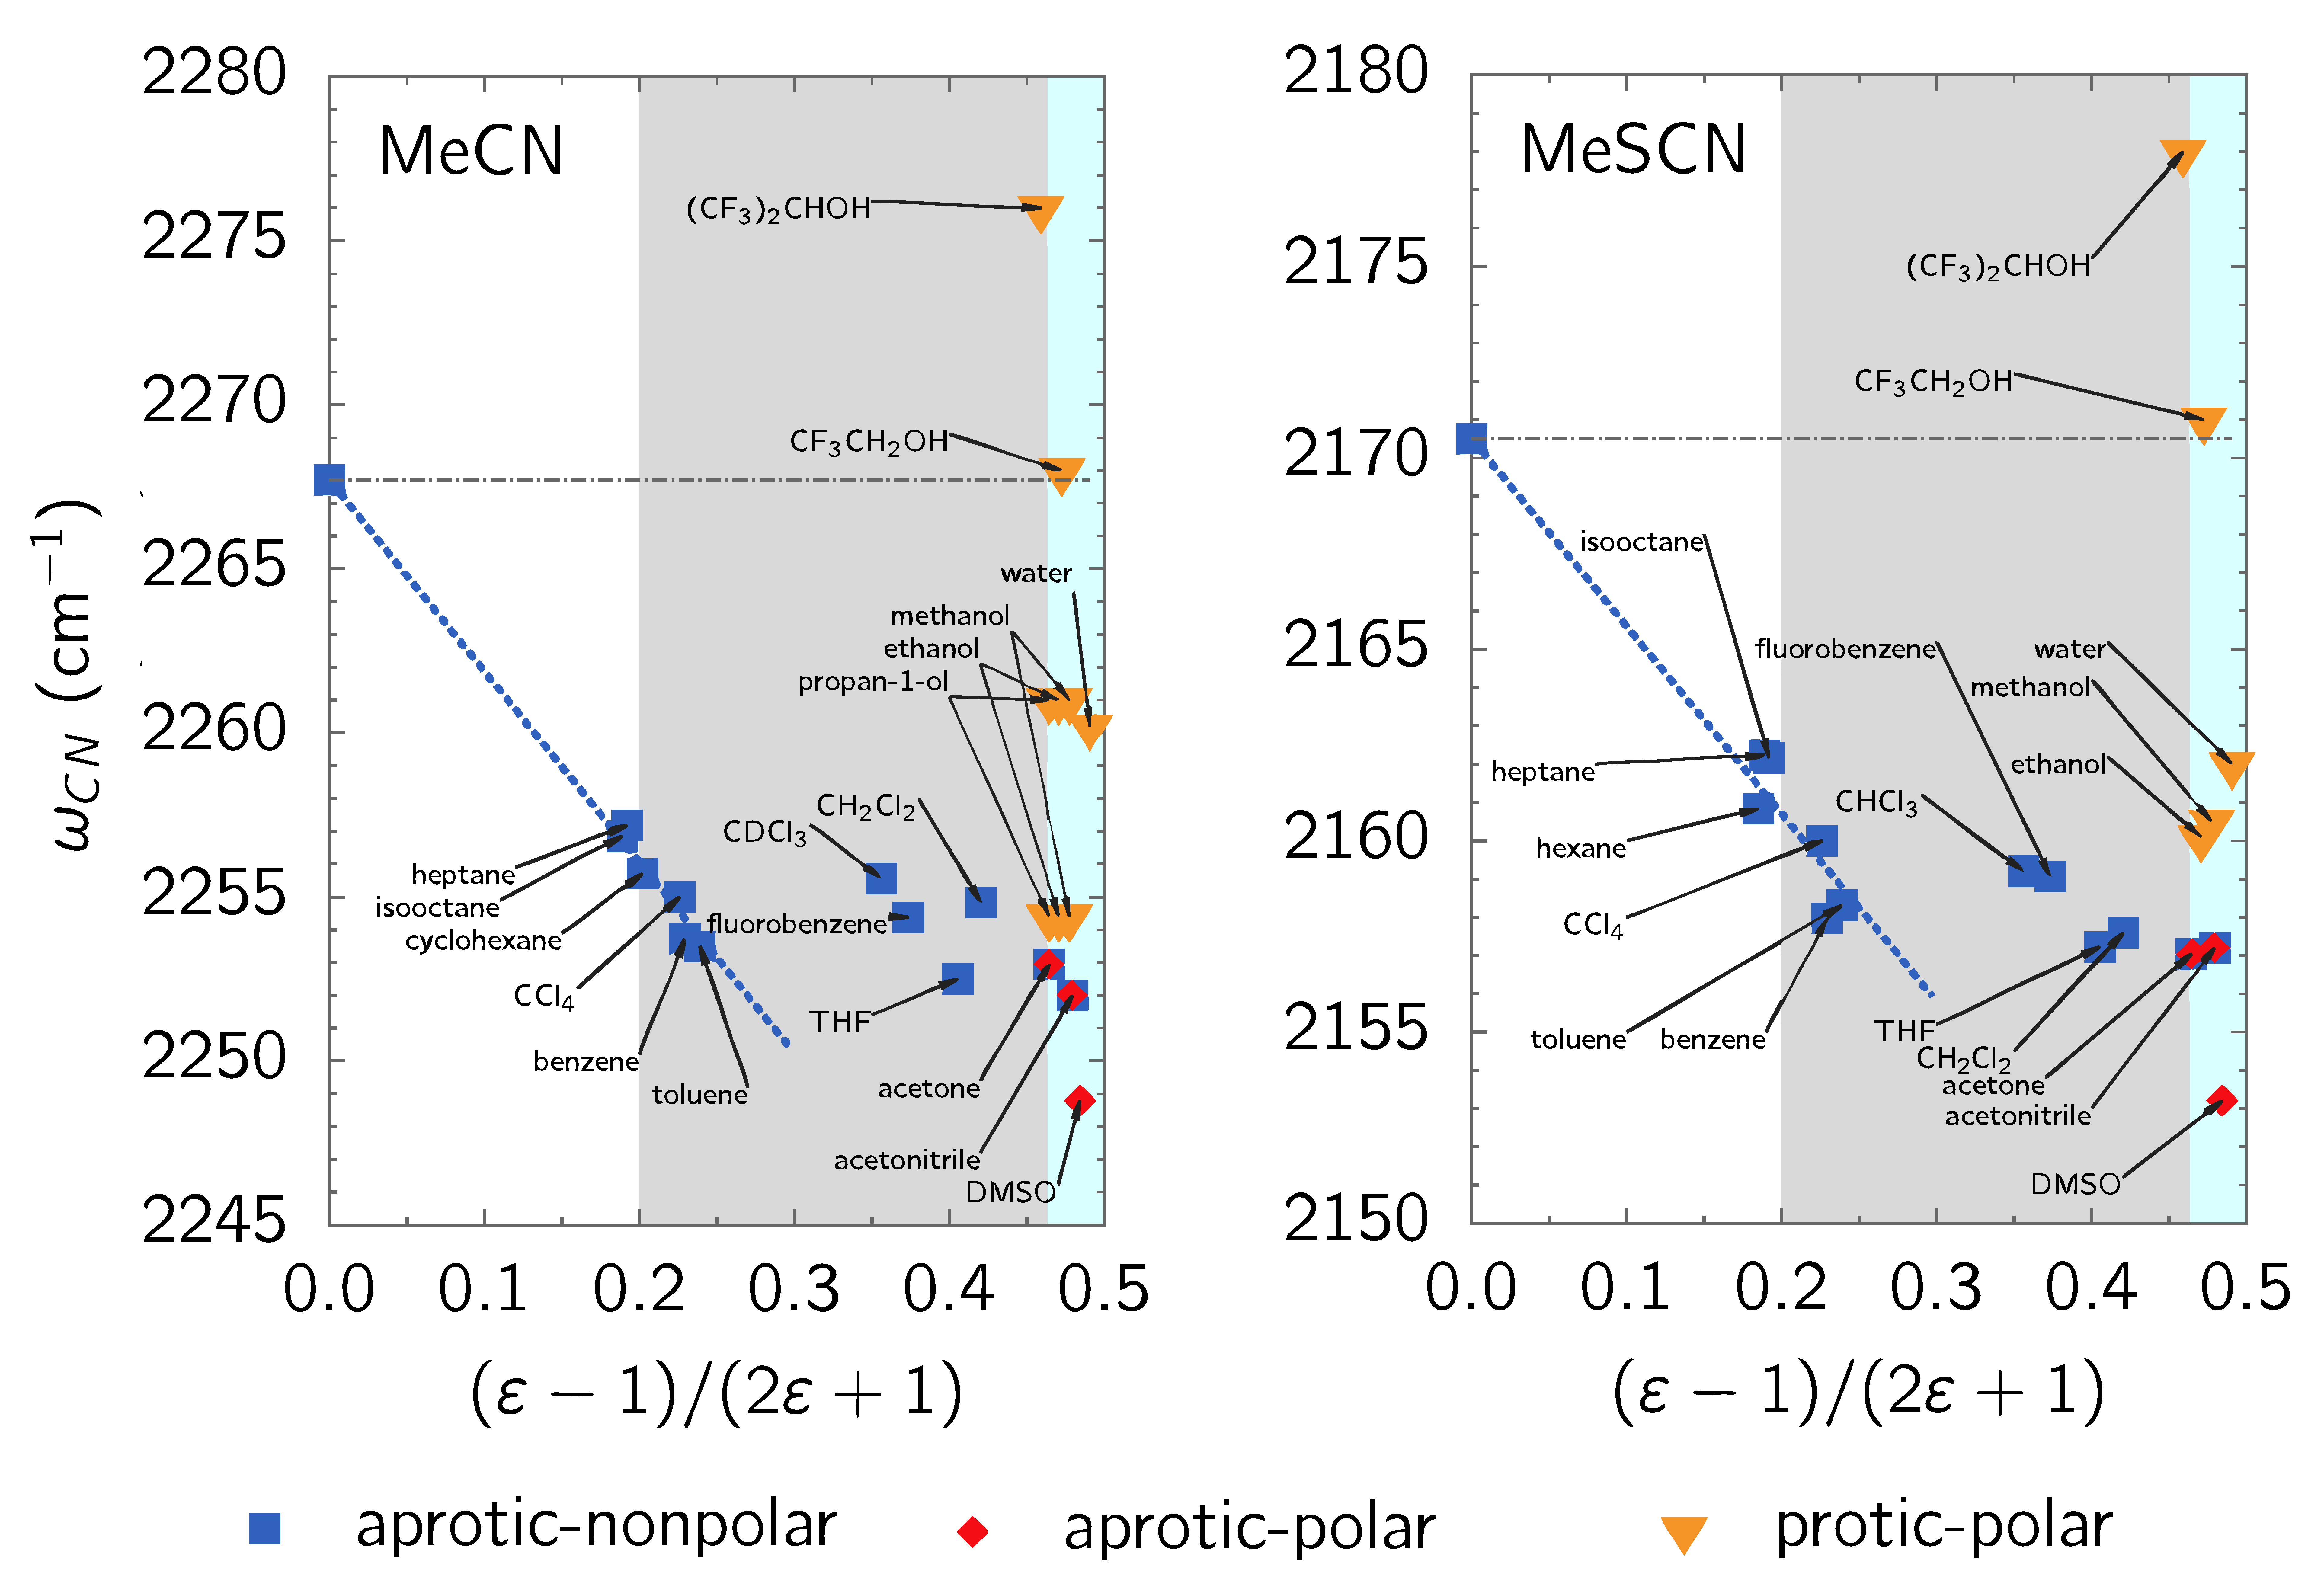
\includegraphics[width=0.9\linewidth]{Fig.1.eps}
}
\caption{Experimental frequencies of CN stretch mode of MeCN and MeSCN dissolved in
various solvents at room temperature. In this Figure, $\varepsilon$
stands for the solvent dielectric constant. Note that Onsager factor is zero in gas-phase. 
Frequencies that were not directly measured for this work were taken from the following 
References: MeCN in gas\hyp{}phase 
(Refs. \citep{Koga.Kondo.Saeki.Person.JPC.1984,Cerceau.Raulin.Courtin.Gautier.Icarus.1985,
Parker.Nielsen.Fletcher.JMS.1957}), 
MeCN in CCl$_4$, THF, MeOH, H$_2$O, CF$_3$CH$_2$OH and 
(CF$_3$)$_2$CHOH (Ref. \citep{Eaton.Pena-Nunez.Symons.JChemSocFaradTrans1.1988}), 
MeCN in CH$_3$(CH$_2$)$_2$OH (Ref. \citep{Oh.Choi.Lee.Han.Lee.Cho.JCP.2008}), 
MeSCN in gas-phase (Ref. \citep{Sullivan.Heusel.Durig.JMS.1984}), MeSCN in 
CCl$_4$, CHCl$_3$, CH$_2$Cl$_2$, MeCN, EtOH, MeOH, H$_2$O, CF$_3$CH$_2$OH and (CF$_3$)$_2$CHOH 
(Ref. \citep{Maienschein-Cline.Londergan.JPCA.2007}). In the 
cases of solvents with vanishingly small dipole moment (heptane, hexane, cyclohexane, 
isooctane, CCl$_4$), the linear relationship between CN frequency and Onsager factor indicates that 
the Kirkwood-Bauer-Magat law (blue line) works well. 
See Figure~\ref{f.MeCN.MeSCN.vs.solvents.spectra} for FTIR spectra.
\label{f.MeCN.MeSCN.vs.solvents}}
\end{figure}
%

As can be seen, for aprotic and non\hyp{}polar solvents, the linear dependence of
nitrile frequency shift on the Onsager factor is evident, suggesting the validity of the KBM theory.
It is a great success of the apparently simplistic continuum model of solvation. 
However, as the solvent polarity increases, the reaction field 
theory for vibrational solvatochromism fails. Furthermore, as the H-bond donating ability of 
solvent molecule increases, the nitrile stretch frequency becomes strongly blue-shifted, as 
compared to those in DMSO for instance. \citep{Wilderen.Luuk.Kern-Michler.Muller-Werkmeister.Bredenbeck.PCCP.2014}
This just indicates that the continuum representation of the surroundings is not acceptable in general
because of the neglect of the, so called, specific solvation effects. 
They include the direct solute\hyp{}solvent intermolecular
contacts like collisions, directional electrostatic interactions and weak bonding (for instance, hydrogen- (H-) bonding).
Nevertheless, it is clear that vibrational frequency may be fairly sensitive 
to the solvent used, even when the change of the polarity is small.

The solvation of many simple molecules was studied experimentally in detail from the perspective of the 
vibrational properties of some particular localised vibration. \citep{Rowlen.Harris.AnalChem.1991,Mayne.Hudson.JPC.1991,
Janroz.Stangret.Lindgren.JACS.1993,Akiyama.Ohtani.SpectchimActA.1994,
Reimers.Hall.JACS.1999,Wilderen.Luuk.Kern-Michler.Muller-Werkmeister.Bredenbeck.PCCP.2014,Jansen.JPCB.2014} 
Owing to the vibrational solvatochromism
like in Fig.~\ref{f.MeCN.MeSCN.vs.solvents}, 
appropriately chosen vibrational chromophores, which can be either a small molecule or a small functional
group, can be used as a local reporters of their vicinity. \citep{Kim.Cho.ChemRev.2013} 
We shall refer to such interesting chromophores as to the infrared (IR) probes. 

\section{Infrared Probes}

Throughout the years, there have been quite a few IR probes found or synthesised, and
they are nowadays widely used to study various molecular environments, starting from bulk solutions
to proteins, nucleic acids and other polymers. \citep{Kim.Cho.ChemRev.2013,
Ma.Pazos.Zhang.Culik.Gai.AnnuRevPhysChem.2015,Waegele.Culik.Gai.JCPL.2011}
Among the functional groups that have been demonstrated to be useful IR probes
are carbonyl (CO) \citep{Fried.Bagchi.Boxer.Science.2014,Thielges.Axup.Wong.Lee.Chung.Schultz.Fayer.JPCB.2011}, 
nitrile (CN) \citep{Zhang.Markiewicz.Doerksen.Smith.Gai.PCCP.2015,Johnson.Londergan.Charkoudian.JACS.2014,
Waegele.Culik.Gai.JCPL.2011,Stafford.Ensign.Webb.JPCB.2010,
Silverman.Pitzer.Ankomah.Boxer.Fenlon.JPCB.2007,Suydam.Snow.Pande.Boxer.Science.2006},
asymmetric azide (N$_3$) \citep{Thielges.Axup.Wong.Lee.Chung.Schultz.Fayer.JPCB.2011,
Ye.Zaitseva.Caltabiano.Schertler.Sakmar.Deupi.Vogel.Nature.2010,Waegele.Culik.Gai.JCPL.2011,
Taskent-Sezgin.Chung.Banerjee.Nagarajan.Dyer.Carrico.Raleigh.AngewChemInt.2010,Oh.Lee.Joo.Han.Cho.JPCB.2008} 
stretches, phosphate vibrations \citep{Levinson.Bolte.Miller.Corcelli.Boxer.JACS.2011}
and vibrations within nitro (NO$_2$) group \citep{Smith.Linderman.Luskin.Brewer.JPCB.2011}. 
Unique examples of using simultaneously two localised IR probes
were also reported. \citep{Thielges.Axup.Wong.Lee.Chung.Schultz.Fayer.JPCB.2011}
Those IR probes
generally fulfil the most important requirements for making it a useful tool: i) their transition
frequency is in the spectrally clean region, ii) their oscillatory strength is strong enough
to make them visible in the spectrum and analyse the signal, iii) the line shape 
of the resulting absorption peak is relatively easy to understand and has reasonably
narrow band width. 

Within the carbonyl IR probes, the first ever considered were the amide I modes
naturally occurring in proteins which are mostly the vibrations of the peptide group (CONH). Since
there is a lot of CONH groups in a protein, amide I modes can couple with each other
giving rise to the exciton bands in the IR spectra. This feature enabled to study 
the 3D structures of proteins with a combination of transition density
models \citep{Hayashi.Mukamel.JPCB.2007} because the coupling strongly depends 
on the relative orientation of transition dipoles. 
The problem with amide I mode (or amide I' when the proton becomes deuterated)
is that the bandwidth is still relatively broad. In addition, it is impossible to
obtain the local structural information due to the couplings.

Different strategy of using IR probes is related to isolated CO, CN or N$_3$ groups.
CO groups can be genetically encoded
such as CO bound to heme metal centre in myoglobin. 
CN and N$_3$ probes can be also site-selectively introduced into a macromolecular 
framework \citep{Jo.Culik.Korendovych.DeGrado.Gai.Biochem.2010,
Wang.Winblade.Johnson.Tirrell.Grabstein.ChemBioChem.2008,Fafarman.Webb.Chuang.Boxer.JACS.2006,
Kiick.Saxon.Tirrell.Bertozzi.PNAS.2002} 
which also provides
a local sond of the molecular environment. In particular, when such IR probe
is inserted into an active site of an enzyme, it becomes possible to study
how the enzyme acts within picosecond time scales. \citep{Fried.Bagchi.Boxer.Science.2014,Bagchi.Boxer.Fayer.JPCB.2012,
Ye.Zaitseva.Caltabiano.Schertler.Sakmar.Deupi.Vogel.Nature.2010} 
Another attractive way is to study protein structural fluctuation dynamics
or the protein-protein contacts when IR probe is localised at the protein 
surface \citep{Taskent-Sezgin.Chung.Banerjee.Nagarajan.Dyer.Carrico.Raleigh.AngewChemInt.2010,
Stafford.Ensign.Webb.JPCB.2010,Oh.Lee.Joo.Han.Cho.JPCB.2008}.  

\section{Understanding the Vibrational Solvatochromism}
%
However, the most fundamental issue that needs to be addressed 
before any IR probe is used, is what actually causes the vibrational solvatochromism.
Definitely, the electrostatic effects were considered to be the most important
(c.f. the KBM model) and much efforts were made to study the effects of the external
electric fields on the vibrational properties. \citep{Kim.Cho.ChemRev.2013} 
In particular, the effects of the
uniform external electric field was thoroughly examined. \citep{Hush.Reimers.JPC.1995,
Reimers.Zeng.Hush.JPC.1996,Andrews.Boxer.JPCA.2002,Cho.JCP.2009} 
In the vibrational Stark spectroscopy (VSE) \citep{Hush.Reimers.JPC.1995,Reimers.Zeng.Hush.JPC.1996}, 
which was pioneered experimentally by Boxer's laboratory \citep{Bublitz.Boxer.AnnuRevPhysChem.1997}, 
the change of the frequency, absorbance
and line shape is measured when the uniform external electric field is applied in certain fixed direction.
Under this circumstance, the frequency shift
was shown to be related to the electric field as follows \citep{Hush.Reimers.JPC.1995,Reimers.Zeng.Hush.JPC.1996}
%
\begin{equation} \label{e:vse-shift-full}
 \Delta \omega \approx - \Delta {\BM \mu} \cdot {\bf F} - \frac{1}{2} \Delta {\BM \alpha} : {\bf F} \otimes {\bf F}
\end{equation}
%
where $\Delta {\BM \mu}$ is, so called, the Stark tuning rate
and $\Delta {\BM \alpha}$ accounts for the quadratic effect with respect to 
the electric field, ${\bf F}$. 
Based on the VSE measurements, for the conventional
electric fields that exist inside biomolecules, the quadratic term
can be safely neglected. 
% CHECK THIS:
%For example, for the maximal electric field
%value reported so far (~160 MV/cm\citep{Fried.Bagchi.Boxer.Science.2014}) and the (assumed) upper bound for 
%$\Delta \alpha=1\times10^{-6}$ 
%cm$^{-1}\times \left({\rm cm}/{\rm MV}\right)^2$\citep{Andrews.Boxer.JPCA.2000,Andrews.Boxer.JPCA.2002}, 
%the frequency shifts is less than 0.03 cm$^{-1}$. For the sake 
%of comparison, the frequency shifts caused by linear term in Eq.~\eqref{e:vse-shift-full}
%can range from 3--100 cm$^{-1}$.
This fact gave rise to the dipole approximation (VSE-d)
widely used by VSE spectroscopists,
%
\begin{equation} \label{e:vse-shift-dipole}
 \Delta \omega \approx - \Delta {\BM \mu} \cdot {\bf F}
\end{equation}
%
Stark tuning rates have been reported for many IR probes. \citep{Suydam.Boxer.Biochem.2003,Levinson.Fried.Boxer.JPCB.2012}
They also were computed by using quantum chemistry calculations \citep{Dalosto.Vanderkooi.Sharp.JPCB.2004,
Andrews.Boxer.JPCA.2002,Andrews.Boxer.JPCA.2000}
and they are typically in a range of 0.4-1.0 cm$^{-1}$/(MV/cm). 
Since Eq.~\eqref{e:vse-shift-dipole} is proportional to solute's
dipole property, VSE-d have been correlated with Onsager's dipole
continuum model. For some subset of aprotic and non-polar
solvents descent linear correlation was found. \citep{Levinson.Fried.Boxer.JPCB.2012} 
Unfortunately,
when strongly protic solvents are used the significant deviations
from the linear correlations were observed. \citep{Fafarman.Sigala.Herschlag.Boxer.JACS.2010,Bagchi.Fried.Boxer.JACS.2012}

However, the serious drawback of VSE lies in the neglect of the field gradients that are 
likely to occur in the condensed phase. In fact, it was demonstrated theoretically
by Cho \citep{Cho.JCP.2009,Lee.Choi.Cho.JCP.2012} 
that when electric field varies in space, Eq.~\eqref{e:vse-shift-dipole}
has to be extended to account properly for field gradients,
%
\begin{equation} \label{e:vse-shift-multipoles}
 \Delta \omega 
\approx 
             - \Delta {\BM \mu}    \cdot                                {\bf F} 
- \frac{1}{3}  \Delta {\BM \Theta} :                     \nabla \otimes {\bf F}
- \frac{1}{15} \Delta {\BM \Omega} \vdots \nabla \otimes \nabla \otimes {\bf F}
+ \ldots
\end{equation}
%
where the appropriate \emph{solvatochromic multipoles} 
($\Delta {\BM \mu}$, $\Delta {\BM \Theta}$, $\Delta {\BM \Omega}$)
interact with the electric field (${\bf F}$), 
field gradient ($\nabla \otimes {\bf F}$), gradient of field gradient 
($\nabla \otimes \nabla \otimes {\bf F}$),
and so forth.
Another problem is related with the crude simplification of the 
molecular surroundings which is treated with continuum Onsager's model.
Despite all that, VSE is still being vividly
used by researchers to probe local electric fields in enzymes, DNA strands and 
lipid layers. 

There is yet another unclear issue which is associated with the electric field
used during the VSE experiment in order to determine Stark tuning rate.
It was shown that actually ${\bf F}$ is not perfectly constant but varies
near the molecule. The reason for this is the local field effect that arises
from the response of the molecule that is exposed to the perturbing electric field.
This phenomenon is difficult to assess quantitatively. Therefore, 
the empirical scaling factor, so called local field correction factor, $f$, 
was introduced to modify Eq.~\eqref{e:vse-shift-dipole} as follows
%
\begin{equation} \label{e:vse-shift-dipole-corr}
 \Delta \omega \approx - f \Delta {\BM \mu} \cdot {\bf F}
\end{equation}
%
According to continuum Lorentz model, $f$ is given by \citep{Wortmann.Bishop.JCP.1998}
%
\begin{equation}
f(\omega) = \frac{n^2(\omega)+2}{3}
\end{equation}
%
where $n(\omega)$ is the frequency\hyp{}dependent refractive index.
In the limiting case $\omega=0$ $f$ can be also expressed according to Onsager
model as \citep{Wortmann.Bishop.JCP.1998}
%
\begin{equation}
f(0) = \frac{\varepsilon (n^2(0)+2)}{n^2(0)+2\varepsilon}
\end{equation}
%
which extends Lorentz expression by including also orientational polarization effects
but refers to static limit.
It was deduced that $f$ can be in the range of 1.1-1.3 \citep{Wortmann.Bishop.JCP.1998,
Bublitz.Boxer.AnnuRevPhysChem.1997}, although
it is unclear whether this is always the case.

It is possible to combine the vibrational spectroscopy of IR probes (mostly VSE) with nuclear magnetic 
resonance (NMR) technique, which was demonstrated by Boxer's 
group. \citep{Fafarman.Sigala.Herschlag.Boxer.JACS.2010,Bagchi.Fried.Boxer.JACS.2012} 
It enables one
to separate out the contributions from the H\hyp{}bonding and other effects. However, 
it is very difficult to use this technique since it refers to empirical observables only,
and hence, one cannot get any detailed insight into the intricacies of the molecular granularity
and types of residues around an IR probe.

A few empirical models of the vibrational solvatochromism has been developed throughout the years.
They employ a variety of fitting procedures with a few adjustable parameters. For example, 
models based on certain molecular descriptors such as polarity, Lewis\slash{}Br{\o}nsted acidity\slash{}basicity, 
H-bonding donating\slash{}accepting ability were shown to be quite useful in relating the vibrational
frequency and infrared intensity with the type of solvent used. Among many methods of this kind,
perhaps the simplest one 
%The modern version of this extremely simplistic theoretical approach
is the Onsager model of the vibrational solvatochromism which
takes the form
%
\begin{equation} \label{e:vibr-onsager}
\Delta \omega(\varepsilon,n) \approx - \frac{2(\varepsilon-1)(n^2+2)}{3(2\varepsilon+n^2)} \frac{1}{V}
 \mu_0\Delta\mu
\end{equation}
%
where $V$ is the molecular volume, $n$ is the solute's refractive index
(crude approximation of its polarizability from classical point of view),
$\mu_0$ is the solute's dipole moment and $\Delta\mu$ is 
Stark tuning rate. \citep{Levinson.Fried.Boxer.JPCB.2012}
One should also mention models based on the
Kamlet\hyp{}Taft parameters \citep{Kamlet.Taft.JACS.1976,Taft.Kamlet.JACS.1976,Kamlet.Abboud.Taft.JACS.1977}, 
Fawcett's molecular descriptor method \citep{Reimers.Hall.JACS.1999,
Fawcett.Liu.Kessler.JPC.1993,Fawcett.Kloss.JCP.1996} or Ben-Amotz' theory. \citep{Ben-Amotz.Lee.Cho.List.JCP.1992} 
The latter is actually derived from first principles, but it was mostly used by fitting
the resulting parameters to the experiment rather that explicitly obtaining them from calculations.
%We will talk about the Ben-Amotz \emph{et al.}'s model in more detail later (Section~XXX) because it is the first
%truly first\hyp{}principles model that decomposes the frequency shifts into not only electrostatic, 
%but also non\hyp{}electrostatic repulsive contributions.
The Ben-Amotz \emph{et al.}'s model is the first
truly first\hyp{}principles model that decomposes the frequency shifts into not only electrostatic, 
but also non\hyp{}electrostatic repulsive contributions.

In KT parameter method, frequency shifts can be related to the following
relation \citep{Zhang.Markiewicz.Doerksen.Smith.Gai.PCCP.2015}:
%
\begin{equation} \label{e:kamlet-taft}
\Delta \omega = A\alpha + B\beta + C\pi^{*}
\end{equation}
%
In this approach, one has to
find the coefficients $A$, $B$ and $C$ that are fitted against
the solute's KT parameters $\alpha$ \citep{Taft.Kamlet.JACS.1976}, 
$\beta$ \citep{Kamlet.Taft.JACS.1976} and $\pi^{*}$ \citep{Kamlet.Abboud.Taft.JACS.1977} 
describing the hydrogen bond accepting,
hydrogen bond donating, and dielectric interactions abilities, respectively.
KT parameters were originally determined from VIS spectra and related different
spectroscopic observables into one multivariate linear relationship as in Eq.~\eqref{e:kamlet-taft}.

Slightly more complicated parametrisation was developed 
by Fawcett~\emph{et al.} \citep{Reimers.Hall.JACS.1999,Fawcett.Liu.Kessler.JPC.1993,Fawcett.Kloss.JCP.1996},
in which the solute's frequency shift\footnote{originally acetonitrile $\nu_2$ frequency
which is CN stretch mode} can be expressed by the mix of solute- and
solvent-related empirical descriptors
%
\begin{multline} \label{e:fawcett}
\Delta \omega = \Delta \omega_{gp} + 
\left( a_{Sol} - a_{St} \right) A_A +
\left( d_{Sol} - d_{St} \right) A_D \\ + 
\left( \frac{\varepsilon_{Sol}-1}{\varepsilon_{Sol}+2} - \frac{\varepsilon_{St}-1}{\varepsilon_{St}+2} \right) A_\varepsilon +
\frac{3}{4\pi}
\left( \frac{n^2_{Sol}-1}{n^2_{Sol}+2} - \frac{n^2_{St}-1}{n^2_{St}+2} \right) A_\alpha
\end{multline}
%
In the above formula, $\Delta \omega_{gp}$ denotes the frequency shift in pure liquid of solute
relative to the gas phase,
$a$ and $d$ are the Gutmann solvent acceptor and donor numbers \citep{Gutmann.Resch.Linert.CoordChemRev.1982}, 
respectively,
and the associated four constants $A_A$, $A_D$, $A_\varepsilon$ and $A_\alpha$ 
are to be fit to the experimentally determined frequency shifts in different solvents.
The lower indices $St$ and $Sol$ indicate solute and solvent parameters, respectively. 
Note that all fitting parameters in Eqs.~\eqref{e:kamlet-taft} and ~\eqref{e:fawcett} 
describe the solute\hyp{}solvent interactions empirically.

In his seminal works, Ben\hyp{}Amotz~\emph{et al.} \citep{Ben-Amotz.Lee.Cho.List.JCP.1992} 
used the first\hyp{}principles theory of Buckingham \citep{Buckingham.ProcRSocLondonA.1958,
Buckingham.ProcRSocLondonA.1960,Buckingham.TransFaradaySoc.1960}
to derive the contributions to the vibrational frequency shift due to
repulsive, attractive and centrifugal distortion forces. Mainly,
%
\begin{equation} \label{e:ben-amotz}
 \Delta \omega = \Delta \omega_R + \Delta \omega_A + \Delta \omega_C
\end{equation}
%
It was concluded that the repulsive part $\Delta \omega_R$ is more or less constant
and constitutes about 4 cm$^{-1}$ to the blue shift. Attractive part, $\Delta \omega_A$,
was attributed to the dispersion and dipole\hyp{}dipole interactions
and was shown to be proportional to the solvent density as
%
\begin{equation} \label{e:ben-amotz-ro}
 \Delta \omega = 2\pi\left( A_\alpha \alpha_S + A_\mu \mu_S^2 \right) \rho_S
\end{equation}
%
in which constants $A_\alpha$ and $A_\mu$ could be determined empirically. 
In the above equation, $\rho_S$ is the solvent density whereas $\mu_S$ and $\alpha_S$ are the
dipole moment magnitude and isotropic polarizability of the solvent molecules.

The centrifugal distortion effect on acetonitrile CN stretch frequency 
caused by inhibited rotation of solute molecules
in solution was estimated to be roughly --0.5 cm$^{-1}$ in the liquid phase.  
The empirical relationship in Eq.~\eqref{e:ben-amotz-ro} was proven to be not sufficient to obtain 
satisfactory correlations with experiment and more refined
models (such as Fawcett \emph{et al.}'s model) were necessary. \citep{Reimers.Hall.JACS.1999} 
Nevertheless, 
to the best of my knowledge, both the theory of Ben-Amotz~\emph{et al.} \citep{Ben-Amotz.Lee.Cho.List.JCP.1992} 
and the theory
developed later in this Thesis are the only first-principles theories on the
vibrational solvatochromism that explicitly take into account the electrostatic 
attractive and non\hyp{}Coulombic repulsive interactions.

Another important class of empirical or semi\hyp{}empirical methods which is broadly referred 
to as the electrostatic fitting methods (ESF), uses the correlation of benchmark 
\emph{ab initio} or density functional theory (DFT)-calculated vibrational properties
with electrostatic potential, electric field or its gradients, that are estimated at various
points in space around an IR probe. \citep{Kwac.Cho.II.JCP.2003,Ham.Kim.Lee.Cho.JCP.2003,Bour.Keiderling.JCP.2003,
Schmidt.Corcelli.Skinner.JCP.2004,Corcelli.Lawrence.Skinner.JCP.2004,Hahn.Lee.Cho.JCP.2004,Kwac.Lee.Cho.JCP.2004,
Choi.Hahn.Cho.IJQC.2005,Kwac.Cho.JRS.2005,Watson.Hirst.MP.2005,
DeCamp.DeFlores.McCracken.Tokmakoff.Kwac.Cho.JPCB.2005,Hayashi.Jansen.Zhuang.Mukamel.JPCA.2005,
Hayashi.Zhuang.Mukamel.JPCA.2005,Bour.Michalik.Kapitan.JCP.2005,
Jansen.Dijkstra.Watson.Hirst.Knoester.JCP.2006,
Jansen.Knoester.JCP.2006,
Choi.Oh.Lee.Lee.Cho.JCP.2008,Oh.Choi.Lee.Han.Lee.Cho.JCP.2008,
Choi.Oh.Cho.JCP.2008,
Lin.Shorb.Mukherjee.Zanni.Skinner.JPCB.2009,Lee.Choi.Cho.PCCP.2010,Choi.Cho.JCP.2011,
Roy.Lessing.Meisl.Ganim.Tokmakoff.Knoester.Jansen.JCP.2011,Choi.Raleigh.Cho.JCPL.2011,
Lee.Choi.Cho.JCP.2012,Torii.JCPL.2015,Torii.Noge.PCCP.2016}
%
The method can be generally described by the following empirical relationship
%
\begin{equation} \label{e:esf}
 P(\phi \text{ or } {\bf F}) = \sum_X \left\{ l_X \phi_X + {\bf d}_X \cdot {\bf F}_X + {\bf D}_X : \nabla \otimes {\bf F}_X \right\}
\end{equation}
%
where $P$ is the property in question (frequency, transition dipole and so on), 
$\phi_X$ and ${\bf F}_X$ are the electrostatic potential and electric field, respectively, that are
evaluated at some point $X$.
These points are called `interaction centres' and their
choice is mostly a matter of pure convenience in order to obtain a reliable and efficient
fitting model ($l_x$, ${\bf d}_x$, ${\bf D}_x$ parameter set). Mostly, only one type of parameters
(e.g. scalar by Cho's and Bou\v{r}'s groups \citep{Kwac.Cho.II.JCP.2003,Ham.Kim.Lee.Cho.JCP.2003,
Bour.Keiderling.JCP.2003,Hahn.Lee.Cho.JCP.2004,Kwac.Lee.Cho.JCP.2004,
Choi.Hahn.Cho.IJQC.2005,Kwac.Cho.JRS.2005,
Choi.Oh.Lee.Lee.Cho.JCP.2008,Oh.Choi.Lee.Han.Lee.Cho.JCP.2008,
Choi.Oh.Cho.JCP.2008,Lee.Choi.Cho.PCCP.2010,Choi.Cho.JCP.2011,
Choi.Raleigh.Cho.JCPL.2011,Lee.Choi.Cho.JCP.2012}
or vector by Skinner's group \citep{Schmidt.Corcelli.Skinner.JCP.2004,
Corcelli.Lawrence.Skinner.JCP.2004}) is employed, but there are also maps utilising multiple types of parameters
as well (scalar + vector by Torii's group \citep{Torii.JCPL.2015,Torii.Noge.PCCP.2016} 
or vector + vector gradient by Jansen and Knoester \citep{Jansen.Knoester.JCP.2006}
and Mukamel's group \citep{Hayashi.Jansen.Zhuang.Mukamel.JPCA.2005,Hayashi.Zhuang.Mukamel.JPCA.2005}).
 
In practice, the spectator molecule in question is often solvated by a relatively small number of polar 
solvent molecules that create varying electrostatic potential. \citep{Bour.Keiderling.JCP.2003,
Lin.Shorb.Mukherjee.Zanni.Skinner.JPCB.2009,
Lee.Choi.Cho.JCP.2012} 
The perturbing fields can also be applied directly
in many directions. \citep{Jansen.Dijkstra.Watson.Hirst.Knoester.JCP.2006,
Jansen.Knoester.JCP.2006,Roy.Lessing.Meisl.Ganim.Tokmakoff.Knoester.Jansen.JCP.2011,
Hayashi.Jansen.Zhuang.Mukamel.JPCA.2005,
Hayashi.Zhuang.Mukamel.JPCA.2005,Bour.Michalik.Kapitan.JCP.2005} 
It is also possible to account for molecular anharmonicity
when the model gas\hyp{}phase Hamiltonian with polynomial expansion of anharmonic potential
is used and perturbed by external electric fields. \citep{Jansen.Knoester.JCP.2006}
Subsequent multivariate
least-square analyses of these model systems are then performed to obtain the vibrational 
solvatochromic parameters (or maps) for a given IR probe molecule, from which the benchmark
results could be reproduced. 

Despite it was reported that ESF approach can be very accurate in reproducing the frequency shifts and even
transition dipoles, we pointed out that the fitting procedures
can be biased towards a chosen subset of systems or molecular environments. This obviously can limit
the transferability and universality of the method, unless the reference data is `complete enough'
to cover all relevant solute\hyp{}solvent interaction scenarios. Note that the ESF approach intrinsically
assumes that the only driving force of the vibrational solvatochromism is \emph{electrochromism}
and all other aspects of intermolecular interactions like van der Waals forces and dispersion are
ignored in the theoretical formulation. On the other hand, since ESF is based on fitting, it is 
possible that also non\hyp{}electrostatic effects are captured by this method when calculating the benchmark 
vibrational frequencies of solute\hyp{}solvent clusters. This may cause serious problems with the interpretations
of the frequency shifts based on ESF. If non\hyp{}electrostatic contributions affect the fitting
parameters, the conclusions about the structural features of the systems could be incorrect 
because ESF assumes electrostatic functional form (strongly solute\hyp{}solvent orientation\hyp{}dependent).\footnote{
The same problem refers to VSE-d approximation from Eq.~\eqref{e:vse-shift-dipole-corr}.
If there are other terms contributing to frequency shift like quadrupolar terms 
in Eq.~\eqref{e:vse-shift-multipoles} the conclusions based
on the analysis of VSE data are incorrect.}

There are a few reports showing that the ESF parameters can achieve the level of solvent
and even solute transferability. \citep{Kwac.Lee.Cho.JCP.2004,
DeCamp.DeFlores.McCracken.Tokmakoff.Kwac.Cho.JPCB.2005,Jansen.Knoester.JCP.2006,
Choi.Raleigh.Cho.JCPL.2011} However, it is not at all clear to what extent the universality is
preserved, especially when the change of environment is drastic. For example, let us consider putting a probe in
a completely non\hyp{}polar solvent such as CCl$_4$ which has no net molecular dipole moment. 
Then, let us apply an ESF map that was derived in aqueous solutions (which is mostly the case in this kind
of parameterizations). Since CCl$_4$ molecules are rather unlikely to exert strong electrostatic fields 
around IR probe we might expect very small frequency shifts. But the examples of MeCN and MeSCN probes
dissolved in this solvent (Figure~\ref{f.MeCN.MeSCN.vs.solvents}) 
show the very pronounced frequency red shifts that are roughly --10 cm$^{-1}$
relative to the gas phase, which is comparable to frequency shifts in water! 
We will show later that it is basically impossible by using a purely electrostatic approach
to capture these mysterious effects that cause so strong red shifts in the case of CN stretch in non\hyp{}polar
solvent. It is also not so clear whether electrostatic map from Eq.~\eqref{e:esf} is able to 
encapsulate those effects into the fitting parameters.

Different from ESF methods approach is the re\hyp{}parameterization of the original semi\hyp{}empirical 
quantum Hamiltonian and its bath\hyp{}coupling parameters specifically to the problem of interest,
that was proposed by Skinner's group \citep{Li.Schmidt.Corcelli.Lawrence.Skinner.JCP.2006}
and then developed by Corcelli's group \citep{
Lindquist.Corcelli.JPCB.2008,Lindquist.Haws.Corcelli.JPCB.2008,
Lindquist.Furse.Corcelli.PCCP.2009}. Their method which is based on PM3 Hamiltonian, \citep{Stewart.JCC.1988}
was shown to be useful and quite transferable between various solutes and solvents. 
It cab also be interfaced with the molecular mechanics approach (OQM/MM) \citep{Lindquist.Haws.Corcelli.JPCB.2008}
to probe the dynamics (at the PM3/MM level) and the vibrational solvatochromism 
at the same level of theory.
However, it requires complicated
parameterizations procedures.

It is also possible to use experimentally measured protein spectra directly 
as reference data. \citep{Karjalainen.Ersmark.Barth.JPCB.2012}
Such an approach is specifically designed for dealing with very large systems like proteins and
can be very accurate. Unfortunately, it provides no physical interpretation of the observed
spectral signals and has only predictive power.



\section{Signs of Non-Electrostatic Vibrational Solvatochromism\label{s:signs-non-elect-solv}}
As opposed to the bunch of studies concentrating on the electrostatic
approximation of the vibrational solvatochromism, there exist a few 
semi\hyp{}empirical works of the other effects that trigger frequency shift
changes upon solvation. 

Perhaps one of the first was the study of Ben-Amotz~\emph{et al.} in 1992. \citep{Ben-Amotz.Lee.Cho.List.JCP.1992}
They wanted to understand the relationship between the vibrational frequency
and the pressure. The first\hyp{}principles model built on the Buckingham's theoretical
foundations \citep{Buckingham.ProcRSocLondonA.1958,Buckingham.TransFaradaySoc.1960,
Buckingham.ProcRSocLondonA.1960} was used to obtain the empirical set of parameters fit to
experimental data of chosen vibrational frequencies in various solvents
and pressures. One of the most important findings of their study was
that the dispersion plays an important role in the vibrational barochromism
of acetonitrile CN stretch mode at low densities and repulsive interactions cause strong blue shifts
at higher densities.

In 1998, Reimers and Hall \citep{Reimers.Hall.JACS.1999} investigated in great detail the solvation of acetonitrile 
based on the Ben-Amotz~\emph{et al.}'s and Fawcett~\emph{et al.}'s models in solvents under standard atmospheric pressures. 
%It is surprising to me what they found.
From among 33 various solvents ranging from non\hyp{}polar and non\hyp{}protic CCl$_4$, 
through strongly protic
DMSO to quite acidic trifluoroacetic acid (TFA), they noticed that the electrostatic
non\hyp{}specific interactions cause much lesser redshifts as compared to the dispersion
interactions. Note that the latter cannot be correlated with electrostatic potential
or electric field at all. What is also interesting in their work is that they 
reported specific (short\hyp{}range) frequency \emph{blue shifts} which were strongly enforced
in solvents forming H-bonding interactions. In fact, the stronger H-bonds formed between MeCN
and solvent molecules, the larger this blue shift was obtained. For instance,
the non\hyp{}specific electrostatic, dispersion, and specific (electrostatic
and non\hyp{}electrostatic) vibrational frequency shifts of acetonitrile CN mode
in water were found to be --6.4, --9.7 and +6.7 cm$^{-1}$, whereas in CCl$_4$ they were
--1.9, --13.0 and 0.0 cm$^{-1}$, respectively.

Since, at that time it was impossible to discriminate between various short\hyp{}range
interactions, the physical nature of the mysterious blue shifts remained unknown.
However, there appeared other theoretical analyses of the CN frequency shifts of MeCN in water
or CN$^-$ anion in water. Rey and Hynes \citep{Rey.Hynes.JCP.1998} decomposed the forces obtained from classical molecular dynamics
(CMD) simulations and found that the van der Waals potential exerts strong blue shifts of CN mode in CN$^-$.
Similar conclusion was drawn by Morales and Thompson who investigated MeCN/water system by 
using CMD. \citep{Morales.Thompson.JPCB.2011}

The signs of non\hyp{}negligible exchange\hyp{}repulsion\hyp{}induced vibrational 
frequency shifts \newline were also  
found. \citep{Li.Liu.Schlegel.JACS.2002,Delanoye.Herrebout.vanderVeken.JACS.2002,Zierkiewicz.Jurecka.Hobza.ChemPhysChem.2005,
Rodziewicz.Rutkowski.Melikova.Koll.ChemPhysChem.2005,
Zhou.Qiu.JPCA.2009,Mo.Wang.Guan.Braida.Hiberty.Wu.ChemEurJ.2014}
It was shown by correlating the interaction
energy components [for example, from symmetry\hyp{}adapted 
perturbation theory \citep{Jeziorski.Moszynski.Szalewicz.ChemRev.1994} (SAPT)] with frequency shifts, that repulsive potentials
lead to blue shifts. For example, Zierkiewicz \emph{et al.} studied the series of 
blue\hyp{} and red\hyp{}shifting complexes. \citep{Zierkiewicz.Jurecka.Hobza.ChemPhysChem.2005} 
attributed the
blue shifting patterns to a ``repulsion wall'' caused by Pauli exclusion principle. 
Also, they noticed that
the dispersion effects can affect the vibrational frequency in various ways
and discriminated between two distinct mechanisms.

In 2005, Rodziewicz~\emph{et al.} has combined Buckingham's theory for a diatomic case approximation with SAPT 
and studied vibrations involving C--H or C--X
stretches, where X denotes halogen atom. \citep{Rodziewicz.Rutkowski.Melikova.Koll.ChemPhysChem.2005} 
They found that the exchange\hyp{}repulsion effects
cause blue shifts and the nature of these frequency shifts is quite complex. Also, dispersion
interaction\hyp{}induced red shifts were non\hyp{}negligible. 

In 2009, Choi~\emph{et al.} were studying the effects of charge transfer on the vibrational
frequency of the model ionic IR probes such as CN$^-$ or N$_3^-$ anions dissolved in water. \citep{Lee.Choi.Cho.PCCP.2010}
Although they found a considerable charge
transfer between solute\hyp{}water molecules, the total charge transferred appeared to be in no
correlation with the vibrational frequency shifts. This was interpreted that the charge transfer 
phenomenon can be neglected when considering the vibrational interaction\hyp{}induced frequency shifts
for the studied systems. However, charge transfer was found to be almost as important as electrostatic
interactions in the 
recent work of Brinzer \emph{et al.}, \citep{Brinzer.Berquist.Zhe.Dutta.Johnson.Krisher.Lambrecht.Garrett-Roe.JCP.2015} 
in which they studied CO$_2$ asymmetric
stretching ($\nu_3$) mode as an IR probe for sensing the local molecular environments in ionic
liquids. Moreover, it was demonstrated recently that the solvation\hyp{}induced vibrational
frequency shifts of pyrimidine's modes are very well correlated with charge transfer between
pyrimidine and eight various polar solvents including water, methanol
and hexylamine. \citep{Wright.Howard.Howard.Tschumper.Hammer.JPCA.2013}

\section{Summary}

From the brief literature review on the vibrational solvatochromism
that was presented above it is clear that the electrostatic effects
are not the only phenomena governing the interaction\hyp{}induced 
vibrational frequency shifts. There is in fact little work done
to understand the origins of the non\hyp{}Coulmbic effects and their
role in the spectral line shapes and positions and the comprehensive,
all\hyp{}encompassing vibrational solvatochromism theory is lacking. Apparently,
non\hyp{}Coulombic effects were mostly ignored when analysing and interpreting
the vibrational spectra.

In the forthcoming Chapters, we will present the general theory of the vibrational
solvatochromism that is not limited to the electrostatic approximation. 
In particular, the detailed fully first\hyp{}principles expressions
will be derived and shown 
that they can be used to calculate various contributions to the vibrational solvatochromic frequency
shifts directly by means of quantum chemistry calculations. We shall also test those equations 
and when combined with CMD we shall show that such a theory can quantitatively predict the
vibrational solvatochromism of many IR probes. We want to shed new light
on the importance of non\hyp{}Coulombic effects
in the vibrational solvatochromism.

\printbibliography[heading=subbibintoc,title={References}]
\end{refsection}

% ==== CHAPTER 3

\begin{refsection}
\chapter{Vibrational Solvatochromism Theory\label{c:background}}

As pointed out in previous Chapter, understanding the vibrational
solvatochromism requires a rigorous quantum mechanical treatment.
In this Chapter, we derive the fundamental theories of the vibrational
solvatochromism by analysing the Hamiltonian of an IR spectator molecule.
The frequency shift and transition dipole are then expressed as functions
of the solute\hyp{}solvent interaction potentials.

\section{Overview\label{s:theory}}

The rigorous first\hyp{}principles theory behind the vibrational solvatochromism was published
for the first time by Buckingham. \citep{Buckingham.ProcRSocLondonA.1958,
Buckingham.TransFaradaySoc.1960,Buckingham.ProcRSocLondonA.1960} 
In his seminal works, Buckingham found the fundamental 
relation between the solute\hyp{}solvent interaction energy change along normal 
coordinates, solute's anharmonicity and the vibrational frequency shifts.
His formula, although derived for the general $N$-atomic case, was tested
only for the diatomic approximation with only one normal mode. 
His theory was found to predict not only
the interaction\hyp{}induced frequency shift, but also structural deformation in simple
diatomic cases \citep{McDowell.Buckingham.MolPhys.2005,McDowell.Buckingham.JACS.2005,
McDowell.Buckingham.SpectrChimActaA.2005,Buckingham.CPL.2008} 
and also tri- and polyatomic molecules under 
vibrationally diatomic approximation. \citep{McDowell.Buckingham.SpectrChimActaA.2005,
Buckingham.CPL.2008,Herrebout.Delanoye.vanderVeken.JPCA.2004}

At the turn of \nth{20} century, Hush and Reimers \citep{Hush.Reimers.JPC.1995,Reimers.Zeng.Hush.JPC.1996} 
and Andrews and Boxer \citep{Andrews.Boxer.JPCA.2002,Andrews.Boxer.JPCA.2000} 
were considering the vibrational electrochromism
to quantitatively relate vibrational properties with the external electric fields.
In their theoretical foundations of the vibrational Stark spectroscopy,
they explained in detail the response of the molecular vibrational mode's frequency
and intensity
on the external electric field. 

Buckingham's the theory of the vibrational solvatochromism was rediscovered later 
by Cho. \citep{Cho.JCP.2003,Cho.JCP.2009} 
%though using different theoretical
%approach, he found essentially the same formulas for the frequency shifts as Buckingham, Hush
%and Reimers. 
However, Cho's 
approach focused on more practical application of the vibrational solvatochromism 
theory and enabled fragment\hyp{}based approach to this problem. In his coarse\hyp{}grained
model of vibrational solvatochromism, he showed that,
under electrostatic approximation based on the distributed multipole expansion, 
the vibrational frequency shift can be written in an analogous manner as the conventional
Coulomb interaction energy, i.e., a series of multipoles interacting with
electrostatic potential, electric field and its gradients. 
He constructed the first\hyp{}principle set of 
the \emph{solvatochromic multipole moments} that can be systematically used
to predict the electrostatic frequency shifts. Thus, this work opened a new route for developing
all\hyp{}encompassing theory based on single molecules in gas phase.

The theoretical dissertations of Buckingham and Cho were my stimuli and inspired
me to extend the coarse\hyp{}grained electrostatic vibrational solvatochromism 
model of Cho by the analysis of the other fundamental intermolecular interactions.
%exchange-repulsion, induction (polarization), dispersion and charge transfer (CT).
Therefore in the forthcoming sections, we will go through both Buckingham's and Cho's
models in detail
to derive the \emph{ab initio} expressions for the interaction\hyp{}induced 
vibrational frequency shifts that are not limited by electrostatic approximation.
Those theories will be a basis of later approach which is not limited to
Coulombic interactions, but includes other important intermolecular forces altogether
in a systematic way. Since the theory involves quite complicated
tensor notation, we encourage to read first the Appendix~\ref{a:tensor-notation}
for clarification of notational convention regarding tensor operations.
The Reader who is not familiar with the quantum theory of vibrations is strongly encouraged
to read the Appendix~\ref{a:vibrational-analysis} 
(especially Section~\ref{a:harmonic-oscillator})
in which the brief introduction to this fundamental aspect is presented.

\section{Buckingham's Model  \label{s:buckingham-theory}}

The starting point in Buckingham's consideration was to analyse 
the harmonic oscillator Hamiltonian which is perturbed by anharmonicity
and the interaction potential between solute and solvent molecules. Mainly,
%
\begin{equation}
\mathscr{H} = \mathscr{H}_{\rm Harm} + \mathscr{H}_{\rm Anh} + U({\bf Q}_A,{\bf Q}_B)
\end{equation}
%
where
%
\begin{equation}\label{e:h_harm}
\mathscr{H}_{\rm Harm} = 
\sum_i \frac{\mathscr{P}_i^2}{2M_i} + \frac{1}{2} M_i \omega_i^2 Q_i^2
\end{equation}
%
and
%
\begin{equation}\label{e:h_anh}
\mathscr{H}_{\rm Anh} = 
\sum_{ijk} \frac{1}{3!} g_{ijk} Q_iQ_jQ_k + \ldots 
\end{equation}
%
$Q_i$ denotes the $i$th normal coordinate of the solute in gas phase whereas
${\bf Q}_A$ and ${\bf Q}_B$ represent the structures of solute and solvent, 
respectively.

The solutions to the Schr{\"o}dinger equations for the solvated and 
unsolvated states can be written as
%
\begin{eqnarray}
\left[ \mathscr{H}_{\rm Harm} + \mathscr{H}_{\rm Anh} + U \right] 
\vert \Psi \rangle &=& W \vert \Psi \rangle \\
\left[ \mathscr{H}_{\rm Harm} + \mathscr{H}_{\rm Anh} \right] 
\vert \Gamma \rangle &=& G \vert \Gamma \rangle 
\end{eqnarray}
%
with $\vert\Psi\rangle$ and $\vert\Gamma\rangle$ representing the solute's wavefunctions
in its solvated and gas\hyp{}phase states, respectively.

Since the exact solutions of the Schr{\"o}dinger equations are known 
for $\mathscr{H}_{\rm Harm}$, Buckingham used the perturbation theory
to derive the effects on the vibrational energies upon binding with solvent
molecule. % (here abbreviated as $B$).
In other words, he assumed that
%
\begin{equation} \label{e:RSPT-Hamiltonian}
\mathscr{H} = \mathscr{H}^{(0)} + \mathscr{H}'
\end{equation}
%
where the zeroth\hyp{}order Hamiltonian $\mathscr{H}^{(0)}=\mathscr{H}_{\rm Harm}$
and the perturbation operator 
%
\begin{subequations} \label{e:RSPT-Hamiltonian:perturbation}
\begin{align}
\mathscr{H}'&=\mathscr{H}_{\rm Anh} + U({\bf Q}_A,{\bf Q}_B)  & \text{(solution)}\\
\mathscr{H}'&=\mathscr{H}_{\rm Anh}                           & \text{(gas phase)}
\end{align}
\end{subequations}
%
The zeroth\hyp{}order energies are given by
%
\begin{equation}
E_{n,j}^{(0)} = \hbar \omega_j \left( n_j+\frac{1}{2} \right)
\end{equation}
%
Since the series expansions along $Q_i$ are used in Eqs.~\eqref{e:h_harm}
and~\eqref{e:h_anh}, the solute\hyp{}solvent interaction potential
should also be expanded:
%
\begin{equation}\label{e:u_taylor}
U({\bf Q}_A,{\bf Q}_B) = 
U_0 + \sum_i \frac{\partial U}{\partial Q_i} \Bigg|_{{\bf Q}_{0_A}} Q_i
+ \frac{1}{2} \sum_{ij} \frac{\partial^2 U}{\partial Q_i \partial Q_j} \Bigg|_{{\bf Q}_{0_A}} Q_i Q_j
+ \ldots
\end{equation}
%
where $U_0$ is a constant offset.\footnote{
%
In this Work, we sometimes use a shorthand notation for the derivatives
of $U$ such that the $n$th derivative $U_{0,ij\cdots k\cdots}
= \frac{\partial^n U}{\partial Q_i\partial Q_j \cdots \partial Q_k \cdots} \Big|_{{\bf Q}_{0_A}}
$. We also drop subscript `0' in some cases in the later course of the Thesis. 
%
} 

Before we start the rigorous derivations, we need first to set up the appropriate labelling system
for the complicated vibrational states of the polyatomic molecule which has many normal modes.
In this Work, we will consider only vibrational energy levels that are associated with
the excitation of a single normal mode $J$, i.e., we restrict the analysis to the fundamental
and overtone transitions. In such a case, the 
solute's wavefunctions can be schematically represented by
%
\begin{subequations}
\begin{align}
\vert \Psi_{J_n}   \rangle &= \vert 1_0 2_0 \ldots (J-1)_0 J_n (J+1)_0 \ldots \rangle_{\Psi}   \label{eq:wfn-1-solvated} \\ 
\vert \Gamma_{J_n} \rangle &= \vert 1_0 2_0 \ldots (J-1)_0 J_n (J+1)_0 \ldots \rangle_{\Gamma} \label{eq:wfn-2-gas-phase}
\end{align}
\end{subequations}
%
where $n$ denotes the $n$th vibrational energy level quantum number
and ``$i_n$'' refers to $i$th normal mode excited to the $n$th level.
Moreover, we shall assume that the general vibrational 
eigenstate can be represented by a vector spanned
in a \emph{composite} space constructed from subspaces corresponding 
to independent 1\hyp{}dimensional oscillators. Mainly,
%
\begin{equation}  \label{eq:general_state_vibr}
\vert S_{1_k2_l\cdots j_n\cdots}   \rangle 
 \cong 
 \vert 1_k \rangle \otimes 
 \vert 2_l \rangle \otimes \cdots \otimes
 \vert j_n \rangle \otimes \cdots 
\end{equation}
%
In a similar fashion as above, the composite displacement operators $Q_i$
are understood as
%
\begin{equation} \label{eq:composite_operator}
Q_i \rightarrow \mathbb{I}_1 \otimes \mathbb{I}_2 \otimes \cdots \otimes 
 \mathbb{I}_{i-1} \otimes Q_i \otimes \mathbb{I}_{i+1} \otimes \cdots
\end{equation}
%
which means that only $i$th normal coordinate is displaced leaving the others
in their equilibrium values (identity operators $\mathbb{I}_k$ do not change $k$th mode).
%
Note that the approximations~\eqref{eq:general_state_vibr} and \eqref{eq:composite_operator} 
are exact only in the case of 
fully harmonic system because the notion `normal mode' refers to
the isolated harmonic oscillator, even if seen in a more general context
when anharmonicity and vibrotational couplings are included as well.

To estimate the frequency shifts, one has to study the changes
in the vibrational energy levels after the solute\hyp{}solvent 
interaction potential, $U$, is switched on. Up to the second order
of the Reighleigh\hyp{}Schr{\"o}dinger perturbation theory (RSPT), 
the energy of the solvated ($W$) and unsolvated ($G$) 
$n$th vibrational state of $J$th normal mode can be expressed as
%
\begin{subequations}\label{e:gwlevels}
\begin{align}
W_{n,J}^{(2)} &= E_{n,J}^{(0)} + \delta W_{n,J}^{(1)} + \delta W_{n,J}^{(2)} \\
G_{n,J}^{(2)} &= E_{n,J}^{(0)} + \delta G_{n,J}^{(1)} + \delta G_{n,J}^{(2)}
\end{align}
\end{subequations}
%
in which the $\delta$ symbol denotes the corresponding RSPT correction. Note 
that the perturbations associated with $W$ and $G$ differ only by 
the additional $U$ term.
%However, we are going to use RSPT based on harmonic oscillators as 
%sets of \emhp{reference} states with perturbation Hamiltonian in Eq.~\eqref{e:RSPT-Hamiltonian:perturbation}
%containing coulings due to anharmonicity and $U$. In such a case, 
The zeroth\hyp{}order approximation
to both quantum states~\eqref{eq:wfn-1-solvated} and
~\eqref{eq:wfn-2-gas-phase}
is then given as
%
\begin{equation}  \label{eq:reference_state_vibr}
\vert \gamma_{J_n}   \rangle 
 \cong 
 \vert 1_0 \rangle \otimes 
 \vert 2_0 \rangle \otimes \cdots \otimes
 \vert (J-1)_0 \rangle \otimes
 \vert J_n \rangle \otimes 
 \vert (J+1)_0 \rangle \otimes \cdots 
\end{equation}
%
in which all decoupled and independent 1\hyp{}dimensional harmonic oscillators 
are in gas phase.

Now let us return to the derivation of the vibrational frequency shifts. 
By considering the gas phase states it is easy to see that 
$\delta G_{n,J}^{(1)}$ vanishes,
%
\begin{equation}
\delta G_{n,J}^{(1)} = \frac{1}{6}\sum_{ijk} g_{ijk} 
\langle \gamma_{J_n} \vert Q_iQ_jQ_k \vert \gamma_{J_n} \rangle = 0
\end{equation}
%
because all the diagonal matrix elements of $Q_i$ and $Q_i^3$ operators
are zero (see the Appendix \ref{a:matrix-elements}).  % I needed to remove "~" sign after Appendix to remove overfull hbox in this line
The second\hyp{}order correction is 
%
\begin{equation}
\delta G_{n,J}^{(2)} = \frac{1}{6^2} \sum_{S}{^{'}} \sum_{ijk}\sum_{i'j'k'} g_{ijk} g_{i'j'k'}
\frac{\langle \gamma_{J_n} \vert Q_iQ_jQ_k \vert S \rangle \langle S \vert Q_{i'}Q_{j'}Q_{k'} \vert \gamma_{J_n} \rangle }
{ E_{n,J}^{(0)} - E_{S}^{(0)} }
\end{equation}
%
where the primed sum over $S$ ensures that $\vert S \rangle \ne \vert \gamma_{J_n} \rangle$. 
It is clear that $\delta G_{n,J}^{(2)}$ is quadratic with respect to the cubic anharmonic constants.
Therefore, it is relatively small and we will neglect this contribution.
To sum up, the gas phase energy levels can be thought of as just 
harmonic vibrational levels:
%
\begin{equation}\label{e:ge}
G_{n,J}^{(2)} \approx E_{n,J}^{(0)}
\end{equation}
%
When the $U$ operator is added to the perturbation, it adds the linear
and quadratic terms with respect to the interaction energy derivatives and therefore
the corrections $\delta W_{n,J}^{(1)}$ and $\delta W_{n,J}^{(2)}$ 
are non\hyp{}negligible anymore.

\subsection{First-Order Frequency Shift}

From Eqs.~\eqref{e:gwlevels} and~\eqref{e:ge} it implies that 
the first\hyp{}order frequency shift corresponding to the transition
$n\leftarrow m$ 
is proportional to the difference between the first-order corrections 
$\delta W_{n,J}^{(1)}$ and $\delta W_{m,J}^{(1)}$. That is
%
\begin{equation}\label{e:dw-first-order-pt}
\delta \omega_{n\leftarrow m,J}^{(1)} = 
\frac{1}{\hbar} 
\left( \delta W_{n,J}^{(1)} - \delta W_{m,J}^{(1)} \right)
%- \omega_{nm,J}^{0}
\end{equation}
%
where
%%
%\begin{equation}
%\omega_{nm,j}^{0} = (n-m)\omega_j
%\end{equation}
%
%and
%
\begin{equation}
\delta W_{n,J}^{(1)} = \langle \gamma_{J_n} \vert \mathscr{H}' \vert \gamma_{J_n} \rangle
\end{equation}
%
By a careful examination of the matrix elements one finds that
%
\begin{equation}
\delta W_{n,J}^{(1)} = U_0 + \frac{1}{2} 
\left[ 
                  \langle J_n \vert Q_J^2 \vert J_n \rangle \frac{\partial^2 U}{\partial Q_J^2} \Bigg|_{{\bf Q}_{0_A}}
  + \sum_{i\ne J} \langle i_0 \vert Q_i^2 \vert i_0 \rangle \frac{\partial^2 U}{\partial Q_i^2} \Bigg|_{{\bf Q}_{0_A}}
\right]
\end{equation}
%
Substituting this into Eq.~\eqref{e:dw-first-order-pt} we have
%
\begin{equation}
\delta \omega_{n\leftarrow m,J}^{(1)} = 
\frac{1}{2\hbar}  \frac{\partial^2 U}{\partial Q_j^2} \Bigg|_{{\bf Q}_{0_A}}
\left[
    \langle J_n \vert Q_j^2 \vert J_n \rangle - \langle J_m \vert Q_J^2 \vert J_m \rangle 
\right]
\end{equation}
%
Using the fact that $\langle j_n \vert Q_j^2 \vert j_n \rangle=\hbar(2n+1)/2M_j\omega_j$
we finally get the expression for the first\hyp{}order frequency shift involving $n\leftarrow m$
transition
%
\begin{equation}  \label{e:buckingham-1st-order}
\boxed{
\delta \omega_{n\leftarrow m,J}^{(1)} = \left( \frac{n-m}{2M_J\omega_J} \right) 
\frac{\partial^2 U}{\partial Q_J^2} \Bigg|_{{\bf Q}_{0_A}}
}
\end{equation}
%
For the special case of the $1\leftarrow 0$ (fundamental) transitions, the frequency
shift is
%
\begin{equation}  \label{e:buckingham-1st-order-fundamental}
\delta \omega_{1\leftarrow 0,J}^{(1)} =  \frac{1}{2M_J\omega_J}
\frac{\partial^2 U}{\partial Q_J^2} \Bigg|_{{\bf Q}_{0_A}}
\end{equation}
%
Note also that $\delta \omega_{(m+1)\leftarrow m,J}^{(1)} = \delta \omega_{m\leftarrow (m-1),J}^{(1)}$
and, in particular, the anharmonicity of the vibrational degree of freedom is \emph{constant}
up to the first\hyp{}order perturbation. That is,
%
\begin{equation}  \label{e:anharm-1st-order}
\delta^{(1)} \Delta_{\rm Anh} \equiv \Delta^{(1)} (\omega_{1\leftarrow 0,J} - \omega_{2\leftarrow 1,J}) = 0
\end{equation}
%

\subsection{Second-Order Frequency Shift}

From Eqs.~\eqref{e:gwlevels} and~\eqref{e:ge}, the second\hyp{}order 
frequency shift corresponding to the $n\leftarrow m$ transition 
is given by
%
\begin{equation}\label{e:dw-second-order-pt}
\delta \omega_{n\leftarrow m,J}^{(2)} = 
\frac{1}{\hbar} 
\left( \delta W_{n,J}^{(2)} - \delta W_{m,J}^{(2)} \right)
\end{equation}
%
where
%
\begin{equation}\label{eq:domega2}
\delta W_{n,J}^{(2)} = \sum_{S}{^{'}}
\frac{
   \langle \gamma_{J_n} \vert \mathscr{H}' \vert S            \rangle
   \langle S            \vert \mathscr{H}' \vert \gamma_{J_n} \rangle
}{E^{(0)}_{n,J} - E^{(0)}_S}
\end{equation}
%
By a more careful analysis of the terms in the numerator of
Eq.~\eqref{eq:domega2} one can notice that the leading terms
will be the ones that are first order in $U$ and third-order 
in $g$. Therefore 
%
\begin{equation}\label{eq:domega2approx}
\delta W_{n,J}^{(2)} \cong 
\frac{1}{3}
\sum_{S}{^{'}}
\sum_{ijkl}
\frac{
   \langle \gamma_{J_n} \vert Q_i \vert S                   \rangle
   \langle S            \vert Q_jQ_kQ_l \vert \gamma_{J_n}  \rangle
}{E^{(0)}_{n,J} - E^{(0)}_S} U_{0,i} g_{jkl}
\end{equation}
%
This expression seems to be still very complex. However, due to the multiplication of each 
third-order matrix element by a first-order matrix element, the summation
over $S$ is dramatically restricted only to a very small subset of states.
Note that if $i=J$ then all vibrational states corresponding to normal coordinate
other than $J$ need to be zero due to the orthogonality of the harmonic oscillator
eigenstates. Moreover, states corresponding to the normal coordinate $J$ are restricted 
to only two possible
vibrational energy states that give non\hyp{}zero integral, i.e., $n_J \pm 1$\footnote{
We emphasise the notation of quantum number $n_J$ ($n$th energy state associated with 
$J$th normal mode) that is to be distinguished with
the notation $J_n$ referring to the quantum state, not quantum number!} 
(see Appendix~\ref{a:harmonic-oscillator}).
In the case when $i\ne J$ in the summation, then only $n_J$ and $1_i$ quantum numbers will 
survive. Therefore
%
\begin{multline}  \label{eq:1x3}
\delta W_{n,J}^{(2)} =
\frac{1}{3}
\sum_{m_J= n_J \pm 1} 
\sum_{jkl}
\frac{
   \langle \gamma_{J_n} \vert Q_J \vert \gamma_{J_m}          \rangle
   \langle \gamma_{J_m} \vert Q_jQ_kQ_l \vert \gamma_{J_n}    \rangle
}{\hbar \omega_J (n_J-m_J) } U_{0,J} g_{jkl}                    \\
%
- \frac{1}{3}
\sum_{i\ne J}
\sum_{jkl}
\frac{
   \langle \gamma_{J_n} \vert Q_i \vert \gamma_{i_1J_n}        \rangle
   \langle \gamma_{i_1J_n} \vert Q_jQ_kQ_l \vert \gamma_{J_n}  \rangle
}{\hbar \omega_i } U_{0,i} g_{jkl}                    
\qquad
\end{multline}
%
where we denoted symbolically $\vert \gamma_{i_1J_n} \rangle$ the states 
with the first excited level for $i$th mode and $J_n$ state for the $J$th mode
(and all other modes in ground states).

Let us analyse the first summation term appearing in Eq.~\eqref{eq:1x3}.
By explicitly expanding the summation over vibrational levels and subsequent resolving
the matrix elements we are led to the following:
%
\begin{multline}
\frac{1}{3}  \sum_{jkl}
  \Bigg\{ 
   \frac{\langle n_J \vert Q_J \vert n_J+1 \rangle 
         \langle n_J+1 \vert Q_jQ_kQ_l \vert n_J \rangle}{\hbar \omega_J} \\
 - \frac{\langle n_J \vert Q_J \vert n_J-1 \rangle
         \langle n_J-1 \vert Q_jQ_kQ_l \vert n_J \rangle}{\hbar \omega_J}
  \Bigg\}     U_{0,J} g_{jkl} 
= 
\frac{1}{3} \left( \frac{\hbar}{2M_J\omega_J} \right)^\frac{1}{2} \times \\
  \Bigg\{
    \frac{\sqrt{n_J+1}\langle n_J+1 \vert Q_J^3 \vert n_J \rangle - \sqrt{n_J} 
         \langle n_J-1 \vert Q_J^3 \vert n_J \rangle}{\hbar\omega_J} 
  \Bigg\} U_{0,J} g_{JJJ} + \left( \frac{\hbar}{2M_J\omega_J} \right)^\frac{1}{2} \times \\
\sum_{i\ne J} \frac{\hbar}{2M_i\omega_i}
  \Bigg\{
     \frac{\sqrt{n_J+1}\langle n_J+1 \vert Q_J \vert n_J \rangle - \sqrt{n_J}
          \langle n_J-1 \vert Q_J \vert n_J \rangle}{\hbar\omega_J}
  \Bigg\} U_{0,J} g_{Jii}
\end{multline}
%
The above result can be further simplified to
%
\begin{multline}    \label{e:x552}
-\frac{1}{3} \left( \frac{\hbar}{2M_J\omega_J} \right)^2 \frac{1}{\hbar\omega_J} 
           \left[ 3\left( n_J+1 \right)^2 - 3n_J^2 \right] U_{0,J} g_{JJJ} \\ - 
     \left( \frac{\hbar}{2M_J\omega_J} \right)^\frac{1}{2} \frac{1}{\hbar\omega_J}
     \left[ \sum_{i\ne J} \frac{\hbar U_{0,J} g_{Jii}}{2M_i\omega_i} \right]  \equiv 
f(n_J) + \mathrm{const.} \qquad \qquad
\end{multline}
%
Only the first term above is $n_J$-dependent. It means that constant offset will be 
subtracted out when plugging this whole expression into Eq.~\eqref{e:dw-second-order-pt}
and, hence, the second term that contains semi\hyp{}off-diagonal cubic anharmonicity $g_{Jii}$ 
will not contribute to the frequency shift in the second order of RSPT.

Now, let us consider the second summation term in Eq.~\eqref{eq:1x3}.
It is easy to see that, in this case, only $g_{iJJ}$\hyp{}dependent terms will
contribute. That is
%
\begin{equation}  \label{e:x553}
-\sum_{i\ne J} \left( \frac{\hbar}{2M_i\omega_i} \right)^\frac{1}{2}  %\sum_{jkl} 
\frac{\langle i_1 \vert Q_i \vert i_0 \rangle 
      \langle J_n \vert Q_J^2 \vert J_n \rangle } {\hbar\omega_i}
U_{0,i} g_{iJJ} = 
-\frac{\hbar\left(2n_J+1\right)}{2M_J\omega_J} \sum_{i\ne J} \frac{U_{0,i} g_{iJJ}}{2M_i\omega_i^2}
\end{equation} 
%
Finally, combining the results from Eqs.~\eqref{e:x552}, \eqref{e:x553} and \eqref{e:dw-second-order-pt}
we get the first\hyp{}order frequency shift of $J$th vibrational mode
%
\begin{equation}   \label{e:buckingham-2st-order}
\boxed{
\delta \omega_{n\leftarrow m,J}^{(2)} = 
-\frac{n-m}{2M_J\omega_J} \sum_{i} \frac{g_{iJJ}}{M_i\omega_i^2} 
\frac{\partial U}{\partial Q_i} \Bigg|_{{\bf Q}_{0_A}}
}
\end{equation}
%
In particular, in the case of the first fundamental transition, the frequency shift 
has a simple form
%
\begin{equation}
\delta \omega_{1\leftarrow 0,J}^{(2)} = 
-\frac{1}{2M_J\omega_J} \sum_{i} \frac{g_{iJJ}}{M_i\omega_i^2} 
\frac{\partial U}{\partial Q_i} \Bigg|_{{\bf Q}_{0_A}}
\end{equation}
%
It is clear that $\delta \omega_{(m+1)\leftarrow m,J}^{(2)} = \delta \omega_{m\leftarrow (m-1),J}^{(2)}$
and the anharmonicity of the vibrational degree of freedom is \emph{constant}
up to the second\hyp{}order perturbation. That is,
%
\begin{equation}  \label{e:anharm-2nd-order}
\Delta^{(2)} \Delta_{\rm Anh} \equiv \delta^{(1)} \Delta_{\rm Anh} + \delta^{(2)} \Delta_{\rm Anh} =  0
\end{equation}
%
because the first\hyp{}order effect is also zero according to Eq.~\eqref{e:anharm-1st-order}. 

The theorem derived in Eq.~\eqref{e:anharm-2nd-order} can be a good test of the validity
of the vibrational solvatochromism theory. The anharmonicity can be relatively easily measured
by means of the multidimensional IR spectroscopy. If the anharmonicity of a particular vibrational 
degree of freedom changes in various molecular environments, the higher\hyp{}order contributions 
to the vibrational frequency shift need to be accounted for. 
%In the Table
%XXX the anharmonicities of some popular vibrational modes are presented in different solvents.
%They remain roughly constant which means that Buckingham's second\hyp{}order RSPT model is indeed 
%a very good approximation.

To summarise our derivations, the final expression for the vibrational frequency shift in 
second order reads
%
\begin{equation}  \label{e:buckingham-2st-order-total}
\boxed{
\Delta \omega_{n\leftarrow m,J}^{(2)} = \left( n-m \right) \Delta \omega_{1\leftarrow 0,J}^{(2)}
}
\end{equation}
%
where
%
\begin{equation}  \label{e:buckingham-2st-order-total-fund}
\boxed{
\Delta \omega_{1\leftarrow 0,J}^{(2)} = 
\frac{1}{2M_J\omega_J} 
\left\{
\frac{\partial^2 U}{\partial Q_J^2} \Bigg|_{{\bf Q}_{0_A}} 
%
- \sum_{i} \frac{g_{iJJ}}{M_i\omega_i^2} 
\frac{\partial U}{\partial Q_i} \Bigg|_{{\bf Q}_{0_A}}
\right\}
}
\end{equation}
%
In the original work of Buckingham, the derivations are performed in a different way
but lead to exact same Equation~\eqref{e:buckingham-2st-order-total-fund} 
after properly changing the units.

\subsection{Structural Distortion\label{s:structural-distortion-buckingham}}

Within the Buckingham's model of the vibrational solvatochromism,
it is straightforward to roughly estimate the structural changes
that occur in the solute molecule due to solvation process.
%
For an isolated harmonic oscillator the expectation value
$\langle Q_i \rangle$ obviously
vanishes. It is also easy to see that it is negligibly small
for an isolated anharmonic oscillator when terms containing $g_{ijk}$
are neglected. Therefore, when first derivatives of energy are involved,
the structural distortion emerges from the interaction potential slopes
along the normal modes.

Let us consider the first\hyp{}order approximation for anharmonic
oscillator that interacts with its environment.
For simplicity, we consider each vibrational state separately.
Then, the expectation value can be given approximately by
%
\begin{equation} 
\langle Q_i \rangle \cong 
\langle \delta i_0^{(1)} \vert Q_i \vert i_0^{(0)} \rangle + \langle i_0^{(0)} \vert Q_i \vert \delta i_0^{(1)} \rangle
= 2\sum_{k\ne 0}^{\infty} \frac{
\langle i_0^{(0)} \vert \mathscr{H}' \vert i_k^{(0)} \rangle \langle i_k^{(0)} \vert Q_i \vert i_0^{(0)} \rangle
}{k\hbar\omega}
\end{equation}
%
where $\vert \delta i_0^{(n)} \rangle$ denotes the $n$th\hyp{}order RSPT correction 
to the zeroth\hyp{}order $\vert i_0^{(0)} \rangle$ wavefunction.
One quickly gets the following result:
%
\begin{equation}  \label{e:buckingham-struct-dist}
\langle Q_i \rangle \approx \frac{1}{M_i\omega_i^2} \frac{\partial U}{\partial Q_i} \Bigg|_{{\bf Q}_{0_A}} \equiv -\delta Q_i
\end{equation}
%
In the above expression, $\delta Q_i$ is the structural distortion
along $i$th normal coordinate that is caused by solvation process. 
To derive this expression, we neglected all second and higher derivatives
of (interaction) energy.

\section{Cho's Model\label{s:cho-model}}

Different way to study the vibrational solvatochromism is to start from
solute's structural distortion. 
This is because once the solvation-induced structural distortion is 
understood, it is then possible to re-express the vibrational potential energy function
by using newly obtained normal coordinates, and subsequently find new eigenvectors and eigenfrequencies
of the vibrating species by analysing the Hessian matrix explicitly.

The vibrational potential energy function including anharmonicity 
and solute-solvent interaction potential
can be expressed in gas phase state normal coordinate space as
%
\begin{multline} \label{e:vib-pot-energy-function}
 V({\bf Q}_A,{\bf Q}_B) = {\rm const}\;+
\frac{1}{2} \sum_i M_i \omega_i^2 Q_i^2 + \frac{1}{3!} \sum_{ijk}  g_{ijk} Q_iQ_jQ_k + \ldots \\
+ \sum_i \frac{\partial U}{\partial Q_i} \Bigg|_{{\bf Q}_{0_A}} Q_i
+ \frac{1}{2} \sum_{ij} \frac{\partial^2 U}{\partial Q_i \partial Q_j} \Bigg|_{{\bf Q}_{0_A}} Q_iQ_j
+ \ldots
\end{multline}
%
In the above equation, $Q_i$ describes the structure of the solute
defined in the gas phase reference frame. Note that the solute's structure 
is not the same as in gas phase due to the additional solute\hyp{}solvent potential.
$V({\bf Q}_A,{\bf Q}_B)$ can be now re-expressed by using the new normal coordinates in the solvated
state:
%
\begin{equation} \label{e:vib-pot-energy-function-new}
V(\overline{{\bf Q}}_A,\overline{{\bf Q}}_B) = {\rm const}\;+
\sum_i \frac{1}{2} M_i \omega_i^2 \overline{Q}_i^2 + 
\frac{1}{3!} \sum_{ijk}  g_{ijk} \overline{Q}_i\overline{Q}_j\overline{Q}_k + \ldots
\end{equation}
%
for which 
%
\begin{equation} \label{e:vib-pot-energy-function-new.condition}
\frac{\partial V(\overline{{\bf Q}}_A,\overline{{\bf Q}}_B)}
{\partial \overline{Q}_i} \Bigg|_{{\bf \overline{Q}}_{0_A}} = 0
\end{equation}
%
It is easy to see that
%
\begin{equation} \label{e:x863}
\frac{\partial V({{\bf Q}}_A,{{\bf Q}}_B)}
{\partial Q_i} \Bigg|_{{\bf Q}_{0_A}} \approx 
M_i \omega_i^2 \delta Q_i + \frac{\partial U}{\partial Q_i} \Bigg|_{{\bf Q}_{0_A}} 
\approx 0
\end{equation}
%
which defines the structural distortion $\delta Q_i$ when only linear terms with respect to $Q_i$
are considered. That is,
%
\begin{equation} \label{e:struct-dist-cho}
\delta Q_i \approx - \frac{1}{M_i \omega_i^2} \frac{\partial U}{\partial Q_i} \Bigg|_{{\bf Q}_{0_A}} 
\end{equation}
%
This result is identical with the structural distortion
obtained from RSPT calculations discussed in the previous Section.

Now, we can use Eq.~\eqref{e:struct-dist-cho} to transform to the new coordinate system, mainly,
to do the simple translation of the gas phase coordinate system:
%
\begin{equation} \label{e:struct-dist-cho-transl}
\overline{\bf Q} = {\bf Q} - \delta {\bf Q}
\end{equation}
%
Applying this linear transformation to Eq.~\eqref{e:vib-pot-energy-function} one gets
%
\begin{multline}   \label{exp}
V_{\rm new}(\overline{\bf Q}) = {\rm const}\;+\sum_i U_{0,i}\Big[\overline{Q_i}-\frac{U_{0,i}}{M_i\omega_i^2}\Big]
+ \frac{1}{2!} \sum_i M_i \omega_i^2 \Big[\overline{Q_i} - \frac{U_{0,i}}{M_i\omega_i^2}\Big]^2  +  \\
+ \frac{1}{2!} \sum_{ij} U_{0,ij} \Big[\overline{Q_i} - \frac{U_{0,i}}{M_i\omega_i^2}\Big] 
\Big[\overline{Q_j} - \frac{U_{0,j}}{M_j\omega_j^2}\Big] +  \\
+ \frac{1}{3!} \sum_{ijk} g_{ijk}  
\Big[\overline{Q_i} - \frac{U_{0,i}}{M_i\omega_i^2}\Big]
\Big[\overline{Q_j} - \frac{U_{0,j}}{M_j\omega_j^2}\Big]
\Big[\overline{Q_k} - \frac{U_{0,k}}{M_k\omega_k^2}\Big]  
+ \ldots
\end{multline}
%
Now, expanding the brackets and
appropriately interchanging the $ijk$ dummy indices we arrive to the following
series
%
\begin{multline}\label{exp2}
V_{\rm new}(\overline{\bf Q}) \approx {\rm const}\; 
+ \frac{1}{2!} \sum_j M_j \omega_j^2 \overline{Q_j}^2 
+ \frac{1}{2!} \sum_{ij} U_{0,ij} \overline{Q_i} \overline{Q_j} \;\;
 - \frac{1}{2!} \cdot 2 \sum_{ij} U_{0,ij} \frac{U_{0,i}}{M_i\omega_i^2} \overline{Q_j} \\
+ \frac{1}{3!} \sum_{ijk} g_{ijk} \overline{Q_i}\overline{Q_j}\overline{Q_k}  
- \frac{1}{3!} \cdot 3\sum_{ijk} g_{ijk} \frac{U_{0,i}}{M_i\omega_i^2} \overline{Q_j}\overline{Q_k} 
+ \ldots
\end{multline}
%
Note that
%
\begin{equation}
\sum_i \frac{ U_{0,i} U_{0,ij} }{M_i\omega_i^2}  \approx 0
\end{equation}
%
because it is cubic with respect to $U$\hyp{}dependent variables and we
applied the first\hyp{}order approximation earlier neglecting such terms. 
Therefore, the leading terms are quadratic in $\overline{\bf Q}$
(apart from the constant) and the system can be considered to be in energy minimum.
The new quadratic force constants can be immediately found as
%
\begin{equation} \label{e:force-const-cho}
\boxed{
 k_{jk} = M_j \omega_j^2 \delta_{jk} - \sum_i g_{ijk} \frac{U_{0,i}}{M_i\omega_i^2} + U_{0,jk}
}
\end{equation}
%
This important result shows that the solute\hyp{}solvent interaction
introduces the couplings between solute's gas phase
normal modes that emerge from the non\hyp{}zero off\hyp{}diagonal
Hessian matrix elements. Thus, the diagonalisation of such
Hessian leads to the new vibrational frequencies and normal
coordinates. This can be very useful in studying the solute\hyp{}solvent 
interaction\hyp{}induced intramolecular mode
mixing processes. However, it is quite a hard task to 
compute the second derivatives of $U$
with respect to all the normal coordinates and thus, the mode\hyp{}mixing
problem is very difficult to handle. 

\subsection{Weak Coupling Approximation\label{s:wca}}

To study the consequences of the above result in the weak interaction
limit, let us first rewrite it
in the mass\hyp{}weighted
coordinates denoted by tilde (see Appendix~\ref{a:mw-coord}) to focus on vibrational
frequencies:
%
\begin{equation} 
 \tilde{k}_{jk} = \omega_j^2 \delta_{jk} + \frac{1}{\sqrt{M_jM_k}}\sderivd{U}{Q_j}{Q_k}  \Bigg|_{{\bf Q}_{0_A}} 
                           - \frac{1}{\sqrt{M_jM_k}}\sum_i g_{ijk} 
                             \frac{1}{M_i\omega_i^2}\fderiv{U}{Q_i}          \Bigg|_{{\bf Q}_{0_A}}        
\end{equation}
%
The diagonalisation of the above Hessian
%
\begin{equation} 
 {\bf X}^T \tilde{\bf k} {\bf X} = \overline{\BM\Lambda}
\end{equation}
%
leads to the solvation\hyp{}induced vibrational frequencies
$\overline{\omega_j}=\sqrt{\overline{\Lambda_{jj}}}$ 
and the new normal modes which are
%
\begin{equation} 
 \overline{\bf L}  = {\bf L} {\bf X}
\end{equation}
%
and
%
\begin{subequations} \label{eq:L-matrices}
 \begin{align}
            {L}_{\alpha j}  &= \fderiv{x_\alpha}{         {Q}_j} \\
   \overline{L}_{\alpha j}  &= \fderiv{x_\alpha}{\overline{Q}_j} \\
                  X_{ij}    &= \fderiv{Q_i}{\overline{Q}_j}
 \end{align}
\end{subequations}
%

Now, 
the matrix $\tilde{\bf k}$ can be written
in the following form
%
\begin{equation} \label{e:jeden}
 \tilde{\bf k} = \tilde{\bf k}_0 + \tilde{\bf U}
\end{equation}
%
where the zeroth\hyp{}order Hessian matrix is diagonal
with entries $\tilde{k}_{0;jj}=\omega_j^2$ whereas
the perturbed Hessian matrix is equal to
%
\begin{equation}  \label{e:trzybulak}
 \tilde{U}_{jk} = \frac{1}{\sqrt{M_jM_k}} \left\{
            \sderivd{U}{Q_j}{Q_k}  \Bigg|_{{\bf Q}_{0_A}} 
           - \sum_i g_{ijk} \frac{1}{M_i\omega_i^2}\fderiv{U}{Q_i} \Bigg|_{{\bf Q}_{0_A}} 
           \right\}
\end{equation}
%
%\begin{equation} \label{e:dwa}
% \tilde{\bf U} = \sum_{\rm Int} \tilde{\bf U}^{\rm Int}
%\end{equation}
%%
%with
%%
%\begin{equation}  \label{e:trzy}
% \tilde{U}^{\rm Int}_{jk} = \frac{1}{\sqrt{M_jM_k}} \left\{
%            \sderivd{U^{\rm Int}}{Q_j}{Q_k}  \Bigg|_{{\bf Q}_{0_A}} 
%           - \sum_i g_{ijk} \frac{1}{M_i\omega_i^2}\fderiv{U^{\rm Int}}{Q_i} \Bigg|_{{\bf Q}_{0_A}} 
%           \right\}
%\end{equation}
%%
%and $\rm Int$ denoting Coulombic, induction, dispersion, exchange\hyp{}repulsion
%and CT effects. 
Assuming that $\tilde{\bf U}\ll \tilde{\bf k}_0$ and applying the
matrix perturbation theory we can easily show that
%
\begin{equation} \label{e:W2-w2}
 \overline{\omega}_j^2 - {\omega}_j^2 = 
 \tilde{U}_{jj}
\end{equation}
%
and
%
\begin{equation}
 X_{ij} = \delta_{ij} + A_{ij}
\end{equation}
%
where
%
\begin{equation}
 A_{ij} = 
\left\{\begin{matrix}
0 &\text{for $i=j$}\\ 
\frac{\tilde{U}_{ij}}{\omega_i^2-\omega_j^2} &\text{for $i\ne j$}
\end{matrix}\right.
\end{equation}
%
By noting that $\overline{\omega}_j^2 - {\omega}_j^2 \cong 2\omega_j\Delta\omega_j$
for $\Delta\omega_j\ll \omega_j$ Eq.~\eqref{e:W2-w2} leads
to Buckingham's formula from Eq.~\eqref{e:buckingham-2st-order-total-fund}.
Thus, it is clear that, as long as the solute\hyp{}solvent
interaction potential derivatives are small enough, Buckingham's theory
is valid and the gas\hyp{}phase modes of solute become coupled
through the coupling constant matrix $\bf A$. Moreover, the closer
the two gas\hyp{}phase frequencies are to each other, the stronger the solvation\hyp{}induced
mode mixing is. On the other hand, if off\hyp{}diagonal Hessian matrix elements are
very small, mode mixing vanishes. Because Eq.~\eqref{e:buckingham-2st-order-total-fund}
is based on small $\tilde{\bf U}$, we shall refer to it
as to the \emph{weak coupling approximation}, or briefly WCA.
%On the other hand, calculations of $U_{0,jk}$ could be quite difficult 
%in practice. It is useful to study the local approximation in which
%one neglects the mode mixing and assumes that only the diagonal Hessian
%matrix elements change. This leads to the frequency shift 

\subsection{Electric and Mechanical Anharmonicity\label{s:ea-mea}}

Let us recast the vibrational frequency shift in Eq.~\eqref{e:buckingham-2st-order-total-fund}
in the following form
%
\begin{equation} 
 \Delta\omega_{1\leftarrow 0,j} = \left( \hat{F_j}^{\rm EA} + \hat{F_j}^{\rm MA}\right) U
\end{equation}
%
with the auxiliary vibrational solvatochromic operators defined as
%
\begin{subequations} \label{e:dw-fea-fma}
 \begin{align}
  \hat{F_j}^{\rm EA} &\equiv  \frac{1}{2M_j\omega_j} \frac{\partial^2}{\partial Q_j^2} \Bigg|_{{\bf Q}_{0_A}} 
         \label{e:dw-fea}\\
  \hat{F_j}^{\rm MA} &\equiv -\frac{1}{2M_j\omega_j} 
             \sum_i \frac{g_{ijj}}{M_i\omega_i^2} \frac{\partial}{\partial Q_i} \Bigg|_{{\bf Q}_{0_A}} 
         \label{e:dw-fma}
 \end{align}
\end{subequations}
%
The first contribution (with operator defined in Eq.~\eqref{e:dw-fea}) 
is associated with the \emph{electronic anharmonicity}
since it involves the second derivatives of the solute's dipole
moment (under multipole approximation; see the next Section). 
The second contribution (Eq.~\eqref{e:dw-fma})
is the \emph{mechanical anharmonicity} effect due to the appearance of the 
cubic anharmonicity of the vibrational potential energy surface.

\subsection{Vibrational Electrochromism\label{s:vibr-electrochromism}}

The vibrational frequency shift theory discussed above 
can be used
to elucidate the effects of the external electrostatic 
potential distribution on the vibrational frequency shift.
Expanding the solute-solvent electrostatic interaction energy by using the
following distributed multipole series 
expansion \citep{Stone.TheTheoryOfIntermolecularForces.1996}
%
\begin{equation} \label{e:dmtp}
 U^{\rm Coul} \approx  \sum_x \left[ q_x \phi({\bf r}_x) + 
                  {\BM \mu}_x \cdot {\BM \nabla} \phi({\bf r}_x)   + 
      \frac{1}{3} {\BM \Theta}_x : {\BM \nabla} \otimes {\BM \nabla} \phi({\bf r}_x)   + 
     \frac{1}{15} {\BM \Omega}_x \vdots {\BM \nabla} \otimes {\BM \nabla} \otimes {\BM \nabla} \phi({\bf r}_x) \right] + \ldots
\end{equation}
%
and inserting this into Eq.~\eqref{e:buckingham-2st-order-total-fund} 
one finds that the frequency shift can also be expanded
in a similar way \citep{Cho.JCP.2009}:
%
\begin{multline} \label{e:dmtp-sol}
 \Delta\omega_j^{\rm Coul} \approx  \sum_x \Bigg[ l_{x;j} \phi({\bf r}_x) + 
                        {\bf L}_{x;j} \cdot {\BM \nabla} \phi({\bf r}_x)   + 
      \frac{1}{3} {\BM \lambda}_{x;j} : {\BM \nabla} \otimes {\BM \nabla} \phi({\bf r}_x)   \\ + 
     \frac{1}{15} {\BM \Lambda}_{x;j} \vdots {\BM \nabla} \otimes {\BM \nabla} \otimes {\BM \nabla} \phi({\bf r}_x) \Bigg] + \ldots
\end{multline}
%
In the above equations, $\phi({\bf r}_x)$ is the electrostatic
potential at point ${\bf r}_x$,
$q_x$, ${\BM \mu}_x$, ${\BM \Theta}_x$, and ${\BM \Omega}_x$ 
denote the traceless charge, dipole, quadrupole and octupole moment 
of $x$th solute's site located at ${\bf r}_x$, whereas 
$l_{x;j}$, ${\bf L}_{x;j}$\footnote{Do not confuse the solvatochromic
dipole with the transformation matrices in Eqs.~\eqref{eq:L-matrices}!}, 
${\BM \lambda}_{x;j}$ and ${\BM \Lambda}_{x;j}$ 
denote the associated distributed traceless
\emph{solvatochromic multipole moments}, respectively.\footnote{Since we deal with 
electrostatic approximation, those multipole moments are actually \emph{electrochromic}.}

In this work, we use the Buckingham's convention of defining the traceless Cartesian
quadrupole and octupole moments: \citep{Buckingham.QRevChemSoc.1959} 
%
\begin{equation} \label{e:quad-trac}
\Theta_{ab} = \frac{1}{2} \int_V {\rm d}\;{\bf r} \rho({\bf r}) \left\{ 3r_ar_b-r^2 \delta_{ab}\right\}
\end{equation}
%
and 
%
\begin{equation} \label{e:oct-trac}
\Omega_{abc} = \frac{1}{2} \int_V {\rm d}\;{\bf r} \rho({\bf r}) \left\{ 5r_ar_br_c-r^2(r_a\delta_{bc}+
                                                                     r_b\delta_{ac}+
                                                                     r_c\delta_{ab})\right\}
\end{equation}
%
where $\rho({\bf r}_x)$ is the total charge density.
From that reason, the numerical coefficients in the multipole expansions 
from Eqs.~\eqref{e:dmtp} and \eqref{e:dmtp-sol}
are different than in the original work of Cho \citep{Cho.JCP.2009} who used 
Jackson's convention instead. \citep{Jackson.ClassicalElectrodynamics.1998} 
To convert a value of traceless
quadrupole and octupole moment from Jackson's to Buckingham's convention
divide it by two.

It is straightforward to show that the resulting solvatochromic multipoles
are given by
%
\begin{equation} \label{e:solvatochromic-multipoles}
 {\bf S}^{(n)}_{x;j} \equiv \frac{1}{2M_j\omega_j} \left[ 
     \frac{\partial^2 {\bf M}^{(n)}_{x} }{\partial Q_j^2} \Bigg|_{{\bf Q}_{0_A}}
-
\sum_i \frac{g_{ijj}}{M_i\omega_i^2} 
\frac{\partial {\bf M}^{(n)}_{x} }{\partial Q_i} \Bigg|_{{\bf Q}_{0_A}}
\right]
\end{equation}
%
where we used a short\hyp{}hand notation for the (solvatochromic) multipole moments
(${\bf S}^{(n)}_{x;j}$) ${\bf M}^{(n)}_{x}$
of rank $n$ distributed on $x$th site. For example, ${\bf S}^{(2)}_{x;j}$
denotes ${\BM \lambda}_{x;j}$ whereas ${\bf M}^{(1)}_{x}$ is ${\BM \mu}_x$.

The series expansion given in Eq.~\eqref{e:dmtp-sol} is a very powerful tool because
it separates the contributions of the solute and solvent molecules to the overall Coulombic
frequency shifts. This is an example of the independent-fragment-based method
when certain property of molecular aggregate can be modelled by the properties
of the isolated molecules in gas phase. Note that, once ${\bf S}^{(n)}_{x;j}$
are computed, frequency shifts can be evaluated in a very efficient way.
This model also theoretically justifies the semi\hyp{}empirical fitting procedures 
that are used in ESF methods (Eq.~\eqref{e:esf}).
In Chapter~\ref{c:my-model} we will present the more detailed discussion of the Coulombic
approximation outlined here.


\section{Relationships between Cho's and Buckingham's Models}

It is instructive to analyse the meaning of the frequency shift
formula from Eq.~\eqref{e:buckingham-2st-order-total-fund}
looking at this problem from the perspectives of the two quite different approaches.

First of all, from Eq.~\eqref{e:force-const-cho} it is clear 
that Buckingham's theory is valid only
when the intramolecular mode mixing is very small which
is generally true for the vibrationally localised IR probes
such as CN, N$_3$ or CO stretches. When one needs to consider
strongly coupled intramolecular normal modes it is likely
that off\hyp{}diagonal Hessian matrix elements will not be vanishingly
small any more. It is also
clear that the electronic anharmonicity effect on the frequency 
shift is first\hyp{}order
whereas mechanical anharmonicity effect is second\hyp{}order 
with respect to the anharmonic potential and solute\hyp{}solvent
interaction potential. It is interesting to note 
that the structural distortion approximated
in the first\hyp{}order of RSPT leads to the Cho's model of the vibrational
solvatochromism. 

\section{Structural Distortions: Discussion \label{s:str-dist-general-discussion}}

Let us analyse the structural distortion problem more generally.
%The equilibrium structures
%in gas phase and solution are in general different from each other.
Due to solvation of IR active molecule its vibrational normal mode space 
or Q-space) will
undergo some transformation which could be cast in the form:
%
\begin{equation}  \label{e:Q-space-transform}
{\bf \overline{Q}} = {\bf T} + {\bf R} \cdot {\bf Q} + {\bf D} : {\bf Q}^2 + \ldots
\end{equation}
%
where ${\bf T}$ refers to coordinate system translation, ${\bf R}$ refers to rotation,
${\bf D}$ describes first\hyp{}order space distortion and so on. The previously
discussed solvatochromic theories assumed that this Q-space transformation is approximately
%
\begin{equation}\label{e:Q-space-transform-theory-0}
{\bf \overline{Q}} = {\bf T} + {\bf R} \cdot {\bf Q}
\end{equation}
%
where 
%
\begin{equation}\label{e:T-th-0}
T_i = \frac{1}{M_i\omega_i^2}\fderiv{U}{Q_i}  \Bigg|_{{\bf Q}_{0_A}}       
 \equiv -\delta Q_i
\end{equation}
and
\begin{equation}\label{e:R-th-0}
R_{ij} = \delta_{ij}
\end{equation}
%
The vibrational potential energy function is:
%
\begin{equation}\label{e:V}
V_{\rm eff} ({\bf Q})
= V_0 + E^{\rm 1,0}_g + {\bf U}^{(1)} \cdot {\bf Q} + \frac{1}{2!} {\bf M} : {\bf Q}^2 + 
\frac{1}{2!} {\bf U}^{(2)} : {\bf Q}^2 + \frac{1}{3!} {\bf g} \vdots {\bf Q}^3 + \ldots
\end{equation}
%
where we defined $M_{ij} \equiv \delta_{ij}M_j\omega_j^2$
as well as ${\bf U}^{(1)}$ (vector) and ${\bf U}^{(2)}$ (square symmetric matrix) 
are the first and second derivatives
of $U$ with respect to normal coordinates, respectively.

Applying the condition from Eq.~\eqref{e:vib-pot-energy-function-new.condition} we find that
%
\begin{equation}\label{e:dQ-new}
{\bf U}^{(1)} + {\bf B} \cdot \delta {\bf Q} + {\bf G} : \delta{\bf Q}^2 = {\bf 0}
\end{equation}
%
%Since it is quadratic tensor equation it is very
or in more convenient form for analysis
%
\begin{equation}\label{e:dQ-new-c}
\delta {\bf Q} = 
-\left\{ 
       {\bf 1} + {\bf B}^{-1} \left[ {\bf G} \cdot \delta {\bf Q} \right]
\right\}^{-1} {\bf B}^{-1} \cdot {\bf U}^{(1)}
\end{equation}
%
(Here new quantities were introduced for convenience: ${\bf G} = \frac{1}{2} {\bf g}$
and ${\bf B} = {\bf M} + {\bf U}^{(2)}$). 
In the above expression, the Q-space transformation is hidden in an implicit tensor
function.
Now the task is to obtain some explicit forms for $\delta {\bf Q}$ and
obtain the expansion coefficients from Eq.\eqref{e:Q-space-transform}.
%
If~${\bf B}^{-1} \left[ {\bf G} \cdot \delta {\bf Q} \right] \ll {\bf 1} $ 
we can simplify Eq.\eqref{e:dQ-new-c} to
%
\begin{equation}\label{e:dQ-new-s}
\delta {\bf Q} \approx
-\left\{ 
       {\bf 1} - {\bf B}^{-1} \left[ {\bf G} \cdot \delta {\bf Q} \right]
\right\} {\bf B}^{-1} \cdot {\bf U}^{(1)} = 
%
- {\bf B}^{-1} \cdot {\bf U}^{(1)} + {\bf B}^{-1} \left[ {\bf G} \cdot \delta {\bf Q} \right] {\bf B}^{-1} \cdot {\bf U}^{(1)}
\end{equation}
%
It can be shown that 
${\bf B}^{-1} \left[ {\bf G} \cdot \delta {\bf Q} \right] {\bf B}^{-1} \cdot {\bf U}^{(1)} = {\bf A} \cdot \delta {\bf Q}$
where the auxiliary matrix is
%
\begin{equation}\label{e:A}
A_{ij} = \frac{1}{2}\sum_{klm} 
   \left( {\bf B}^{-1} \right)_{ik} g_{jkl} \left( {\bf B}^{-1} \right)_{lm} 
%\frac{\partial U}{\partial Q_m} \Bigg|_{{\bf Q}_{0_A}}
U_m
\end{equation}
%
and our result can be rewritten as follows:
%
\begin{equation}\label{e:dQ-T1}
\boxed{
\delta {\bf Q} = -  \left\{ {\bf 1} - {\bf A} \right\}^{-1} {\bf B}^{-1} \cdot {\bf U}^{(1)}
}
\end{equation}
%
After coordinate change in which we substitute $\delta {\bf Q}\rightarrow -\delta {\bf Q}$
(because we switch to new coordinate system) we can write the expansion in Eq.\eqref{e:Q-space-transform} 
of Q-space distortions:
\begin{equation}\label{e:Q-new-T1}
{\bf \overline{Q}} \approx  \left\{ {\bf 1} - {\bf A} \right\}^{-1} {\bf B}^{-1} \cdot {\bf U}^{(1)} + {\bf 1} \cdot {\bf Q}
%= {\bf T} + {\bf R} \cdot {\bf Q}
\end{equation}
%
As one can see, this approach is also a translational theory because 
we needed to approximate the non\hyp{}linear Eq.~\eqref{e:dQ-new} into
linear form in Eq.~\eqref{e:dQ-new-s}.
Nevertheless, the new translation vector takes into account
higher\hyp{}order effects because it contains the second derivative matrix ${\bf U}^{(2)}$
and anharmonicity $\bf g$.

To study the leading terms in the polynomial expansion of Eq.~\eqref{e:dQ-T1}, 
one can try to eliminate the inverse operations from ${\bf A}$ and ${\bf B}$ matrices by noting that
${\bf M}^{-1} {\bf U}^{(2)} \ll {\bf 1}$ and ${\bf A} \ll {\bf 1}$. 
Using this we can approximate the inverse of ${\bf B}$:
%
\begin{equation}\label{e:B-approx}
{\bf B}^{-1} = \left\{ {\bf M} + {\bf U}^{(2)} \right\}^{-1} 
= \left\{ {\bf 1} + {\bf M}^{-1}{\bf U}^{(2)} \right\}^{-1}{\bf M}^{-1}
\cong \left\{ {\bf 1} - {\bf M}^{-1}{\bf U}^{(2)} \right\}{\bf M}^{-1}
\end{equation}
%
or in explicit notation
%
\begin{equation}\label{e:B-approx-expl}
\left( {\bf B}^{-1} \right)_{ij} \cong
\frac{1}{M_i\omega_i^2} \left( \delta_{ij} - \frac{U_{ij}}{M_j\omega_j^2} \right)
\end{equation}
%
Inserting approximation Eq.\eqref{e:B-approx-expl} into Eq.\eqref{e:A} we find
${\bf A}$ matrix expressed explicitly in terms of energy and its derivatives:
%
\begin{equation}\label{e:A-approx-expl}
A_{ij} = \frac{1}{2M_i\omega_i^2} 
\left(
     \sum_k \frac{g_{ijk}U_k}{M_k\omega_k^2} -
     \sum_{kl} \frac{ g_{ijl} U_{lk} U_k - g_{jkl} U_{ik} U_l }
                    {M_k\omega_k^2 M_l\omega_l^2} +
     \sum_{klm} \frac{ g_{jkl} U_{ik} U_{lm} U_l }
                     {M_k\omega_k^2 M_l\omega_l^2 M_m\omega_m^2}
\right)
\end{equation}
%
Using these results we can draw new space as
\begin{multline}\label{e:Q-new-T2-approx}
{\bf \overline{Q}} \approx {\bf Q} + \left( {\bf 1} + {\bf A} \right) \left( {\bf 1} - {\bf M}^{-1}{\bf U}^{(2)} \right){\bf M}^{-1} \cdot {\bf f}
= \\
={\bf Q} + {\bf M}^{-1} \cdot {\bf U}^{(1)} - {\bf M}^{-1}{\bf U}^{(2)}{\bf M}^{-1}\cdot{\bf U}^{(1)}
+ {\bf A}{\bf M}^{-1}\cdot{\bf U}^{(1)} - {\bf A}{\bf M}^{-1}{\bf U}^{(2)}{\bf M}^{-1}\cdot{\bf U}^{(1)}
\end{multline}
%
Note that ${\bf M}$ is diagonal and there are no inversions 
for non-diagonal matrices in the above expression
so it is possible to obtain each $\delta{\bf Q}$
element separately:
%
\begin{equation}\label{e:dQ-approx-T1-expl}
-\delta Q_i \cong \frac{f_i}{M_i\omega_i^2} + 
  \sum_j \left( 
         \frac{ A_{ij}U_j }{M_j\omega_j^2} - 
         \frac{ U_{ij}U_j }{M_i\omega_i^2 M_j\omega_j^2}
         \right) -
  \sum_{jk} \frac{ A_{ij} U_{jk} U_k }{M_j\omega_j^2 M_k\omega_k^2}
\end{equation}
%
The first four leading terms are
%
\begin{equation}\label{e:dQ-approx-T1-expl-lead}
%\delta Q_i \approx \frac{f_i}{M_i\omega_i^2} + 
%  \frac{1}{2M_i\omega_i^2} \sum_j \frac{ \left( g_{ijk} f_k - 2K_{jj} \right)f_j }{M_j\omega_j^2}
-\delta Q_i \approx 
\frac{1}{M_i\omega_i^2}
\left(
    U_i - \sum_j \frac{U_{ij}U_j}{M_j\omega_j^2} + 
    \frac{1}{2} \sum_{jk} \frac{g_{ijk}U_jU_k}{M_j\omega_j^2 M_k\omega_k^2} -
    \frac{1}{2} \sum_{jkl} \frac{g_{ijk}U_{jl}U_kU_l}{M_j\omega_j^2 M_k\omega_k^2 M_l\omega_l^2}
\right)
\end{equation}
%

Now we can compare Eqs.~\eqref{e:dQ-approx-T1-expl-lead} with \eqref{e:struct-dist-cho}.
In the first\hyp{}order of RSPT, the structural distortion is the first term
in the more general expression involving the second 
derivatives of the interaction potential and the mechanical anharmonicity.
It was shown by McDowell and Buckingham that the first\hyp{}order approximation works 
very well for simple, spatially localised high\hyp{}frequency modes such as
Ar--H, Li--H or X--H stretches where X is Cl or F atom. \citep{McDowell.Buckingham.SpectrChimActaA.2005,
McDowell.Buckingham.JACS.2005,McDowell.Buckingham.MolPhys.2005}
The theory is very accurate also for polyatomic molecules
as demonstrated by Herrebout~\emph{et al.} who studied
C--H stretches. \citep{Herrebout.Delanoye.vanderVeken.JPCA.2004}
On the other hand, this
approximation is likely to be less accurate for low\hyp{}frequency modes.
Note that these modes are also needed to evaluate the frequency shifts
from Eq.~\eqref{e:buckingham-2st-order-total-fund} because the sum extends over
all the normal modes.

We have compared the structural distortions in the two approximations
discussed here, mainly, approximation `1' (Eq.~\eqref{e:struct-dist-cho}) and 
`2' (Eq.~\eqref{e:dQ-T1}). For simplicity, we have used Cho's coarse\hyp{}grained
model of solvatochromism based on the distributed solvatochromic multipoles
from Eq.~\eqref{e:solvatochromic-multipoles}. 
Also, due to difficulties in calculating ${\bf U}^{(2)}$ matrix (this matrix need to
be evaluated numerically which is too expensive) we neglect this contribution. 

The procedure for the test calculations presented here is as follows: i) 
we computed the structural distortions for the model system, ii) we used them to estimate
the Hessian matrix, iii) we diagonalised the Hessian matrix and extracted the frequencies.
As model systems, we considered fully optimised structures of $N$-methylacetamide (NMA) 
and MeN$_3$ 
that interact with a few water molecules.
The most important normal mode here is the amide I mode in NMA
because it is a prototypical model of the vibrations in peptides.
We also study azide asymmetric
stretch in MeN$_3$.

In Fig.~\ref{f.NMA.dq} we show the relative differences of the computed structural distortions.
%
\begin{figure}[ht]
\centering
\setlength\fboxsep{0.4pt}
\setlength\fboxrule{0.5pt}
\fbox{
\includegraphics[width=0.9\linewidth]{Fig-nma-dq.eps}
}
\caption{Structural distortions of NMA molecule and the resulting vibrational
frequencies calculated by using B3LYP/6-311++G** method. 
a) The structure of a model complex; b) relative differences of the
structural distortions
calculated for each normal mode displacement; c) and d) Hessian matrix in NMA gas-phase normal coordinate
space calculated by using approximations `1' and `2' from the main text 
($\delta {\bf Q}^{[1]}$ and $\delta {\bf Q}^{[2]}$ in this Figure, respectively).
Hessian matrices were averaged over thirty model NMA--(H$_2$O)$_{n=1-35}$ configurations.
\label{f.NMA.dq}}
\end{figure}
%
It can be seen that in the case of NMA, the two lowest frequency modes are incorrectly
described by approximation `1' which significantly overestimates the structural distortion. 
These modes are associated with methyl group hindered rotations. On the other hand, the
amide I mode (red bar in Fig.~\ref{f.NMA.dq}b), which is fairly isolated vibrational mode, is well described by 
approximation `1'. Also, most of the other structural distortions are close to the more accurate
computation. Nevertheless, the presence of the `spoiling modes' introduces
severe errors when the NMA's Hessian is diagonalised which results in many large imaginary 
frequencies (Fig.~\ref{f.NMA.dq}c). 
When approximation `2' is used, the extent of errors is significantly 
reduced (Fig.~\ref{f.NMA.dq}d). We list all the frequencies
for a selected clusters in Table~\ref{t:NMA.MeNNN.dq.freq}.
%
\begin{table}[b!]
\caption{
Vibrational frequencies of $N$-methylacetamide (NMA) and methyl azide (MeN$_3$)
that were computed for the exemplary clusters by explicit diagonalisation
of full solute's Hessian matrices according to Eq.~\eqref{e:force-const-cho} 
and electrostatic
approximation. ${\bf U}^{(2)}$ matrices were neglected. Underlined
frequencies are either the amide I mode or azide asymmetric stretch.
Calculations were performed by using B3LYP/6-311++G** method.
\label{t:NMA.MeNNN.dq.freq}}
\begin{tabular*}{1.0\textwidth}{@{\extracolsep{\fill} } p{7.8cm}|p{7cm}}
\hline\hline
\multicolumn{1}{c}{$\delta {\bf Q} {\text{ computed by Approximation `1'}}$} & 
\multicolumn{1}{c}{$\delta {\bf Q} {\text{ computed by Approximation `2'}}$} \\
\hline
\multicolumn{2}{c}{Amide I mode in NMA} \\
%\hline
6812, 6521, 6399, 5127, 4937, 4807, 3907, \underline{1874}, 1740, 1730, 1488, 1478,
1468, 1377, 1327, 1169, 982, 756, 565, -230, -465, -1059, \newline -1130, -1571, -3477,
-3602, -4083, -5442, \newline -5544, -6098 & 
3740, 3154, 3132, 3109, 3069, 3034, 3004, \underline{1662}, 1552, 1505, 1495,
1483, 1465, 1444, 1385, 1258, 1167, 1149, 1106, 1052, 998,  862
631, 617, 438, 296, 277, 141, 104, 21 \\
\hline
\multicolumn{2}{c}{Azide asymmetric stretch mode in MeN$_3$} \\
%\hline
3937, 3780, 3705, \underline{2286}, 1472, 1413, 1285, 1168, 906, 649,
448, 164, -1725, -1747, -2308 &
3333, 2975, 2768, \underline{2276}, 1526, 1483, 1462, 1382, 1138, 1083,
900, 642, 531, 248, -35 \\
\hline\hline
\end{tabular*}
%\begin{footnotesize}
%$^{a)}$
%\end{footnotesize}
\end{table}
%
The full DFT amide I mode
frequency is 1680 cm$^{-1}$ and this result is reasonably reproduced by the SolCAMM-6 method\footnote{Multipoles
are distributed on heavy atoms and amide proton hence the number of centres is 6. See Chapter~\ref{c:my-model}, 
page~\pageref{p:solx-electrost-contracted}}
which gives 1964 cm$^{-1}$. However, Hessian diagonalisation gives correct frequency (1662 cm$^{-1}$) 
only if approximation `2' 
is employed.

Similar analysis of MeN$_3$ molecule brings however different results when the SolCAMM-4 model is
used\footnote{with solvatochromic multipoles distributed over all heavy atoms} 
(see Fig.~\ref{f.NMA.dq}(a)-(d)). It can be seen that
the structural distortion is not properly described since the Hessian contains apparently
non\hyp{}zero off\hyp{}diagonal elements, and approximation `2' works even worse than `1'. 
%
\begin{figure}[ht]
\centering
\setlength\fboxsep{0.4pt}
\setlength\fboxrule{0.5pt}
\fbox{
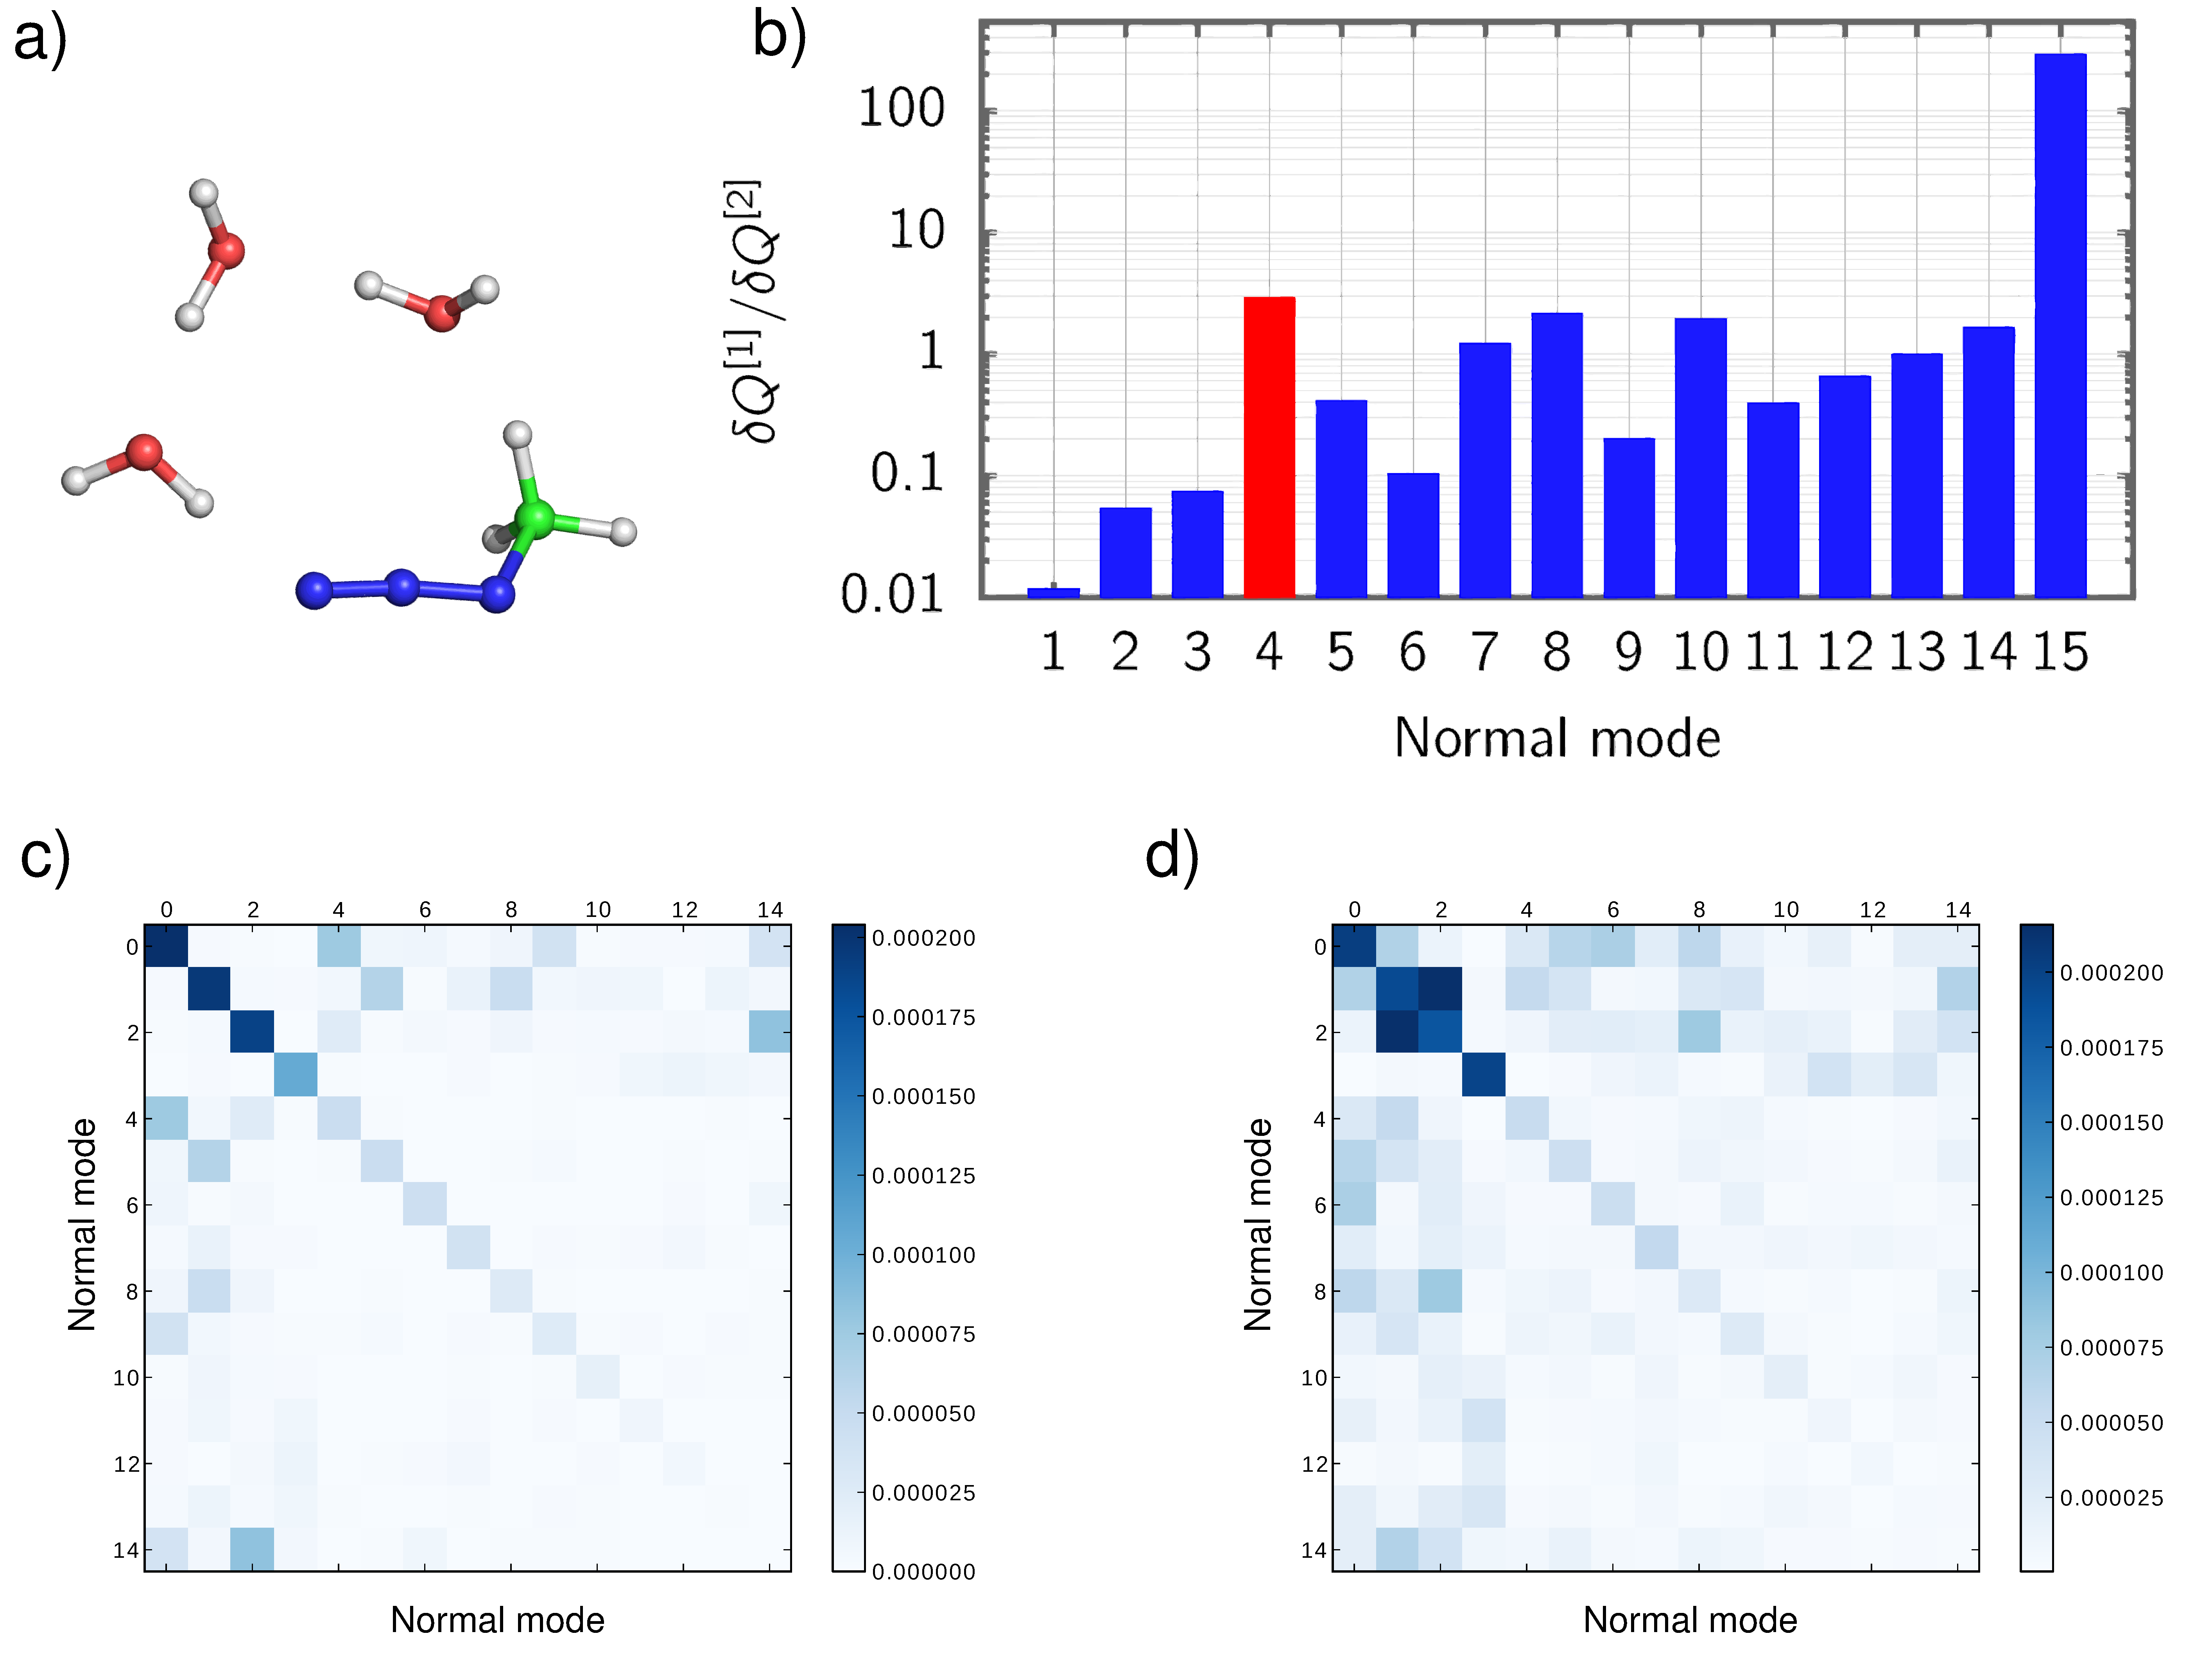
\includegraphics[width=0.9\linewidth]{Fig-men3-dq.eps}
}
\caption{Structural distortions of MeN$_3$ molecule and the resulting vibrational
frequencies calculated by using B3LYP/6-311++G** method. 
a) The structure of a model complex; b) relative differences of the
structural distortions
calculated for each normal mode displacement; c) and d) Hessian matrix in MeN$_3$ gas-phase normal coordinate
space calculated by using approximations `1' and `2' from the main text 
($\delta {\bf Q}^{[1]}$ and $\delta {\bf Q}^{[2]}$ in this Figure, respectively).
Hessian matrices were averaged over 20 model MeN$_3$--(H$_2$O)$_{n=1-10}$ configurations.
\label{f.MeN3.dq}}
\end{figure}
%

In fact, the differences in the vibrational solvatochromisms of NMA and MeN$_3$ are quite significant. 
This is because amide I modes are surprisingly well described by purely Coulombic 
models \citep{Blasiak.Lee.Cho.JCP.2013,Blasiak.Cho.JCP.2014,Blasiak.Cho.JCP.2015}
which is in stark contrast to triple\hyp{}bonded IR probes solvatochromism such as 
CN, NC or N$_3$. \citep{Blasiak.Ritchie.Webb.Cho.PCCP.2016,Maj.Ahn.Blasiak.Kwak.Han.Cho.XXX.2016}
We will discuss this issue in more detail later when the non-Coulombic effects 
are also derived and extensively quantified.

In the examples studied above we considered the frequency of only localised 
normal modes. Nevertheless, when approximation `1'
is used, frequency shifts need to be computed under diagonal Hessian approximation
and it is not possible to study the intramolecular mode mixing process without additional 
modifications of the procedure. Therefore, approximation `2' might be useful when one
wanted to study the solvation\hyp{}induced mode mixing. Nevertheless, this aspect needs to
be investigated in more detail in the future.\footnote{The research presented here is not published yet.}
Moreover, electrostatic model is not working properly for azide IR probes.

\section{Vibrational Transition Dipole\label{s:vibr-trans-dipole}}

Up to that moment, we were considering only the vibrational frequency shifts
but it is also very useful to study the change of the vibrational
transition dipole due to solvation because it contains the critical
information about the changes in the IR absorption intensity.

To a good approximation, vibrational transition dipole is proportional to the dipole derivative 
with respect to the normal coordinate evaluated at the equilibrium geometry.
Therefore, it is sufficient to consider the change in the dipole derivative
upon solvation. In solution we have
%
\begin{equation} \label{e:dipole-solution}
{\BM \mu}({\bf F}) \approx {\BM \mu}_0 + {\BM \alpha}_0 \cdot {\bf F}
\end{equation}
%
and the dipole derivative is
%
\begin{equation} \label{e:dipole-der-solution}
 \frac{\partial{\BM \mu}({\bf F})}{\partial\overline{Q}_j} \Bigg|_{\overline{\bf Q}_{0_A}}
\approx 
 \frac{\partial{\BM \mu}({\bf F})}{\partial Q_j} \Bigg|_{{\bf Q}_{0_A}}
+
\sum_i \frac{\partial^2{\BM \mu}({\bf F})}{\partial Q_j \partial Q_i} \Bigg|_{{\bf Q}_{0_A}}
\left( \overline{Q}_i - Q_i\right)
\end{equation}
%
In the above equations, ${\BM \mu}_0$ and ${\BM \alpha}_0$ denote 
the solute's gas\hyp{}phase dipole moment
and polarizability, respectively.
Thus, by using the results obtained in Eqs.~\eqref{e:struct-dist-cho} 
and \eqref{e:struct-dist-cho-transl},
the difference transition dipole is given by
%
\begin{equation} \label{e:dipole-der-diff-solution}
\frac{\partial{\BM \mu}({\bf F})}{\partial\overline {\bf Q}_j} \Bigg|_{\overline{\bf Q}_{0_A}} -  
 \frac{\partial{\BM \mu}({\bf F}={\bf 0})}{\partial {\bf Q}_j} \Bigg|_{{\bf Q}_{0_A}} \approx
%
\frac{\partial{\BM \alpha}_0}{\partial Q_j} \Bigg|_{{\bf Q}_{0_A}} \cdot {\bf F}
+
\sum_i \frac{U_{0,i}}{M_i\omega_i^2} 
\left\{
\frac{\partial^2{\BM \alpha}_0}{\partial Q_j \partial Q_i} \Bigg|_{{\bf Q}_{0_A}} \cdot {\bf F}
+
\frac{\partial^2{\BM \mu}_0}{\partial Q_j \partial Q_i} \Bigg|_{{\bf Q}_{0_A}}
\right\}
\end{equation}
%
In a limiting case when
the interaction potential is approximated by the multipole expansion from
Eq.~\eqref{e:dmtp}, 
%and with constant $\nabla \phi$ 
%(i.e., $\phi({\bf r}) = {\bf r} \cdot {\bf F} + {\rm const.}$), 
Eq.~\eqref{e:dipole-der-diff-solution} can be recast 
in a simple form
%
\begin{equation} \label{e:dipole-der-diff-solution-field}
 \frac{\partial{\BM \mu}({\bf F})}{\partial\overline {\bf Q}_j} \Bigg|_{\overline{\bf Q}_{0_A}} -  
 \frac{\partial{\BM \mu}({\bf F}={\bf 0})}{\partial {\bf Q}_j} \Bigg|_{{\bf Q}_{0_A}} \cong
%
\left[
\frac{\partial {\BM \alpha}_0}{\partial Q_j} \Bigg|_{{\bf Q}_{0_A}} 
+ 
\sum_i \frac{1}{M_i\omega_i^2} 
\frac{\partial^2 {\BM \mu}_0}{\partial Q_j \partial Q_i} \Bigg|_{{\bf Q}_{0_A}}
\otimes
\frac{\partial {\BM \mu}_0}{\partial Q_i} \Bigg|_{{\bf Q}_{0_A}}
\right] 
\cdot {\bf F}
\end{equation}
%
in which we neglected the contributions of the polarizability second derivatives.

Note that the above discussion refers to the case
in which electric field is uniform in space. 
In the case when the electric field has a notable
gradients around the vibrational chromophore
the dipole\hyp{}dipole polarizability approximation from Eq.~\eqref{e:dipole-solution} 
is not sufficient. 

There are several ways to tackle the problem of non\hyp{}uniform
electric field.
One of them is to
add the quadrupole polarizabilities to Eq.~\eqref{e:dipole-solution} 
and obtain, for example, the contributions
of the kind $\frac{1}{3} \frac{\partial{\bf A}_0}{\partial Q_j} \big|_{{\bf Q}_{0_A}} \cdot {\BM \nabla}{\bf F}$ 
where ${\bf A}_0$ is the quadrupole-dipole polarizability. Another way is to use
charge\hyp{}response kernel approach in which
the first term in Eq.~\eqref{e:dipole-der-diff-solution} should be generalised 
to the following form \citep{Cho.JCP.2009}
%
\begin{equation} \label{e:trans-dip-cho-pot-ind-effect}
\left( \frac{\partial{\BM \alpha}_0}{\partial Q_j} \Bigg|_{{\bf Q}_{0_A}} \cdot {\bf F} \right)
\;\longrightarrow\;
2\int_V {\rm d}\;{\bf r} \int_V    {\rm d}\;{\bf r}' \; 
\left\{
\frac{\partial \kappa({\bf r},{\bf r}')}{\partial Q_j} \Bigg|_{{\bf Q}_{0_A}} {\bf r} \phi({\bf r}')
\right\}
%
\end{equation}
%
where $\kappa({\bf r},{\bf r}')$ denotes the charge response kernel
of solute. Analogously,
%
\begin{equation} \label{e:trans-dip-cho-pot-ind-effect-quadratic}
\left( \frac{\partial^2{\BM \alpha}_0}{\partial Q_j \partial Q_i} \Bigg|_{{\bf Q}_{0_A}} \cdot {\bf F} \right)
\;\longrightarrow\;
2\int_V {\rm d}\;{\bf r} \int_V    {\rm d}\;{\bf r}' \; 
\left\{
\frac{\partial^2 \kappa({\bf r},{\bf r}')}{\partial Q_j \partial Q_i} \Bigg|_{{\bf Q}_{0_A}} {\bf r} \phi({\bf r}')
\right\}
%
\end{equation}
%
Perhaps the most practical way is to employ the distributed
polarizabilities, i.e., do the replacement ${\BM \alpha}_0\rightarrow\sum_a{\BM \alpha}_{a,0}$
where the $a$th polarizable site is located at ${\bf r}_a$. 
In this scenario, the difference transition dipole 
is simply expressed as
%
\begin{multline}[box=\widebox] \label{e:dipole-der-diff-solution-distributed}
\frac{\partial{\BM \mu}({\bf F})}{\partial\overline {\bf Q}_j} \Bigg|_{\overline{\bf Q}_{0_A}} -  
 \frac{\partial{\BM \mu}({\bf F}={\bf 0})}{\partial {\bf Q}_j} \Bigg|_{{\bf Q}_{0_A}} \approx
%
\sum_a \left\{
\frac{\partial{\BM \alpha}_{a,0}}{\partial Q_j} \Bigg|_{{\bf Q}_{0_A}} 
+
\sum_i \frac{U_{0,i}}{M_i\omega_i^2} 
%
\frac{\partial^2{\BM \alpha}_{a,0}}{\partial Q_j \partial Q_i} \Bigg|_{{\bf Q}_{0_A}} 
\right\} \cdot {\bf F}({\bf r}_a) \\
+
\sum_i \frac{U_{0,i}}{M_i\omega_i^2}
\frac{\partial^2{\BM \mu}_0}{\partial Q_j \partial Q_i} \Bigg|_{{\bf Q}_{0_A}}
%
\qquad\qquad\qquad\qquad\qquad\qquad
\end{multline}
%
In the above expression, electric field is determined at
various polarizable sites which we denote here as ${\bf F}({\bf r}_a)$.

The theory presented in this Section is absolutely general 
for any kind of the solute\hyp{}solvent
interaction potential. Later on, we shall discuss the origins of the
vibrational frequency shifts and transition dipole differences
upon solvation.


\section{Summary}

In this Chapter, we have discussed the first\hyp{}principles
vibrational solvatochromism theories of Buckingham and Cho which,
although originate from different starting points, lead to the same results.
Thus, the vibrational solvatochromic frequency shift of a spatially localised 
IR probe normal mode can be described by Eq.~\eqref{e:buckingham-2st-order-total-fund}
which is second\hyp{}order in the perturbation of the isolated harmonic oscillator Hamiltonian.
This model i) assumes the first\hyp{}order structural distortion of solute, which takes 
into account only the solute\hyp{}solvent interaction potential and neglects
solute's anharmonicity, as well as ii) considers the solvation\hyp{}induced change of the diagonal
Hessian matrix elements only, while the off\hyp{}diagonal elements
contribute only to the mode mixing in the limit of small Hessian perturbation. 
Therefore, we referred to this theory
as to the \emph{weak coupling approximation} (WCA). The theory reproduces well the frequency shifts of
simple localised vibrations as well as structural distortions
when the exact solute\hyp{}solvent interaction potential
is employed. However, since the WCA cannot describe the normal modes
which are delocalized over many atoms, the approach of considering
the Hessian matrix proposed by Cho in Eq.~\eqref{e:force-const-cho} is necessary. 
In that case, particular caution should be made because the structural
distortion estimation is not well researched up to that moment. If the
first-order approximation from Eq.~\eqref{e:struct-dist-cho} failed in some cases, the results 
derived in Sec.~\ref{s:str-dist-general-discussion} might become useful.

\printbibliography[heading=subbibintoc,title={References}]
\end{refsection}

% === Chapter 4 ===
\begin{refsection}
\chapter{Rigorous Models of Vibrational Solvatochromism \label{c:my-model}}

Although the theory of the vibrational solvatochromism
was developed before, it involved the total solute\hyp{}solvent
intermolecular potential which is an extremely complicated function
of molecular properties.
Therefore, it is important to find explicit 
expressions that link the vibrational solvatochromism
to the particular interaction phenomenon.
Only then it is possible to obtain a robust model
that can be further applied for condensed phases. 
In this Chapter, we develop the rigorous first\hyp{}principles
theory of the vibrational frequency shifts and transition
dipole changes.
Due to historical reasons, we first develop a model in terms
of the implicit theories of solvation in which solute's molecular
environment is approximated by a continuum. 
Next, we derive the explicit theory based on five fundamental interactions
between molecules that can be found in nature: Coulombic, 
exchange\hyp{}repulsion, induction, dispersion and charge\hyp{}transfer.
Finally, we develop an approximate approach to
to estimating the long\hyp{}range corrections to the vibrational
frequency shifts when the solution extends to infinity. 

The considerable
part of this Chapter is based on the Hartree\hyp{}Fock theory. \citep{Roothaan.RevModPhys.1951}
Readers who
are not familiar with the molecular orbital approximation and the mean\hyp{}field
treatment of the Schr{\"o}dinger equation are strongly urged to read first the
Chapters 2 and 3 of an excellent book by Szabo and Ostlund \citep{Szabo.Ostlund.ModernQuantumChemistry.1996}
It is also recommended to become familiar with the basic schemes of implementation of molecular
integrals which can be found in Ref. \citep{Cook.HandbookOfComputationalQuantumChemistry.2005}

\section{Implicit Model: Coulombic and Induction Effects\label{s:implicit-model}}

At the heart of the foundations of our knowledge about the 
physical chemistry of liquids and solutions are the \emph{continuum}
models of Onsager, Kirkwood and Fr{\"o}hlich. They
provided invaluable insight into the solvation
process from statistical thermodynamical point of view, linking
the microscopic characteristics of molecular species
with the macroscopic representatives of liquids
such as density, dielectric constant or refractive index.
Despite they cannot capture all the intermolecular
interactions effects rigorously, they do often provide a surprisingly 
correct
description of various observables in solution.
Therefore, it is instructive to study continuum models of solvation
in terms of the vibrational solvatochromism since they 
are still used by some researchers to relate macroscopic
solvent properties with molecular vibrational characteristics
in aprotic solvents.

As the simplest case let us consider the situation
in which the neutral solute molecule with the permanent gas\hyp{}phase 
dipole moment ${\BM \mu}_0$
is placed inside a spherical cavity of radius $a$, i.e., the 
Onsager model. 
%Note that
%for our purpose the cavity need to be quite large. Therefore 
%we can safely neglect other than dipole\hyp{}dipole interactions
%and consider the Onsager model of solvation.
In such a case, the solvation (interaction) energy is given as
%
\begin{equation} \label{e:esol-onsager}
 U^{\rm Sol}(\varepsilon, {\bf Q}) =
 -\frac{1}{2} {\BM \mu}(\varepsilon, {\bf Q}) \cdot {\bf F}^{\rm Ons}
\end{equation}
%
where the Onsager reaction (electric) field acting on the solute molecule
is
%
\begin{equation} \label{e:fons}
  {\bf F}^{\rm Ons} = \frac{2(\varepsilon-1)(n^2+1)}{3a^3(2\varepsilon+n^2)} {\BM \mu}(\varepsilon, {\bf Q})
 = g(a,\varepsilon) {\BM \mu}(\varepsilon, {\bf Q})
\end{equation}
%
In the above equations, ${\BM \mu}(\varepsilon, {\bf Q})$ 
is the total solute's (gas\hyp{}phase and induced) dipole moment.
It is straightforward to write down the expression for the
vibrational frequency shift as
%
\begin{equation} \label{e:dw-ons-gen}
  \Delta\omega_j(\varepsilon, {\bf Q}) = \hat{F}_j \left[ U^{\rm Sol}(\varepsilon, {\bf Q}) \right]
\end{equation}
%
where $\hat{F}_j$ is the vibrational solvatochromic frequency shift 
operator from Eq.~\eqref{e:dw-fea-fma}.

To calculate the solvatochromic vibrational frequency shift
using solute's gas\hyp{}phase properties it is necessary to expand
the dipole moment into a power series with respect to the two perturbations,
i.e., structural distortion and the Onsager electric field. Considering the first
four terms in the Taylor expansion of ${\BM \mu}(\varepsilon, {\bf Q})$ one gets
%
\begin{equation} \label{e:mu-qf}
 {\BM \mu}(\varepsilon, {\bf Q}) \approx 
 {\BM \mu}_0 + \fderiv{{\BM \mu}}{\bf F}\Bigg|_{0}  \cdot {\bf F}^{\rm Ons}
 + \sum_i \fderiv{{\BM \mu}}{Q_i}\Bigg|_{0} \delta Q_i 
 + \sum_i \sderivd{{\BM \mu}}{{\bf F}}{Q_i}\Bigg|_{0} \cdot {\bf F}^{\rm Ons} \delta Q_i
\end{equation}
%
where the subscript $0$ denotes that the derivatives are evaluated in the gas phase,
i.e., ${\bf F}={\bf 0}$ and $\delta Q_i=0$. Computation of the solute dipole
moment is not so easy since the relaxation process of the electronic wavefunction
and molecular structure has to be taken into account. This can 
be introduced in a one\hyp{}electron Hamiltonian in the Schr{\"o}dinger equation
or its approximate form. However, this is still relatively costly. Beneath
we present the approximate method of taking into account
this relaxation process basing solely on the solute's gas\hyp{}phase properties.

\subsection{Rigid Molecule Approximation}

Let us first consider the case when we neglect structural
relaxation due to the reaction field and focus only
on the electronic charge density redistribution. In such a case,
%
\begin{equation}
 {\BM \mu}(\varepsilon, {\bf Q}) \approx 
 {\BM \mu}_0 + {\BM \alpha}_0  \cdot {\bf F}^{\rm Ons}
\end{equation}
%
where the dipole\hyp{}dipole gas\hyp{}phase polarizability is
%
\begin{equation}
{\BM \alpha}_0  = \fderiv{{\BM \mu}}{\bf F}\Bigg|_{0}
\end{equation}
%
Then, the Onsager reaction field can be approximately written as
%
\begin{equation}
{\bf F}^{\rm Ons} \approx g(a,\varepsilon) {\bf B} \cdot {\BM \mu}_0
\end{equation}
%
with the auxiliary matrix given as follows
%
\begin{equation}
{\bf B} = \left( {\bf 1} - g(a,\varepsilon){\BM \alpha}_0 \right)^{-1}
\end{equation}
%
Thus, the resulting solvation energy can be recast in the form
that depends only on gas\hyp{}phase solute properties:
%
\begin{equation} \label{e:ons-e-sol-init}
U^{\rm Sol}(\varepsilon, \delta{\bf Q}=0) = -\frac{1}{2} {\BM \Phi}(a, \varepsilon) : {\BM \mu}_0 \otimes {\BM \mu}_0
\end{equation}
%
where the ${\BM \Phi}(a, \varepsilon)$ tensor is defined as
%
\begin{equation}
{\BM \Phi}(a, \varepsilon) = g(a,\varepsilon) {\bf B} + g^2(a,\varepsilon) {\bf B} {\BM \alpha}_0 {\bf B}
\end{equation}
%
Now, applying the vibrational solvatochromic frequency shift
operator to this solvation energy,
we find that the frequency shift is
%
\begin{equation} \label{e:dw-ons-working-form}
\Delta\omega_j(\varepsilon, \delta{\bf Q}=0) = \frac{1}{4M_j\omega_j}
\left\{ \sum_i \frac{g_{ijj}}{M_i\omega_i^2}S_i - K_j \right\}
\end{equation}
%
where the coefficients are given as
%
\begin{subequations}
 \begin{align}
  S_i &= \fderiv{{\BM \Phi}}{Q_i} : {\BM \mu}_0 \otimes {\BM \mu}_0 
           + 2{\BM \Phi} : \fderiv{{\BM \mu}_0}{Q_i} \otimes {\BM \mu}_0 \label{e:ons-si-init}\\
  K_j &= \sderiv{{\BM \Phi}}{Q_j} : {\BM \mu}_0 \otimes {\BM \mu}_0
           + 2{\BM \Phi} : \left[ \sderiv{{\BM \mu}_0}{Q_j} \otimes {\BM \mu}_0 
           +  \fderiv{{\BM \mu}_0}{Q_j} \otimes \fderiv{{\BM \mu}_0}{Q_j} \right] 
           + 4\fderiv{{\BM \Phi}}{Q_j} : \fderiv{{\BM \mu}_0}{Q_j} \otimes {\BM \mu}_0  \label{e:ons-ki-init}
 \end{align}
\end{subequations}
%
Note that ${\BM \Phi}$ is symmetric.  

\subsection{Structural Distortion Effect: Iterative Method}

Now, using Eq.~\eqref{e:struct-dist-cho}
we can estimate the structural distortion due to relaxation 
in the first approximation as
%
\begin{equation} \label{e:ons-dq-init}
\delta Q_i \approx \frac{S_i}{2M_i\omega_i^2}
\end{equation}
%
Thus, it becomes possible to iteratively take into account 
the structural distortion effects for the solute's permanent
dipole moment evaluation, which directly influences the 
frequency shift via Eqs.~\eqref{e:esol-onsager}, 
\eqref{e:dw-ons-gen} and \eqref{e:mu-qf}.

When $\hat{F}_j$ acts on the full solvation energy 
the vibrational frequency shift has the same form as 
in Eq.~\eqref{e:dw-ons-working-form}
but the $S_i$ and $K_j$ coefficients are now different:
%
\begin{subequations}
 \begin{align}
  S_i &= \fderiv{{\BM \mu}(\varepsilon,{\bf Q})}{Q_i} \cdot {\bf F}^{\rm Ons}
           + {\BM \mu}(\varepsilon,{\bf Q}) \cdot \fderiv{{\bf F}^{\rm Ons}}{Q_i}
        \label{e:ons-si-iter}  \\
  K_j &= \left[ 
             \sderiv{{\BM \mu}_0}{Q_j}  
        + 2 \fderiv{{\BM \alpha}_0}{Q_j}  \cdot \fderiv{{\bf F}^{\rm Ons}}{Q_j}
         \right] \cdot {\bf F}^{\rm Ons}
         + 2\fderiv{{\BM \mu}(\varepsilon,{\bf Q})}{Q_j} \cdot \fderiv{{\bf F}^{\rm Ons}}{Q_j}
        \label{e:ons-ki-iter}
 \end{align} % i have multiplied K_j by 2
\end{subequations}
%
Analogously, the structural distortion is 
$\delta Q_i=S_i/2M_i\omega_i^2$.
One of the necessary derivatives are directly found to be
%
\begin{multline} \label{e:mu-qf-derivative}
\fderiv{{\BM \mu}(\varepsilon,{\bf Q})}{Q_j} =
\fderiv{{\BM \mu}_0}{Q_j} + \fderiv{{\BM \alpha}_0}{Q_j}  \cdot {\bf F}^{\rm Ons}
+ \sum_i \sderivd{{\BM \mu}_0}{Q_j}{Q_i} \delta Q_i 
+ \sum_i \sderivd{{\BM \alpha}_0}{Q_j}{Q_i} \cdot {\bf F}^{\rm Ons} \delta Q_i \\
+ {\BM \alpha}_0  \cdot \fderiv{{\bf F}^{\rm Ons}}{Q_j} 
+ \sum_i \fderiv{{\BM \alpha}_0}{Q_i} \delta Q_i \cdot \fderiv{{\bf F}^{\rm Ons}}{Q_j} 
\end{multline}
%
Moreover, from Eqs.~\eqref{e:mu-qf}
and \eqref{e:fons} one can easily find that
the Onsager reaction field is given as
%
\begin{equation} \label{e:ons-field}
 {\bf F}^{\rm Ons} = -{\bf A}^{-1} \cdot 
\left[ 
   {\BM \mu}_0 + \sum_i \fderiv{{\BM \mu}_0}{Q_i}\delta Q_i
\right]
\end{equation}
%
where the matrix $\bf A$, which can be viewed as generalised polarizability,
is
%
\begin{equation} \label{e:a-matrix}
{\bf A} = {\BM \alpha}_0 - \frac{1}{g(a,\varepsilon)} {\bf 1}
   + \sum_i \fderiv{{\BM \alpha}_0}{Q_i}\delta Q_i
\end{equation}
%
Thus the derivatives of the Onsager field are found to be
%
\begin{equation} \label{e:ons-field-deriv}
\fderiv{{\bf F}^{\rm Ons}}{Q_j}  = 
- {\bf A}^{-1} 
   \left[ 
       \fderiv{{\BM \mu}_0}{Q_j} 
      + \sum_i \sderivd{{\BM \mu}_0}{Q_j}{Q_i} \delta Q_i 
      - \fderiv{{\bf A}}{Q_j}  {\bf A}^{-1}  
           \left\{ 
               {\BM \mu}_0 + \sum_i \fderiv{{\BM \mu}_0}{Q_i}\delta Q_i
           \right\}
   \right]
\end{equation}
%
where
%
\begin{equation}
  \fderiv{{\bf A}}{Q_j} = \fderiv{{\BM \alpha}_0}{Q_j} 
               + \sum_i \sderivd{{\BM \alpha}_0}{Q_j}{Q_i} \delta Q_i
\end{equation}
%
We are now ready to outline the iterative procedure
to converge $U^{\rm Sol}$ with respect to both electronic
charge density polarization and the structural
relaxation:
%
\begin{itemize}
\item[\textbullet] {\bf Initial Conditions}. 
                        By starting from rigid molecule approximation,
                        precompute the solvation energy from Eq.~\eqref{e:ons-e-sol-init}
                        and the initial structural distortions
                        from Eq.~\eqref{e:ons-dq-init} and 
                        Eq.~\eqref{e:ons-si-init}
\item[\textbullet] {\bf Iterations}. Start the iterative procedure 
                        by recomputing $U^{\rm Sol}$ and $\delta Q_i$
\begin{enumerate}
 \item Calculate Onsager field using Eqs.~\eqref{e:ons-field} and \eqref{e:a-matrix}, 
       and its derivatives from Eq.~\eqref{e:ons-field-deriv}
 \item Calculate dipole moment using Eq.~\eqref{e:mu-qf} 
       and its derivatives from Eq.~\eqref{e:mu-qf-derivative}
 \item Calculate structural distortions from Eq.~\eqref{e:ons-dq-init}
       and Eq.~\eqref{e:ons-si-iter}
 \item Calculate solvation energy using Eq.~\eqref{e:esol-onsager}
 \begin{itemize}
      \item if $\left| U^{\rm Sol}_{\rm old} - U^{\rm Sol}_{\rm new}\right| > \Delta U^{\rm crit}$:
            continue by updating the derivatives of dipole moment and Onsager field
            and going back to the next iteration
      \item else: End. 
 \end{itemize}    
\end{enumerate}
\end{itemize}
%
Once the solvation energy is converged 
(lowered as solute molecule
relaxes from its gas\hyp{}phase geometry) 
up to a chosen criterion $\Delta U^{\rm crit}$
one can readily obtain
the vibrational frequency shift by using Eqs.~\eqref{e:dw-ons-working-form},
\eqref{e:ons-si-iter} and \eqref{e:ons-ki-iter}.

In terms of accuracy, the rigid molecule approximation
provides already a good solvation energies and the frequency shifts
even for small cavity sizes which are simulating the molecular
volume
(see Section~\ref{s:amide-I-onsager}). 
%Therefore, to estimate
%the frequency shift long\hyp{}range correction
%it is sufficient to focus
%on the approximation given in Eq.~\eqref{e:ons-e-sol-init}
%and the resulting vibrational frequency shift.
%This is mostly because, for our purposes, $a$ shall be typically
%large (much larger than the effective radius of the molecular
%charge distribution), and the structural distortion effects can be 
%neglected without significant loss of accuracy.

\subsection{The Nature of Interactions in Onsager Model}

Onsager solvation energy is derived based on solving Poisson
equation for the boundary conditions specified by a point
dipole in a cavity surrounded by continuum dielectric.
Therefore the electrostatic effects that include polarization
energy are treated semi\hyp{}classically.

Let us study the origin of the vibrational frequency shift
within the Onsager model. 
%To obtain the explicit forms of $\Delta\omega_j^{\rm Coul}$
%and $\Delta\omega_j^{\rm Ind}$
%$\widetilde{\Delta\omega}_j^{\rm Coul}$
%and $\widetilde{\Delta\omega}_j^{\rm Ind}$ 
When the structural relaxation effect on solute's dipole moment
is neglected we can rewrite the frequency shift to be
%
\begin{equation} \label{e:f9f9f}
 \Delta\omega_j(\varepsilon, a) \approx 
- \left[ {\BM \mu}_j + \frac{1}{2} {\BM \mu}_j^{\rm Ind} \right] \cdot {\bf F}^{\rm Ons} 
- \frac{1}{2} {\BM \alpha}_j : {\bf F}^{\rm Ons} \otimes {\bf F}^{\rm Ons} 
+ \Delta\omega_j({\bf F})
 = \Delta\omega_j^{\rm Coul} + \Delta\omega_j^{\rm Ind}
\end{equation}
%
where the Coulombic and induction frequency shifts 
are defined as
%
\begin{subequations}
 \begin{align}
   \Delta\omega_j^{\rm Coul}             &= - {\BM \mu}_j \cdot {\bf F}^{\rm Ons} + \Delta\omega_j({\bf F})\\
   \Delta\omega_j^{\rm Ind}              &= - \frac{1}{2} {\BM \mu}_j^{\rm Ind} \cdot {\bf F}^{\rm Ons} 
       - \frac{1}{2} {\BM \alpha}_j : {\bf F}^{\rm Ons} \otimes {\bf F}^{\rm Ons} 
 \end{align}
\end{subequations}
%
The effective gas\hyp{}phase and induced solvatochromic dipoles
are defined as
%
\begin{subequations}
 \begin{align}
   {\BM \mu}_j &= \frac{1}{4M_j\omega_j}
\left[  \sderiv{{\BM\mu}_0}{Q_j}
- \sum_i \frac{g_{ijj}}{M_i\omega_i^2} \fderiv{{\BM\mu}_0}{Q_i}
\right] \\
   {\BM \mu}_j^{\rm Ind} &= \frac{1}{M_j\omega_j} 
\left[ 2 \fderiv{{\bf F}^{\rm Ons}}{Q_j} \cdot \fderiv{{\BM\alpha}_0}{Q_j} - 
   \sum_i \frac{g_{ijj}}{M_i\omega_i^2} \fderiv{{\bf F}^{\rm Ons}}{Q_i} \cdot {\BM\alpha}_0
\right]
 \end{align}
\end{subequations}
%
whereas the solvatochromic polarizability is
%
\begin{equation} 
  {\BM \alpha}_j = - \frac{1}{2M_j\omega_j} 
   \sum_i \frac{g_{ijj}}{M_i\omega_i^2} \fderiv{{\BM\alpha}_0}{Q_i}
\end{equation}
%
In Eq.~\eqref{e:f9f9f}, we separated the ``electric\hyp{}field correction''
term from the Coulombic term due to technical reasons,
%
\begin{equation} 
\Delta\omega_j({\bf F}) = \frac{1}{4M_j\omega_j}
\sum_i \left\{ \frac{g_{ijj}}{M_i\omega_i^2}  {\BM\mu}_0 - 
2\delta_{ij} \left(
\fderiv{{\BM\mu}_0}{Q_i}
+ 
 {\BM\alpha}_0 \cdot \fderiv{{\bf F}^{\rm Ons}}{Q_i}
\right)
\right\} \cdot \fderiv{{\bf F}^{\rm Ons}}{Q_i}
\end{equation}
%
This contribution depends on the electric field derivatives with respect to the vibrational
coordinate while it does not involve the electric field itself. Therefore
it cannot be written in a way that is analogous
to the conventional multipole expansion of interaction energy 
in which dipoles (permanent and induced) interact with electric fields.

As can be seen, Onsager model includes semi classically
Coulombic and induction energies. However, it cannot
deal with dispersion effects that are fully quantum mechanical
in nature. Moreover,
%It is interesting to note the straightforward
%similarity of the above equations to the corresponding
%contributions in the descrete model of vibrational
%solvatochromism discussed in previous Sections.
Onsager model (and any other continuum approach) 
is incapable of modelling
explicit solvation effects such as molecular collisions
and specific interactions. Therefore, its significance
lies mostly in the concept of the non\hyp{}specific
vibrational frequency shift (due to electrostatic
interactions) and should not be used for quantitative
calculations, especially when specific interactions such as
hydrogen bonds exist between solute and its molecular environment.


\section{Explicit Model: Coarse-Graining\label{s:vibr-solv-explicit-models}}

We focus now on the treatment of each molecule
explicitly which enables one to take into account
the intricate scenarios of intermolecular contacts
starting from random collisions, weak van der Waals
forces to more directional, specific interactions
such as strong electrostatic forces, H-bonding and
$\pi$-interactions.

\subsection{Coulombic Effects\label{s:dw-coul}}

In the first\hyp{}order of polarization perturbation
theory\footnote{i.e., in the long\hyp{}distance limit 
where the wavefunction overlap vanishes. In such a case the
exchange and charge\hyp{}penetration effects 
between solute and solvent molecules can be safely ignored.}, 
the intermolecular interaction potential
can be understood as a Coulombic interaction
of unperturbed solute and solvent molecules (i.e., 
as if they were isolated). \citep{Jeziorski.Moszynski.Szalewicz.ChemRev.1994,
Stone.TheTheoryOfIntermolecularForces.1996}
That is
%
\begin{equation} \label{e:eint-1}
U^{(1)} = 
\langle 0_A0_B \lvert \mathscr{V}_{AB} \rvert 0_A0_B \rangle 
\end{equation}
%
Here, $\mathscr{V}_{AB}$ is the solute\hyp{}solvent
interaction potential defined as $\mathscr{V}_{AB}\equiv\mathscr{H}_{AB} - \mathscr{H}_{0_A} - \mathscr{H}_{0_B} $,
and $\vert 0_A0_B \rangle \cong \vert 0_A \rangle \otimes \vert 0_B \rangle$
and $\vert mn \rangle \cong \vert m \rangle \otimes \vert n \rangle$
represent the electronic ground state and excited states
of the $AB$ complex, respectively. The isolated electronic states of monomers $A$
and $B$ are determined by the time\hyp{}independent Schr{\"o}dinger
equations
%
\begin{subequations}
 \begin{align}
  \mathscr{H}_{0_A} \vert m \rangle &= \hbar \omega_m \vert m \rangle \\
  \mathscr{H}_{0_B} \vert n \rangle &= \hbar \omega_n \vert n \rangle
 \end{align}
\end{subequations}
%
Then it becomes legitimate to model the electrostatic interaction
energy by considering the distributed multipole expansion of electron
charge density distributions \citep{Stone.TheTheoryOfIntermolecularForces.1996}
which is given in Eq.~\eqref{e:dmtp}. Analogously,
the electrostatic potential and its gradients
can be also multipole\hyp{}expanded as follows
%
\begin{equation} \label{e:potential-gradients}
\underbrace{\nabla \otimes \cdots \otimes \nabla}_{r} \phi({\bf r}_x) = 
\sum_y \left[ 
{\bf T}^{(r)} q_y - {\bf T}^{(r+1)} \cdot {\BM \upmu}_y + 
 \frac{1}{3} {\bf T}^{(r+2)} : {\BM \Theta}_y - 
\frac{1}{15} {\bf T}^{(r+3)} : {\BM \Omega}_y + \ldots
\right]
\end{equation}
%
where 
${\BM \nabla} \equiv \sum_{\zeta}^{x,y,z} \hat{\bf i}_\zeta \frac{\partial}{\partial \zeta_x}$, 
$y$ runs over all solvent electrostatic distributed sites
and ${\bf T}^{(r)}$ are the so called interaction tensors of rank $r$ which are defined as follows
%
\begin{subequations}
\label{e:interaction-tensors}
\begin{align}
  T^{(0)} &= \frac{1}{\rvert {\bf r}_{xy} \lvert}  \label{e:interaction-tensors-1} \\
  T^{(1)}_\alpha &=-\frac{{\bf r}_{xy;\alpha}}{\rvert {\bf r}_{xy} \lvert^3}  \label{e:interaction-tensors-2} \\
  T^{(2)}_{\alpha\beta} &=3\frac{{\bf r}_{xy;\alpha} {\bf r}_{xy;\beta} }{\rvert {\bf r}_{xy} \lvert^5}  
      - \frac{\delta_{\alpha\beta}}{\rvert {\bf r}_{xy} \lvert^3}             \label{e:interaction-tensors-3} \\
  T^{(3)}_{\alpha\beta\gamma} &= -15 
         \frac{{\bf r}_{xy;\alpha} {\bf r}_{xy;\beta} {\bf r}_{xy;\gamma} }{\rvert {\bf r}_{xy} \lvert^7}
                  +3 \frac{{\bf r}_{xy;\alpha} \delta_{\beta\gamma}+
                           {\bf r}_{xy;\beta}  \delta_{\alpha\gamma}+
                           {\bf r}_{xy;\gamma} \delta_{\alpha\beta}}{\rvert {\bf r}_{xy} \lvert^5} \label{e:interaction-tensors-4}
\end{align}
\end{subequations}
%
with ${\bf r}_{xy} \equiv {\bf r}_x - {\bf r}_y$.

The solvatochromic multipole series expansion given in Eq.~\eqref{e:dmtp-sol}
is approximate because it neglects the change of the electrostatic
potential when the vibration occurs. Here we re\hyp{}derive the 
expression for the frequency shift with explicit inclusion of derivatives
of $\phi$. The first and second derivatives of the Coulombic
electrostatic energy can be expressed as follows \citep{Blasiak.Cho.JCP.2014}:
%
\begin{multline} \label{x:726439}
 \fderiv{U^{\rm Coul}}{Q_i} =
%
\sum_x 
\Bigg[ 
  \fderiv{q_x}{Q_i} \phi({\bf r}_x) + 
  \fderiv{{\BM \upmu}_x}{Q_i} \cdot {\BM \nabla} \phi({\bf r}_x) + \frac{1}{3}  
  \fderiv{{\BM \Theta}_x}{Q_i} : {\BM \nabla}\otimes{\BM \nabla} \phi({\bf r}_x) \\ + \frac{1}{15}   
  \fderiv{{\BM \Omega}_x}{Q_i} \vdots {\BM \nabla}\otimes{\BM \nabla}\otimes{\BM \nabla} \phi({\bf r}_x) + \ldots 
\Bigg] 
%
+
%
\sum_x 
\Bigg[ 
  q_x \fderiv{\phi({\bf r}_x)}{Q_i} + 
  {\BM \upmu}_x \cdot \fderiv{{\BM \nabla} \phi({\bf r}_x)}{Q_i} \\ + \frac{1}{3} 
  {\BM \Theta}_x : \fderiv{{\BM \nabla}\otimes{\BM \nabla} \phi({\bf r}_x)}{Q_i} + \frac{1}{15}
  {\BM \Omega}_x \vdots \fderiv{{\BM \nabla}\otimes{\BM \nabla}\otimes{\BM \nabla} \phi({\bf r}_x)}{Q_i} + \ldots 
\Bigg]
\end{multline}
%
and
%
\begin{multline} \label{x:726440}
 \sderiv{U^{\rm Coul}}{Q_i} =
%
\sum_x 
\Bigg[ 
  \sderiv{q_x}{Q_i} \phi({\bf r}_x) + 
  \sderiv{{\BM \upmu}_x}{Q_i} \cdot {\BM \nabla} \phi({\bf r}_x) + \frac{1}{3}  
  \sderiv{{\BM \Theta}_x}{Q_i} : {\BM \nabla}\otimes{\BM \nabla} \phi({\bf r}_x) \\ + \frac{1}{15}   
  \sderiv{{\BM \Omega}_x}{Q_i} \vdots {\BM \nabla}\otimes{\BM \nabla}\otimes{\BM \nabla} \phi({\bf r}_x) + \ldots 
\Bigg] 
%
+
%
\sum_x 
\Bigg[ 
  q_x \sderiv{\phi({\bf r}_x)}{Q_i} + 
  {\BM \upmu}_x \cdot \sderiv{{\BM \nabla} \phi({\bf r}_x)}{Q_i} \\ + \frac{1}{3} 
  {\BM \Theta}_x : \sderiv{{\BM \nabla}\otimes{\BM \nabla} \phi({\bf r}_x)}{Q_i} + \frac{1}{15}
  {\BM \Omega}_x \vdots \sderiv{{\BM \nabla}\otimes{\BM \nabla}\otimes{\BM \nabla} \phi({\bf r}_x)}{Q_i} + \ldots
\\
%
+2\fderiv{q_x}{Q_i} \fderiv{\phi({\bf r}_x)}{Q_i} 
+2\fderiv{{\BM \upmu}_x}{Q_i} \cdot \fderiv{{\BM \nabla} \phi({\bf r}_x)}{Q_i}
+ \frac{2}{3}  
  \fderiv{{\BM \Theta}_x}{Q_i} : \fderiv{{\BM \nabla}\otimes{\BM \nabla} \phi({\bf r}_x)}{Q_i} \\
+ \frac{2}{15}   
  \fderiv{{\BM \Omega}_x}{Q_i} \vdots \fderiv{{\BM \nabla}\otimes{\BM \nabla}\otimes{\BM \nabla} \phi({\bf r}_x)}{Q_i}
+ \ldots
\Bigg]
\end{multline}
%
where, for the sake of notational simplicity, 
it is assumed that the derivatives are to be evaluated at
solute's gas phase equilibrium geometry.

In the previous studies only the first summation terms in 
Eqs.~\eqref{x:726439} and \eqref{x:726440} were taken into account because 
they were assumed to be the dominant contributions. To evaluate the
magnitudes of all the other remaining terms, one has to calculate
the derivatives of electrostatic potential (and its spatial gradients)
with respect to the normal coordinate. Rewriting the differential 
operators and using the chain rule, we can simplify the
derivative operators in the following way
%
\begin{subequations}  \label{e:deriv-operators}
\begin{align}
\fderiv{}{Q_i} &= \sum_m \fderiv{r_m}{Q_i}\fderiv{}{r_m} 
     \approx \sum_{m\in x} \fderiv{r_m}{Q_i}\fderiv{}{r_m} 
     = {\bf L}_x^{(i)} \cdot {\BM \nabla}_x      \label{e:deriv-operators-1} \\
\sderiv{}{Q_i} &= \sum_{mn} \fderiv{r_m}{Q_i}\fderiv{r_n}{Q_i}\sderivd{}{r_m}{r_n} 
     \approx \sum_{m\in x}\sum_{n\in x} \fderiv{r_m}{Q_i}\fderiv{r_n}{Q_i}\sderivd{}{r_m}{r_n} 
     = {\bf L}_x^{(i)} \otimes {\bf L}_x^{(i)} : {\BM \nabla}_x\otimes{\BM \nabla}_x  \label{e:deriv-operators-2}
\end{align}
\end{subequations}
%
where $n$ and $m$ represent the Cartesian coordinates of solute
atomic centres and ${\bf L}_x^{(i)}$ denotes the mass\hyp{}weighted
eigenvector referring to the motion of atom $x$ along $Q_i$
(see Appendix~\ref{asec:vibranal} for more details on how to obtain these vectors).
In the above derivations we assumed that the change of the electrostatic
potential due to the displacement along the normal coordinate is, 
to a good approximation, local, that is to say, only the change of the
atomic position ${\bf r}_x$ is important for which electrostatic potential 
is evaluated. This is equivalent to neglecting the intramolecular induction
effects.

Inserting Eqs.~\eqref{e:deriv-operators-1} and ~\eqref{e:deriv-operators-2}
into Eqs.~\eqref{x:726439} and ~\eqref{x:726440} and properly 
grouping terms with the same characters, we obtain
the first and the second derivatives of the intermolecular interaction
potential, which are associated with each multipole moment, i.e.,
%
\begin{subequations}  \label{e:f-terms}
\begin{align}
 U_i^{(q)}          &= \sum_x 
  \left[ \fderiv{q_x}{Q_i} \phi({\bf r}_x) 
 + q_x {\bf L}_x^{(i)} \cdot {\BM \nabla} \phi({\bf r}_x) \right]       
                                                                \label{e:f-terms-1} \\
 U_i^{(\BM\upmu)}     &= \sum_x  
  \left[ \fderiv{{\BM \upmu}_x}{Q_i} \cdot {\BM \nabla}\phi({\bf r}_x) 
 + {\BM \upmu}_x \otimes {\bf L}_x^{(i)} : {\BM \nabla}\otimes{\BM \nabla} \phi({\bf r}_x) \right]     
                                                                \label{e:f-terms-2} \\
 U_i^{(\BM\Theta)}  &= \frac{1}{3} \sum_x  
  \left[ \fderiv{{\BM \Theta}_x}{Q_i} : {\BM \nabla}\otimes{\BM \nabla}\phi({\bf r}_x) 
 + {\BM \Theta}_x \otimes {\bf L}_x^{(i)} : {\BM \nabla}\otimes{\BM \nabla}\otimes{\BM \nabla} \phi({\bf r}_x) \right]      
                                                                \label{e:f-terms-3} \\
 U_i^{(\BM\Omega)}  &= \frac{1}{15} \sum_x      
  \fderiv{{\BM \Omega}_x}{Q_i} \vdots {\BM \nabla}\otimes{\BM \nabla}\otimes{\BM \nabla}\phi({\bf r}_x)  
                                                                \label{e:f-terms-4} 
\end{align}
\end{subequations}
%
and
%
\begin{subequations}  \label{e:k-terms}
\begin{align}
 U_{jj}^{(q)}          &= \sum_x   
    \left[ \sderiv{q_x}{Q_j} \phi({\bf r}_x) 
    + 2 \fderiv{q_x}{Q_j} {\bf L}_x^{(j)} \cdot {\BM \nabla} \phi({\bf r}_x) 
    + q_x {\BM \nabla}\otimes{\BM \nabla} \phi({\bf r}_x) : {\bf L}_x^{(j)} \otimes {\bf L}_x^{(j)} \right]     \label{e:k-terms-1} \\
%
 U_{jj}^{(\BM\upmu)}     &= \sum_x  
    \left[ \sderiv{{\BM \upmu}_x}{Q_j} \phi({\bf r}_x) 
    + 2 \fderiv{{\BM \upmu}_x}{Q_j} \otimes {\bf L}_x^{(j)} : {\BM \nabla}\otimes{\BM \nabla} \phi({\bf r}_x) 
    + {\BM \upmu}_x 
    \cdot {\BM \nabla}\otimes{\BM \nabla}\otimes{\BM \nabla} \phi({\bf r}_x) \vdots {\bf L}_x^{(j)} \otimes {\bf L}_x^{(j)} \right]      
    \label{e:k-terms-2} \\
%
 U_{jj}^{(\BM\Theta)}  &= \frac{1}{3} \sum_x  
    \left[ \sderiv{{\BM \Theta}_x}{Q_j} \phi({\bf r}_x) 
    + 2 \fderiv{{\BM \Theta}_x}{Q_j} \otimes {\bf L}_x^{(j)} \vdots 
              {\BM \nabla}\otimes{\BM \nabla}\otimes{\BM \nabla} \phi({\bf r}_x)  \right]      
    \label{e:k-terms-3} \\
%
 U_{jj}^{(\BM\Omega)}  &= \frac{1}{15} \sum_x \sderiv{{\BM \Omega}_x}{Q_j} \phi({\bf r}_x)       \label{e:k-terms-4}
\end{align}
\end{subequations}
%
For clarity, only tensors whose rank is less than four are kept in the above summations.
The formulae in Eqs.~\eqref{e:f-terms} and \eqref{e:k-terms} look rather formidable,
especially due to the fact that the potentials and their 
gradients\footnote{in the current implementation up to third rank}
have to be computed from Eq.~\eqref{e:potential-gradients}
which is also a multipole expansion. Therefore,
the electrostatic\hyp{}potential\hyp{}corrected frequency shift
becomes
%
\begin{equation} \label{e:dw-solefp-coul}
\Delta \omega_j^{\rm Coul} = \Delta \omega_j^{\rm SolDMA} + \Delta\omega_j({\partial\phi}) 
\end{equation}
%
where $\Delta \omega_j^{\rm SolDMA}$ is equal to the distributed multipole analysis (DMA)
expansion approximating the Coulombic frequency shift given in Eq.~\eqref{e:dmtp-sol} whereas
%
\begin{equation} \label{e:dw-solefp-coul-correction}
\Delta\omega_j({\partial\phi})  = -\frac{1}{2M_j\omega_j}
\sum_{x \in A}\sum_{y \in B}
\Big[
\sum_i  \frac{g_{ijj}}{M_i\omega_i^2} \sum_{r^{-n} \textrm{ terms} } U_i^{xy} - \sum_{r^{-n} \textrm{ terms} } U_{jj}^{xy}
\Big]
\end{equation}
%
The resulting terms $U_i^{xy}$ and $U_{jj}^{xy}$ in Eq.~\eqref{e:dw-solefp-coul-correction}
have various asymptotic distance dependencies (denoted above as $r^{-n}$
where $r$ is the distance between the distributed multipole centres).
The explicit formulae
that can be directly implemented into a computer code
are listed in Appendix~\ref{a:fk-terms} according to $n$. 
Note that only terms with $n\ge 2$ contribute (i.e., charge-dipole
like terms) because of the differentiation operator.

Before we move to analyse the non\hyp{}Coulombic frequency shifts, two cautionary remarks
on the Coulomb frequency shift correction from Eq.~\eqref{e:dw-solefp-coul-correction} should be made.
First, note that, while $\Delta \omega_j^{\rm SolDMA}$ can be computed from the
solvatochromic multipoles that can be stored in a generalised object
describing a molecule, $\Delta\omega_j({\partial\phi})$ requires 
additionally other quantities that cannot be incorporated
into the definition of the solvatochromic multipole due to the directional
terms coupling solute and solvent distances. Therefore,
the evaluation of the frequency shift including electrostatic potential
correction complicates the implementation (additionally, multipole moments
and their first derivatives with respect to all the normal coordinates need 
to be stored as well). However, it is mostly the case
that $\Delta\omega_j({\partial\phi})$ is much smaller than $\Delta \omega_j^{\rm SolDMA}$
so under certain circumstances the former contribution could be
neglected.

Second, because the multipole series expansion of the interaction energy
is in principle divergent, the derivative of such series
with respect to normal coordinate is divergent as well. Moreover, 
there is no theorem stating that such a series will have the same radius of convergence
than the conventional interaction energy expansion. In fact,
we have found, by comparing the $r^{-n}$ terms contributions to the frequency
shifts, that in some cases the series diverges already for 
$r^{-3}$ contributions. Therefore, for practical reasons, only
the first correction terms that have $r^{-2}$ asymptotic dependence
are recommended be taken into account. In this approximation,
the Coulombic frequency shift has the following form
%
\begin{equation} \label{e:dw-solefp-coul-working}
\Delta\omega_j^{\rm Coul} \cong \Delta\omega_j^{\rm SolDMA} + \frac{1}{2M_j\omega_j}
\sum_{x \in A}\sum_{y \in B} \sum_i \left\{ 
\frac{g_{ijj}}{M_i\omega_i^2} q_x 
- 2\delta_{ij} \fderiv{q_x}{Q_i} \right\} \frac{q_y}{r_{xy}^3} {\bf L}_x^{(i)} \cdot {\bf r}_{xy} 
\end{equation}
%
We mark that the eigenvector elements ${\bf L}_x^{(i)}$
referring to the vibration of the $x$th atom along the $i$th normal mode
should be distinguished from the solvatochromic multipole 
moments ${\bf L}_{x;i}$ -- we always discriminate them by placing
normal mode index in different position.
For more detailed analysis of the convergence properties
of $\Delta\omega_j({\partial\phi})$ for some exemplary model 
systems the Reader is referred to
the Appendix~\ref{a:convergence-of-the-correction-terms}


\subsection{Polarization and Dispersion Effects\label{s:dw-poldisp}}

In Section~\ref{s:dw-coul} we have focused on a long\hyp{}range
approximation of the electrostatic contribution to the frequency
shift that assumed that interacting species do not perturb
their charge densities. However, according to classical electrostatics,
it is well known that any charge density induces the new
charge density of opposite sign in a surrounding medium. In quantum
physics, this is manifested by induction effects due to the polarization
of the electronic density distribution of atoms. This causes
an additional attractive forces between molecules which
become stronger when the density distributions become more polarised
(e.g., dipole moment is large). Therefore, the
phenomenon of the \emph{induction} (or \emph{polarization}) effects
in the vibrational solvatochromism cannot be ignored.

In addition to polarization effects which can be treated
by semi\hyp{}classical theory, there is also yet another effect
which cannot be explained by classical physics. Due to the Heisenberg
uncertainty principle, the permanent multipole moments of the 
molecular charge distribution cannot be determined at an instant
of time within 100\% precision. There is always some uncertainty
in the multipole moment which leads to the additional stabilisation
of the total energy of the system due to \emph{electron correlation}. This effect is
called \emph{dispersion} and plays very important role in chemistry.
This is the dispersion interactions which makes the neutral rare gas atoms 
like He or Ne
to attract each other with the strength of such attraction decreasing
with $r^{-6}$ where $r$ is the interatomic distance.

According to the polarization perturbation theory, the induction
and dispersion forces arise in the second\hyp{}order with respect to
the interaction 
operator. \citep{Stone.TheTheoryOfIntermolecularForces.1996,
Jeziorski.Moszynski.Szalewicz.ChemRev.1994} 
Thus, the second order correction to the total
energy of the system can be written as
%
\begin{equation} \label{e:eint-2}
U^{(2)} = - \sum_{mn\ne 00} \frac{
\langle 0_A0_B \lvert \mathscr{V}_{AB} \rvert mn \rangle \langle  mn \lvert \mathscr{V}_{AB} \rvert 0_A0_B \rangle
}{\hbar \left( \omega_{m0_A} + \omega_{n0_B}\right)}
\end{equation}
%
where $\omega_{m0_A} \equiv \omega_{m} - \omega_{0_A}$.

\subsubsection{Induction Effects\label{s:dw-poldisp-pol}}

If we restrict the summation in Eq.~\eqref{e:eint-2} to run over such states
that involve ground state of either monomer
we get the second\hyp{}order induction energy. Mainly,
%
\begin{equation} \label{e:eint-2-ind}
U^{\rm Ind} = U^{\rm Ind}_A + U^{\rm Ind}_B =
- \sum_{m\ne 0} \frac{
\lvert \langle 0_A0_B \lvert \mathscr{V}_{AB} \rvert m0_B \rangle \rvert^2
}{\hbar \left( \omega_{m} - \omega_{0_A}\right)}
%
- \sum_{n\ne 0} \frac{
\lvert \langle 0_A0_B \lvert \mathscr{V}_{AB} \rvert 0_An \rangle \rvert^2
}{\hbar \left( \omega_{n} - \omega_{0_B}\right)}
\end{equation}
%
%The induction energy
%arises as a part of the second\hyp{}order 
Interaction potential can be then multipole\hyp{}expanded and
it can be shown that the induction energy
can be expressed as
%
\begin{equation} \label{e:eint-2-ind-mult}
U^{\rm Ind} = - \frac{1}{2} {\BM \alpha}_A : {\bf F} \otimes {\bf F} 
              - \frac{1}{2} {\BM \alpha}_B : {\bf F} \otimes {\bf F} + \ldots
\end{equation}
% 
where the ground\hyp{}state polarizability is defined as
%
\begin{equation} \label{e:polarizability}
{\BM \upalpha}_A = 2\sum_{m\neq 0} \frac{
\langle 0_A \lvert \hat{\BM \mu} \rvert m \rangle \otimes \langle m \lvert \hat{\BM \mu} \rvert 0_A \rangle 
}{\hbar \left( \omega_{m} - \omega_{0_A}\right)}
\end{equation}
%
and similarly for solvent molecule.\footnote{We emphasise here
that electric field $\bf F$ in the above expression
is the sum of the electric field produced by the permanent
multipole moments and the induced electric fields.}
It is more desirable to work with
the distributed polarizability picture because the series in 
Eq.~\eqref{e:eint-2-ind-mult} gives typically poor estimates of $U^{\rm Ind}$,
especially when dipole\hyp{}dipole approximation is invoked. 

According to Li \emph{et al.}, \citep{Li.Netzloff.Gordon.JCP.2006} 
the induction interaction energy in the 
\emph{distributed} dipole\hyp{}dipole polarizability approximation 
can be written in the following form:
%
\begin{equation} \label{e:eint-2-ind-dip-distr}
U^{\rm Ind} = - \frac{1}{2} {\bf p} \cdot {\bf F} = - \frac{1}{2} {\bf F}^T \cdot {\bf D}^{-1} \cdot {\bf F}
\end{equation}
%
where ${\bf p}$ constitutes the induced dipoles of 
polarizable centres and ${\bf F}$ constitutes the electric field 
vectors evaluated at each polarizable centre, which are created by the 
distributed static multipole moments of interacting molecules.
Mainly,
%
\begin{subequations} \label{e:pf}
\begin{align}
 {\bf p} &= 
 \begin{Bmatrix}
  {\bf p}_1 & {\bf p}_2 & \cdots & {\bf p}_N
 \end{Bmatrix} \\
 {\bf F}&= 
 \begin{Bmatrix}
  {\bf F}_1 & {\bf F}_2 & \cdots & {\bf F}_N
 \end{Bmatrix}
\end{align}
\end{subequations}
%
Thus, the length of these two vectors is $3N$ in contrast to the dimension
of $\bf F$ in Eq.~\eqref{e:eint-2-ind-mult} which is just the limiting case of 
Eq.~\eqref{e:eint-2-ind-dip-distr} with $N=1$.
The $\bf D$ matrix elements are defined as
%
\begin{equation} \label{e:D-matrix}
{\bf D}_{ab} = 
\left\{\begin{matrix}               
{\BM \alpha}_a^{-1} \delta_{ab} && \text{if $a$,$b$ belong to the same molecule} \\
-{\bf T}_{ab}^{(2)}             && \text{if $a$,$b$ belong to different molecules}
\end{matrix}\right. 
\end{equation}
%
where ${\BM \alpha}_a$ is the distributed state anisotropic polarizability
tensor. They can be calculated by using coupled\hyp{}perturbed Hartree\hyp{}Fock
theory by analysing the response of the localised molecular orbitals
(LMO's) on the electric field perturbation. Note that the formalism
in Eq.~\eqref{e:eint-2-ind-dip-distr} uses a trick which enables one
to work with the \emph{static} (not induced) electric field while still taking
into account the induced electric fields in an exact manner. In fact,
the induced electric fields are taken into account in $\bf D$ matrix already
by the dipole\hyp{}dipole interaction tensors ${\bf T}_{ab}^{(2)}$.
Therefore, the inverse of $\bf D$ matrix generalises
the polarizability for the $N$-body system in a special way, making use
of only permanent multipoles and polarizabilities which greatly simplifies
the computations.\footnote{Otherwise, electric fields must be iteratively converged to
self\hyp{}consistency.}

Now, the vibrational frequency shift due to induction can be written
as
%
\begin{equation}\label{e:dw-ind-base}
\Delta \omega_j^{\rm Ind} =
\frac{1}{2M_j\omega_j} \left[ 
\sderiv{U^{\rm Ind}}{Q_j} -
\sum_i \frac{g_{ijj}}{M_i\omega_i^2}\fderiv{U^{\rm Ind}}{Q_i}
\right]
\approx 
-\frac{1}{2M_j\omega_j}\sum_i \frac{g_{ijj}}{M_i\omega_i^2}\fderiv{U^{\rm Ind}}{Q_i}
\end{equation}
%
where we neglected the electric anharmonicity contribution because it is usually small.
The vibrational force is found to be
%
\begin{equation} \label{e:vibr-force-ind}
\fderiv{U^{\rm Ind}}{Q_i} = \frac{1}{2} {\bf F}^{T} \cdot
     \left[ 
           {\bf D}^{-1} \fderiv{{\bf D}}{Q_i} {\bf D}^{-1}
     \right] \cdot {\bf F}
     - \frac{1}{2} \fderiv{{\bf F}^{T}}{Q_i} \cdot
     \left[
            {\bf D}^{-1} + \left({\bf D}^{-1} \right)^T
     \right] \cdot {\bf F}
\end{equation}
%
Inserting this result into Eq.~\eqref{e:dw-ind-base}
we obtain the vibrational frequency shift induced by induced dipoles
%
\begin{equation}\label{e:dw-ind-avec}
\Delta\omega_j^{\rm Ind} = - \frac{1}{2}                 {\bf a}_j \cdot {\bf F} 
                           - \frac{1}{2} {\bf F}^T \cdot {\bf A}_j \cdot {\bf F}
\end{equation}
%
where
%
\begin{subequations} \label{e:a-A}
 \begin{align}
 {\bf a}_j &= -\frac{1}{2M_j\omega_j} \left[ \sum_i \frac{g_{ijj}}{M_i\omega_i^2} 
               \fderiv{{\bf F}^T}{Q_i} \right] \cdot \left[ {\bf D}^{-1} + \left({\bf D}^{-1}\right)^T\right]\\
%
 {\bf A}_j &= +\frac{1}{2M_j\omega_j} {\bf D}^{-1} \cdot 
               \left[ \sum_i \frac{g_{ijj}}{M_i\omega_i^2} \fderiv{{\bf D}}{Q_i} \right] 
               \cdot {\bf D}^{-1}
 \end{align}
\end{subequations}
%
Thus, ${\bf a}_j$ can be considered as a set of the \emph{induced
solvatochromic dipoles} of the solute's $j$th normal mode that are 
located at the polarizable centres of the system:
%
\begin{equation} \label{e:a-vec}
 {\bf a}_j =
 \begin{Bmatrix}
  {\BM \mu}_{j;1}^{\rm Ind} & {\BM \mu}_{j;2}^{\rm Ind} & \cdots & {\BM \mu}_{j;N}^{\rm Ind}
 \end{Bmatrix}
\end{equation}
%
whereas ${\bf A}_j$ is the generalised (in a similar fashion as ${\bf D}^{-1}$ 
from Eq.~\eqref{e:eint-2-ind-dip-distr}) \emph{solvatochromic polarizability} of the $j$th mode.
While ${\bf A}_j$ is relatively small in many cases, ${\bf a}_j$ is non\hyp{}negligible.
Note also that, since our formalism includes $N$\hyp{}body interactions,
${\bf a}_j$ is non\hyp{}zero at the centres located on solvent molecules.
This means that the polarization interaction\hyp{}induced vibrational solvatochromism
is a delocalized phenomenon. 

It may appear convenient in certain cases
to recast Eq.~\eqref{e:dw-ind-avec} as
%
\begin{equation}\label{e:dw-ind-avec-alternative}
\Delta\omega_j^{\rm Ind} = - \frac{1}{2}   {\bf a}_j' \cdot {\bf F} 
\end{equation}
%
which defines the effective solvatochromic induced dipoles as 
%
\begin{equation}\label{e:avec-prime}
{\bf a}_j' \equiv {\bf a}_j + {\bf F}^T \cdot {\bf A}_j
\end{equation}
% 
by including also vibrational polarizabilities. We shall use this definition
later in Chapter~\ref{c:cn-modes}.

Now, we need the explicit expressions for the vibrational
derivatives of $\bf D$ and $\bf F$. The derivatives of the first are straightforward
%
\begin{equation}
\fderiv{{\bf D}_{ab}}{Q_i} = 
\left\{\begin{matrix}               
-{\BM \alpha}_a^{-1} \fderiv{{\BM \alpha}_a}{Q_i} {\BM \alpha}_a^{-1} 
                       \delta_{ab} && \text{if $a$,$b$ belong to the same molecule} \\
-\fderiv{{\bf T}^{ab,(2)}}{Q_i}  && \text{if $a$,$b$ belong to different molecules}
\end{matrix}\right. 
\end{equation}
%
with
%
\begin{equation}
\fderiv{{\bf T}^{ab,(2)}}{Q_i} = \frac{3}{r_{ab}^5} 
       \left\{ 
           \left[ 
                {\bf r}_{ab} \cdot \fderiv{{\bf r}_{a}}{Q_i} 
           \right]
           \left(
                 {\bf 1} -
                 \frac{5}{r_{ab}^2} {\bf r}_{ab} \otimes {\bf r}_{ab} 
           \right) +
%           \left(
                 {\bf r}_{ab} \otimes \fderiv{{\bf r}_{a}}{Q_i} + \fderiv{{\bf r}_{a}}{Q_i} \otimes {\bf r}_{ab}
%           \right)
       \right\}
\end{equation}
%
The evaluation of electric field derivatives with respect to the normal coordinate 
has to be performed for \emph{all} polarizable points in the system. 
It can be done analytically
in fairly straightforward manner, but it is rather tedious work. 
Under the distributed charge approximation, 
the electric field at ${\bf r}_\alpha$ due to the 
distributed charges placed at $N$ number of ${\bf r}_\beta$ points is
%
\begin{equation}
{\bf F}_\alpha = \sum_\beta^N \frac{q_\alpha}{r_{\alpha\beta}^3} {\bf r}_{\alpha\beta}
\end{equation}
%
Taking the first derivative we find that
%
\begin{equation}
\fderiv{{\bf F}_\alpha}{Q_i} = \sum_\beta^N \frac{1}{r_{\alpha\beta}^3}  
        \left(
            \fderiv{q_\beta}{Q_i}{\bf r}_{\alpha\beta} + q_\beta \fderiv{{\bf r}_{\alpha\beta}}{Q_i} - \frac{3q_\beta}{r_{\alpha\beta}^2} 
                \left[ 
                     {\bf r}_{\alpha\beta} \cdot \fderiv{{\bf r}_{\alpha\beta}}{Q_i} 
                \right] {\bf r}_{\alpha\beta}
        \right)
\end{equation}
%
As the solute molecule vibrates, to a good approximation, 
only its structure, distributed multipole moments, polarizabilities 
and the LMO centroids will change. We can neglect the small 
structural distortions of nearby solvent molecules. 
It leads to the two expressions for electric field derivatives:
%
\begin{eqnarray}
\fderiv{{\bf F}}{Q_i} \left({\bf r}_{a\in\substack{\text{solute}\\\text{DPOL}}} \right)
   &=& \sum_{y\in\substack{\text{solvent}\\\text{DMA}}}^N \frac{1}{r_{ay}^3}  
        \left(
                q_y \fderiv{{\bf r}_{a}}{Q_i} - \frac{3q_y}{r_{ay}^2} 
                \left[ 
                     {\bf r}_{ay} \cdot \fderiv{{\bf r}_{a}}{Q_i} 
                \right] {\bf r}_{ay}
        \right) \\
%
\fderiv{{\bf F}}{Q_i} \left({\bf r}_{b\in\substack{\text{solvent}\\\text{DPOL}}} \right)
    &=& \sum_{x\in\substack{\text{solute}\\\text{DMA}}}^N \frac{1}{r_{bx}^3}  
        \left(
            \fderiv{q_x}{Q}{\bf r}_{bx} - q_x {\bf L}_x^{(i)} + \frac{3q_x}{r_{bx}^2} 
                \left[ 
                     {\bf r}_{bx} \cdot {\bf L}_x^{(i)}
                \right] {\bf r}_{bx}
        \right)
\end{eqnarray}
%
where we chosen the convention that $a$ and $b$ indices refer to the 
polarizable sites whereas $x$ and $y$ to the atomic sites of the solute
and solvent molecule, respectively.

In the above equations, solute and solvent DPOL represent the sets 
of distributed polarizability sites of solute and solvent molecules, 
respectively, whereas solvent and solute DMA are the sets of distributed 
multipole analysis sites of solute and solvent molecules, respectively. 
In the presented model we assume that the distributed multipole moments are located only at atomic points.
In the Ref.~\citep{Blasiak.Cho.JCP.2014} we have provided all the 
necessary electric field derivative formulae for the contributions
coming from distributed multipoles up to octupoles. 

The derivatives of LMO centroids and multipole moments are evaluated numerically whereas 
the mass\hyp{}weighted eigenvectors
${\bf L}_x^{(i)}$ 
are obtained from the harmonic vibrational analysis (see Appendix~\ref{asec:vibranal}).

\paragraph{Induced solvatochromic multipoles\label{p:solindmult}}
It is useful to analyse the solvatochromic multipoles 
when the induction effects are taken into account.
In the single\hyp{}centre limit, the solvatochromic
frequency shift from Eq.~\eqref{e:dmtp-sol}
becomes
%
\begin{equation} \label{e:dmtp-solmmm}
 \Delta\omega_j^{\rm Coul} \approx  
                        {\bf L}_j({\bf r}_0) \cdot {\BM \nabla} \phi({\bf r}_0)   + 
      \frac{1}{3} {\BM \lambda}_j({\bf r}_0) : {\BM \nabla}  {\BM \nabla} \phi({\bf r}_0)   + 
     \frac{1}{15} {\BM \Lambda}_j({\bf r}_0) \vdots {\BM \nabla}  {\BM \nabla}  {\BM \nabla} \phi({\bf r}_0) + \ldots
\end{equation}
%
since the total solvatochromic charge must be zero. Here, the multipoles
are evaluated with respect to origin at $({\bf r}_0)$.
The solvatochromic multipoles are given by Eq.~\eqref{e:solvatochromic-multipoles}.
Particularly, the first expansion coefficient in the above expansion
is called the Stark tuning rate and can be measured.

When induction is taken into account the solvatochromic multipoles
will change. This induced effect can be calculated directly from
${\bf a}_j$ by
%
\begin{subequations}
\begin{align}
{\bf L}_j^{\rm ind}({\bf r}_0)       &=   \sum_a {\BM \mu}_a^{\rm ind} \label{e:34e1} \\
{\BM \lambda}_j^{\rm ind}({\bf r}_0) &= - \sum_a \Big[ {\BM \mu}_a^{\rm ind} \otimes \left( {\bf r}_0 
                                       - {\bf r}_a \right) + \left( {\bf r}_0 
                                       - {\bf r}_a \right) \otimes {\BM \mu}_a^{\rm ind} \Big] \label{e:34e2} \\
{\BM \Lambda}_j^{\rm ind}({\bf r}_0) &=   {\bf r}_0 \otimes {\BM \mu}_j^{\rm ind}({\bf r}_0) \otimes {\bf r}_0 \nonumber \\ 
                                    &  + \sum_a \Big[ \left( {\bf r}_0^2 - {\bf r}_a^2 \right) \otimes {\BM \mu}_a^{\rm ind} 
                                       + {\BM \mu}_a^{\rm ind} \otimes \left( {\bf r}_0^2 - {\bf r}_a^2 \right) 
                                       - {\bf r}_a \otimes {\BM \mu}_a^{\rm ind} \otimes {\bf r}_a \Big] \label{e:34e3}
\end{align}
\end{subequations}
%
and the electric field\hyp{}induced frequency shift 
is approximately given as
%
\begin{equation} \label{e:dmtp-solmmm-ind}
 \Delta\omega_j^{\rm Elect} \equiv  \Delta\omega_j^{\rm Coul} +  \Delta\omega_j^{\rm Ind} \approx  
                       \left\{ {\bf L}_j + \frac{1}{2} {\bf L}_j^{\rm ind} \right\} 
                       \cdot {\BM \nabla} \phi({\bf r}_0)   + 
      \frac{1}{3} \left\{ {\BM \lambda}_j + {\BM \lambda}_j^{\rm ind}({\bf r}_0) \right\} 
                           : {\BM \nabla}  {\BM \nabla} \phi({\bf r}_0)   +   \ldots
\end{equation}
%
Thus, the induced molecular solvatochromic multipoles and the frequency shift
are easily computable and, when compared with the much more accurate
frequency shift from Eq.~\eqref{e:dw-ind-avec}, can provide valuable 
information on whether Stark theory based on the molecular
solvatochromic multipoles is accurate or not. We will discuss 
this aspect in more detail in Chapter~\ref{c:cn-modes}.

\subsubsection{Dispersion Effects\label{s:disp}}

The remaining part of the second\hyp{}order interaction
energy from Eq.~\eqref{e:eint-2} which has to be considered
is the following contribution
%
\begin{equation} \label{e:eint-2-disp}
U^{\rm Disp} = - \sum_{m\ne 0} \sum_{n\ne 0} \frac{
\lvert \langle 0_A0_B \lvert \mathscr{V}_{AB} \rvert mn \rangle \rvert^2
}{\hbar \left( \omega_{m0_A} + \omega_{n0_B}\right)}
\end{equation}
%
This is the dispersion interaction in the second\hyp{}order of RSPT.
Using the Casimir\hyp{}Polder identity
%
\begin{equation} \label{e:Casimir-Polder}
\frac{1}{\omega_{m0_A}+\omega_{n0_B}} =\frac{2}{\pi} \int_0^{\infty} 
\frac{\omega_{m0_A}\omega_{n0_B}}
{\left(\omega_{m0_A}^2+\Omega^2\right)\left(\omega_{n0_B}^2+\Omega^2\right)} {\rm d}\Omega
\end{equation}
%
we obtain
%
\begin{equation} \label{e:sfaf}
U^{\rm Disp} =-\frac{2}{\pi}\int_0^{\infty} \sum_{m\ne 0} \sum_{n\ne 0}
\frac{\omega_{m0_A}\omega_{n0_B}
\lvert \langle 0_A0_B \lvert \mathscr{V}_{AB} \rvert mn \rangle \rvert^2
}
{\left(\omega_{m0_A}^2+\Omega^2\right)\left(\omega_{n0_B}^2+\Omega^2\right)} {\rm d}\Omega
\end{equation}
%
The interaction potential $\mathscr{V}_{AB}$ can be expanded in terms of multipoles. 
The first two terms contributing to the dispersion interaction energy 
in Eq.~\eqref{e:sfaf} are \citep{Smith.Ruedenberg.Gordon.Slipchenko.JCP.2012}
%
\begin{equation} \label{e:x487395}
\mathscr{V}_{AB} \rightarrow
- {\BM \mu}^A \otimes {\BM \mu}^B : {\bf T}^{AB,(2)} + \frac{1}{3} 
\left( 
 {\BM \mu}^A \otimes {\BM \Theta}^B - {\BM \Theta}^A \otimes {\BM \mu}^B
\right) \vdots {\bf T}^{AB,(3)}
\end{equation}
%
since the terms containing charges will vanish due to orthogonality 
of the monomer eigenstates. The second- and third\hyp{}rank interaction tensors,
${\bf T}^{AB,(2)}$ and ${\bf T}^{AB,(3)}$, 
can be found in Eqs.~\eqref{e:interaction-tensors-2} 
and \eqref{e:interaction-tensors-3}, respectively.
Substituting Eq.~\eqref{e:x487395} into Eq.~\eqref{e:sfaf} we have
%
\begin{equation}
 U^{\rm Disp} \cong  U^{\rm Disp}_6 + U^{\rm Disp}_7 + U^{\rm Disp}_8 + \ldots
\end{equation}
%
with
%
\begin{subequations} \label{e:udisp-6-7-8}
 \begin{align}
  U^{\rm Disp}_6 &= - \frac{\hbar}{2\pi} \sum_{\alpha\beta\gamma\delta}^{x,y,z}
   T^{AB}_{\alpha\beta}T^{AB}_{\gamma\delta} \int_0^{\infty} {\rm d}\Omega \; 
    \alpha^A_{\alpha\gamma}(i\Omega)\alpha^B_{\beta\delta}(i\Omega) \label{e:edisp6}\\
  U^{\rm Disp}_7 &= \frac{\hbar}{3\pi} \sum_{\alpha\beta\gamma\delta\eta}^{x,y,z}
   T^{AB}_{\alpha\beta}T^{AB}_{\gamma\delta\eta} \int_0^{\infty} {\rm d}\Omega \; 
    \left\{ 
     \alpha^A_{\alpha\gamma}(i\Omega)A^B_{\beta,\delta\eta}(i\Omega) -
     A^A_{\alpha,\gamma\delta}(i\Omega)\alpha^B_{\beta\eta}(i\Omega) 
    \right\} \\
   U^{\rm Disp}_8 &= - \frac{\hbar}{18\pi} \sum_{\alpha\beta\gamma\delta\eta\chi}^{x,y,z}
   T^{AB}_{\alpha\beta\gamma}T^{AB}_{\delta\eta\chi} \int_0^{\infty} {\rm d}\Omega \; 
    \Big\{ 
      \alpha^A_{\alpha\delta}(i\Omega) c^B_{\beta\gamma,\eta\chi}(i\Omega) \nonumber \\  &\qquad+ 
      c^A_{\alpha\beta,\delta\eta}(i\Omega) \alpha^B_{\gamma\chi}(i\Omega) -
      A^A_{\alpha,\delta\eta}(i\Omega) A^B_{\chi,\beta\gamma}(i\Omega) -
      A^A_{\delta,\alpha\beta}(i\Omega) A^B_{\gamma,\eta\chi}(i\Omega)
   \Big\}
 \end{align}
\end{subequations}
%
In the above equations, the dipole\hyp{}dipole, dipole\hyp{}quadrupole, 
and quadrupole\hyp{}quadrupole polarizabilities at imaginary frequency 
$i\Omega$ are, respectively, defined as
%
\begin{subequations} \label{e:iomega-polarizabilities}
 \begin{align}
  \alpha^A_{\alpha\beta}(i\Omega) &= 2\sum_{m\neq 0} \frac{
\omega_{m0_A} 
\langle 0_A \lvert \hat{\mu}_{\alpha} \rvert m \rangle  \langle m \lvert \hat{\mu}_{\beta} \rvert 0_A \rangle 
}{\hbar \left( \omega_{m0_A}^2 + \Omega^2 \right)} \\
%
  A^A_{\alpha,\beta\gamma}(i\Omega) &= 2\sum_{m\neq 0} \frac{
\omega_{m0_A} 
\langle 0_A \lvert \hat{\mu}_{\alpha} \rvert m \rangle  \langle m \lvert \hat{\Theta}_{\beta\gamma} \rvert 0_A \rangle 
}{\hbar \left( \omega_{m0_A}^2 + \Omega^2 \right)} \\
%
  c^A_{\alpha\beta,\gamma\delta}(i\Omega) &= 2\sum_{m\neq 0} \frac{
\omega_{m0_A} 
\langle 0_A \lvert \hat{\Theta}_{\alpha\beta} \rvert m \rangle  \langle m \lvert \hat{\Theta}_{\gamma\delta} \rvert 0_A \rangle 
}{\hbar \left( \omega_{m0_A}^2 + \Omega^2 \right)}
 \end{align}
\end{subequations}
%
The terms in Eqs.~\eqref{e:udisp-6-7-8} depend on the intermolecular distance 
$R_{AB}$ as $R^{-6}_{AB}$, $R^{-7}_{AB}$, and $R^{-8}_{AB}$, 
respectively, so that $U^{\rm Disp}$ can be recast as
%
\begin{equation} \label{e:udisp-cn-series}
 U^{\rm Disp} \cong -\frac{C_6}{R^{6}_{AB}} -\frac{C_7}{R^{7}_{AB}} -\frac{C_8}{R^{8}_{AB}} + \ldots
\end{equation}
%
where $R_{AB}=\left|{\bf R}_A-{\bf R}_B\right|$ 
and ${\bf R}_A$ is the charge\hyp{}centroid 
defined as ${\bf R}_A=\langle 0_A\left|\hat{\bf r}\right|0_A\rangle$. 
The coefficient of the leading term in Eq.~\eqref{e:udisp-cn-series} is given by
%
\begin{equation} \label{e:c6}
 C_6 = \frac{3\hbar}{\pi} \int_0^\infty \alpha^A(i\Omega) \alpha^B(i\Omega) \;{\rm d}\Omega
\end{equation}
%
where we isotropically averaged out over all orientations and used the 
isotropic polarizabilities, $\alpha^A=\frac{1}{3}{\rm Tr}\;{\BM \alpha}$.
Note that, when the charge distribution has the centre of inversion, 
the dipole\hyp{}quadrupole polarizabilities vanish by symmetry 
and only even\hyp{}rank terms are non\hyp{}zero. Even in the case 
of non\hyp{}centrosymmetric molecules, the rotational average 
of the $R^{-7}_{AB}$ term in Eq.~\eqref{e:udisp-cn-series} 
is often negligibly small. \citep{Stone.TheTheoryOfIntermolecularForces.1996}

Now, considering the lowest\hyp{}order term in Eq.~\eqref{e:udisp-cn-series} 
with the vibrational solvatochromic operator from Eq.~\eqref{e:dw-fea-fma}, we have
%
\begin{multline}
   \Delta\omega^{\rm Disp}_6 = - \frac{1}{2\pi} \sum_{\alpha\beta\gamma\delta}^{x,y,z} 
   \Bigg[ 
   \hat{F_j} \left\{ T^{AB}_{\alpha\beta}T^{AB}_{\gamma\delta} \right\} \int_0^{\infty} {\rm d}\Omega \; 
    \alpha^A_{\alpha\gamma}(i\Omega)\alpha^B_{\beta\delta}(i\Omega) \\
   + 
   T^{AB}_{\alpha\beta}T^{AB}_{\gamma\delta} \hat{F_j} \int_0^{\infty} {\rm d}\Omega \;
   \alpha^A_{\alpha\gamma}(i\Omega)\alpha^B_{\beta\delta}(i\Omega) 
   \Bigg]
\end{multline}
%
Direct differentiation with respect to normal coordinates leads to 
%
\begin{equation} \label{e:dw-disp-6}
 \Delta\omega_{j,6}^{\rm Disp} \cong 
\frac{1}{4\pi M_j\omega_j}\sum_i \frac{g_{ijj}}{M_i\omega_i^2} 
%\sum_{a\in  A}\sum_{b\in B}
\sum_{\alpha\beta\gamma\delta}^{x,y,z}   \times \int_{0}^{\infty} {\rm d}\Omega
%
 \left\{
T^{AB}_{\alpha\beta}T^{AB}_{\gamma\delta}
\frac{\partial \alpha_{\alpha\gamma}^{A}}{\partial Q_i}
+
\frac{\partial \left(T^{AB}_{\alpha\beta}T^{AB}_{\gamma\delta}\right)}{\partial Q_i}
\alpha_{\alpha\gamma}^{A}
\right\}
\alpha_{\beta\delta}^{B}
\end{equation}
%
in which we used the vibrational force 
%
\begin{equation} \label{e:vibr-force-disp-6}
 \fderiv{U^{\rm Disp}_6}{Q_i} = -\frac{\hbar}{2\pi} \int_0^\infty {\rm d}\Omega \;
 \alpha^B_{\beta\delta}
 \left\{
     \fderiv{\left[T^{AB}_{\alpha\beta}T^{AB}_{\gamma\delta}\right]}{Q_i} 
         \alpha^A_{\alpha\gamma}
      + 
     T^{AB}_{\alpha\beta}T^{AB}_{\gamma\delta} \fderiv{\alpha^A_{\alpha\gamma}}{Q_i}
 \right\}
\end{equation}
%
In Eq.~\eqref{e:dw-disp-6}, we ignored the electric anharmonicity contribution 
that is related to the second derivative of dispersion interaction energy 
(Eq.~\eqref{e:dw-fea}) with respect to the vibrational coordinate $Q_j$, 
since it is small and can be omitted as a good approximation 
(see the next Chapter). 
The product of the interaction tensor elements is
%
\begin{equation} \label{e:378463267}
 T^{AB}_{\alpha\beta} T^{AB}_{\gamma\delta} = \frac{9}{R^{10}} R_\alpha R_\beta R_\gamma R_\delta
 - \frac{3}{R^8} \left( R_\alpha R_\beta \delta_{\gamma\delta} + R_\gamma R_\delta \delta_{\alpha\beta}\right)
 + \frac{\delta_{\alpha\beta}\delta_{\gamma\delta}}{R^6}
\end{equation}
%
where we used $R=\left|{\bf R}_{AB}\right|$.
Its derivative with respect to $Q_i$ is
%
\begin{multline} \label{e:happylabel}
 \fderiv{\left( T^{AB}_{\alpha\beta} T^{AB}_{\gamma\delta} \right)}{Q_i} = 
  \frac{9}{R^{10}} 
   \left( 
     P^{(i)}_\alpha R_\beta R_\gamma R_\delta + 
     R_\alpha P^{(i)}_\beta R_\gamma R_\delta +
     R_\alpha R_\beta P^{(i)}_\gamma R_\delta +
     R_\alpha R_\beta R_\gamma P^{(i)}_\delta
   \right) \\
    - \frac{90}{R^{12}}
       G^{(i)} R_\alpha R_\beta R_\gamma R_\delta
    - \frac{3}{R^8} 
      \left[ 
          \left( P^{(i)}_\alpha R_\beta  + R_\alpha P^{(i)}_\beta \right)\delta_{\gamma\delta}
        + \left( P^{(i)}_\gamma R_\delta + R_\gamma P^{(i)}_\delta\right)\delta_{\alpha\beta}
      \right] \\
   + \frac{24}{R^{10}} G^{(i)} 
      \left( 
       R_\alpha R_\beta  \delta_{\gamma\delta} 
     + R_\gamma R_\delta \delta_{\alpha\beta} 
      \right) 
   - \frac{6}{R^{8}} G^{(i)} \delta_{\alpha\beta}  \delta_{\gamma\delta}
\end{multline}
%
with the auxiliary definisions
%
\begin{subequations} 
 \begin{align}
   {\bf P}^{(i)} &= \fderiv{{\bf R}_A}{Q_i}                    \label{e:pi} \\
   G^{(i)}       &= {\bf R}_{AB} \cdot \fderiv{{\bf R}_A}{Q_i} \label{e:gi}
 \end{align}
\end{subequations}
%
introduced to simplify the notation.

Equation~\eqref{e:dw-disp-6} can be further simplified by taking only the isotropic 
part of the dipole\hyp{}dipole polarizabilities, which is to assume that 
$\alpha_{\sigma\sigma} \approx \frac{1}{3}{\rm Tr}{\BM\alpha} \equiv \alpha \text{ for } \sigma \in (x, y, z)$. 
Within this approximation, the corresponding vibrational frequency shift 
can be recast in the form
%
\begin{equation} \label{e:dw-disp-6-iso}
\Delta \omega_{j,6}^{\rm Disp-Iso} = \frac{3}{2\pi M_j\omega_j}
\sum_i \frac{g_{ijj}}{M_i\omega_i^2} 
%\sum_{a\in  A}\sum_{b\in B}
\frac{1}{R^6_{AB}} \times
\int_{0}^{\infty} {\rm d}\Omega \left\{ 
\frac{\partial \alpha_0^{A}}{\partial Q_i}- 
\frac{6G^{(i)}}{R^2_{AB}} 
\alpha_0^{A}
\right\}
\alpha_0^{B} 
\end{equation}
%
It is important to note that the first term in Eq.~\eqref{e:dw-disp-6-iso} 
is the contribution originating from the polarizability change 
when solute molecule undergoes a vibrational distortion 
along the $Q_i$ coordinate and it is proportional to $R^{-6}_{AB}$. 
The second term in the integral that is associated with the derivative 
of the product of interaction tensors in Eq.~\eqref{e:happylabel}
is asymptotically proportional to $R^{-7}_{AB}$. Further ignoring the latter 
(the second term in the curly bracket of Eq.~\eqref{e:dw-disp-6-iso}), 
the formula for the dipole\hyp{}dipole dispersion interaction\hyp{}induced 
frequency shift becomes
%
\begin{equation} \label{e:dw-disp-6-iso-approx}
\Delta \omega_{j,6}^{\rm Disp-Approx} = \frac{3}{2\pi M_j\omega_j}
\sum_i \frac{g_{ijj}}{M_i\omega_i^2} 
%\sum_{a\in  A}\sum_{b\in B}
\frac{1}{R^6_{AB}} 
\int_{0}^{\infty} 
\frac{\partial \alpha_0^{A}}{\partial Q_i}
\alpha_0^{B}  \;{\rm d}\Omega  
\end{equation}
%
This expression could be recast in the following form: 
%
\begin{equation} \label{e:dw-disp-6-iso-approx-cj6}
\Delta \omega_{j,6}^{\rm Disp-Approx} = 
 - \frac{C_{j,6}}{R_{AB}^6}
\end{equation}
%
where similar to the traditional $C_n$ coefficients 
in the series expansion of the dispersion interaction 
energy in Eq.~\eqref{e:udisp-cn-series}, $C_{j,6}$ 
can be referred to as 
the ``vibrational solvatochromic $C_6$ coefficient''
and is defined as
%
\begin{equation} \label{e:cj6}
C_{j,6} \equiv
-\frac{3}{2\pi M_j\omega_j} 
\int_{0}^{\infty} 
\left[
\sum_i \frac{g_{ijj}}{M_i\omega_i^2} 
\fderiv{\alpha_0^{A}}{Q_i}
\right]
\alpha_0^{B} 
{\rm d}\Omega  
\end{equation}
%
Note that this vibrational frequency shift coefficient 
$C_{j,6}$ can be calculated for any solute and solvent 
molecule in the gas phase. Thus, it is relatively easy 
to calculate $\Delta \omega_{j,6}^{\rm Disp}$ for any 
given pair of solute and solvent molecules.

The next important contribution to the vibrational frequency 
shift is due to $U_{8}^{\rm Disp}$ term. By neglecting the 
contribution from the dipole\hyp{}quadrupole polarizability 
interactions and the first derivatives of $T^{AB}_{\alpha\beta}T^{AB}_{\gamma\delta\eta}$ 
(which decay as $R^{-9}_{AB}$), it is possible to obtain 
the following equation for $\Delta \omega_{j,8}^{\rm Disp}$: 
%
\begin{multline} \label{e:dw-disp-8}
 \Delta\omega_{j,8}^{\rm Disp} \approx 
\frac{1}{36\pi M_j\omega_j}\sum_i \frac{g_{ijj}}{M_i\omega_i^2} 
\sum_{\alpha\beta\gamma\delta\eta\chi}^{x,y,z}   
T^{AB}_{\alpha\beta\gamma}T^{AB}_{\delta\eta\chi}
%
\int_{0}^{\infty} {\rm d}\Omega
 \left\{
\frac{\partial \alpha_{\alpha\gamma}^{A}}{\partial Q_i} c^{B}_{\beta\gamma,\eta\chi}
+
\fderiv{c^{A}_{\alpha\beta,\delta\eta}}{Q_i} \alpha^B_{\gamma\chi}
\right\}  \\
+ O\left( R^{-9}_{AB}\right)
\end{multline}
%
Note that, in this case, also quadrupole\hyp{}quadrupole 
polarizabilities and their first derivatives with respect 
to all the normal coordinates are additionally needed, 
which makes this calculation of Eq.~\eqref{e:dw-disp-8} 
very difficult to handle in practice. 

\paragraph{Distributed polarizability approach for dispersion\label{s:disp-distributed}}
Similarly as in the case of the induction energy, 
dispersion energy calculation based on the total molecular (single\hyp{}centred)
multipole expansion as discussed in Section~\ref{s:disp} 
is prone to exhibit serious convergence problems because
both the lowest\hyp{}order 
dipole\hyp{}dipole (proportional to $R^{-6}_{AB}$) 
and higher\hyp{}order terms in Eq.~\eqref{e:dw-disp-6} 
are usually large. Therefore we utilise the distributed site 
approach also for dispersion effects. \citep{Adamovic.Gordon.MolPhys.2005}
This leads to the following expressions for the 
dispersion\hyp{}induced vibrational frequency shifts 
%
\begin{multline} \label{e:dw-disp-6-distr-working}
    \Delta\omega_{j,6}^{\rm Disp} \cong 
       \frac{1}{4\pi M_j\omega_j}\sum_i \frac{g_{ijj}}{M_i\omega_i^2} 
       \sum_{a\in  A}\sum_{b\in B}
       \sum_{\alpha\beta\gamma\delta}^{x,y,z}  \\ 
    \qquad \times \int_{0}^{\infty} {\rm d}\Omega
       %
       \left\{
         T^{ab}_{\alpha\beta}T^{ab}_{\gamma\delta}
           \frac{\partial \alpha_{\alpha\gamma}^{(a)}}{\partial Q_i}
            +
           \frac{\partial \left(T^{ab}_{\alpha\beta}T^{ab}_{\gamma\delta}\right)}{\partial Q_i}
          \alpha_{\alpha\gamma}^{(a)}
      \right\}
      \alpha_{\beta\delta}^{(b)}   
\end{multline}
%
in which we have substituted $A$ indices referring to the molecular centroids
with $a$ indices indicating polarizable centres (LMO centroids) 
of molecule $A$, and summed over all polarizable sites in solute
and solvent molecules. The exactly same substitutions need to be made
in Eqs.~\eqref{e:378463267}, \eqref{e:happylabel}, \eqref{e:pi}  and \eqref{e:gi}
in order to obtain terms corresponding to the interaction tensor products.
Analogously, formulae approximating $\Delta\omega_{j,6}^{\rm Disp}$ 
can be written as
%
\begin{equation} \label{e:dw-disp-6-iso-distributed}
\Delta \omega_{j,6}^{\rm Disp-Iso} = \frac{3}{2\pi M_j\omega_j}
\sum_i \frac{g_{ijj}}{M_i\omega_i^2} 
\sum_{a\in  A}\sum_{b\in B}
\frac{1}{R^6_{ab}} \times
\int_{0}^{\infty} {\rm d}\Omega \left\{ 
\frac{\partial \alpha_0^{(a)}}{\partial Q_i}- 
\frac{6G^{(i)}}{R^2_{ab}} 
\alpha_0^{(a)}
\right\}
\alpha_0^{(b)} 
\end{equation}
%
and 
%
\begin{equation} \label{e:dw-disp-6-iso-approx-distributed}
\Delta \omega_{j,6}^{\rm Disp-Approx} = 
- \sum_{a\in  A}\sum_{b\in B}
C^{ab}_{j,6} R^{-6}_{ab}  
\end{equation}
%
in which we have defined the \emph{distributed} solvatochromic 
dispersion coefficients as follows
%
\begin{equation} \label{e:cj6-distributed}
C^{ab}_{j,6} \equiv -\frac{3}{2\pi M_j\omega_j}
\int_{0}^{\infty} 
\left\{
\sum_i \frac{g_{ijj}}{M_i\omega_i^2} 
\frac{\partial \alpha_0^{(a)}}{\partial Q_i}
\right\}
\alpha_0^{(b)}  \;{\rm d}\Omega  
\end{equation}
%
They sum to the total molecular coefficient
%
\begin{equation}
\sum_{a\in  A}\sum_{b\in B} C^{ab}_{j,6}  =  C_{j,6} 
\end{equation}
%
that is given in Eq.~\eqref{e:cj6}.

Despite that the odd\hyp{}order terms in the series in Eq.~\eqref{e:udisp-cn-series} 
are usually negligibly small or even vanish, the contribution 
from induced dipole\hyp{}induced quadrupole interaction 
($R^{-8}$ terms associated with $C_8$ coefficients) 
cannot be ignored since, even in the LMO\hyp{}distributed 
site representation, its magnitude can be $\sim$1/3 of the total 
dispersion energy. \citep{Adamovic.Gordon.MolPhys.2005} Therefore, one should also include 
$\Delta\omega_{j,8}^{\rm Disp}$ to estimate the total 
frequency shift, especially when a pair of molecules 
are in close vicinity to each other. This difficulty 
in taking into account the higher\hyp{}order contributions 
to the dispersion interaction energy was resolved, in the 
theoretical framework of EFP2, by introducing an empirical 
scaling factor of 4/3 that was derived by comparing 
$U^{\rm Disp}_6$ from EFP2 with the accurate calculation results 
obtained with SAPT. \citep{Jeziorski.Moszynski.Szalewicz.ChemRev.1994,
Adamovic.Gordon.MolPhys.2005} Unfortunately, it is very 
difficult to assess the quantitative significance of 
$\Delta\omega_{j,8}^{\rm Disp}$ directly. Nonetheless, 
it is indeed smaller than the lowest order ($R^{-6}$) term, 
and furthermore, it is even much smaller than other 
Coulomb and induction terms so that the contribution, 
$\Delta\omega_{j,8}^{\rm Disp}$, to the total vibrational 
frequency shift will not be included in the present work. 
It should be mentioned that Xu, Zahariev, and Gordon 
recently developed and extended EFP2 theory by including 
to the dispersion interaction term proportional to $R^{-7}$, 
since they were able to compute LMO\hyp{}LMO distributed 
dipole\hyp{}quadrupole polarizabilities. \citep{Xu.Zahariev.Gordon.JCTC.2014} 
This very promising result suggests that it might be 
possible to obtain the $R^{-8}$ contributions to the 
vibrational frequency shift, $\Delta\omega_{j,8}^{\rm Disp}$, 
in the future.


\subsection{Exchange-Repulsion Effects\label{s:dw-exrep}}

The electrostatic contribution to the frequency shift is the dominant term 
when the intermolecular distance is sufficiently large enough to ignore 
any wavefunction overlap. However, in general, the exchange effects
are non\hyp{}negligible for typical van der Waals complexes, at least to the first\hyp{}order
in the intermolecular interaction. Particularly 
in the case of solute\hyp{}solvent hydrogen bonded dimer, 
short\hyp{}range interactions become important. 
Therefore, the Pauli effects and their contribution to the frequency shift have to be taken into account.

To explicitly include the exchange\hyp{}repulsion one needs to
modify the perturbation expression from Eq.~\eqref{e:eint-1}
%
\begin{equation} \label{e:eint-1-expol}
U^{(1)} = 
\frac{
\langle \mathscr{A} 0_A0_B \lvert \mathscr{V}_{AB} \rvert \mathscr{A} 0_A0_B \rangle 
}{
\langle \mathscr{A} 0_A0_B \vert \mathscr{A} 0_A0_B \rangle 
}
= U^{\rm Coul} + U^{\rm Ex-Rep}
\end{equation}
%
which is called the first\hyp{}order exchange perturbation theory.
In the above equation, $U^{\rm Coul}$ is given by Eq.~\eqref{e:eint-1}
whereas $U^{\rm Ex-Rep}$ is the exchange\hyp{}repulsion
energy due to Pauli exclusion principle.
The operator $\mathscr{A}$ is a standard antisymmetrizer which
can be expanded in the following series
%
\begin{equation} \label{e:antisymmetrizer-series}
 \mathscr{A} = \mathbb{1} - \mathscr{P}_1 + \mathscr{P}_2 + \ldots
\end{equation}
%
in which $\mathscr{P}_n$ is the permutation operator that exchanges the labels 
of the $n$ electron pairs in between $\vert 0_A \rangle$ and $\vert 0_B \rangle$
and sums over all possibilities to give an antisymmetrized product
$\vert \mathscr{A} 0_A0_B \rangle $. When no electron exchange is
assumed, i.e., $\mathscr{A}$ is just an identity operator $\mathbb{1}$, 
Eq.~\eqref{e:eint-1-expol} becomes Eq.~\eqref{e:eint-1}. It is important to emphasise that, for 
a typical molecular complex in equilibrium geometry, $U^{\rm Ex-Rep}$
is substantial and cannot be neglected by no means. In fact, it can even 
exceed $\left|U^{\rm Coul}\right|$ in some cases.

In this work, we assume the approximation of $\mathscr{A}$
based on the truncation of the series in Eq.~\eqref{e:antisymmetrizer-series}
at the single electron exchange. This gives already good exchange\hyp{}repulsion
energy estimates in most cases. It was shown by 
Jensen and Gordon \citep{Jensen.Gordon.JCP.1998,Jensen.Gordon.MolPhys.1996}
that, by invoking this
approximation and spherical Gaussian overlap \citep{Jensen.JCP.1996}, 
the Hartree\hyp{}Fock exchange\hyp{}repulsion interaction energy 
between molecules A (solute), and B (solvent) is given approximately as 
%
\begin{multline}\label{e:u-exrep-efp}
U^{\rm Ex-Rep} \approx \sum_{a \in A}\sum_{b \in B} \Bigg[
-4\sqrt{\frac{-2{\rm ln}|S_{ab}|}{\pi}} \frac{S_{ab}^2}{r_{ab}} 
-
2S_{ab} \Big( \sum_{c \in A} G^A_{ac} S_{cb} + 
\sum_{d \in B} G^B_{bd} S_{da} - 2 T_{ab} \Big) + \\
-2S^2_{ab} \Big( \frac{1}{r_{ab}} 
- 2\sum_{c \in A} \frac{1}{r_{cb}} 
- 2\sum_{d \in B} \frac{1}{r_{ad}}
+ \sum_{x \in A} \frac{Z_x}{r_{xb}} 
+ \sum_{y \in B} \frac{Z_y}{r_{ay}}  
\Big)
\Bigg]
\end{multline}
%
where $S_{ab}$ and $T_{ab}$ denote one\hyp{}electron overlap and kinetic integrals 
between the $a$th and $b$th localised molecular orbital (LMO), 
$G^X_{ab}$ is the Fock matrix element of molecule 
$X$, and $Z_x$ is the atomic number of the $x$th atom. 
The relative distance $r$ is defined as $r_{\alpha\beta} = \left|{\bf r}_\alpha - {\bf r}_\beta \right|$. 
Here, the indices $a$, $b$, $c$, and $d$ refer to LMO's whereas indices $x$ and $y$ 
do to atoms in molecules $A$ and $B$, respectively. Note also that the $a$th 
and $c$th LMO's belong to solute and $b$th and $d$th LMO's to solvent molecule. 
It was shown \citep{Jensen.Gordon.JCP.1998,Jensen.Gordon.MolPhys.1996,Kemp.Rintelman.Gordon.Jensen.TheoretChemAcc.2009} 
that the expression in Eq.~\eqref{e:u-exrep-efp} gives reasonable 
estimations of exchange\hyp{}repulsion energies for many dimeric systems 
and they are in good agreement with exchange energies obtained 
by using Morokuma's interaction energy decomposition 
method \citep{Kitaura.Morokuma.IJQC.1976} 
as well as 
with exact quantum chemistry calculations. Because of the fact that 
exchange\hyp{}repulsion is approximately pairwise 
additive, \citep{Chen.Li.JPCA.2010,Chen.Gordon.JCP.1996,Jens.Bruske.Grimme.PCCP.2009,
Gora.Sokalski.Leszczynski.Pett.JPCB.2005,Chaudret.Gresh.Parisel.Piquemel.JCC.2011} 
one can 
apply Eq.~\eqref{e:u-exrep-efp} to multimers. Furthermore, it is computationally fast 
and easy not only because it requires only the one\hyp{}electron integrals 
but also because the Fock matrices for each monomer need to be computed just once.

The frequency shift originating from repulsive interaction between 
solute and solvent molecules can be cast in the following form 
with mechanical anharmonicity taken into account: 
%
\begin{equation}\label{e:dw-exrep-base}
\Delta \omega_j^{\rm Ex-Rep} =
\frac{1}{2M_j\omega_j} \left[ 
\sderiv{U^{\rm Ex-Rep}}{Q_j} -
\sum_i \frac{g_{ijj}}{M_i\omega_i^2}\fderiv{U^{\rm Ex-Rep}}{Q_i}
\right]
\approx 
-\frac{1}{2M_j\omega_j}\sum_i \frac{g_{ijj}}{M_i\omega_i^2}\fderiv{U^{\rm Ex-Rep}}{Q_i}
\end{equation}
%
where the vibrational force associated with the exchange\hyp{}repulsion 
potential of the $i$th normal coordinate is given as
%
\begin{multline}\label{e:force-exrep}
\fderiv{U^{\rm Ex-Rep}}{Q_i} = 
\sum_{a \in A}\sum_{b \in B} 
\Bigg[ 4
   \frac{S_{ab}}{r_{ab}}
   \fderiv{S_{ab}}{Q_i}
   \times
   \Bigg\{
       \sqrt{\frac{-1}{2\pi{\rm ln}\left|S_{ab}\right|}} - 2\sqrt{\frac{-2{\rm ln}\left|S_{ab}\right|}{\pi}}
   \Bigg\} \\
   -\frac{S_{ab}^2}{r_{ab}^2}
   \fderiv{r_{ab}}{Q_i}
   \sqrt{\frac{-2{\rm ln}|S_{ab}|}{\pi}}
   - 2\fderiv{S_{ab}}{Q_i} 
   \times
   \Big( 
       \sum_{c \in A} G^A_{ac} S_{cb} + 
       \sum_{d \in B} G^B_{bd} S_{da} - 2 T_{ab} 
   \Big) \\
   -4S_{ab} \fderiv{S_{ab}}{Q_i}
   \times
   \Big( \sum_{y \in B} \frac{Z_y}{r_{ay}} 
       + \sum_{x \in A} \frac{Z_x}{r_{bx}} - 2\sum_{d \in B} \frac{1}{r_{ad}}
       - 2\sum_{c \in A} \frac{1}{r_{cb}} + \frac{1}{r_{ab}}
   \Big) \\%%%%
   - 2S_{ab}
   \Bigg\{ 
       \sum_{c \in A} 
       \Big[
          \fderiv{G^A_{ac}}{Q_i} S_{cb}  +  G^A_{ac} \fderiv{S_{cb}}{Q_i}
       \Big] +
       \sum_{d \in B} G^B_{bd} \fderiv{S_{da}}{Q_i} - 2 \fderiv{T_{ab}}{Q_i}
   \Bigg\} \\
   + 2S^2_{ab} 
   \Bigg\{ 
      \sum_{y \in B} \frac{Z_y}{r_{ay}^2} \fderiv{r_{ay}}{Q_i} +
      \sum_{x \in A} \frac{Z_x}{r_{bx}^2} \fderiv{r_{xb}}{Q_i} -
      2\sum_{d \in B} \frac{1}{r_{ad}^2} \fderiv{r_{ad}}{Q_i} %\\
    - 2\sum_{c \in A} \frac{1}{r_{cb}^2} \fderiv{r_{cb}}{Q_i} + \frac{1}{r_{ab}^2} \fderiv{r_{ab}}{Q_i}
   \Bigg\}
\Bigg]
\end{multline}
%
As can be seen in Eq.~\eqref{e:force-exrep}, there are quite a large number of derivatives 
to be calculated. They are the derivatives of relative distances, 
overlap and kinetic integrals, and Fock matrix elements. The former 
are in general written as 
%
\begin{equation}\label{e:dr}
\fderiv{r_{\alpha\beta}}{Q_i} = 
\frac{1}{r_{\alpha\beta}} 
\left( {\bf r}_\alpha - {\bf r}_\beta \right) \cdot
\left( \fderiv{{\bf r}_\alpha}{Q_i} - \fderiv{{\bf r}_\beta}{Q_i} \right)
\end{equation}
%
We shall assume that the solvent wavefunction is not affected 
by small change ($\delta Q_i$) in the solute structure. This assumption 
is valid when the electronic coupling between solute and 
solvent is negligibly small, which is the case of typical 
intermolecular interaction. Thus, one can rewrite 
the distance derivatives in Eq.~\eqref{e:force-exrep} as
%
\begin{subequations}
\begin{align}
\fderiv{r_{ab}}{Q_i} &\approx \frac{1}{r_{ab}} 
\left( {\bf r}_i - {\bf r}_j \right) \cdot
\fderiv{{\bf r}_i}{Q_i} \\
\fderiv{r_{ay}}{Q_i} &\approx \frac{1}{r_{ay}} 
\left( {\bf r}_a - {\bf r}_y \right) \cdot
\fderiv{{\bf r}_a}{Q_i} \\
\fderiv{r_{bx}}{Q_i} &\approx \frac{1}{r_{bx}} 
\left( {\bf r}_b - {\bf r}_x \right) \cdot
{\bf L}_x^{(i)} \\
\fderiv{r_{cb}}{Q_i} &\approx \frac{1}{r_{cb}} 
\left( {\bf r}_c - {\bf r}_b \right) \cdot
\fderiv{{\bf r}_c}{Q_i} \\
\fderiv{r_{ad}}{Q_i} &\approx \frac{1}{r_{ad}} 
\left( {\bf r}_a - {\bf r}_d \right) \cdot
\fderiv{{\bf r}_a}{Q_i}
\end{align}
\end{subequations}
%
The derivatives of solute's LMO centroids, which are defined as 
the charge centroids, ${\bf r}_a=\langle \chi_a\lvert\hat{\bf r}\rvert\chi_a\rangle$, 
need to be evaluated just once, 
much like Fock matrix derivatives, because they refer to solute 
molecule only. They can also be found from:
%
\begin{equation}\label{e:ddfg7676s2}
\fderiv{{\bf r}_a}{Q_i} = 
\sum_{\mu,\sigma \in A}\sum_{x_I}
\fderiv{x_I}{Q_i} \fderiv{}{x_I} 
\left( c_{a\mu}^* c_{a\sigma} \tbraket{\mu}{{\bf r}}{\sigma}\right)
\end{equation}
%
In the above equation atomic basis functions $\mu$ and $\sigma$ 
belong to solute molecule. The derivatives of conventional dipole
matrix elements between AO basis functions as well as LMO-LCAO
coefficients can be found easily by numerical differentiation
(however, the first can be also very easily computed analytically).
These derivatives are to be computed \emph{only once} because
we keep solute molecule frozen.% and the only thing we should do
%with them is to rotate the vectors $\fderiv{{\bf r}_a}{Q_i}$
%within the simulation by appropriate superimposition with target
%solute structure (rigid molecule algorithm).

The derivatives of LMO-LMO one-electron integrals 
such as overlap integral defined as $S_{ab}=\langle \chi_a\vert\chi_b\rangle$ 
and kinetic integral 
$T_{ab}=\langle \chi_a\lvert-\frac{1}{2}\nabla^2\rvert\chi_b\rangle$
with respect to vibrational coordinate are calculated by
%
\begin{multline}\label{e:derSij}
\fderiv{S_{ab}}{Q_i} = 
\sum_{\mu \in A} \sum_{\sigma \in B} 
\Big\{
\fderiv{c_{a\mu}^*}{Q_i} c_{b\sigma} \braket{\mu}{\sigma} +
c_{a\mu}^* \fderiv{c_{b\sigma}}{Q_i} \braket{\mu}{\sigma} + 
c_{a\mu}^* c_{b\sigma}  \fderiv{\braket{\mu}{\sigma}}{Q_i}
\Big\}
\approx \\ \cong
\sum_{\mu \in A} \sum_{\sigma \in B} 
\Big\{
\fderiv{c_{a\mu}^*}{Q_i} c_{b\sigma} \braket{\mu}{\sigma} +
c_{a\mu}^* c_{b\sigma}   \braket{\fderiv{\mu}{Q_i}}{\sigma}
\Big\}
\quad\quad\quad\quad\quad\quad\quad\quad\quad\quad\quad\quad\quad
\end{multline}
%
\begin{equation}\label{e:derTij}
\fderiv{T_{ab}}{Q_i}  \cong
\sum_{\mu \in A} \sum_{\sigma \in B} 
\Big\{
\fderiv{c_{a\mu}^*}{Q_i} c_{b\sigma} \tbraket{\mu}{ -\frac{\nabla^2}{2} }{\sigma} +
c_{a\mu}^* c_{b\sigma}   \tbraket{\fderiv{\mu}{Q_i}}{ -\frac{\nabla^2}{2} }{\sigma}
\Big\}
\end{equation}
%
Further simplification of Eq.~\eqref{e:derTij} 
can be achieved by rewriting explicitly the derivatives 
with respect to normal coordinates in the atomic coordinate space 
%
\begin{equation}\label{e:derXij}
\tbraket{\fderiv{\mu}{Q_i}}{ \mathscr{O} }{\sigma} = 
\sum_{x \in A} \fderiv{{\bf r}_x}{Q_i} \tbraket{\fderiv{\mu}{{\bf r}_x}}{ \mathscr{O} }{\sigma} =
\sum_{x \in A, \mu \in x} \fderiv{{\bf r}_x}{Q_i} \tbraket{\fderiv{\mu}{{\bf r}_x}}{ \mathscr{O} }{\sigma} =
{\bf L}^{(i)}_{x_\mu} \cdot \tbraket{\fderiv{\mu}{{\bf r}_{x_\mu}}}{ \mathscr{O} }{\sigma}
\end{equation}
%
for $\mathscr{O}=1$ or $-\frac{1}{2}\nabla^2$.
We can write the above result since the atomic orbital functions depend only upon three atomic coordinates. For contracted 
basis function $\ket{\mu}$ where each primitive Gaussian type orbitals (GTO's) have the same centre
${\bf r}_\mu$ this simplification will hold for all GTOs. Using the fact that primitive GTO derivative
has its simple recursive relation
%
\begin{equation}\label{e:orbder}
\fderiv{\ket{\phi}} {x} = 
\sqrt{\left( 2l_\phi + 1 \right)\alpha_\phi} \ket{\phi}_{l+1} -
2l_\phi \sqrt{\frac{\alpha_\phi}{2l_\phi-1}} \ket{\phi}_{l-1} =
A_{l_\phi}  \ket{\phi}_{l+1} + B_{l_\phi}  \ket{\phi}_{l-1}
\end{equation}
%
and the definition of contracted basis function
%
\begin{equation}\label{e:muorb}
\ket{\mu} = \sum_k c_{\mu k} \ket{\phi_k}
\end{equation}
%
we quickly get
%
\begin{equation}\label{e:sdd}
\tbraket{\fderiv{\mu}{{\bf r}_{x_\mu}}}{ \mathscr{O} }{\sigma} =
\sum_{k\in\mu}\sum_{t\in\sigma}
c_{\mu k}^*c_{\sigma t}
  \left[
  %
  \begin{pmatrix}
  A_{l_\phi} \bra{\phi_k}_{l+1} \\ 
  A_{m_\phi} \bra{\phi_k}_{m+1} \\ 
  A_{n_\phi} \bra{\phi_k}_{n+1}
  \end{pmatrix}
  %
+
  \begin{pmatrix}
  B_{l_\phi} \bra{\phi_k}_{l-1} \\ 
  B_{m_\phi} \bra{\phi_k}_{m-1} \\ 
  B_{n_\phi} \bra{\phi_k}_{n-1}
  \end{pmatrix}
  \right]
  %
\mathscr{O}\ket{\phi_t}
\end{equation}
%
The latter result can be inserted into Eq.~\eqref{e:derXij} and in this way
one can compute overlap and kinetic integral derivatives with respect to the normal coordinate
in each frame of a simulation using instantaneous positions of solute and solvent molecules.
First kinetic and overlap integrals between primitive GTOs are to be computed. Next,
using Eq.~\eqref{e:sdd} one has to obtain integral derivative with respect to atomic position
containing the actual basis function and finally using Eq.~\eqref{e:derXij} by a dot product
transform this derivative to normal coordinate space.

The derivatives of intramolecular Fock matrix elements can be easily found
by numerical  differentiation (note, that they need to be evaluated only once).
They can also be calculated analytically by using standard methods implemented
in current QM packages like {\sc Gaussian} or {\sc Gamess}.

\subsection{Charge-Transfer Effects\label{s:dw-ct}}

When two molecules are sufficiently close enough
their interactions can lead to transfer of the 
electron charge density from one molecule to another.
This is called the charge transfer (CT) process.
However, from molecular orbital point of view, this process can be 
described by the same equation which governs the induction
effects described in Section~\ref{s:dw-poldisp-pol}. The only difference
is that the summations over states in Eq.~\eqref{e:eint-2-ind} correspond to 
the excitations of occupied orbitals in molecule $A$ to
the virtual orbitals of molecule $B$ (and \emph{vice versa}).\footnote{We ignore similar effects
associated with dispersion.} 
When we discussed the induction effects, we silently assumed that
the excitations take place within the same molecule. 

In practice, 
we use finite basis sets and if a monomer\hyp{}centred basis (MCBS)
is used to compute $U^{(2)}$, the CT effects are not accounted for.
However, if one uses the basis that spans both monomers, i.e., 
dimer\hyp{}centred basis set (DCBS), then
formally the solutions for electronic adiabatic states of $A$ ($B$) contain
virtual orbitals on $B$ ($A$) and CT process can be evaluated.
Perhaps the most straightforward way to do this is to compute
the difference between DCBS and MCBS induction energies as proposed 
by Stone and Misquitta \citep{Stone.Misquitta.CPL.2009}
on the grounds of SAPT \citep{Jeziorski.Moszynski.Szalewicz.ChemRev.1994}
%
\begin{equation} \label{e:ct-int}
 U^{\rm CT} = U^{\rm Ind}[{\rm DCBS}] - U^{\rm Ind}[{\rm MCBS}]
\end{equation}
%
The $U^{\rm CT}$ term should also be corrected by short\hyp{}range
exchange effects by including antisymmetrization of the
wavefunction, \citep{Stone.Misquitta.CPL.2009} since CT occurs 
in close contact.
Unfortunately, evaluation of Eq.~\eqref{e:ct-int} (with its 
exchange correction) is very
time\hyp{}consuming and impractical for use in the condensed
phase simulations. Li, Gordon and Jensen developed
an approximate and much faster way to compute $U^{\rm CT}$
at HF level of theory. \citep{Li.Gordon.Jensen.JCP.2006}
In this formalism, the interaction energy due to charge\hyp{}transfer
from molecule A to B
can be expressed as
%
\begin{equation}  \label{e:ct-int-efp}
 U^{\rm CT}_{A(B)} = 2\sum_a^{\rm occ. A} \sum_n^{\rm vir. B} f_{A(B);an}
\end{equation}
%
where
%
\begin{equation}  
  f_{A(B);an} = \frac{A_{an}}{U_{an}} \left\{ A_{an} + B_{an} \right\}
\end{equation}
%
The auxiliary matrices have the following explicit forms
%
\begin{subequations}  
\begin{align}
 A_{an}  &= V_{an}^{B} - \sum_k^{\rm all A} S_{nk} V_{ak}^B \\
 B_{an}  &= \sum_b^{\rm occ. B} S_{ab} \left( 
         T_{nb} - \sum_k^{\rm all A} S_{nk} T_{kb}
     \right) \\
 U_{an}  &= \left[1 - \sum_k^{\rm all A} S_{nk}^2 \right] 
            \left[ G^A_{an} - T_{an}\right]
\end{align}
\end{subequations}
%
where the summations extend over the canonical molecular orbitals (CMO's\footnote{not localised
molecular orbitals as previously described in case of exchange\hyp{}repulsion
contributions}
which are only occupied (``occ.'', indices $a$ and $b$),
only unoccupied (``vir.'', indices $n$) and all orbitals (``all.'', indices $k$).
Here, $V_{an}^{B}$ is the potential electron integral
defined as
%
\begin{equation}  
  V_{an}^{B} =  \int {\rm d}{\bf r} \chi_a^{*} ({\bf r}) \mathcal{V}^{B}({\bf r}) \chi_n ({\bf r})
\end{equation}
%
and $y$ denotes the atomic centre.
Here, we shall approximate $\mathcal{V}^{B}\approx \sum_{y\in B} q_y \mathcal{T}^{(y)}$
and $V_{an}^{B}$ simplifies to
%
\begin{equation}  \label{e:ct-v-qy}
  V_{an}^{B} \approx \sum_{y\in B} q_y v_{an}({\bf r}_y)
\end{equation}
%
where $v_{an}$ describes the attraction between electron and nucleus
of atomic number $Z_y$ placed at ${\bf r}_y$ and
is routinely calculated when solving
HF equations.

Now, the vibrational derivative is
%
\begin{equation}   \label{e:force-ct-ab}
  \fderiv{U^{\rm CT}_{A(B)}}{Q_i} = 2\sum_a^{\rm occ. A} \sum_n^{\rm vir. B} \fderiv{f_{A(B);an}}{Q_i}
\end{equation}
%
Thus we need to find computationally efficient expression for $\fderivm{f_{A(B);an}}{Q_i}$.
We can write it in terms of the auxiliary matrices
%
\begin{equation}  
  \fderiv{f_{A(B);an}}{Q_i} = 
  \left[
 \frac{1}{U_{an}} \fderiv{A_{an}}{Q_i} - \frac{A_{an}}{U_{an}^2} \fderiv{U_{an}}{Q_i}
  \right] \left( A_{an} + B_{an} \right) 
   +
  \frac{A_{an}}{U_{an}} \left( \fderiv{A_{an}}{Q_i} + \fderiv{B_{an}}{Q_i} \right)
\end{equation}
%
The required derivatives are
%
\begin{subequations}  
\begin{align}
    \fderiv{A_{an}}{Q_i}  &= \fderiv{V^B_{an}}{Q_i} 
       - \left\{
          \sum_k^{\rm all A} \fderiv{S_{kn}}{Q_i}  V_{ak}^B - S_{kn} \fderiv{V_{ak}^B}{Q_i}
         \right\}  \\
    \fderiv{B_{an}}{Q_i}  &= \sum_b^{\rm occ. B} S_{ab} \left[ 
         \fderiv{T_{ab}}{Q_i} - \left\{
          \sum_k^{\rm all A} \fderiv{S_{kn}}{Q_i}  T_{bk} - T_{bk} \fderiv{S_{kn}}{Q_i}
         \right\} + \fderiv{S_{ab}}{Q_i}  \left\{ T_{ab} - \sum_a^{\rm occ. A} S_{an}T_{nb} \right]
       \right] \\
    \fderiv{U_{an}}{Q_i}  &= \left[ 1 - \sum_k^{\rm all A} S^2_{kn}\right]
                             \left[ \fderiv{F_{aa}^A}{Q_i} - \fderiv{T_{nn}}{Q_i}\right] 
                     -2  \left( F_{aa}^A - T_{nn} \right) \sum_k^{\rm all A} S_{kn} \fderiv{S_{bk}}{Q_i}
\end{align}
\end{subequations}
%
Once all the necessary derivatives are determined, 
we can evaluate the charge\hyp{}transfer frequency shifts
from
%
\begin{equation} \label{e:dw-ct}
\Delta \omega_j^{\rm CT} =
\Delta \omega_{j;A(B)}^{\rm CT} + \Delta \omega_{j;B(A)}^{\rm CT}
\end{equation}
%
where
%
\begin{equation} \label{e:dw-ct-ab}
\Delta \omega_{j;A(B)}^{\rm CT} =
\frac{1}{2M_j\omega_j} \left[ 
\sderiv{U^{\rm CT}_{A(B)}}{Q_j} -
\sum_i \frac{g_{ijj}}{M_i\omega_i^2}\fderiv{U^{\rm CT}_{A(B)}}{Q_i}
\right]
\approx 
-\frac{1}{2M_j\omega_j}\sum_i \frac{g_{ijj}}{M_i\omega_i^2}\fderiv{U^{\rm CT}_{A(B)}}{Q_i}
\end{equation}
%
Derivatives of potential integrals can be approximated by
computing the derivatives of atomic charges numerically
and $v_{an}({\bf r}_y)$ analytically (see Eq.~\eqref{e:ct-v-qy}).

CT term is apparently the most complicated and time\hyp{}consuming contribution
in the evaluation of the vibrational frequency shift.
Fortunately, CT energies are usually quite small
and can be neglected when extremely high accuracy is not
a concern (see Chapter~\ref{c:nma-amide-I}).

\section{Modelling the Solute's Far Environment\label{s:far-environ}}

In the preceding Sections we have focused on the
theory that is applicable to the explicit solute\hyp{}solvent
clusters. However, it is still computationally very difficult 
to compute the Coulombic, induction, dispersion, exchange\hyp{}repulsion
and charge transfer vibrational frequency shifts (and the transition dipole moment changes)
for a bulk system because the formulae we have derived are quite
complicated and their evaluation is relatively time consuming. The most computationally
demanding terms are the induction, charge transfer and exchange\hyp{}repulsion contributions.
While the latter two are fairly short\hyp{}range effects
and should be readily converged with a reasonably small amount of
surrounding molecules, the induction is a long\hyp{}range effect. Moreover,
the cost of $\Delta\omega^{\rm Ind}$ grows very rapidly with the system size
due to the need of inverting very large and sparse $\bf D$ matrices.
%On the other hand, the computation of one\hyp{}electron overlap, kinetic
%and potential integrals and their derivatives with respect to all the normal 
%coordinates are very time consuming because of the enormous amount of such integrals
%that need to be computed for the evaluation of $\Delta\omega^{\rm Ex-Rep}$ and $\Delta\omega^{\rm CT}$.
%Fortunately, these contributions are fairly short\hyp{}range
%and should be readily converged with a reasonably small amount of
%surrounding molecules. However, 
Since the $U^{\rm Coul}$, $U^{\rm Ind}$ and $U^{\rm Disp}$
are in general long\hyp{}range interactions, it becomes desirable
to design some approximate and efficient way to take into account the
effect of the far environment which, in the case of the molecular bulk 
system, can be considered as infinite solution.

In the case when the periodic boundary conditions are utilised, 
calculation of the very long\hyp{}range contributions to $\Delta\omega$ 
could be done by developing an Ewald summation\hyp{}like procedure.
However, this can still be computationally quite demanding since it is
not that easy to split the non\hyp{}additive induction effects
into the direct and reciprocal spaces.

Another way of solving the problem of the very long\hyp{}range
vibrational frequency shifts can be the assumption that the
far environment is felt by the solute molecule as the \emph{continuum}
rather than the discrete molecular ensemble. This assumption
is reasonable as long as the `far environment'
is understood to be sufficiently far away from the solute's
centre of mass. In that case all the specific solute\hyp{}solvent
interactions should vanish and the only contributions should be
associated with the \emph{non\hyp{}specific} Coulombic, induction and dispersion
effects,
%, the first two of which
which can be modelled by classical descriptors of polarity and 
density of a solvent. In the forthcoming paragraphs we wish to find the
vibrational frequency shift due to far environment separated
by sufficiently large distance $r_{\rm max}$ from solute's centre of mass
in all directions. Thus, we want to find
%
\begin{equation}
 \widetilde{\Delta\omega}_j = 
\widetilde{\Delta\omega}_j^{\rm Coul} +
\widetilde{\Delta\omega}_j^{\rm Ind} +
\widetilde{\Delta\omega}_j^{\rm Disp}
\end{equation}
%
where the wide tilde symbolises the contribution
due to the solvent
that surrounds the sphere of radius $a$ with the solute
in the middle. It is useful to recall 
the Onsager\hyp{}Kirkwood\hyp{}Fr{\"o}hlich (OKF) relation \citep{Valisko.Boda.JPCB.2005}
that relates the macroscopic observables with the microscopic 
solvent properties
%
\begin{equation} \label{e:OKF}
 \varepsilon - \varepsilon_\infty = \frac{4\pi\rho_S}{9k_BT}g_K\mu_S^2 
\frac{\varepsilon(\varepsilon_\infty+2)^2}{2\varepsilon+\varepsilon_\infty}
\end{equation}
%
In the above equation, $\varepsilon_\infty$ is the dielectric constant
at infinite frequency which is equal to the square 
of the high\hyp{}frequency refractive index, $\varepsilon_\infty=n^2$, 
$\rho_S$ is the solvent number density\footnote{number of molecules
per unit volume}, $\mu_S$ is
its dipole moment in the gas phase and $g_K$ denotes the so called
Kirkwood correlation factor \citep{Reis.Iglesias.PCCP.2011} 
that describes the correlation between
the directions of the dipole moments. Note also that 
OKF relation is applicable
when solvent molecules are approximately spherical in shape.
However, we emphasise that the situation assumed here
is \emph{not} the same as in the case of the Onsager model of solvation
with large cavity. This is because the true solution is filled with
molecules inside the sphere of radius $r_{\rm max}$ and, hence, the dielectric constant
is not discontinuous at the boundary of a sphere which leads to different
solutions to Poisson equation. We assume that the dielectric constant is not
changed.

%\subsection{Including solvent internal structure}
%Onsager model neglects the solvent internal structure
%which is reflected in Kirkwood correlation factor, $g_K$.
%In fact, for typical protic solvents, $g_K$ is in the range
%1.5--5 whereas in Onsager theory $g_K=1$.

\subsection{Long\hyp{}Range Coulombic Correction}

Let us consider the dipole\hyp{}dipole interaction
potential between solute's dipole moment ${\BM \mu}_0$ 
and solvent molecules that is given by 
%
\begin{equation}
 U^{\rm dd} = \frac{\mu_0\mu_S}{\varepsilon r^3} \kappa
%\left\{ {\bf n}_0 \cdot {\bf n}_S - 3()^2 \right\}
\end{equation}
%
where $\mu_S$ is the solvent molecule dipole moment, 
$r$ is solute\hyp{}solvent distance 
and $\kappa$ is the orientation factor which is related
to the unit vectors describing the relative orientation
of solvent and solute molecules. 
It can be shown that 
under the Bolzmann (thermal) equilibrium conditions we have
%
\begin{subequations}
\begin{align} \label{e:73626}
 \langle \kappa \rangle_{\Omega} &= \iint \kappa {\rm d}\Omega_A{\rm d}\Omega_B  = 0 \\
 \langle \kappa^2 \rangle_{\Omega} &= \frac{2}{3}
\end{align}
\end{subequations}
%
where the subscript
$\Omega$ denotes the averaging over all orientations of 
solute and solvent molecules in thermal equilibrium. \citep{London.TransFaradSoc.1937}
Thus, the frequency shift becomes
%
\begin{equation}
 \langle \Delta \omega_j^{\rm dd} \rangle_{\Omega} = 
\frac{1}{\mathcal{Z}} 
\iint {\rm d}\Omega_A{\rm d}\Omega_B \; \left[\hat{F}_j U^{\rm dd}\right] e^{-\frac{U^{\rm dd}}{k_BT}} 
\end{equation}
%
where the orientational 
partition function is
%
\begin{equation}
\mathcal{Z} =
\iint {\rm d}\Omega_A{\rm d}\Omega_B \; e^{-\frac{U^{\rm dd}}{k_BT}}
\end{equation}
%
In the limit of $U^{\rm dd}\ll k_BT$ we can approximate 
$e^{-\frac{U^{\rm dd}}{k_BT}}\approx 1 -\frac{U^{\rm dd}}{k_BT}$, i.e.,
%
\begin{equation}
 \langle \Delta \omega_j^{\rm dd} \rangle_{\Omega} \approx 
\frac{1}{\mathcal{Z}} 
\iint {\rm d}\Omega_A{\rm d}\Omega_B \; \left[\hat{F}_j U^{\rm dd}\right]
\left\{ 1 - \frac{U^{\rm dd}}{k_BT}\right\}
\end{equation}
%
Using relations ~\eqref{e:73626} we find that $\mathcal{Z}\approx1$
and noting that $\fderiv{r}{Q_i} \cong 0$ for all $i$ we have
%
\begin{equation}
 \langle \Delta \omega_j^{\rm dd} \rangle_{\Omega} \approx 
-\frac{2}{3} \left[ C^{\rm EA}_j + C^{\rm MA}_j \right] \frac{\mu_0\mu_S^2}{k_BT\varepsilon r^6} 
= \overline{\Delta \omega_j^{\rm dd}}(r)
\end{equation}
%
where the solvatochromic constants are defined as
%
\begin{subequations}
\begin{align}
 C^{\rm EA}_j &= \frac{1}{2M_j\omega_j} \sderiv{\mu_0}{Q_j} \\
 C^{\rm MA}_j &=-\frac{1}{2M_j\omega_j} \sum_i \frac{g_{ijj}}{M_i\omega_i^2} \fderiv{\mu_0}{Q_i}
\end{align}
\end{subequations}
%
Thus, the average frequency shift that is caused
by the far environment separated by a distance $a$
from the solute's centre of mass is
%
\begin{equation}
\widetilde{\Delta \omega}_j^{\rm Coul} \approx
4\pi \int_{r_{\rm max}}^{\infty} {\rm d}r \; \overline{\Delta \omega_j^{\rm dd}}(r) r^2 \rho_S g(r)
\end{equation}
%
where the solute\hyp{}solvent radial distribution function, $g(r)$, 
can be assumed to be unity for large $a$. Thus the vibrational
frequency shift due to far environment reads
%
\begin{equation} \label{e:x123}
  \widetilde{\Delta \omega}_j^{\rm Coul}  \approx 
\frac{8\pi}{9\varepsilon^2 r_{\rm max}^3} \left[ C^{\rm EA}_j + C^{\rm MA}_j \right] \frac{\mu_0\mu_S^2\rho_S}{k_BT} 
\end{equation}
%
%Now, 
%neglecting the solute's polarizability or, equivalently, assuming 
%$\varepsilon_\infty=1$ for the cavity, 
%the Fr{\"o}hloch\hyp{}Kirkwood\hyp{}Onsager 
%relationship becomes
%
%\begin{equation} \label{e:x124}
%\frac{\varepsilon - 1}{\varepsilon + 2} 
%- \frac{\varepsilon_\infty - 1}{\varepsilon_\infty + 2}\approx 
%\frac{4\pi g_K \rho\mu_S^2}{9k_BT}
%\end{equation}
%
By comparing Eqs.~\eqref{e:x123} and ~\eqref{e:OKF}
we find that
%
\begin{equation} \label{e:x1234}
 \widetilde{\Delta \omega}_j^{\rm Coul} \approx 
\frac{2\left[ C^{\rm EA}_j + C^{\rm MA}_j \right]\mu_0}{g_Kr_{\rm max}^3}  
\left\{
%\frac{\varepsilon - 1}{\varepsilon + 2} 
%- \frac{\varepsilon_\infty - 1}{\varepsilon_\infty + 2}
\frac{(\varepsilon-n^2)(2\varepsilon+n^2)}{\varepsilon^3(n^2+2)^2}
\right\}
\end{equation}
%
%Thus it is evident that the Onsager model does not take 
%into account the local nature of the solvent structure which is
%reflected by $g_K$. To see the difference between the Onsager model
%and Eq.~\eqref{e:x1234}, let us neflect solute and solvent polarizability.
%In this approximation, $\langle \Delta \omega_j^{\rm dd} \rangle\approx 
%\frac{2C_j\mu_0}{g_Ka^3}  
%\frac{\varepsilon - 1}{\varepsilon + 2}$
%and $\langle \Delta \omega_j^{\rm Ons} \rangle \approx 
%\frac{2 C_j \mu_0}{a^3}  
%\frac{\varepsilon - 1}{2\varepsilon + 1}$. 
From the above relation it is clear that the long\hyp{}range
Coulombic correction is much smaller in protic 
than in aprotic solvents due to the screening effects
caused by polar molecules inside the sphere.
%It is to be expected that $\widetilde{\Delta \omega}_j^{\rm Coul}$
%is rather small, especially in polar solvents and for large
%$r_{\rm max}$. Therefore we assume that the associated induction
%effects (i.e., dipole-induced dipole

\subsection{Long\hyp{}Range Induction Correction}

Let us analyse the induction energy. Under dipole\hyp{}dipole
approximation it is given as
%
\begin{equation}
 U^{\rm did} \approx -\frac{1}{2} \left[ \alpha_0 F_S^2 + \alpha_S F_0^2\right]
\end{equation}
%
where $\alpha_0$ and $\alpha_S$ is the isotropic polarizability
of solute and solvent whereas $F_0$ and $F_S$ is the electric field
created by solute and solvent, respectively.
By averaging over all orientations of solute and solvent
molecules it is easy to show that
the frequency shift is
%
\begin{equation}
 \overline{\Delta \omega_j^{\rm did}}(r) = 
-\frac{C_j^{\rm EA} + C_j^{\rm MA} }{\varepsilon^2 r^6}
\end{equation}
%
with
%
\begin{subequations}
\begin{align}
  C_j^{\rm MA} &= -\frac{1}{2M_j\omega_j}\sum_i \frac{g_{ijj}}{M_i\omega_i^2} \left\{ 
   2\mu_0\fderiv{\mu_0}{Q_i}\alpha_S + \mu_0^2\fderiv{\alpha_S}{Q_i}
\right\} \\
  C_j^{\rm EA} &= \frac{1}{2M_j\omega_j} \left\{ 
  2\alpha_S\left[
      \mu_0\sderiv{\mu_0}{Q_j} + 2\left(\fderiv{\mu_0}{Q_j}\right)^2 
    \right]
   + \mu_S^2 \sderiv{\alpha_0}{Q_j}
\right\}
\end{align}
\end{subequations}
%
Therefore we finally have
%
\begin{equation} \label{e:x12341}
 \widetilde{\Delta \omega}_j^{\rm Ind} \approx
\frac{-4\pi\rho}{3\varepsilon^2 r_{\max}^3} \left[ C_j^{\rm EA} + C_j^{\rm MA} \right]
\end{equation}
%
Note that this contribution is temperature independent.

\subsection{Long\hyp{}Range Dispersion Correction}

%It is clear that the Onsager model neglects the dispersion
%interaction since it is a semi\hyp{}classical model.
In the following way as before one can obtain the
dispersion correction. We shall use the London isotropic
dispersion energy approximation which states that \citep{London.TransFaradSoc.1937}
%
\begin{equation} \label{e:ryap}
 U^{\rm London} \approx -\frac{3}{2\varepsilon^2 r^6} \frac{I_0I_S}{I_0+I_S} \alpha_0 \alpha_S
\end{equation}
%
$I$ is the ionisation energy of the corresponding
molecule. Equation Eq.~\eqref{e:ryap}
can be considered as an approximation of more rigorous Eq.~\eqref{e:edisp6}
As in the previous examples, we can easily get the estimation of
long\hyp{}range dispersion vibrational frequency shift
%
\begin{equation} \label{e:x123413}
 \widetilde{\Delta \omega}_j^{\rm Disp} \approx
\frac{-2\pi\rho}{\varepsilon^2 r_{\max}^3} \alpha_S \frac{I_0I_S}{I_0+I_S} \left[ C_j^{\rm EA} + C_j^{\rm MA} \right]
\end{equation}
%
with
%
\begin{subequations}
\begin{align}
  C_j^{\rm MA} &= -\frac{1}{2M_j\omega_j}\sum_i \frac{g_{ijj}}{M_i\omega_i^2} \fderiv{\alpha_0}{Q_i}\\
  C_j^{\rm EA} &= \frac{1}{2M_j\omega_j} \sderiv{\alpha_0}{Q_j}
\end{align}
\end{subequations}
%
The result
can be recast in terms of the solvent refractive index
as
%
\begin{equation} \label{e:x1234161}
 \widetilde{\Delta \omega}_j^{\rm Disp} \approx
\frac{-3(n^2-1)}{2(n^2+2)\varepsilon^2 r_{\max}^3} \frac{I_0I_S}{I_0+I_S} \left[ C_j^{\rm EA} + C_j^{\rm MA} \right]
\end{equation}
%
We have neglected the change of solute's ionisation energy due to structural
distortion along the normal coordinates. 

To summarise, the long\hyp{}range corrections to the vibrational
frequency shifts due to Coulomb, induction and dispersion forces
have been derived and the resulting formulae are trivial to implement.
However, our analysis is valid only for isotropic solutions and cannot be 
applied when the molecular environment around the solute is strongly heterogeneous.

\section{Working Models of Vibrational Solvatochromism\label{s:solx-models-working}}

As the fundamental theory of the physical origins of the vibrational
solvatochromism has been thoroughly presented, 
in this Section we would like to briefly outline
the various solvatochromic models, most of which 
we shall be using from that point 
consecutively throughout the Thesis. It is clear
that the form of the solvatochromic model strongly depends
on the representation of solute\hyp{}solvent interaction potential.
Therefore, we shall refer to
a ``SolX'' method, theory or model, that is approximating $U$
by method `X'. We introduce this naming convention to quickly refer to a
particular vibrational frequency shift approximation. 


\subsection{Distributed Multipole Models: SolDMA, SolCAMM and SolLMTP\label{s:solx-electrost}}

The easiest approach to approximate the Coulombic frequency shifts
is to use multipoles. In the Appendix~\ref{c:dma}
we describe in detail methods that can be used to obtain
the distributed multipoles from the one\hyp{}particle density matrices
obtain by \emph{ab initio} calculations: the distributed multipole analysis (DMA) of
Stone \citep{Stone.JCTC.2005}, cumulative atomic multipole moments (CAMM)
of Sokalski and Poirier \citep{Sokalski.Poirier.CPL.1983}
and the multipoles centred at the localised molecular orbital centroids (LMTP)
by Etchebest~\emph{et al} \citep{Etchebest.Lavery.Pullman.TheorChimActa.1982}.
Applying those methods leads to SolDMA, SolCAMM and SolLMTP models, accordingly, with the 
solvatochromic multipoles defined by Eq.~\eqref{e:solvatochromic-multipoles}. 
Note that, if the atomic centres are used (CAMM and DMA), the electrostatic potential
correction terms can also be estimated.
%If one wanted to use the distributed multipoles centered at the localized molecular orbitals
%one could define the SolLMTP method for instance, 

The SolLMTP model has the unique feature that all the solvatochromic 
distributed charges vanish and the first non\hyp{}zero tensor elements
are the distributed solvatochromic dipoles. In contrast, an approximate model 
with only distributed solvatochromic charges can be constructed based on the
charges from electrostatic potentials using a grid\hyp{}based 
method \citep{Breneman.Wiberg.JCC.1990} (ChelpG)
which leads to a SolChelpG model.
%
\paragraph{Contracted models\label{p:solx-electrost-contracted}}
When the distributed multipoles are summed (or contracted)
to a single centre we obtain the SolMMM model with MMM denoting 
the molecular multipole moment. This model is useful when
modelling Stark tuning rates, which are equal to
the SolMMM dipole. Note that SolMMM model can be obtained
also by differentiation the total molecular moments.

The contraction of SolDMA/CAMM models can also be partial
leading to contracted models denoted here as SolCAMM-$n$ (or SolDMA-$n$), where
$n$ denotes the number of distributed sites. In particular,
this feature can be used to construct the united atom models,
for example describing methyl groups. In Figure~\ref{f:contr}
we show the procedure of such a construction and Figure~\ref{f:solxn}
depicts a few examples.
%
\begin{figure}[!ht]
\centering
\setlength\fboxsep{0.4pt}
\setlength\fboxrule{0.5pt}
\fbox{
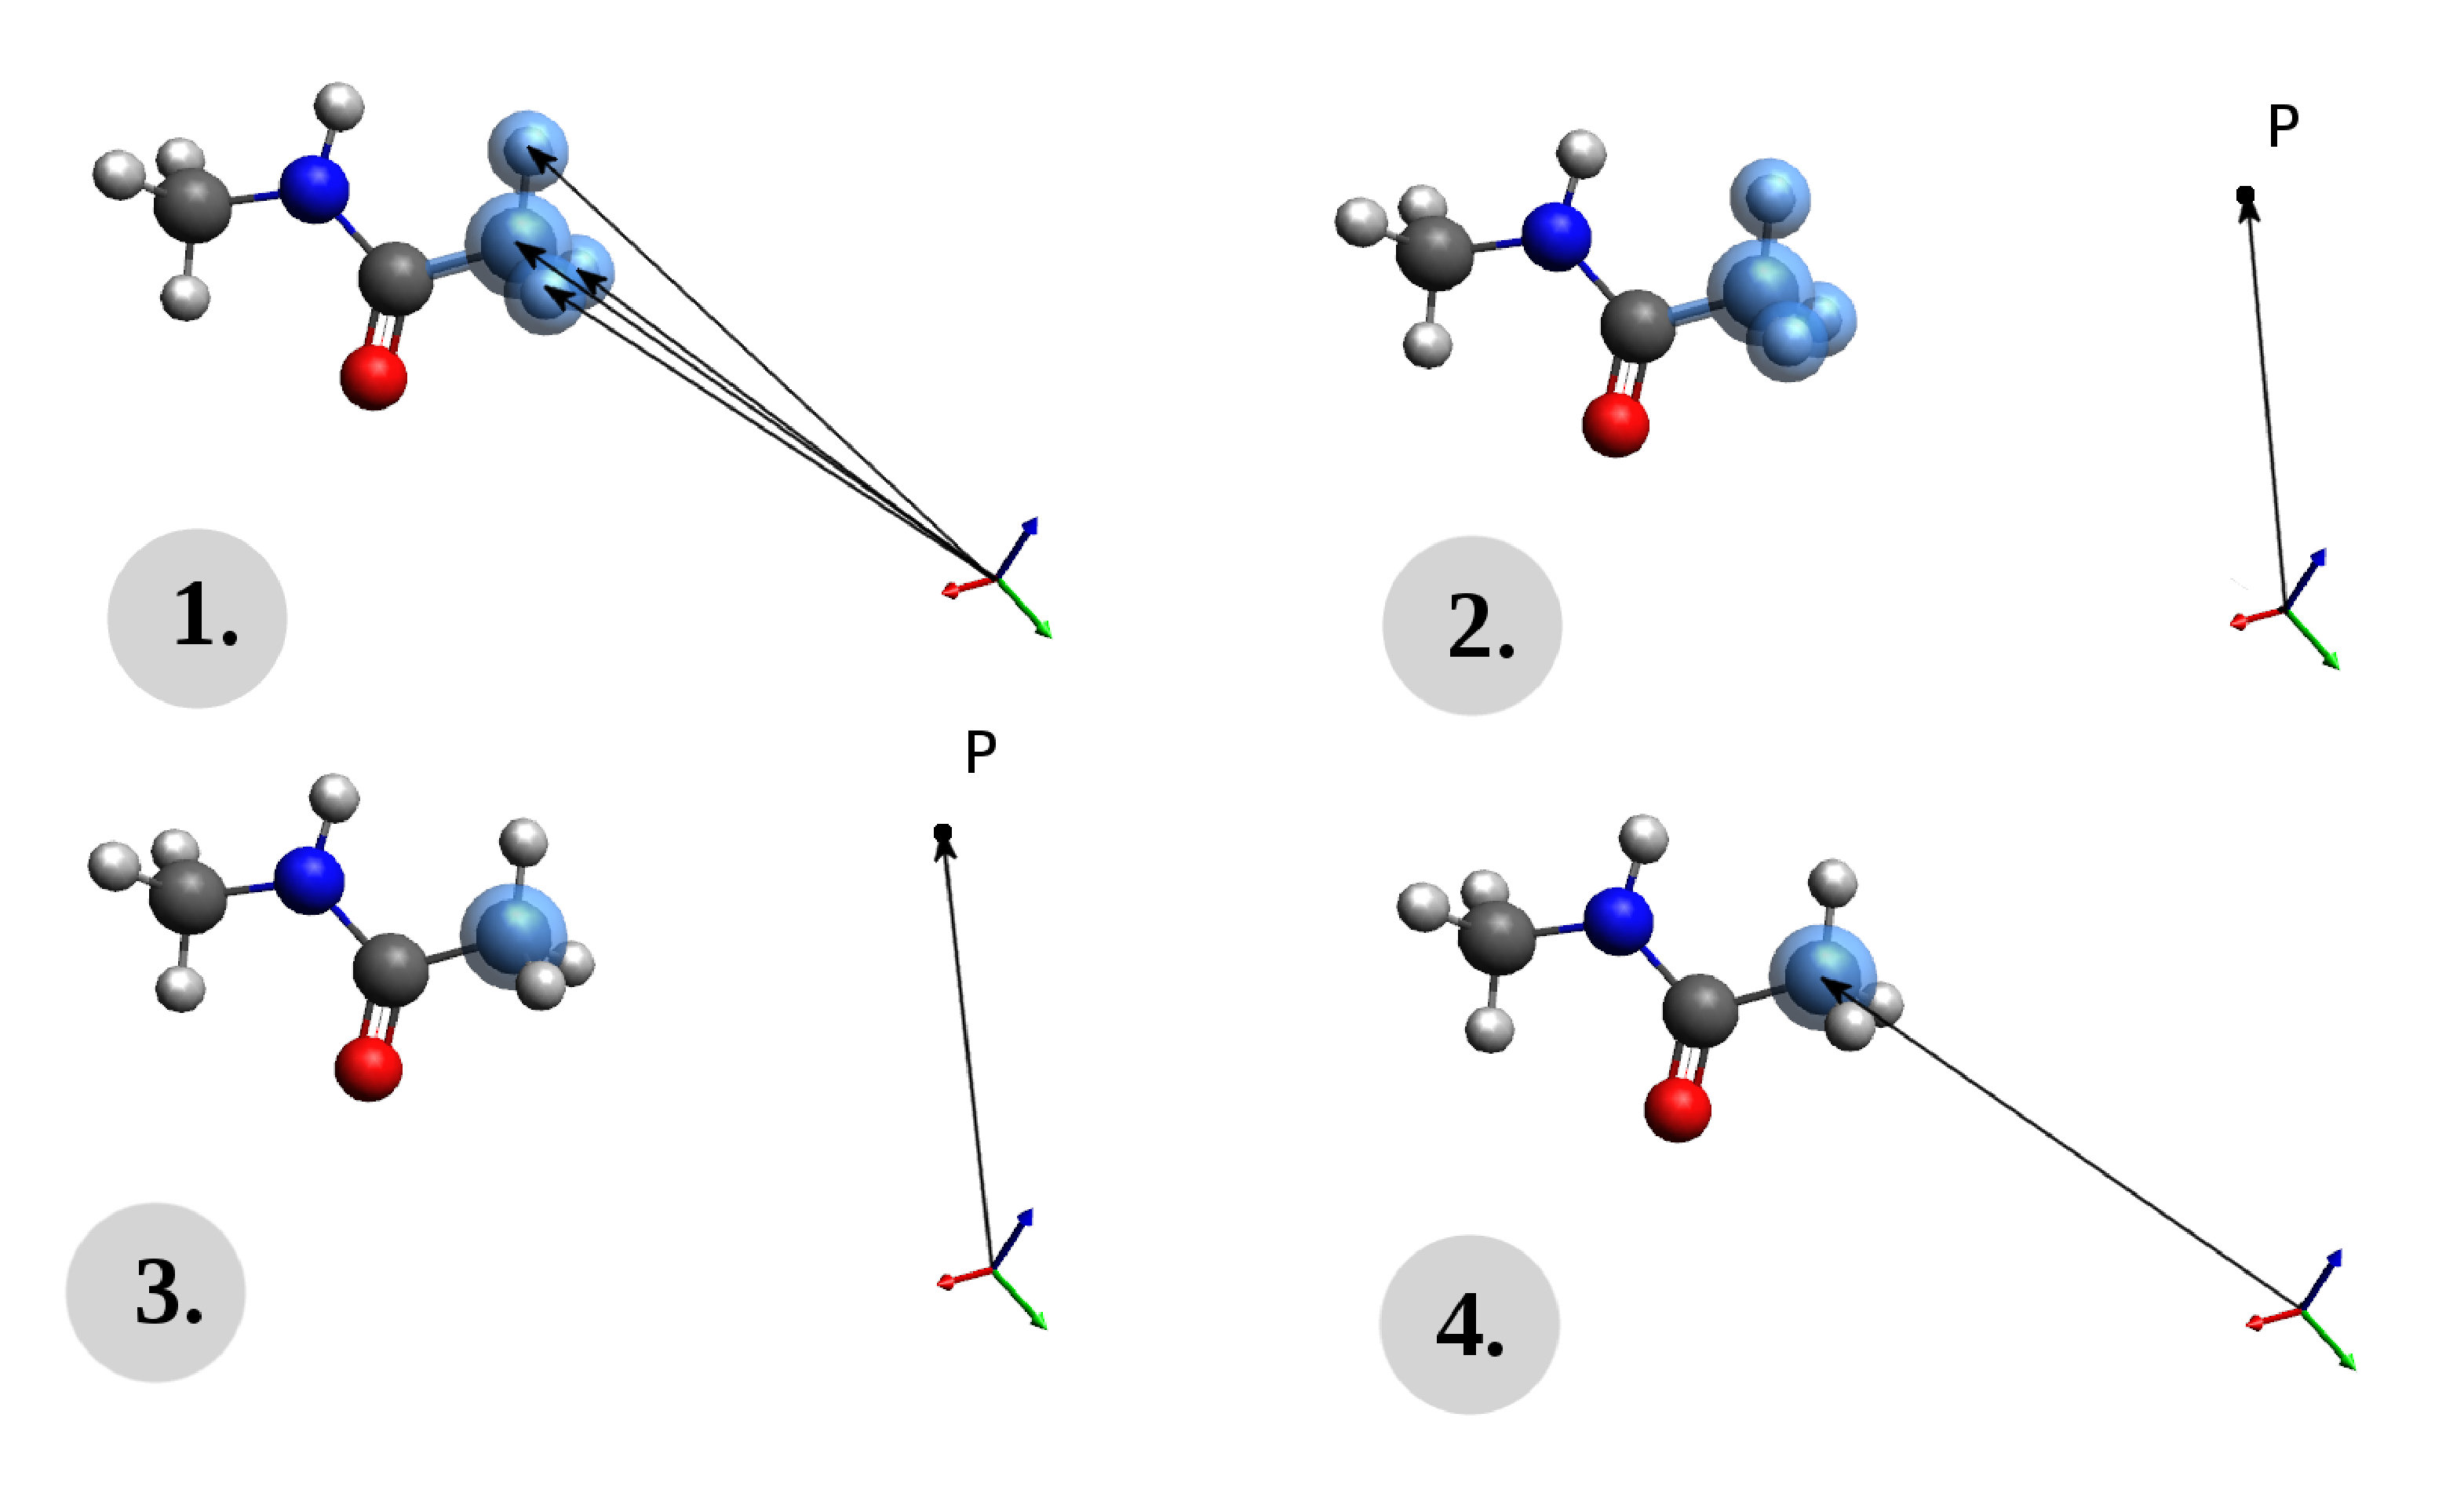
\includegraphics[width=0.9\linewidth]{contr.eps}
}
\caption{Construction of contracted SolCAMM-$n$ models. Here, as an example, we present
the construction of versions of SolCAMM-$12$ (or SolDMA-$12$) model for NMA. 
The example is shown for one of methyl groups which we approximate by a united atom 
placed on the corresponding carbon atom. The origins are depicted by arrows
whereas the multipole centres as blue spheres. 1) all the distributed multipoles 
are placed on each atom. Since they have different origins the cannot be summed up 
to obtain united atom. 2) Thus, it is necessary to shift their origins to one, 
arbitrary point P. From now on, all the multipoles have the same origin at P 
and they are additive. 3) All the multipoles for methyl group (four sets 
of multipoles for each atom) are summed over. The resulting united atom 
multipole moment has its origin at point P. 4) The centre of these multipoles 
is moved to the carbon atom position.
\label{f:contr}}
\end{figure}
%

%\begin{wrapfigure}{r}{0.30\textwidth}
%\vspace{-30pt}
\begin{figure}[b!]
\begin{center}
    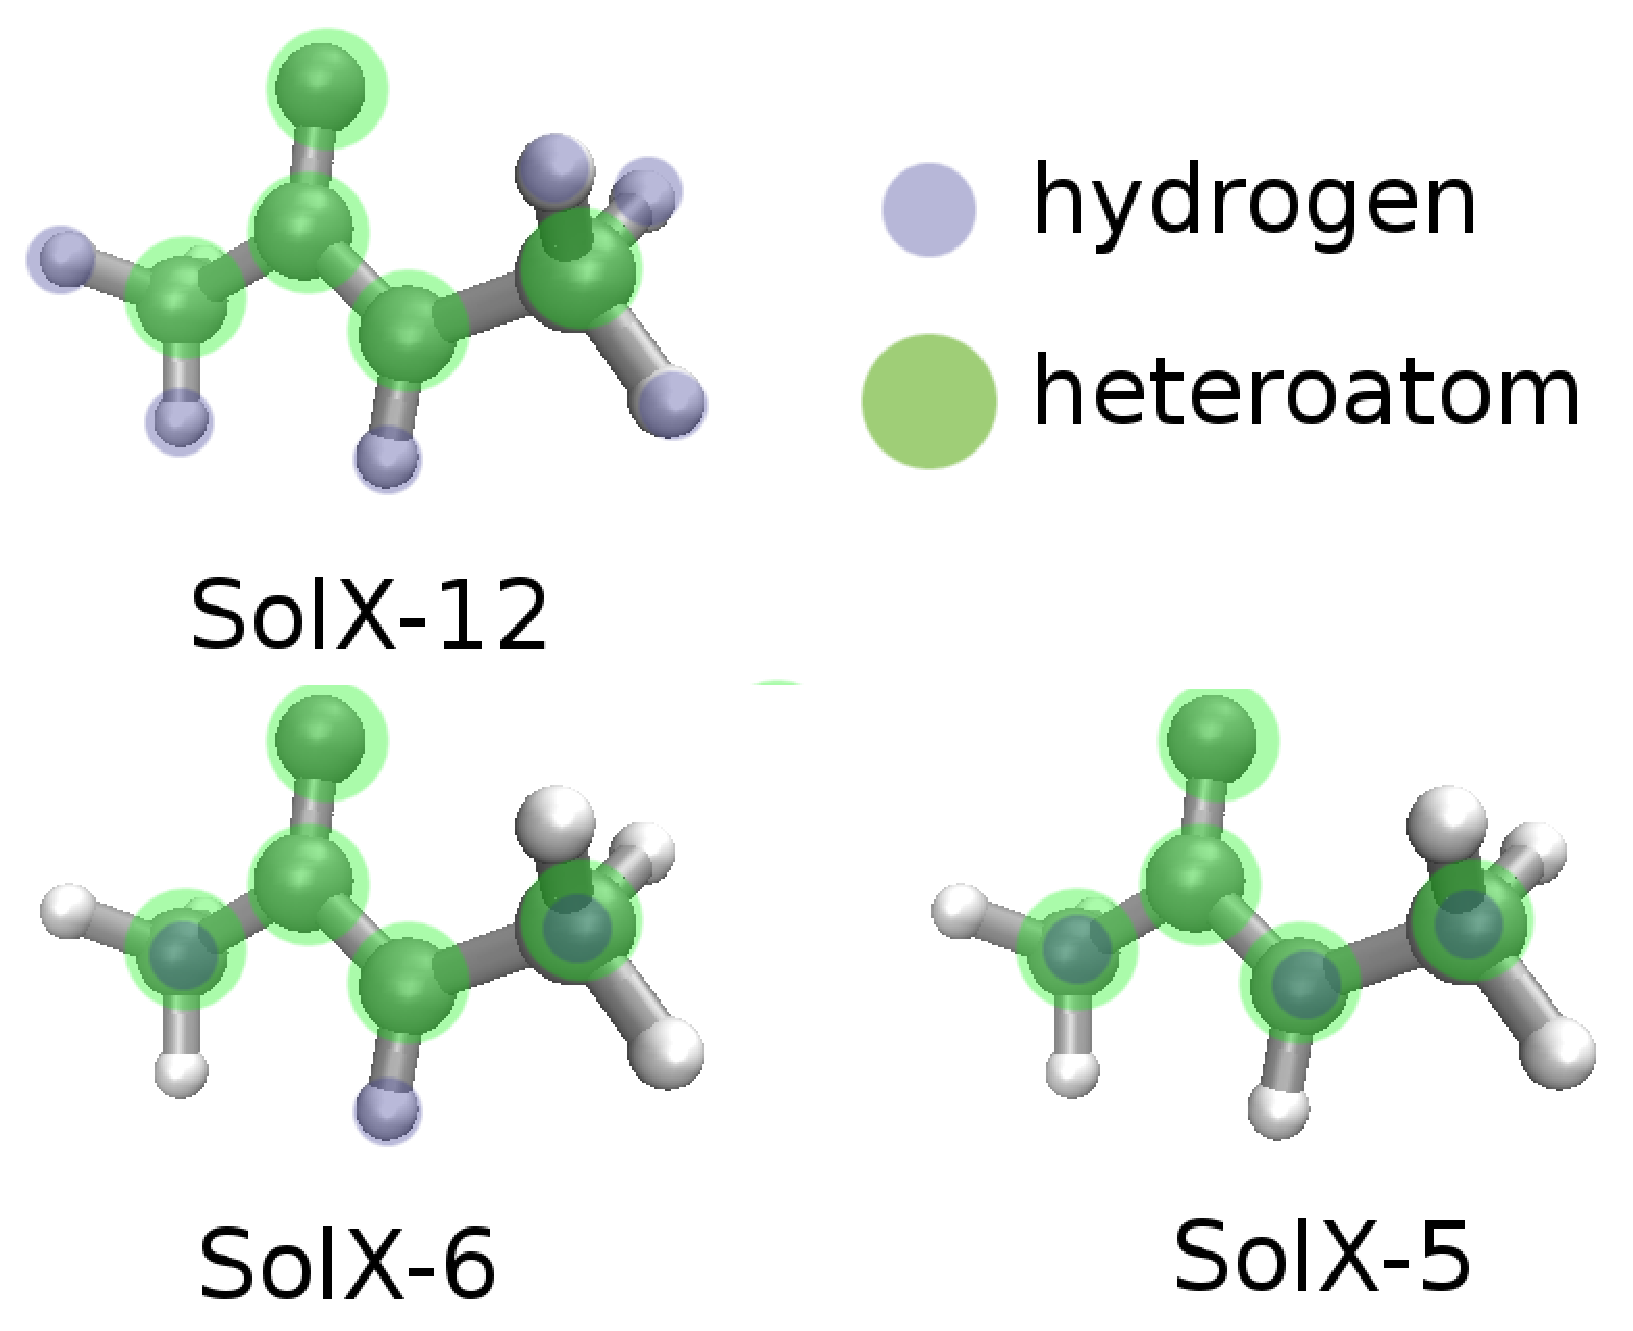
\includegraphics[width=0.28\textwidth]{SolXn.eps}
  \end{center}
%  \vspace{-18pt}
  \caption{Variants of SolX models for $N$-methyl acetamide amide I mode.
X denotes distributed atomic multipoles in this case (e.g., DMA or CAMM).\label{f:solxn}}
%\vspace{-20pt}
%\end{wrapfigure}
\end{figure}
%
\noindent This procedure can lead to the increase in the performance
of the method because the number of distributed centres
is decreased. If the contraction involves atoms that 
are not affected by the vibrational mode of interest (e.g. 
hydrogen atoms in the methyl group when one is interested
in amide I mode) the contracted models give basically 
the same results as uncontracted models. However, one needs to 
be aware that the united atom model obtained by this procedure
does not include the rotational averaging which might be of
interest when methyl groups are freely rotatable. These aspects 
will be discussed in more detail in the next Chapter. 

\subsection{SolEFP, SolEDS and SolSAPT Models\label{s:solefp-soleds-solsapt}}

To include also non\hyp{}Coulombic effects to describe 
the intermolecular interaction potential one can use, for example,
the following methods:
%
\begin{enumerate}
  \item Effective Fragment 
Potentials \citep{Day.Jensen.Gordon.Webb.Stevens.Krauss.Garmer.Basch.Cohen.JCP.1996,
Flick.Kosenkov.Hohenstein.Sherrill.Slipchenko.JCTC.2012} (EFP)
  \item Variational\hyp{}perturbational Interaction Energy Decomposition
Scheme \citep{Sokalski.Roszak.Pecul.CPL.1988,
Chalasinski.Szczesniak.MolPhys.1988,Cybulski.Chalasinski.Moszynski.JCP.1990,
Gora.Bartkowiak.Roszak.Leszczynski.JCP.2004} (EDS)
  \item Symmetry Adapted Perturbation Theory \citep{Jeziorski.Moszynski.Szalewicz.ChemRev.1994} (SAPT)
\end{enumerate}
%
These will lead to the SolEFP, SolEDS and SolSAPT methods, accordingly. 

\subsubsection{SolEFP Model\label{s:solefp-working-model}}

In fact, the SolEFP method was already described in Section~\ref{s:vibr-solv-explicit-models}
and the frequency shift is given as
%
\begin{equation} \label{e:dw-solefp}
\Delta\omega^{\rm SolEFP} = 
\Delta\omega^{\rm Coul} + \Delta\omega^{\rm Ind} + \Delta\omega^{\rm Disp}_6 +
\Delta\omega^{\rm Ex-Rep} + \Delta\omega^{\rm CT}
\end{equation}
%
with $\Delta\omega^{\rm Coul}$ given by Eq.~\eqref{e:dw-solefp-coul-working},  
$\Delta\omega^{\rm Ind}$ by Eq.~\eqref{e:dw-ind-avec},
$\Delta\omega^{\rm Disp}_6$ by Eq.~\eqref{e:dw-disp-6-distr-working},
$\Delta\omega^{\rm Ex-Rep}$ by Eq.~\eqref{e:dw-exrep-base},
and $\Delta\omega^{\rm CT}$ by Eq.~\eqref{e:dw-ct}.
Thus, SolCAMM (or SolDMA) is a part of SolEFP method.
The above expression can be recast in the following form
%
\begin{equation} \label{e:dw-solefp-electric-nonelectric}
\Delta\omega^{\rm SolEFP} = 
\Delta\omega^{\rm Electric} + \Delta\omega^{\rm Non-Electric}
\end{equation}
%
where
%
\begin{subequations} 
\begin{align}
\Delta\omega^{\rm Electric}       &=  \Delta\omega^{\rm Coul} + \Delta\omega^{\rm Ind} \label{e:dw-solefp-electric} \\ 
 \Delta\omega^{\rm Non-Electric}  &=  \Delta\omega^{\rm Disp}_6 +
\Delta\omega^{\rm Ex-Rep} + \Delta\omega^{\rm CT} \label{e:dw-solefp-nonelectric}
\end{align}
\end{subequations}
%
The components which cannot be described by no means by interactions
with electric fields  will be analysed later in Chapter~\ref{c:cn-modes}.

It is also straightforward to compute the 
solvation\hyp{}induced transition dipole change
with SolEFP vibrational forces according to the following prescription
%
\begin{multline} \label{e:dmu-solefp}
\Delta\left(\frac{{\BM \upmu}}{Q_j}\right) \equiv 
 \frac{\partial{\BM \upmu}({\bf F},U)}{\partial\overline {\bf Q}_j} \Bigg|_{\overline{\bf Q}_{0_A}} -  
 \frac{\partial{\BM \upmu}({\bf F}={\bf 0},U=0)}{\partial {\bf Q}_j} \Bigg|_{{\bf Q}_{0_A}} \approx
%
\sum_a 
\fderiv{{\BM \alpha}_{a}}{Q_j} \cdot {\bf F}({\bf r}_a) \\
+
\sum_i 
\frac{1}{M_i\omega_i^2} 
\left[
 U^{\rm Coul}_i   + 
 U^{\rm Ind}_i    +
 U^{\rm Disp}_{6;i}   +
 U^{\rm Ex-Rep}_i +
 U^{\rm CT}_i
\right]
%
\left\{ 
 \sderivd{{\BM \upmu}_0}{Q_j}{Q_i} 
 + \sum_a \sderivd{{\BM \alpha}_{a}}{Q_j}{Q_i} \cdot {\bf F}({\bf r}_a)
%
\right\}  
\end{multline}
%
where the vibrational forces along the $i$th normal coordinate
$U_i$ due to Coulombic, induction, dispersion, exchange\hyp{}repulsion
and charge transfer effects are given in Eqs.~\eqref{e:f-terms},
\eqref{e:vibr-force-ind}, \eqref{e:vibr-force-disp-6}, 
\eqref{e:force-exrep} and \eqref{e:force-ct-ab}, respectively.
Note that these terms correspond to the interaction\hyp{}induced
molecular structure relaxation effect
whereas the first term in Eq.~\eqref{e:dmu-solefp}
refers to the induction effect originating purely from
electronic relaxation (i.e., without structural distortion).

%\paragraph{Features and limitations of SolEFP approach}
Due to its intrinsic fragmentation framework \citep{Gordon.Fedorov.Pruitt.Slipchenko.ChemRev.2012}, 
SolEFP is suitable for modelling very large systems
ranging from bulk solutions to highly heterogeneous
protein environments \citep{Blasiak.Ritchie.Webb.Cho.PCCP.2016} 
(see Chapter~\ref{c:cn-modes}). Note that in order
to compute the solvation\hyp{}induced frequency shift or the
transition dipole moment change, one needs the information
about the gas\hyp{}phase states of the molecules \emph{only}, 
because the effects of their interactions do not require 
any other specific solute\hyp{}solvent information.
This is a great advantage over SolEDS and SolSAPT approaches
which are limited to studying only small multimers because 
they require calculations of the wavefunctions for the whole
solute\hyp{}solvent complex. On the other hand, the price
which we need to pay for coarse\hyp{}grained character of the SolEFP model
is accuracy.
%according to 
%previous sections, SolEFP espression in Eq.~\eqref{e:dw-solefp} 
%is an approximation of the local mode approximation from
Eq.~\eqref{e:buckingham-2st-order-total-fund}. 
Let us 
explicitly list all the approximations upon which SolEFP presented in 
this Thesis is based:
%
\begin{itemize}
 %
 \item The charge\hyp{}penetration effects have been ignored, since they are likely to be weak. 
Nevertheless, since they were found to be of importance in accurately describing 
the Coulomb interaction energy of many systems \citep{Slipchenko.Gordon.JCC.2007}, 
such charge\hyp{}penetration 
effects on the vibrational solvatochromism need to be studied in the future. Fortunately,
the current distributed multipole approximation works well for vibrational frequency shifts
when compared with exact results. \citep{Blasiak.Cho.JCP.2014,Blasiak.Cho.JCP.2015,
Blasiak.Ritchie.Webb.Cho.PCCP.2016,Maj.Ahn.Blasiak.Kwak.Han.Cho.XXX.2016}
 %
 \item Due to the complexity of the SolEFP equations, we did not take into account the electric 
anharmonicity contributions, except for that associated with the Coulomb interaction\hyp{}induced 
frequency shift. When the exchange\hyp{}repulsion, induction, and dispersion terms in the frequency 
shift calculation are estimated, only the first derivatives of potential energy with respect 
to normal coordinates are considered. We already showed that this approximation is quite acceptable 
for describing the carbonyl and CN stretch modes. \citep{Blasiak.Cho.JCP.2014,Blasiak.Cho.JCP.2015,
Blasiak.Ritchie.Webb.Cho.PCCP.2016}
However, for completeness it will be necessary to further test the validity of this approximation 
for other IR probes. In particular, we noticed that in the case of amide II mode
electronic anharmonicity of exchange\hyp{}repulsion contribution cannot be ignored. \citep{Blasiak.Cho.JCP.2015}
 %
 \item The exchange\hyp{}repulsion interaction\hyp{}induced frequency shift was based on the approximation 
that only a single exchange of electron pair between solute and solvent is considered. 
Fortunately, it was shown that higher\hyp{}order electron pair exchanges contribute
negligibly to the Heitler\hyp{}London energies. \citep{Korona.Williams.Bukowski.Jeziorski.Szalewicz.JCP.1997}
In fact, it is believed here that this is an excellent approximation also for vibrational
solvatochromic frequency shifts because the direct comparisons 
of the SolEFP results with completely \emph{ab initio}\footnote{SolEDS} calculation results indicate 
that the current SolEFP exchange\hyp{}repulsion frequency shifts are quite accurate (see
Chapter~\ref{s:solefp-soleds-solsapt}). %chapter about SolEDS calculations, probably the next chapter
 %
 \item Induction and dispersion interaction\hyp{}induced frequency shifts 
were treated by taking into consideration only the dipole\hyp{}dipole interactions 
between LMO polarizable centres. Perhaps, the dispersion interaction\hyp{}induced 
contribution originating from distributed quadrupole\hyp{}dipole and quadrupole\hyp{}quadrupole 
interactions could be of importance as well.
 %
 \item Exchange effects are taken into account only for the short\hyp{}range
interactions such as first\hyp{}order exchange\hyp{}repulsion and charge\hyp{}transfer, whereas 
they are ignored for induction and dispersion effects. On the other hand,
the exchange\hyp{}dispersion interaction energy was found to be very small
for H-bonded complexes. \citep{Langlet.Caillet.Caffarel.JCP.1995,
Zierkiewicz.Jurecka.Hobza.ChemPhysChem.2005,Cybulski.Sadlej.JCTC.2008} 
Also, induction vibrational frequency shifts
under mechanical anharmonicity approximation
are very well reproduced within SolEFP model as compared to benchmark 
calculations. \citep{Blasiak.Cho.JCP.2014,Blasiak.Cho.JCP.2015,
Blasiak.Ritchie.Webb.Cho.PCCP.2016,Maj.Ahn.Blasiak.Kwak.Han.Cho.XXX.2016}
 %
 \item Due to
large computational demands, CT contributions are not computed at present implementation
of SolEFP. We have tested Eq.~\eqref{e:dw-ct} for NMA--water dimers 
with approximating the potential integrals and their derivatives by invoking the distributed
charge approximation (Eq.~\eqref{e:ct-v-qy}) with ChelpG method. \citep{Breneman.Wiberg.JCC.1990} 
Fortunately,
it turned out that CT effects are negligible for the vibrational solvatochromic frequency shifts
(we obtained contributions of the order 2~cm$^{-1}$ and smaller in that case). In addition, it was shown
that CT effects are not of concern 
for many important IR probes interacting with water. \citep{Lee.Choi.Cho.PCCP.2010,Blasiak.Cho.JCP.2014}
 %
 \item Since the SolEFP theory is to calculate all the vibrational solvatochromism parameters 
that can be obtained from \emph{ab initio} calculations of the solute molecule in the gas phase, 
the same structure should be used when the theory is applied to the solution systems 
with a solute molecule surrounded by solvent molecules. Therefore, there exists a certain 
ambiguity (difficulty) in perfectly superimposing it onto the solute molecule in solutions 
-- note that the detailed molecular structures (bond lengths, bond angles, and so on) 
of solute molecules in solutions are slightly different from that in the gas phase 
due to electronic structure change induced by solute\hyp{}solvent intermolecular interactions. 
Nevertheless, it should be emphasised that the present vibrational solvatochromism theory 
correctly includes the effects from solvation\hyp{}induced structural distortions 
since they are related to mechanical anharmonicity in the corresponding potential 
energy surface. Therefore, the above difficulty may not be the most crucial one, 
but still it needs to be investigated more in detail. We will refer to this issue as to
the \emph{superimposition problem}.
 %
\end{itemize}
%
It was reported that EFP2 interaction energies were shown to be
in reasonable agreement 
with SAPT. \citep{Flick.Kosenkov.Hohenstein.Sherrill.Slipchenko.JCTC.2012} 
Nevertheless, before SolEFP method is used, first it has to be validated
against more accurate approach -- SolEDS or SolSAPT. 

\subsubsection{SolEDS Model\label{s:soleds}}

One of easy ways of computing the total interaction energy
between two molecules is to adopt the supramolecular approach
in which the interaction energy is defined as
%
\begin{equation} \label{e:e-int-supramol}
 U = E_{AB} - E_A - E_B
\end{equation}
%
In the above expression, the internal coordinates of molecules $A$ and $B$
are the same with those of the dimer $AB$.
According to the EDS scheme \citep{Sokalski.Roszak.Pecul.CPL.1988,
Chalasinski.Szczesniak.MolPhys.1988,Cybulski.Chalasinski.Moszynski.JCP.1990,
Gora.Bartkowiak.Roszak.Leszczynski.JCP.2004}, the HF
intermolecular interaction energy in the supramolecular
approach from Eq.~\eqref{e:e-int-supramol} can be decomposed
into the following terms
%
\begin{equation}
 U^{\rm HF} = \Delta E_{\rm el}^{(10)}    + 
              \Delta E_{\rm ex}^{\rm HL}  +
              \Delta E_{\rm del}^{\rm HF}
\end{equation}
%
where $\Delta E_{\rm el}^{(10)}$ represents the first\hyp{}order 
Coulombic interaction
between unperturbed solute and solvent charge densities, 
$\Delta E_{\rm ex}^{\rm HL}$ is the corresponding exchange\hyp{}repulsion
correction to properly take into account the antisymmetry of the wavefunction,
$\Delta E_{\rm del}^{\rm HF}$ is the remainder describing charge delocalization
effects (induction, charge transfer and mixing terms). The first two terms
are the Heitler\hyp{}London energy
%
\begin{equation}
 \Delta E^{\rm HL} = \Delta E_{\rm el}^{(10)}    + 
                     \Delta E_{\rm ex}^{\rm HL}
  = \frac{
\langle \mathscr{A} 0_A0_B \lvert \mathscr{V}_{AB} \rvert \mathscr{A} 0_A0_B \rangle 
}{
\langle \mathscr{A} 0_A0_B \vert \mathscr{A} 0_A0_B \rangle 
}
\end{equation}
%
The Coulombic contribution can be technically split into the following
two
%
\begin{equation}
 \Delta E_{\rm el}^{(10)} = \Delta E_{\rm el}^{\rm DMTP} + \Delta E_{\rm el}^{\rm PEN}
\end{equation}
%
where $\Delta E_{\rm el}^{\rm DMTP}$ is obtained from the distributed multipole 
analysis (DMTP) result\footnote{CAMM, DMA or LMTP} whereas
$\Delta E_{\rm el}^{\rm PEN}$ accounts for the short\hyp{}range charge\hyp{}penetration
effects. It is important to remember that the latter is purely quantum mechanical in
nature and cannot be treated by any multipole expansion approach which also diverges
quickly for small intermolecular separations.
Charge penetration can be, however, included by using \emph{ad hoc} damping factors
that appropriately scale the interactions between distributed multipole
moments according to their relative distance. \citep{Slipchenko.Gordon.JCC.2007,Wang.Truhlar.JCTC.2010}
Also, Stone recently derived fully \emph{ab initio} formulae
for the damping factors based on the Gaussian multipoles. \citep{Stone.JPCA.2011}
The potential future
first\hyp{}principles solvatochromic
models including $\Delta E_{\rm el}^{\rm PEN}$ should follow his study.

So far, we have focused on the HF wavefunctions only. \citep{Roothaan.RevModPhys.1951} 
However, including
electron correlation energies below the Fermi level is generally important
for chemistry. One of the simplest approaches to include the 
so called dynamic electron correlation\footnote{associated with
the interactions of the occupied and virtual molecular orbitals}
is to assume the 
M{\o}ller\hyp{}Plesset approximation \citep{Moller.Plesset.PhysRev.1934}
in which some specific forms of the doubly\hyp{}excited Slater
determinants contribute to the ground state wavefunction.
According to EDS technique, MP2 interaction energy is
partitioned into
%
\begin{equation}
 U^{\rm MP2} = U^{\rm HF}                    + 
               \Delta E_{\rm el,r}^{(12)}    + 
               \Delta E_{\rm ex}^{(2)}       +
               \Delta E_{\rm disp}^{(20)}  
\end{equation}
%
where $\Delta E_{\rm el,r}^{(12)}$ and $\Delta E_{\rm ex}^{(2)}$
are the electron correlation corrections to the first\hyp{}order
electrostatic interaction and the remaining effects at HF level,
respectively. The second\hyp{}order dispersion energy
is denoted by $\Delta E_{\rm disp}^{(20)}$. In EDS calculations
of both HF or MP2 levels,
all the interaction energy components are evaluated in DCBS.

Now, we define the SolEDS method as
%
\begin{equation} \label{e:dw-soleds}
 \Delta\omega_j^{\rm SolEDS} = \left(\hat{F}_j^{\rm EA} + \hat{F}_j^{\rm MA}\right)  U^{\rm HF\text{ or }MP2} 
\end{equation}
%
which leads to the following contributions to the vibrational
frequency shift
%
\begin{equation} \label{e:dw-soleds-hf}
 \Delta\omega_j^{\rm SolEDS//HF} = 
              \Delta \omega_{j;{\rm el}}^{(10)}    + 
              \Delta \omega_{j;{\rm ex}}^{\rm HL}  +
              \Delta \omega_{j;{\rm del}}^{\rm HF}
\end{equation}
%
and
%
\begin{equation} \label{e:dw-soleds-mp2}
 \Delta\omega_j^{\rm SolEDS//MP2} = 
              \Delta \omega_{j;{\rm el}}^{(10)}    + 
              \Delta \omega_{j;{\rm ex}}^{\rm HL}  +
              \Delta \omega_{j;{\rm del}}^{\rm HF} +
               \Delta \omega_{j;{\rm el,r}}^{(12)}    + 
               \Delta \omega_{j;{\rm ex}}^{(2)}       +
               \Delta \omega_{j;{\rm disp}}^{(20)}  
\end{equation}
%
The operators $\hat{F}_j^{\rm EA}$ and $\hat{F}_j^{\rm MA}$
are defined in Eqs.~\eqref{e:dw-fea} and \eqref{e:dw-fma}, respectively.
It is important to emphasise here that the vibrational analysis 
calculations performed at the HF and MP2 levels are based on different
vibrational potential energy surfaces so that the $\Delta \omega_{j;{\rm el}}^{(10)}$,
$\Delta \omega_{j;{\rm ex}}^{\rm HL}$ and $\Delta \omega_{j;{\rm del}}^{\rm HF}$ 
part of $\Delta\omega_j^{\rm SolEDS//MP2}$ quantitatively differs from
$\Delta\omega_j^{\rm SolEDS/HF}$ obtained at the HF level of theory,
though the same notation is used in both Eqs.~\eqref{e:dw-soleds-hf} 
and \eqref{e:dw-soleds-mp2}.

\subsubsection{SolSAPT Model\label{s:solsapt}}

If one wants to go beyond HF and MP2 levels and
analyse the origins of the vibrational frequency 
shifts at, for instance, coupled cluster
level, one should use SAPT decomposition of the interaction
energy which is
the most rigorous and accurate method up to date for that purpose.
In the simplest correlated SAPT scheme, the energy operator
is partitioned as follows
%
\begin{equation}
 \mathscr{H}^{AB} = \mathscr{F}^{A} + \mathscr{F}^{B} + \lambda \mathscr{W}^{AB} + \varsigma \mathscr{U}^{AB}
\end{equation}
%
where $\mathscr{F}^{A}$ is the Fock operator of isolated molecule $A$, 
$\mathscr{W}^{AB}$ is the electron correlation operator 
whereas $\mathscr{U}^{AB}$ is the interaction\hyp{}energy operator.
Parameters $\lambda$ and $\varsigma$ refer to the two perturbations
to the zeroth\hyp{}order operator $\mathscr{F}^{A}+\mathscr{F}^{B}$
and define the orders of a double exchange\hyp{}perturbation theory
for the interaction energies as
%
\begin{equation}
  E^{(nm)} =  E^{(nm)}_{\rm pol} +  E^{(nm)}_{\rm ex}
\end{equation}
%
where the superscripts $n$ and $m$ refer to the order in the
intermolecular interaction and electron correlation correction,
respectively. Each $nm$th order term can be split into the long\hyp{}range
polarization term $E^{(nm)}_{\rm pol}$ ($\mathscr{A}=\mathbb{1}$)
and the associated exchange\hyp{}repulsion correction $E^{(nm)}_{\rm ex}$,
where usually single electron exchange is assumed.
Thus, the solute\hyp{}solvent interaction potential can be written as
%
\begin{multline}
U^{\rm SAPT} =
         E^{(10)}_{\rm Coul} + E^{(10)}_{\rm Ex} + 
         E^{(20)}_{\rm Ind}  + E^{(20)}_{\rm Ex-Ind} +
         E^{(20)}_{\rm Disp} + E^{(20)}_{\rm Ex-Disp} \\ +
     \sum_m \left\{ E^{(1m)}_{\rm Coul} + E^{(1m)}_{\rm Ex-Rep} + E^{(2m)}_{\rm Disp}\right\} 
     + \ldots
\end{multline}
%
Note that electron correlation manifests
already in zeroth order in $m$ for $n=2$, which is the purely intermolecular
dispersion energy. $E^{(1m)}_{\rm Coul}$ and $E^{(1m)}_{\rm Ex-Rep}$
contain also intra\hyp{}molecular electron correlation corrections.
In the Table~\ref{t:sapt-eds-efp2} we depict the approximate relationships
between a few SAPT terms with EDS and EFP2 terms.
%
\begin{table}[ht]
\caption{Approximate correspondence between a few SAPT interaction
energy terms with EDS partitioning and EFP2 interaction potential
contributions.
\label{t:sapt-eds-efp2}}
\begin{tabular*}{1.0\textwidth}{@{\extracolsep{\fill} } l l l l}
\hline\hline
%\multicolumn{5}{c}{Amide I mode} \\
SAPT                     & EDS                             & EFP2               \\
\hline
%\multirow{5}{*}{A}   & SolCAMM   & -39.4 (+6.2)  & 5.3 (+0.9) & -34.1 (+7.1) \\
$E^{(10)}_{\rm Coul}$    & $\Delta E_{\rm el}^{(10)}$      &  $U^{\rm Coul}$    \\
$E^{(10)}_{\rm Ex}$      & $\Delta E_{\rm ex}^{\rm HL}$    &  $U^{\rm Ex-Rep}$  \\
$E^{(20)}_{\rm Ind}$     & $\sim\Delta E_{\rm del}^{\rm HF}$ &$U^{\rm Ind}$     \\
$E^{(20)}_{\rm Disp}$    & $\Delta E_{\rm disp}^{(20)}$    &  $U^{\rm Disp}$    \\
$E^{(12)}_{\rm Coul}$    & $\Delta E_{\rm el,r}^{(12)}$    &  --                \\
$E^{(12)}_{\rm Ex}+E^{(20)}_{\rm Ex}$    & $\sim \Delta E_{\rm ex}^{(2)}$ &  -- \\
$\left(E^{(20)}_{\rm Ind} + E^{(20)}_{\rm Ex-Ind}\right)$[DCBS] $-$
   & \multirow{2}{*}{Included in $\Delta E_{\rm del}^{\rm HF}$  } & \multirow{2}{*}{$U^{\rm CT}$} \\
$\left(E^{(20)}_{\rm Ind} + E^{(20)}_{\rm Ex-Ind}\right)$[MCBS] &       & & \\
\hline\hline
\end{tabular*}
\end{table}
%
Analogously,
the SolSAPT vibrational frequency shift is defined as
%
\begin{equation}
 \Delta\omega_j^{\rm SolSAPT} = \left(\hat{F}_j^{\rm EA} + \hat{F}_j^{\rm MA}\right) U^{\rm SAPT} 
\end{equation}
%
where we have 
%
\begin{multline} \label{e:dw-solsapt}
 \Delta\omega_j^{\rm SolSAPT} =
        \Delta\omega^{(10)}_{j;{\rm Coul}} + \Delta\omega^{(10)}_{j;{\rm Ex}} + 
        \Delta\omega^{(20)}_{j;{\rm Ind}}  + \Delta\omega^{(20)}_{j;{\rm Ex-Ind}} +
        \Delta\omega^{(20)}_{j;{\rm Disp}} + \Delta\omega^{(20)}_{j;{\rm Ex-Disp}} \\ +
     \sum_m \left\{\Delta\omega^{(1m)}_{j;{\rm Coul}} +
                   \Delta\omega^{(1m)}_{j;{\rm Ex-Rep}} + 
                   \Delta\omega^{(2m)}_{j;{\rm Disp}}\right\} + \ldots
\end{multline}
%
In the above equation, the appropriate contributions can be
more or less identified with SolEDS and SolEFP frequency shifts
according to Table~\ref{t:sapt-eds-efp2}.

\section{Going Beyond Weak Coupling Approximation\label{s:beyond-wca}}

Weak coupling approximation, i.e., Eq.~\eqref{e:buckingham-2st-order-total-fund},
was shown to be an excellent approximation
for vibrational modes that are fairly local in character
such as C$-$H, C$-$F, C$-$Cl, C$-$Br, C$\equiv$N and C$=$O stretches. However, it
is not in general valid for an arbitrary normal mode
which is sensitive to coupling with other types of motion
in the molecule when $U$ perturbs the Hamiltonian.
In fact, the more atomic overlap two harmonic modes have,
the easier for them is to mix with each other
upon solvation to lower the energy
of the system. 
%As for now, it is unclear whether azides modes
%an be described by LMA or not, since no first\hyp{}principles
%evaluation of this approximation for azides was undertaken.
%It is well known that azide stretch mode has two frequencies,
%which is antisymmetric and symmetric stretch. They both
%are delocalized over 3 atoms. This situation is far more different
%from SCN group in which CN vibration is fairly isolated
%from much heavier and chemically different S atom.
Therefore, it is necessary to extend WCA approximation
within the framework of SolEFP (and SolEDS) models
to take into account the intramolecular mode mixing
phenomenon. As an example case, we will point this out
in Chapter~\ref{c:mode-mixing-guanines} 
where we analyse ring deformation modes
of guanine. They are delocalized over at least 4 atoms
and exhibit substantial mixing between themselves.

\subsection{Towards Quantitative Modelling}

The foundations of the necessary theory were developed
by Cho. \citep{Cho.JCP.2009} Although he focused on the coarse\hyp{}grained
vibrational electrochromism due to a set of surrounding
multipoles, he derived the general form of the solute's
Hessian matrix when $U$ is added to the vibrational potential
energy function:
%
\begin{equation} 
 \tilde{k}_{jk} = \omega_j^2 \delta_{jk} + \frac{1}{\sqrt{M_jM_k}}\sderivd{U}{Q_j}{Q_k}  \Bigg|_{{\bf Q}_{0_A}} 
                           - \frac{1}{\sqrt{M_jM_k}}\sum_i g_{ijk} 
                             \frac{1}{M_i\omega_i^2}\fderiv{U}{Q_i}          \Bigg|_{{\bf Q}_{0_A}}        
\end{equation}
%
which, within the SolEFP framework, can be recast in
the form from Eq.~\eqref{e:jeden} with $\tilde{\bf U}$
defined by
%
\begin{equation} \label{e:dwa}
 \tilde{\bf U} = \sum_{\rm Int} \tilde{\bf U}^{\rm Int}
\end{equation}
%
with
%
\begin{equation}  \label{e:trzy}
 \tilde{U}^{\rm Int}_{jk} = \frac{1}{\sqrt{M_jM_k}} \left\{
            \sderivd{U^{\rm Int}}{Q_j}{Q_k}  \Bigg|_{{\bf Q}_{0_A}} 
           - \sum_i g_{ijk} \frac{1}{M_i\omega_i^2}\fderiv{U^{\rm Int}}{Q_i} \Bigg|_{{\bf Q}_{0_A}} 
           \right\}
\end{equation}
%
and $\rm Int$ denoting Coulombic, induction, dispersion, exchange\hyp{}repulsion
and CT effects. 
%Eqs.~\eqref{e:dwa} and \eqref{e:trzy}.
Ideally, one could just compute all
$\tilde{\bf U}^{\rm Int}$ matrices. However, in terms of
computational demands this is very costly due to the
need of computing all the second derivatives of $U$
with respect to all the normal coordinates of solute.
This gives $(3N-6)^2$ derivatives for each interaction
type. Moreover, the diagonalisation of the entire Hessian
matrix would probably cause problems because the quantitative
description of the structural distortions
along the coordinates associated with low frequency modes
is still not fully resolved issue (see Section~\ref{s:str-dist-general-discussion}). 
Fortunately, it is likely that the normal modes
are not coupled with each other equally strong. Therefore,
one could partition force constant matrix into \emph{blocks}
and focus only on the normal modes of interest. As a limiting
cases we shall study the two\hyp{} and three\hyp{}mode
couplings. 
%The first might be related to the azide symmetric
%and asymmetric stretches
%while
In particular, the three\hyp{}mode coupling model 
could be considered to study the mode mixing of
guanine ring modes that appear around 1550~cm$^{-1}$.

\subsection{Coupling Between Two Modes\label{s:coupling-between-2-modes}}

When our mode of interest $j$ is strongly coupled
with $k$th mode we need to diagonalise 2x2 Hessian matrix.
Thus, the two vibrational frequencies are given by
%
\begin{equation} \label{e:11aa11aa}
 \overline{\omega}^2 = %\sqrt{
\frac{ \tilde{k}_{jj} + \tilde{k}_{kk} }{2}
\pm \frac{1}{2}
\sqrt{\left( \tilde{k}_{jj} - \tilde{k}_{kk}\right)^2 - 4\tilde{k}_{jk}^2}
%}
\end{equation}
%
and the transformation matrix $\bf X$ becomes
%
\begin{equation} \label{e:ohoho}
 {\bf X} = 
\begin{bmatrix}
\cos{\theta} &   \sin{\theta}\\ 
\sin{\theta} &  -\cos{\theta}
\end{bmatrix}
\end{equation}
%
with
%
\begin{equation}
\theta = \frac{1}{2} \tan^{-1}\left\{\frac{2\tilde{k}_{jk}}{\tilde{k}_{jj} - \tilde{k}_{kk}}\right\} 
 \approx \frac{\tilde{k}_{jk}}{\tilde{k}_{jj} - \tilde{k}_{kk}} \qquad\text{for small $\tilde{k}_{jk}$}
\end{equation}
%
Let us analyse the relation in Eq.~\eqref{e:11aa11aa} more closely
since, in fact, in some cases not all terms will strongly contribute to the new vibrational
frequency. We can write that
%
\begin{multline}
 \left( \tilde{k}_{jj} - \tilde{k}_{kk}\right)^2 = 
 \left( \left[ \omega_j^2 - \omega_k^2 \right] 
 +
 2\left[ \omega_j\Delta\omega_j - \omega_k\Delta\omega_k \right]\right)^2 \\
 \approx \left( \omega_j^2 - \omega_k^2 \right)^2
 + 4 \left[ \omega_j\Delta\omega_j - \omega_k\Delta\omega_k \right] \left( \omega_j^2 - \omega_k^2 \right)
\end{multline}
%
where $\Delta\omega_j$ is the WCA frequency shift of $j$th mode
and we assumed that $\Delta\omega_j\ll\omega_j$ and $\Delta\omega_k\ll\omega_k$
by at least two orders of magnitude. For the
normal modes of approximately 1400 cm$^{-1}$
in frequency, the above approximation is acceptable
when WCA absolute shifts are not grater than 30 cm$^{-1}$.
Now, the next term
%
\begin{equation}
 \tilde{k}_{jk}^2 = \left[ \frac{1}{\sqrt{M_jM_k}}
  \left( 
   %\sum_{\rm Int} 
   \sderivd{U}{Q_j}{Q_k} - \sum_i \frac{g_{ijk}}{M_i\omega_i^2} \fderiv{U}{Q_i}
  \right)\right]^2 
 \approx -\frac{2}{M_jM_k} \sderivd{U}{Q_j}{Q_k}
 \sum_i \frac{g_{ijk}}{M_i\omega_i^2}  \fderiv{U}{Q_i}
\end{equation}
%
Expanding the square root of Eq.~\eqref{e:11aa11aa}
as a Taylor series of $\sqrt{x+\delta x}$ around $\delta x=0$ and
truncating this series on the first\hyp{}order term 
we get
%
\begin{multline}
\sqrt{\left( \tilde{k}_{jj} - \tilde{k}_{kk}\right)^2 - 4\tilde{k}_{jk}^2}
\approx
\omega_j^2 - \omega_k^2 + 2 \left( \omega_j\Delta\omega_j - \omega_k\Delta\omega_k \right) \\
+ \frac{8}{M_jM_k\left(\omega_j^2 - \omega_k^2\right)} \sderivd{U}{Q_j}{Q_k}
 \sum_i \frac{g_{ijk}}{M_i\omega_i^2}  \fderiv{U}{Q_i}
\end{multline}
%
%we can keep the products of the lowest order only which leads to
%%
%\begin{equation}
%\left( \tilde{k}_{jj} - \tilde{k}_{kk}\right)^2 - 4\tilde{k}_{jk}^2
%\approx
%\frac{1}{M_jM_k} \sum_i \frac{1}{M_i\omega_i^2}
%\left\{ 
%\sderiv{U}{Q_k} g_{ijj} + \sderiv{U}{Q_j} g_{ikk} + 8\sderivd{U}{Q_j}{Q_k} g_{ijk}
%\right\} \equiv \Delta_{jk}
%\end{equation}
%%
Then, the solvatochromic change in quadratic force constants can be written as
%
\begin{subequations}
 \begin{align}
   \overline{\omega}^2_+ - \omega^2_j &= 2\omega_j\Delta\omega_j 
  + \frac{4}{M_jM_k\left(\omega_j^2 - \omega_k^2\right)} \sderivd{U}{Q_j}{Q_k}
 \sum_i \frac{g_{ijk}}{M_i\omega_i^2}  \fderiv{U}{Q_i} \\
   \overline{\omega}^2_- - \omega^2_k &= 2\omega_k\Delta\omega_k 
  - \frac{4}{M_jM_k\left(\omega_j^2 - \omega_k^2\right)} \sderivd{U}{Q_j}{Q_k}
 \sum_i \frac{g_{ijk}}{M_i\omega_i^2}  \fderiv{U}{Q_i} 
 \end{align}
\end{subequations}
%
We can write to a good approximation that 
$\overline{\omega}^2_+ - \omega^2_j\approx 2\omega_j\overline{\Delta\omega}_j$
and similarly for $k$th mode. Here, $\overline{\Delta\omega}_j$
is the vibrational frequency shift relative to $j$th gas\hyp{}phase
frequency value beyond WCA limit. Thus, we obtain
%
%\begin{subequations}
% \begin{align}[box=\widebox]
\begin{equation}[box=\widebox]
   \overline{\Delta\omega}_j \approx \Delta\omega_j + \Xi_{jk}
%  \\
%   \overline{\Delta\omega}_k &\approx \Delta\omega_k - \omega_k^{-1} \Xi_{jk}
% \end{align}
%\end{subequations}
\end{equation}
%
where
%
\begin{equation}
 \Xi_{jk} \equiv -\frac{1}{2\omega_j} \frac{\tilde{k}_{jk}^2}{\tilde{k}_{jj} - \tilde{k}_{kk}}
 \approx \frac{2}{M_jM_k\omega_j\left(\omega_j^2 - \omega_k^2\right)} \sderivd{U}{Q_j}{Q_k}
 \sum_i \frac{g_{ijk}}{M_i\omega_i^2}  \fderiv{U}{Q_i}  
\end{equation}
%
It is clear that the WCA frequency shifts need to be corrected
by the coupling term, $\Xi_{jk}$, if there 
is a weak but non\hyp{}negligible solvation\hyp{}induced coupling 
between the two modes $j$ and $k$. It is also interesting
to note that the coupling is stronger for modes close in gas\hyp{}phase
frequency
and decreases when the frequencies differ. 
Yet another consequence of coupling is that 
we no longer can partition the frequency shift into the
separate contributions from various interactions due to the
product terms $\fderiv{U}{Q_i}\sderivd{U}{Q_j}{Q_k}$.
%Therefore, we
%might expect very weak (and perhaps non\hyp{}negligible coupling)
%for the case of symmetric and asymmetric stretch modes of N$_3$
%group since the factor $\left|\omega_k^2-\omega_j^2\right|^{-1}<1$ 

In the above approximation the only new quantity which is to
be computed for the $j$th mode vibrational frequency shift 
is only one off\hyp{}diagonal second derivative $\sderivd{U}{Q_j}{Q_k}$.
%and additional diagonal $\sderiv{U}{Q_k}$ for the coupling mode. 
However, if also $\sderiv{U}{Q_k}$ for the coupled mode
is evaluated, then the frequencies and eigenvectors can be computed
directly from the exact formulae in Eqs.~\eqref{e:11aa11aa}
and \eqref{e:ohoho}.



\subsection{Coupling Between Three Modes\label{s:coupling-between-3-modes}}

Now let us assume that the mode $j$ is mixed with $k$th and $l$th modes
due to solvation process. The frequencies in solution will satisfy the following
equation:
%
\begin{equation}
\begin{vmatrix}
\tilde{k}_{jj} - \overline{\omega}^2 & \tilde{k}_{jk}                       & \tilde{k}_{jl}                       \\ 
\tilde{k}_{jk}                       & \tilde{k}_{kk} - \overline{\omega}^2 & \tilde{k}_{kl}                       \\ 
\tilde{k}_{jl}                       & \tilde{k}_{kl}                       & \tilde{k}_{ll} - \overline{\omega}^2
\end{vmatrix}
= 0
\end{equation}
%
This equation can be simplified to some extent in a similar way
as it was done in the previous paragraph. This will lead to the
similar relations involving the WCA frequency shifts and
corrections due to couplings between the three modes that are
functions of the product terms of the first and second derivatives
of $U$. This is straightforward but tedious task and we will not
elaborate it here.

Nevertheless, it would be interesting to check the validity
of the approximation that neglects the off\hyp{}diagonal second
derivatives of the interaction potentials. This would greatly 
simplify the calculations and the coupling terms in the Hessian
matrix would originate only from mechanical anharmonicity.
That is to say,
%
\begin{equation} 
 \tilde{k}_{jk} \approx - \frac{1}{\sqrt{M_jM_k}}\sum_i  
                             \frac{g_{ijk}}{M_i\omega_i^2}\fderiv{U}{Q_i} \qquad \text{for $j\ne k$} 
\end{equation}
%
We shall discuss the potential development of such an approach
in Chapter~\ref{c:mode-mixing-guanines}.

\section{Summary}

In this Chapter, we have developed rigorous implicit and
explicit models of the vibrational solvatochromism under
the weak coupling limit, and we took into account
Coulombic, induction, dispersion, first\hyp{}order 
exchange\hyp{}repulsion and charge transfer solute\hyp{}solvent
interactions. We have also derived the long\hyp{}range
corrections due to infinite extent of the isotropic medium
and outline future perspectives of modelling the solvation\hyp{}induced
intramolecular mode mixing. 
Next, we shall use the SolEFP and SolEDS explicit models
in the forthcoming sections to study the vibrational solvatochromic
frequency shifts of amide I mode in water and chloroform, 
as well as nitrile stretch modes in a range of various molecular
environments ranging from bulk solutions to proteins.


%which is shown in Fig.~\ref{f:contr-uncontr-comparison}.
%%
%\begin{figure}[ht]
%\centering
%\setlength\fboxsep{0.4pt}
%\setlength\fboxrule{0.5pt}
%\fbox{
%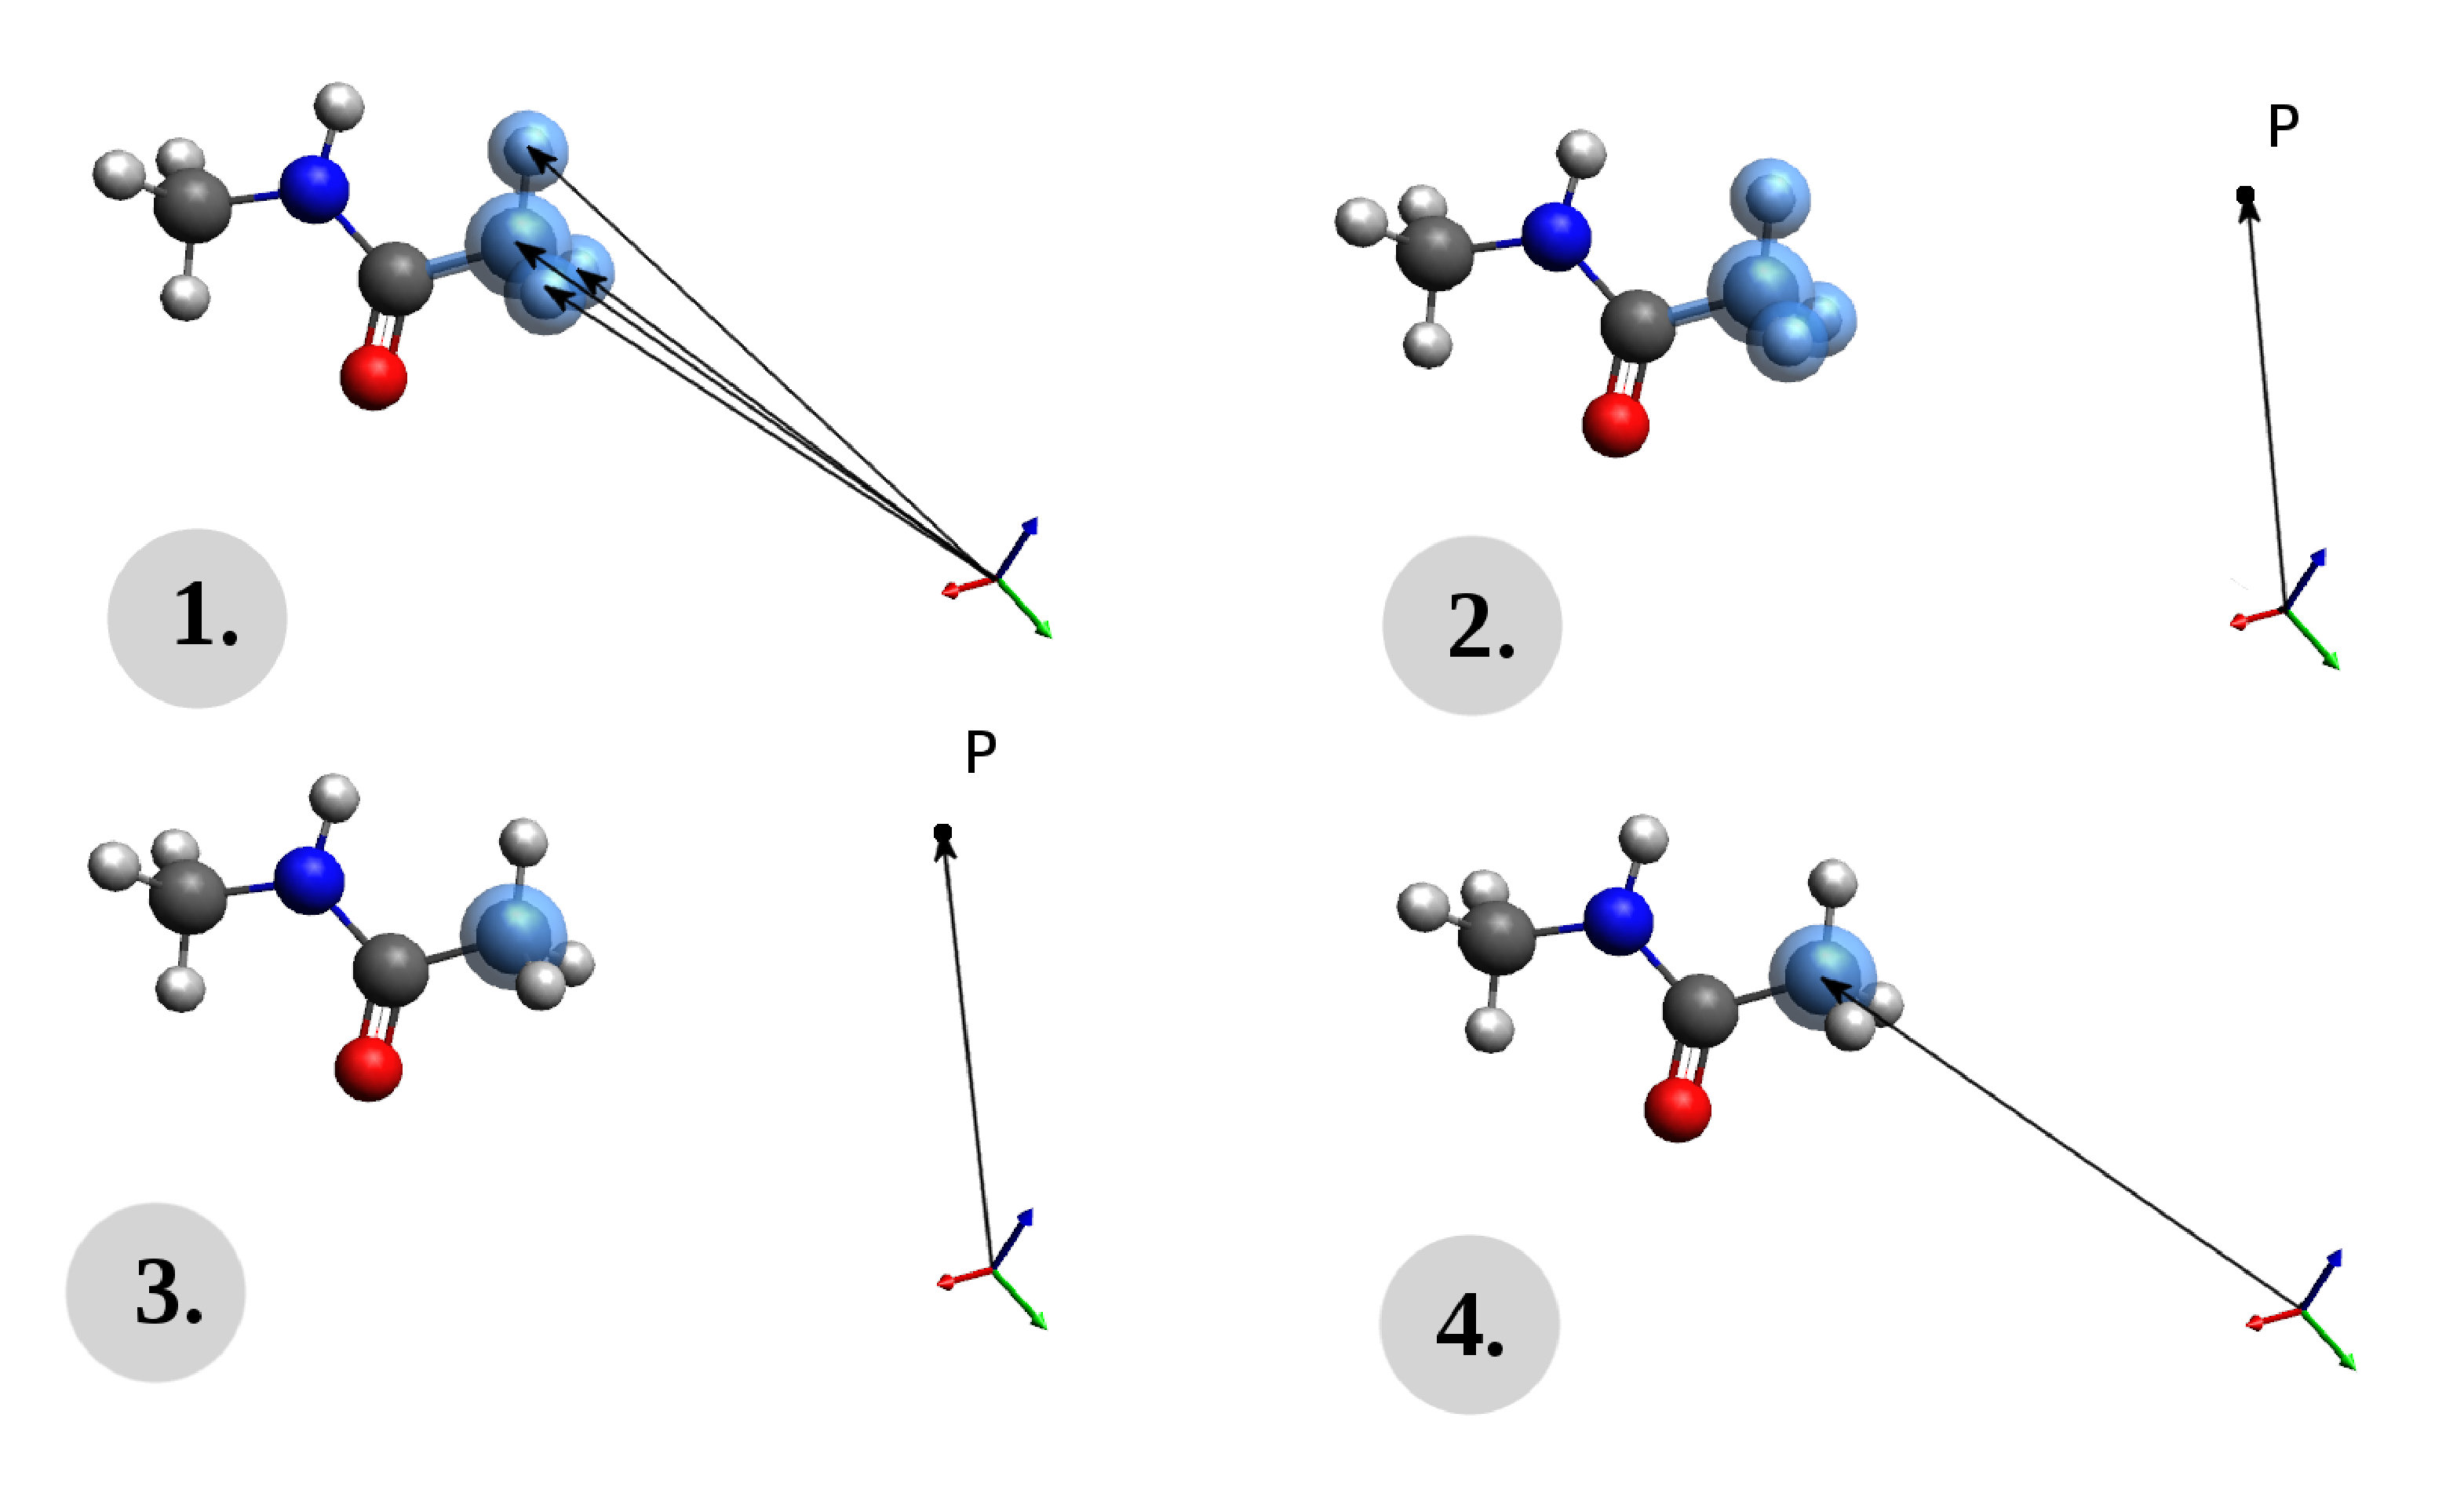
\includegraphics[width=0.1\linewidth]{contr.eps}
%}
%\caption{Performance of SolCAMM-12 (fully distributed) and SolCAMM-6 (two 
%united atoms) for the training set of NMA-H$_2$O$_n=1-30$ clusters.
%\label{f:contr-uncontr-comparison}}
%\end{figure}
%%
%


\printbibliography[heading=subbibintoc,title={References}]
\end{refsection}

% CHAPTER 5 ================================

\begin{refsection}
\chapter{Vibrational Solvatochromism of Amide I Mode\label{c:nma-amide-I}}

Amide I mode which can be thought of C$=$O stretch within
the CONH group in peptides has been studied for long time
in terms of its vibrational solvatochromism because it can
be used to investigate the structure and dynamics of proteins. 
Since it is a good model vibration to start with,
we test our SolEFP and SolEDS theories on the amide I mode
prototypical molecule, $N$-methylacetamide (NMA) dissolved
in a few solvents. We found that, although the Coulombic
contributions to the vibrational frequency shift can approximate
the experimental results, other effects such as induction,
dispersion and exchange\hyp{}repulsion need to be included
for quantitative agreement with experiment, though charge\hyp{}transfer
can be safely neglected. Moreover, we show that the electrostatic
maps developed before worked well because of the strong
orientation\hyp{}dependence of the Coulombic frequency shifts,
in contrast to other contributions. Despite all that, induction,
dispersion and exchange\hyp{}repulsion effects are not at all
weak. In fact, the corresponding contributions to frequency shifts
are very large in magnitude but opposite in sign: induction
and dispersion cause strong red shifts whereas exchange\hyp{}repulsion
causes sharp blue shifts.

\section{Overview}

Amide I mode vibrational frequency (like C$=$O stretches) 
is known for its pronounced
correlation with the external electrostatic potential or
electric field and plenty of electrostatic solvatochromic
ESF maps have been reported up to date. \citep{Hayashi.Zhuang.Mukamel.JPCA.2005,Jansen.Knoester.JCP.2006,
Lee.Choi.Cho.JCP.2012,Torii.JCPL.2015}
However, it is possible that the fitting procedures
can take into account also non\hyp{}electrostatic effects,
unless some maps were free from specific solute\hyp{}solvent
geometry optimisations and frequency analyses,
and have shown to be accurate for polar environments. \citep{Hayashi.Zhuang.Mukamel.JPCA.2005,Jansen.Knoester.JCP.2006}
However, notable disagreement of the line shape and frequency shift was noticed for
non\hyp{}polar solvents such as CHCl$_3$ by Jansen and Knoester \citep{Jansen.Knoester.JCP.2006}
who later refined his study by improving CMD forcefield. \citep{Jansen.JPCB.2014}
It is however noteworthy to realise that in such non\hyp{}polar
environments electrostatic Coulombic interactions are no longer
dominant and other effects can manifest more apparently
in the vibrational solvatochromism. Therefore, application of
SolEDS and SolEFP models could provide critical information
on the general aspect of the vibrational solvatochromism of the amide I modes.

In this Chapter, we first consider model solute\hyp{}solvent
clusters and test the quality of the WCA limit with Onsager theory
and SolEDS model.
We also apply SolEFP theory to those model systems
to directly compare the frequency shifts with exact quantum chemistry
calculations. \citep{Blasiak.Lee.Cho.JCP.2013,Blasiak.Cho.JCP.2014,Blasiak.Cho.JCP.2015} 
Finally, we combine SolEFP with CMD and compare the vibrational
frequency shifts directly with experimental data. \citep{Blasiak.Cho.JCP.2015}
For the detailed computational procedures see the Appendix~\ref{a:computational-details}.
%In general, electrostatics plays the dominant
%role 



\section{Small Model Solute\hyp{}Solvent Clusters}

\subsection{Frequency Shifts from Onsager Model\label{s:amide-I-onsager}}

We start with the testing of the vibrational solvatochromic 
operator $\hat{F}_j$ (Eq.~\eqref{e:dw-fea-fma}) 
for the simples case which is NMA
placed in a spherical cavity of radius $a$ which is surrounded
by continuum medium of dielectric constant $\varepsilon$.
In Chapter~\ref{c:my-model}, we have solved this problem exactly within
WCA limit. 

In the Fig.~\ref{f:onsager} we show the application of the rigid
and flexible vibrational solvatochromism models that are directly
compared with the full QM calculations. It is apparent that WCA
limit is indeed working very well and when the reaction field\hyp{}induced 
structural distortions
are included for the NMA's dipole moment description 
we achieved quantitative agreement
with full QM results. 
%
\begin{figure}[t!]
\centering
\setlength\fboxsep{0.4pt}
\setlength\fboxrule{0.5pt}
\fbox{
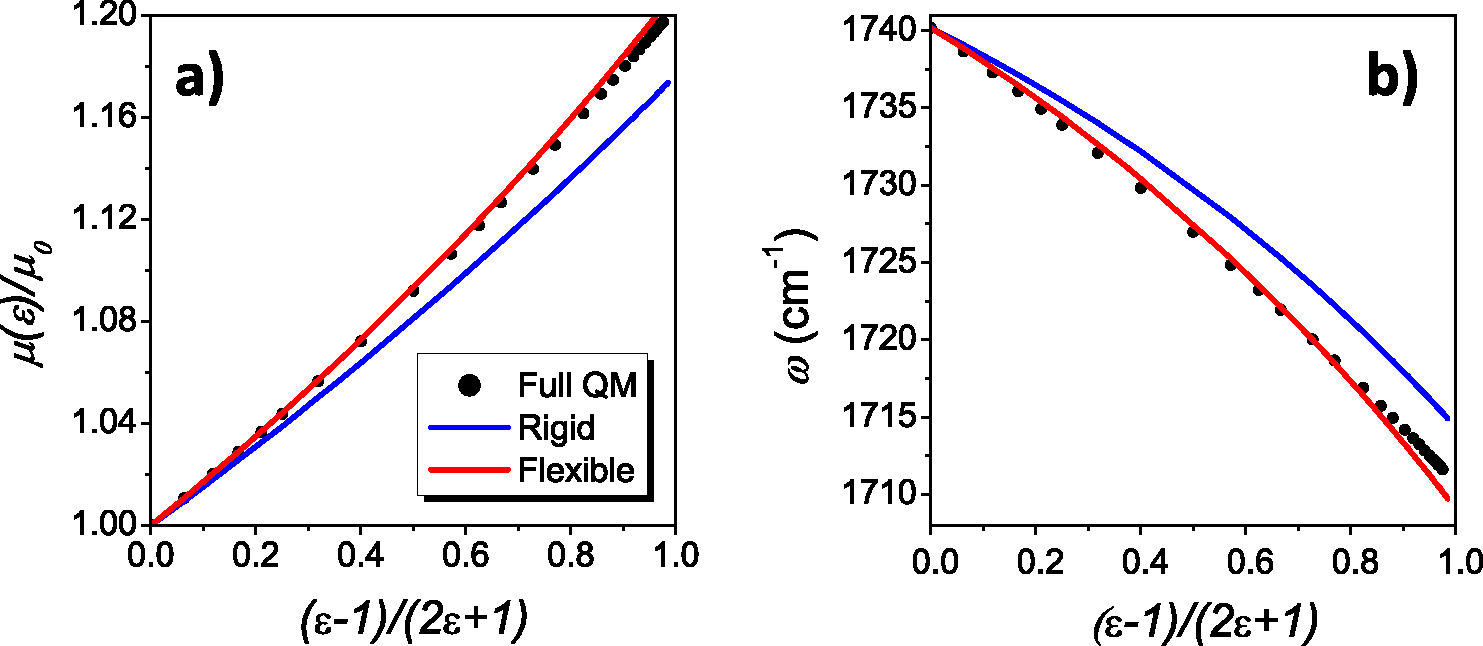
\includegraphics[width=0.97\linewidth]{NMA-Onsager-Freq.eps}
}
\caption{
(a) Ratio of the total NMA dipole moment with respect to its gas\hyp{}phase
value obtained from the DFT/6-311++G** calculation results with rigid and flexible
models (b) The NMA amide I mode frequencies calculated by using the same method
method are compared with the theoretical results using the Onsager model. 
Both rigid and flexible model calculations are shown here. The cavity radius was set
to be 3.72 \AA.
\label{f:onsager}}
\end{figure}
%
Thus, the
iterative algorithm developed in Chapter 4 improves the predicted
dipole moments and reproduces the tangent line at the origin.
However, the qualitative
picture is still well\hyp{}reproduced even if we neglect
structural distortions of NMA molecule. The maximal structural
distortion effect on amide I frequency shift is as small
as $\sim$6 cm$^{-1}$.

\subsection{Frequency Shifts From Solvatochromic Multipoles\label{s:amide-I-solvatochr-multipoles}}

In order to test our solvatochromic SolCAMM, SolMMM and SolChelpG models,
we apply them to various NMA/water clusters
with up to 35 water molecules. Previous attempts \citep{Lee.Choi.Cho.JCP.2012}
to determine the vibrational solvatochromic parameters using the Cho's
coarse\hyp{}grained models were undertaken by considering just the 
vibrational solvatochromic charge\hyp{}electrostatic potential
interaction terms. However, the solvatochromic charges
were determined by carrying out the multivariate
least square fitting analyses of the ab initio or DFT calculated
amide I frequency shifts of NMA in water clusters. 

Here, we compute these
parameters fully from \emph{ab initio} calculations and include also 
higher\hyp{}multipole terms. We apply the following models:
%
\begin{enumerate}
 \item SolX-12 model which includes all the 12 atomic sites of NMA
 \item SolX-6 contracted model which considers 5 heavy atoms (with united
       atom approximation of two methyl groups) and the
       amide hydrogen atom.
 \item SolX-5 contracted model which is derived from SolX-6 by treating N--H
       as a united atom at the nitrogen atom.
\end{enumerate}
%
In the above, X denotes MMM, CAMM and ChelpG methods. 

\subsubsection{Rigid Molecule Algorithm\label{s:rigid-molecule-algorithm}}

Once these distributed vibrational solvatochromic
charges and multipoles are calculated, one should properly
place them on a given NMA molecule in either NMA/water
clusters or CMD simulation trajectories for subsequent calculations
of amide I frequency. However, there are certain
difficulties. In general, there is no unique transformation matrix from the gas\hyp{}phase
structure to a target structure of solute (and solvent) molecule
because the molecular structures in solution
undergo a continuous fluctuation in time.
Therefore, the transferring the gas\hyp{}phase molecular
properties onto the target structure
is not straightforward at all, especially in the cases of vibrational
solvatochromic multipoles because of their tensorial nature.
Therefore, we needed to assume that molecular
structure changes induced by solvation are negligibly small
at least for the backbone atoms of NMA. Only then, it
becomes possible to develop three\hyp{}stage rigid\hyp{}molecule
algorithm:
%
\begin{enumerate}
 \item {\bf Superimposition:} The first step is to obtain
the rotation matrix minimising the root mean square (RMS) deviation
between the gas\hyp{}phase and target molecular structure. 
In the present study, the rotation matrix $\bf R$ is calculated
by using the Kabsch algorithm. \citep{Kabsch.ActCrystSecA.1976} 
From the singular value decomposition
(SVD) of the covariance matrix constructed from the reference and target
molecular geometries as ${\bf C} = {\bf r}^T {\bf r}_0$ (where ${\bf r}_0$
and ${\bf r}$ are
the molecular structures of the reference and target, respectively) we compute
the optimal rotation matrix $\bf R$ as
 %
 \begin{equation}
  {\bf R} = {\bf W} 
 \begin{bmatrix}
1  & 0 & 0\\ 
0  & 1 & 0\\ 
0  & 0 & d
\end{bmatrix}
  {\bf V}^T
 \end{equation}
 %
where $d={\rm sign}\;\det{({\bf W}{\bf V}^T)}$ and SVD matrices are defined as 
${\bf C}\overset{{\rm SVD}}{=} {\bf V}{\BM \Sigma}{\bf W}^T$.
 %
 \item {\bf Translation:} Since the origin for multipole moments
of an isolated NMA can be different from that of
target molecule, they should be translated properly. Such
translation of (distributed) primitive multipole moment
origin from ${\bf r}_i = {\bf 0}$ to a new origin at ${\bf r}_i$ is made by using
the following formula:
  %
 \begin{equation}
 M_{klm}({\bf r}_i) = M_{klm}({\bf 0}) - \sum_{k'\ge 0}^{k\ne k'} 
                                         \sum_{l'\ge 0}^{l\ne l'} 
                                         \sum_{m'\ge 0}^{m\ne m'}
 \begin{pmatrix}
k\\k' 
\end{pmatrix}
\begin{pmatrix}
l\\l' 
\end{pmatrix}
\begin{pmatrix}
m\\m' 
\end{pmatrix}
 x_i^{k-k'} y_i^{l-l'} z_i^{m-m'} M_{k'l'm'}({\bf r}_i)
 \end{equation}
 %
Note that this step is performed when we want to
change the origin of multipoles in local molecular coordinate
frame. In the case of the SolCAMM method\footnote{and also SolMMM, since it is
a limiting case of SolCAMM, i.e., recentered to the same origin and summed over},
there is no need to go through this step because the distributed
multipoles are located at atomic sites. However,
the same translation procedure has to be performed to
create the contracted SolCAMM parameters with united
atom approximation. 
 %
 \item {\bf Rotation:} With the rotation matrix $\bf R$ obtained
from Step 1, the tensorial multipoles can be properly
rotated, i.e.,
 %
 \begin{equation}
 M_{ijk\ldots}' = \sum_{i'j'k'\ldots} R_{ii'} R_{jj'} R_{kk'} \ldots M_{i'j'k'\ldots}
 \end{equation}
 %
\end{enumerate}
%
Now, to calculate the solvent electric field and its gradients
on the solute molecule, the same procedure is performed
for each solvent molecule with benchmark solvent molecule
(BSM) distributed multipole moments. For the sake of simplicity,
we neglect the structural changes of water molecules
as usual because the vibrational properties of solute are of
our concern. The algorithm proposed here could be improved
to some extent by making it more flexible, i.e., by considering
the rotation matrices between respective fragments like
the two methyl groups and O$=$C$-$N$-$H amide group of NMA
in an \emph{ad hoc} manner. 
Nevertheless, the estimated RMS values for all the
cases were less than 0.07 a.u. for NMA and 0.04 a.u. for water
molecules. Therefore, we believe that, for the purpose of
the present study, this approximate algorithm is sufficiently
accurate and acceptable.

\subsubsection{Frequency Shifts from Molecular Multipole Moments}

As the crudest approximation studied here, we consider 
the vibrational solvatochromism model based on calculated
molecular multipole moments that are calculated with respect to
the centre of square eigenvector element
defined as
%
\begin{equation} \label{e:coe}
 {\bf R}_{\rm COE}^{(j)} \equiv 
 \sum_m \left\{ (L^{(j)}_{m;x})^2 + (L^{(j)}_{m;y})^2 + (L^{(j)}_{m;z})^2\right\} {\bf r}_m
\end{equation}
%
where $m$ denotes atomic site and $L^{(j)}_{m;x}$ is the $x$th
element of the mass\hyp{}weighted vibrational eigenvector
referring to the $j$th normal mode.
First, we have compared the SolMMM moments up to octupoles
with previously determined solvatochromic multipoles
constructed from the vibrational solvatochromic charges
according to the following relations \citep{Lee.Choi.Cho.JCP.2012}:
%
\begin{subequations}
\begin{align}
 L_{j;\alpha}                  &= \sum_x l_{j,x} r_{x;\alpha} \\
 \Lambda_{j;\alpha\beta}       &= \sum_x l_{j,x} \left( 3r_{x;\alpha}r_{x;\beta} - r_x^2 \delta_{\alpha\beta}\right) \\
 \lambda_{j;\alpha\beta\gamma} &= \sum_x l_{j,x}\left( 5r_{x;\alpha}r_{x;\beta}r_{x;\gamma} - r_x^2 \left[
                    r_{x;\gamma}\delta_{\alpha\beta} + r_{x;\beta}\delta_{\alpha\gamma} + r_{x;\alpha}\delta_{\beta\gamma}\right]\right)
\end{align}
\end{subequations}
%
We note that $l_{j,x}$ parameters were obtained from fitting procedure
to the electrostatic potential evaluated
at six atomic sites of NMA-$d$ to reproduce the benchmark frequency shifts 
from the formula
%
\begin{equation}
 \Delta\omega = \sum_{x=1}^6 l_{j,x} \phi({\bf r}_x)
\end{equation}
%
The results are shown in Table~\ref{t:solmmm-comparison}.
%
\begin{table}[t]
\caption{
Vibrational solvatochromic molecular multipole moments (SolMMM) 
for NMA-$d$ obtained by using 
B3LYP/6-311++G** method. Here the origin
of the molecule\hyp{}fixed coordinate frame is at the centre of 
square eigenvector element
(COE). Thus obtained vibrational solvatochromic multipoles are 
directly compared with
those obtained from the multivariate least\hyp{}square fitted 
distributed solvatochromic charges for a large collection of 
NMA-$d$/water clusters. \citep{Lee.Choi.Cho.JCP.2012} Vibrational
solvatochromic dipole, quadrupole, and octupole moments are given 
in cm$^{-1}$/(MV/cm), 10$^{-8}$ cm$^{-1}$/(MV/cm$^2$), and 
10$^{-16}$ cm$^{-1}$/(MV/cm$^3$), respectively. The
definitions of the traceless quadrupole and octupole moments 
as well as the orientation of NMA-$d$ molecule were taken from Ref.~\citep{Lee.Choi.Cho.JCP.2012}
\label{t:solmmm-comparison}}
\begin{tabular*}{1.0\textwidth}{@{\extracolsep{\fill} } l l l l l l l l }
\hline\hline
 &     \multicolumn{2}{c}{Dipole}  & & \multicolumn{4}{c}{Quadrupole} \\
 &  x    & z   & & xx & xz & yy & zz \\
Ref.~\citep{Lee.Choi.Cho.JCP.2012} & -0.04 & -1.19 && 2.72 & 0.56 & -3.96 & 1.24 \\
This work                          & 0.32  & -0.67 && 5.43 & 1.17 & -1.89 & -3.54 \\
 & \multicolumn{7}{c}{Octupole} \\
 & xxx & zzz & xxz & yyx & yyz & zzx & \\
Ref.~\citep{Lee.Choi.Cho.JCP.2012} & -2.94 & 7.22  & -10.86 & 3.53 & 3.64 & -0.59 & \\
This work                          &  7.33 & 2.58  & -1.25  &-5.94 &-1.32 &- 1.39 & \\
\hline\hline
\end{tabular*}
\end{table}
%
The orientation of NMA-$d$ was such that the $z$-axis was taken to
be collinear with the C$=$O bond and the O$=$C$-$N group lies on
the $xz$ plane. Therefore, all the components containing odd number of 
$y$ indices (e.g., $xy$ component of quadrupole and $yyy$ component of octupole)
were zero or
vanishingly small.

We find that the SolMMM tensor elements
obtained by using the two different approaches appear to be
different from each other. The solvatochromic dipole obtained
using the multivariate fitting analyses is almost parallel to
the C$=$O bond, whereas the present fully \emph{ab initio} SolMMM dipole moment
has considerably large $x$-component and forms the angle of
25.5\textdegree with respect to the $z$-axis (C$=$O bond axis). 
In addition,
the magnitudes and signs of respective quadrupole and
octupole tensor elements appear to be different as well. 
Interestingly,
despite these relatively large differences between the
two sets of vibrational solvatochromic multipoles, the corresponding
vibrational amide I' mode frequency shifts are found
to be in very good agreement with each other and the predictions
made by these models are similar which are plotted in Fig.~\ref{f:solmmm}b.

Let us analyse the convergence properties of SolMMM vibrational
frequency shifts.
The asymptotic distance dependence of the interaction between
two multipoles of rank $n_1$ and $n_2$ is equal to $R^{-(n_1+n_2+1)}$
where $R$ is the distance between the multipole origins.
For instance, the $R^{-n}$\hyp{}dependence of the dipole\hyp{}quadrupole
interaction is $R^{-4}$, or in other words, this interaction decays asymptotically
as $R^{-4}$ when $R$ increases. It is useful to classify all the terms in the
expansion of the Coulombic interaction energy (and frequency shift)
according to their $R^{-n}$\hyp{}dependencies and study the convergence
by including terms with larger $n$. In Fig.~\ref{f:solmmm} we depict the
vibrational frequency shifts of amide I (I') modes in water
correlated with the full DFT results.
%
\begin{figure}[t!]
\centering
\setlength\fboxsep{0.4pt}
\setlength\fboxrule{0.5pt}
\fbox{
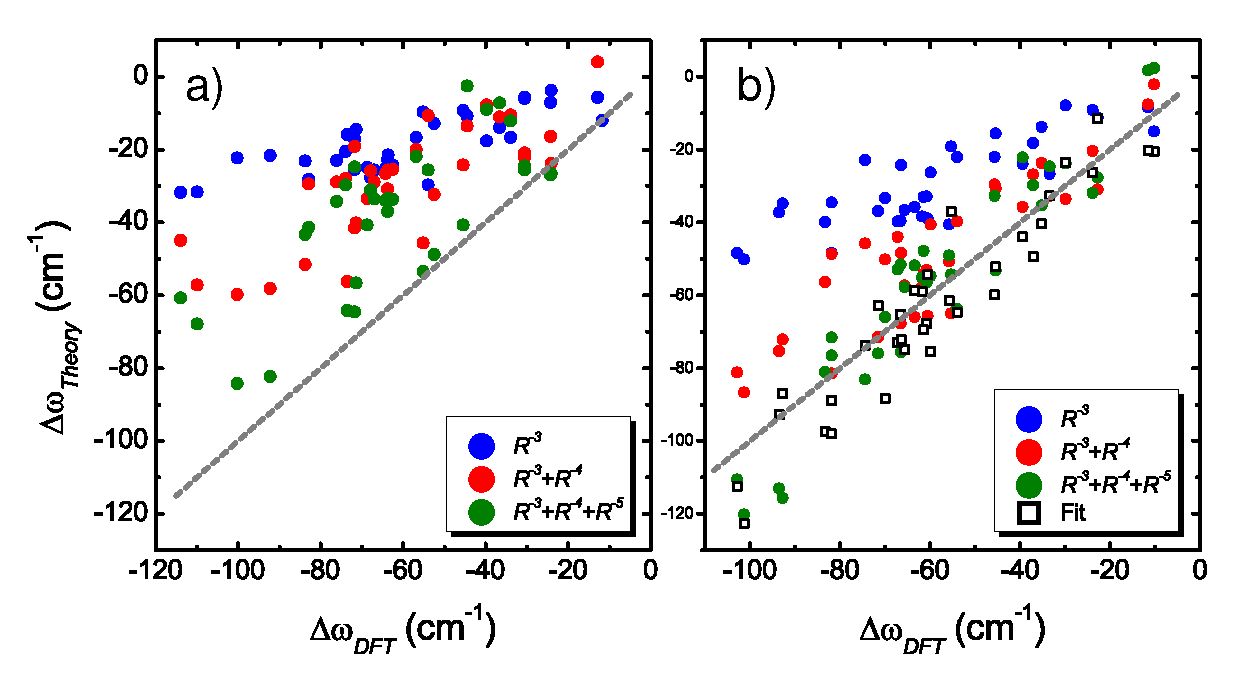
\includegraphics[width=0.97\linewidth]{NMA-SolMMM-COE.eps}
}
\caption{
Amide I and I' harmonic frequency shifts of NMA (a) and NMA-$d$ (b) 
are compared with the B3LYP/6-311++G**/SolMMM(COE) coarse\hyp{}grained
model results. In the case of NMA-$d$ (b) the frequency shifts obtained 
by using solvatochromic molecular multipole moments from Ref.~\citep{Lee.Choi.Cho.JCP.2012} 
are also shown (see black squares). Here, the convergence of multipole expansion 
is examined by calculating interaction energies and vibrational frequency shifts 
that are summed up to $R^{-3}$ (blue), $R^{-4}$ (red), and $R^{-5}$ (green) terms, 
respectively.
\label{f:solmmm}}
\end{figure}
%
In most of the cases of the NMA amide I mode, the predicted
shifts appeared to diverge when the dipole\hyp{}quadrupole
interactions are taken into account. 
There is a noticeable correlation only for the
dipole\hyp{}dipole interactions ($R^{-3}$ terms).
This is in contrast to the amide I'\hyp{}mode frequency shifts of
NMA-$d$, where we observe acceptable convergence when
even dipole\hyp{}octupole and quadrupole\hyp{}quadrupole
interactions are included.
This difference in convergence
when the SolMMM model is applied for NMA and
NMA-$d$ molecules can be understood by considering the isotopic
effect on amide I mode. Substitution of amide hydrogen
atom by deuterium makes the NMA-$d$ amide I' mode more localised
on carbonyl group because deuterium is heavier than prot. 
Thus, the vibrational solvatochromic charge
density is more localised in space and, therefore, the effective
size of vibrational probe is smaller. 
But it means that the divergence sphere
of multipole expansion is smaller as well. 

However, in the case of NMA,
the methyl groups and amide proton centre are also important for a solvatochromic
response and one\hyp{}centre model cannot capture the atomic
granularity of a molecule. Thus, it is clear that, in general,
the one\hyp{}centred multipole SolMMM model is not suitable in
practical applications because of possible problem of convergence.
In addition, SolMMM moments strongly depend on the choice of the
origin \citep{Lee.Choi.Cho.JCP.2012} which makes the application
of SolMMM more difficult.
Thus, we conclude that the distributed\hyp{}interaction site
models should be generally used.

\subsubsection{Frequency shifts from distributed multipoles}

Let us focus on SolChelpG and SolCAMM approaches. Both involve multipoles
that are distributed on atoms. However, SolChelpG scheme is approximate
because each ChelpG charge is obtained from fitting to reproduce the electrostatic
potential. Therefore, numerical differentiation of ChelpG charges
contains errors that are difficult to estimate quantitatively.

In Fig.~\ref{f:solchelpg} we plot the corresponding SolChelpG-12, SolChelpG-6 and
SolChelpG-5 vibrational frequency shifts for both NMA and NMA-$d$.
Panels (c) and (f) in this figure show the most accurate estimations
in which both mechanical and electric anharmonicities are included.
Apparently, the results are far from the benchmark DFT frequencies.
On the other hand, the SolChelpG results are clearly in correlation
with the benchmark. Lack of the full agreement can be cause either
by the neglect of other interactions or by errors introduced into
the SolChelpG scheme when numerical differentiation is performed.
%
\begin{figure}[t!]
\centering
\setlength\fboxsep{0.4pt}
\setlength\fboxrule{0.5pt}
\fbox{
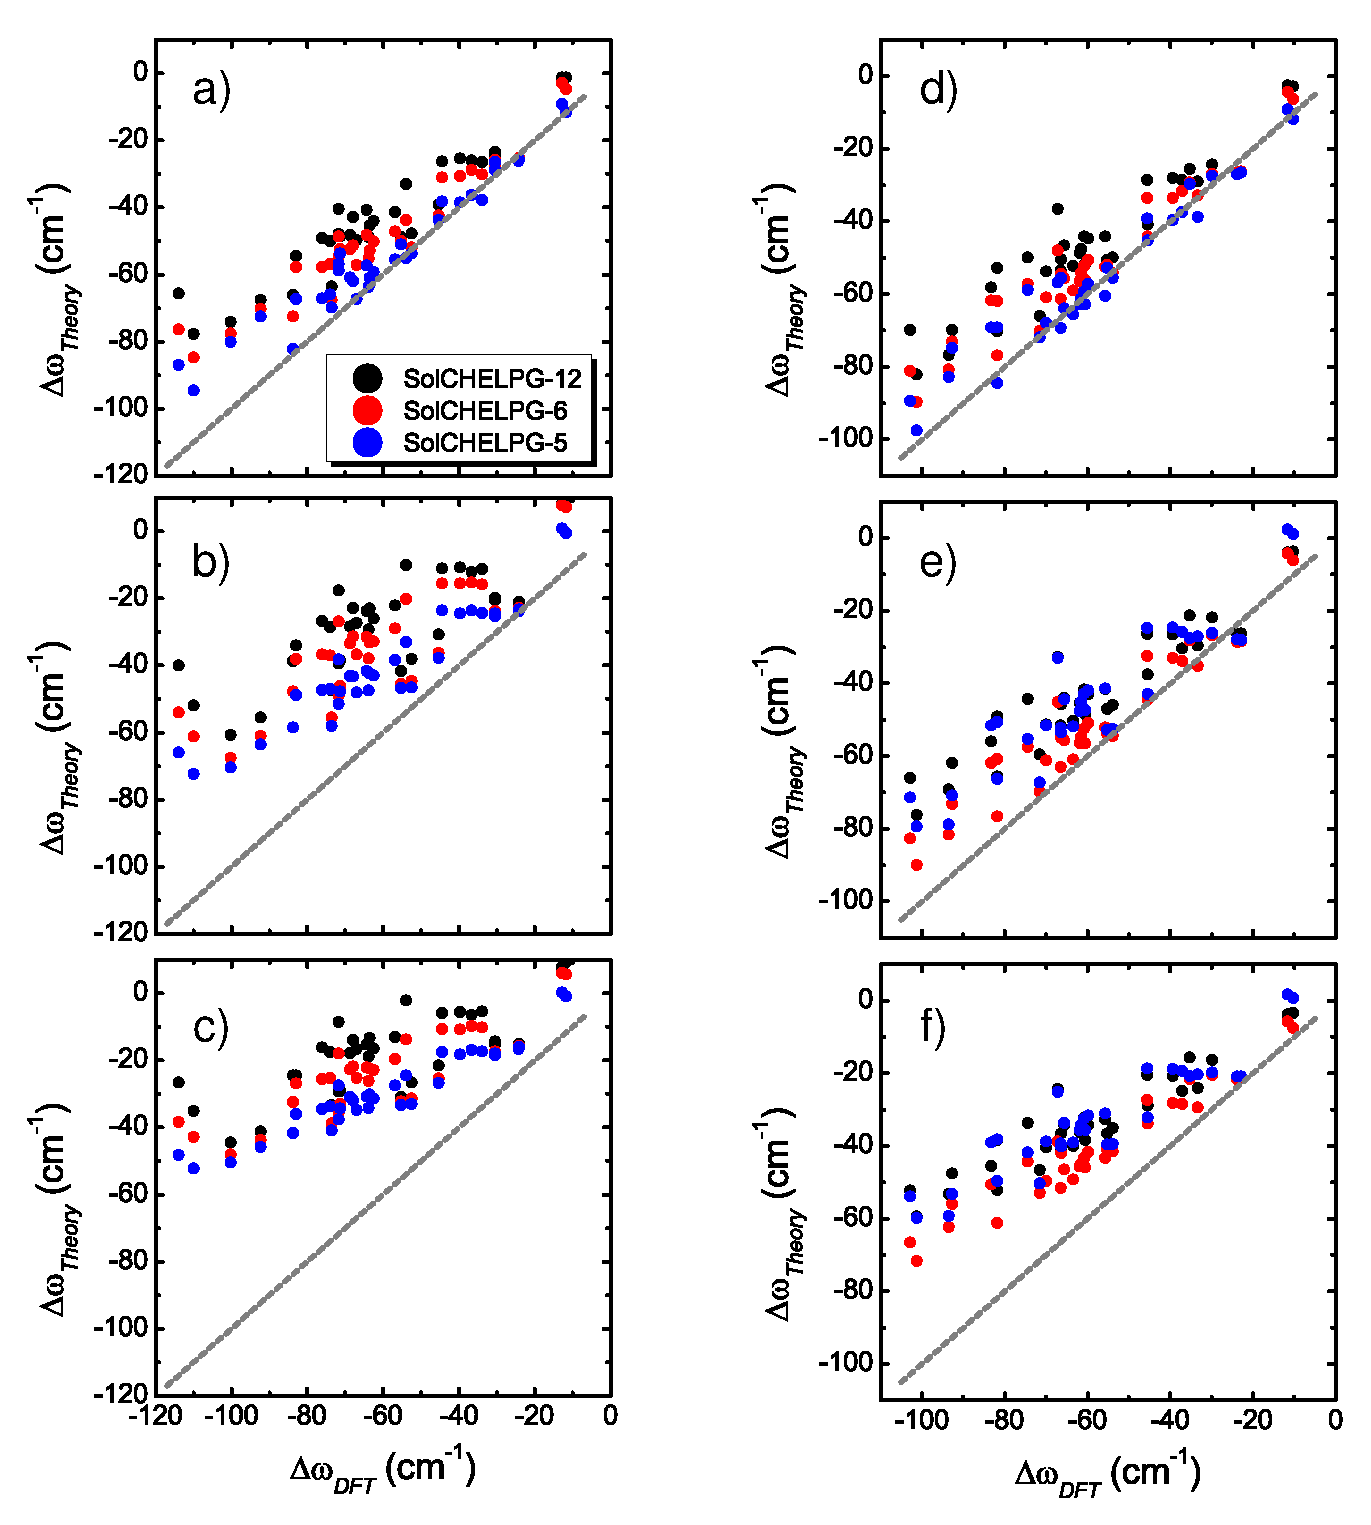
\includegraphics[width=0.97\linewidth]{NMA-SolCHELPG.eps}
}
\caption{
Harmonic frequency shifts of amide I mode of NMA (a-c) and amide II mode
of NMA-$d$ (d-f) calculated using
B3LYP/6-311++G**/SolChelpG (n = 12, 6, and 5) coarse\hyp{}grained model
are compared with full DFT results. (a) and (d) Mechanical anharmonicity with the
diagonal cubic anharmonic constant only; (b) and (e) mechanical anharmonicity with
all the diagonal and off\hyp{}diagonal cubic anharmonic constants included; and
(c) and (f) both mechanical and electronic anharmonicities.
\label{f:solchelpg}}
\end{figure}
%

It is also instructive to examine the importance of the
mechanical and electric anharmonicities. In previous works
the following assumption was made
%
\begin{equation} \label{e:approx-1}
 \Delta \omega_j \approx -\frac{g_{jjj}}{2M_j^2\omega_j^3} \fderiv{U}{Q_j} 
                 \approx -\frac{g_{jjj}}{2M_j^2\omega_j^3} \sum_x \fderiv{q_x}{Q_j} \phi({\bf r}_x)
\end{equation}
%
which defines the solvatochromic charge $l_x\equiv-\frac{g_{jjj}}{2M_j^2\omega_j^3} \fderiv{q_x}{Q_j} $.
This is because it was difficult to compute all the derivatives 
directly.
Thus, by finding $l_x$ by fitting to benchmark frequencies, 
the charge\hyp{}flow terms were inferred that tell about the
response of the particular IR probe's atomic site against the external electric field.
However, this approximation neglects off\hyp{}diagonal cubic anharmonic
constants $g_{ijj} \text{for $i\ne j$}$. Also, this neglects $\sderiv{U}{Q_j}$
which contributes to the electric anharmonicity. Our SolChelpG analysis
can estimate the importance of these neglected previously factors.

In Fig.~\ref{f:solchelpg}a and \ref{f:solchelpg}d the results of estimating Eq.~\eqref{e:approx-1} are shown.
There is an accidental agreement with the benchmark DFT results.
When we used the following approximation
%
\begin{equation} \label{e:approx-2}
 \Delta \omega_j \approx -\frac{1}{2M_j\omega_j} \sum_i \frac{g_{ijj}}{M_i\omega_i^2}\fderiv{U}{Q_i} 
\end{equation}
%
which is shown in Fig.~\ref{f:solchelpg}b and \ref{f:solchelpg}e, certain deterioration of the SolChelpG
performance is found. Finally, when the electric anharmonicity is
included
%
\begin{equation} \label{e:approx-3}
 \Delta \omega_j \approx \frac{1}{2M_j\omega_j} \left[
 \sderiv{U}{Q_j} -
 \sum_i \frac{g_{ijj}}{M_i\omega_i^2}\fderiv{U}{Q_i} 
\right]
\end{equation}
%
the results are even worse. Thus it is clear that both electric anharmonicity
and off\hyp{}diagonal cubic anharmonic constants need to be properly taken into
account. Also it is evident that the SolChelpG method does not work quantitatively
correct.

The most accurate model is to use
distributed multipole analysis method such as SolCAMM
which is also free from numerical differentiation errors,
in contrast to SolChelpG method.
In Figs.~\ref{f:solcamm} we present the SolCAMM-6 results 
for amide I and I' modes. It is clear that
these models work very well and the predicted 
vibrational frequency shifts are in fairly good correlation
with benchmark DFT calculations, though in the case of NMA-$d$
the red shifts are somewhat overestimated.
It is also apparent that SolCAMM-6 results are
convergent in both amide I and I' mode cases, which is
an improvement over single\hyp{}centred SolMMM method.
%
\begin{figure}[t!]
\centering
\setlength\fboxsep{0.4pt}
\setlength\fboxrule{0.5pt}
\fbox{
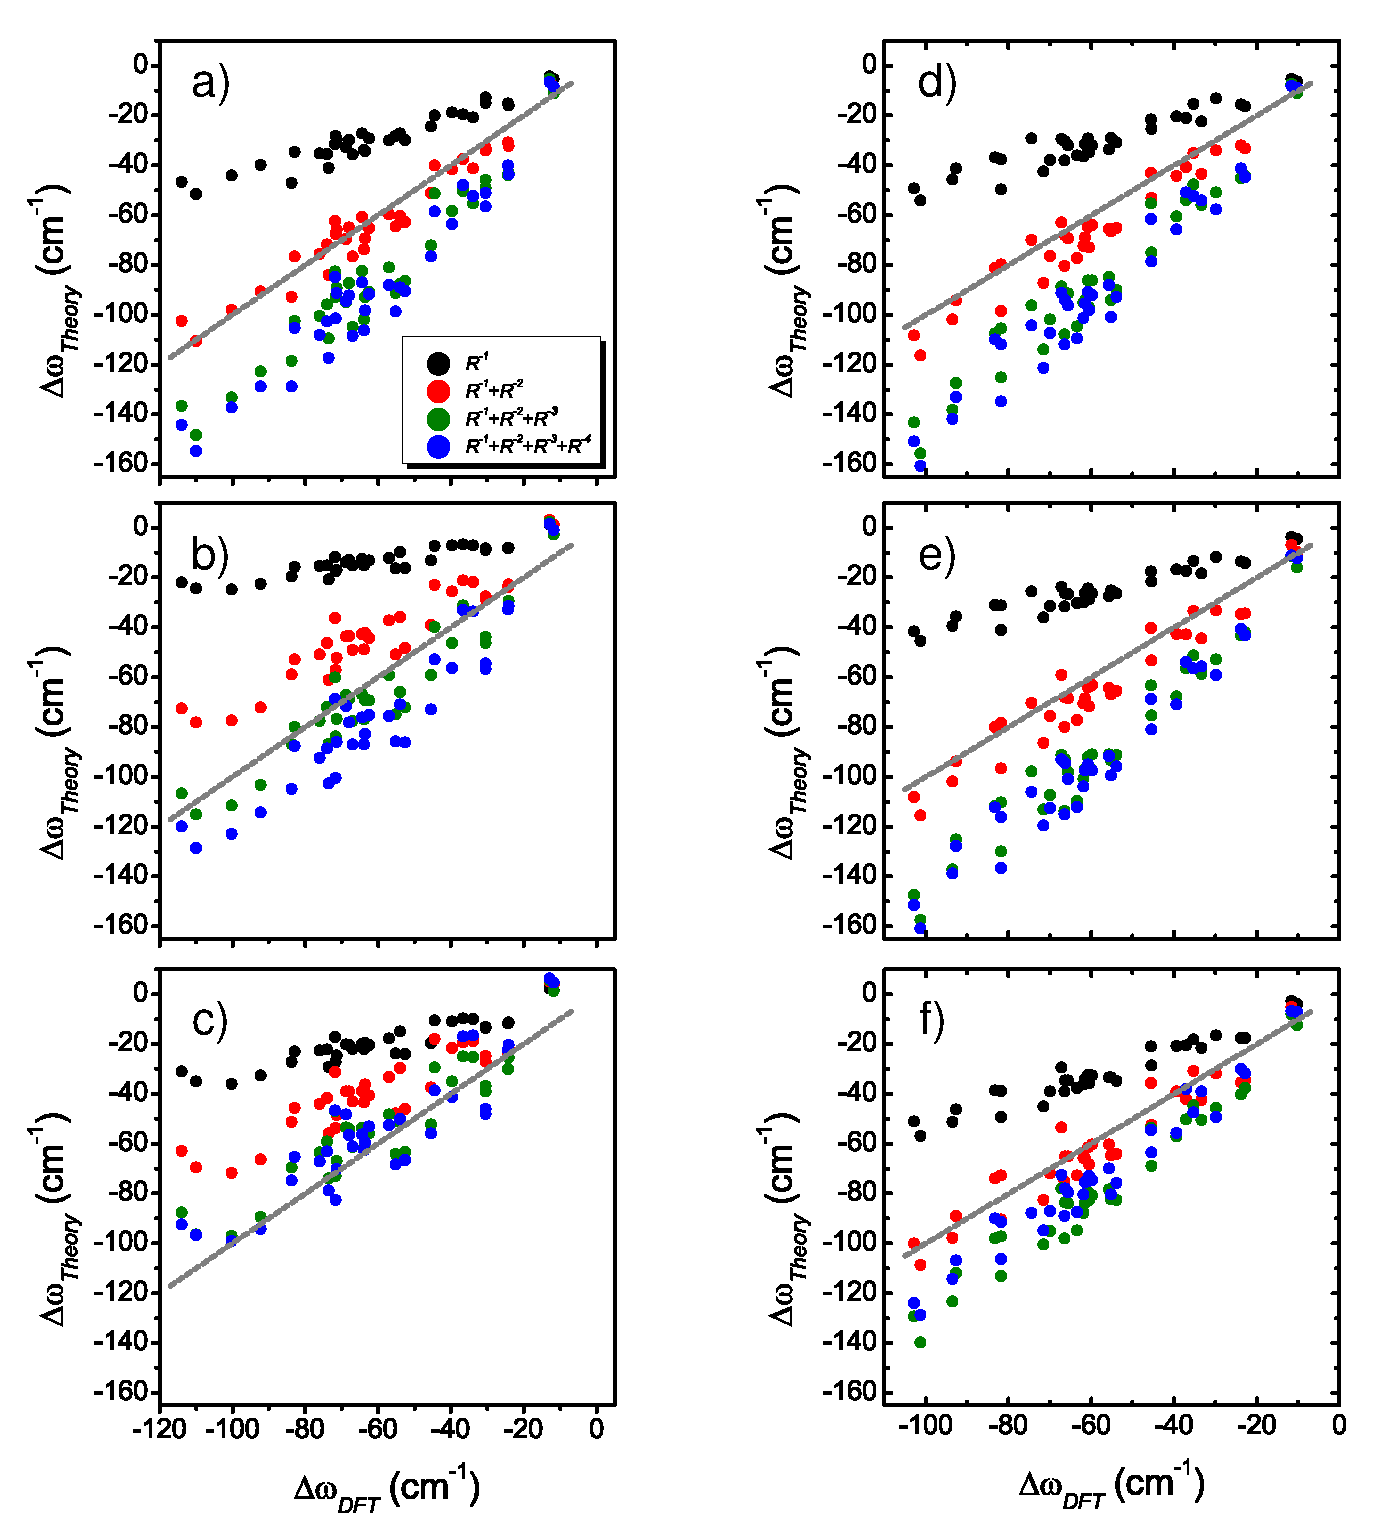
\includegraphics[width=0.97\linewidth]{NMA-SolCAMM-6.eps}
}
\caption{
Harmonic frequency shifts of amide I mode of NMA (a-c) and amide II mode
of NMA-$d$ (d-f) calculated using
B3LYP/6-311++G**/SolCAMM-6 coarse\hyp{}grained model
are compared with full DFT results. (a) and (d) Mechanical anharmonicity with the
diagonal cubic anharmonic constant only; (b) and (e) mechanical anharmonicity with
all the diagonal and off\hyp{}diagonal cubic anharmonic constants included; and
(c) and (f) both mechanical and electronic anharmonicities.
The convergence of multipole
expansion is examined by calculating interaction energies and vibrational frequency
shifts that are summed up to $R^{-1}$ (black), $R^{-2}$ (red), $R^{-3}$ (green), and
$R^{-4}$ (blue) terms, respectively.
\label{f:solcamm}}
\end{figure}
%

Now we can re-investigate also the accidental good SolChelpG performance under the
approximation Eq.~\eqref{e:approx-1}. We performed similar 
calculations with the SolCAMM-6 method and found that when only $g_{jjj}$
constants are included in the mechanical anharmonicity term, 
the resulting vibrational frequency red shifts are strongly overestimated.
This is still the case when also off\hyp{}diagonal cubic anharmonicity
is taken into account but without electric anharmonicity.
Thus, it is believed that a lack of adequate description
of electrostatic potential distribution in the SolChelpG
model might cause such an accidental agreement with full DFT results. Furthermore,
as in the case of SolChelpG model, mechanical
anharmonicities are negligible for amide I' mode shifts -- note
that the data in Fig.~\ref{f:solcamm}d are almost identical to those in
Fig.~\ref{f:solcamm}e.

Before we close this Section, it is worth discussing 
the performance of contracted SolChelpG and
SolCAMM models. As can be seen in Fig.~\ref{f:solchelpg}, 
the reduction of the number of distributed centres
does not influence much the performance of the methods, even if united atom 
model on nitrogen is created (resulting in just 5 distributed centres). 
This fact can be used to reduce the computational cost of the method
and the contracted models can be safely applied (at least for NMA amide I mode).
Thus, from computational point of view SolCAMM-6 is the best of the methods
presented here (we prefer to include amide proton just in case).

\subsection{Beyond Coulombic Approximation}

Thus far we have elaborated on the accuracy and computational
feasibility of using Coulombic models of the vibrational solvatochromism.
Now let us study also other effects in detail.
First we focus on the HF approximation
so that it is possible to directly compare SolEFP calculations
with SolEDS and full QM analysis results. The role of intermolecular dispersion interaction
will be discussed later because it is virtually absent
at HF level of theory. Also, we analyse the other electron correlation
effects by using SolEDS//MP2 method. The orientation\hyp{}
and distance\hyp{}dependencies of the various contributions
to the frequency shifts are further studied to elucidate on
the ranges of Coulombic, induction, dispersion and exchange\hyp{}repulsion
effects on the vibrational solvatochromism of amide I mode.
Finally, we challenge with modelling the bulk solutions
and confront our SolEFP model with experiment.

\subsubsection{Hartree-Fock Approximation}

To gain deeper insight into the origin of the frequency
shift of NMA amide I mode, we first analysed the three simple
NMA--water dimers A, B and C, and the NMA--CHCl$_3$ dimer D 
shown in Fig.~\ref{f:nma-abcde}. 
%
\begin{figure}[t!]
\centering
\setlength\fboxsep{0.4pt}
\setlength\fboxrule{0.5pt}
\fbox{
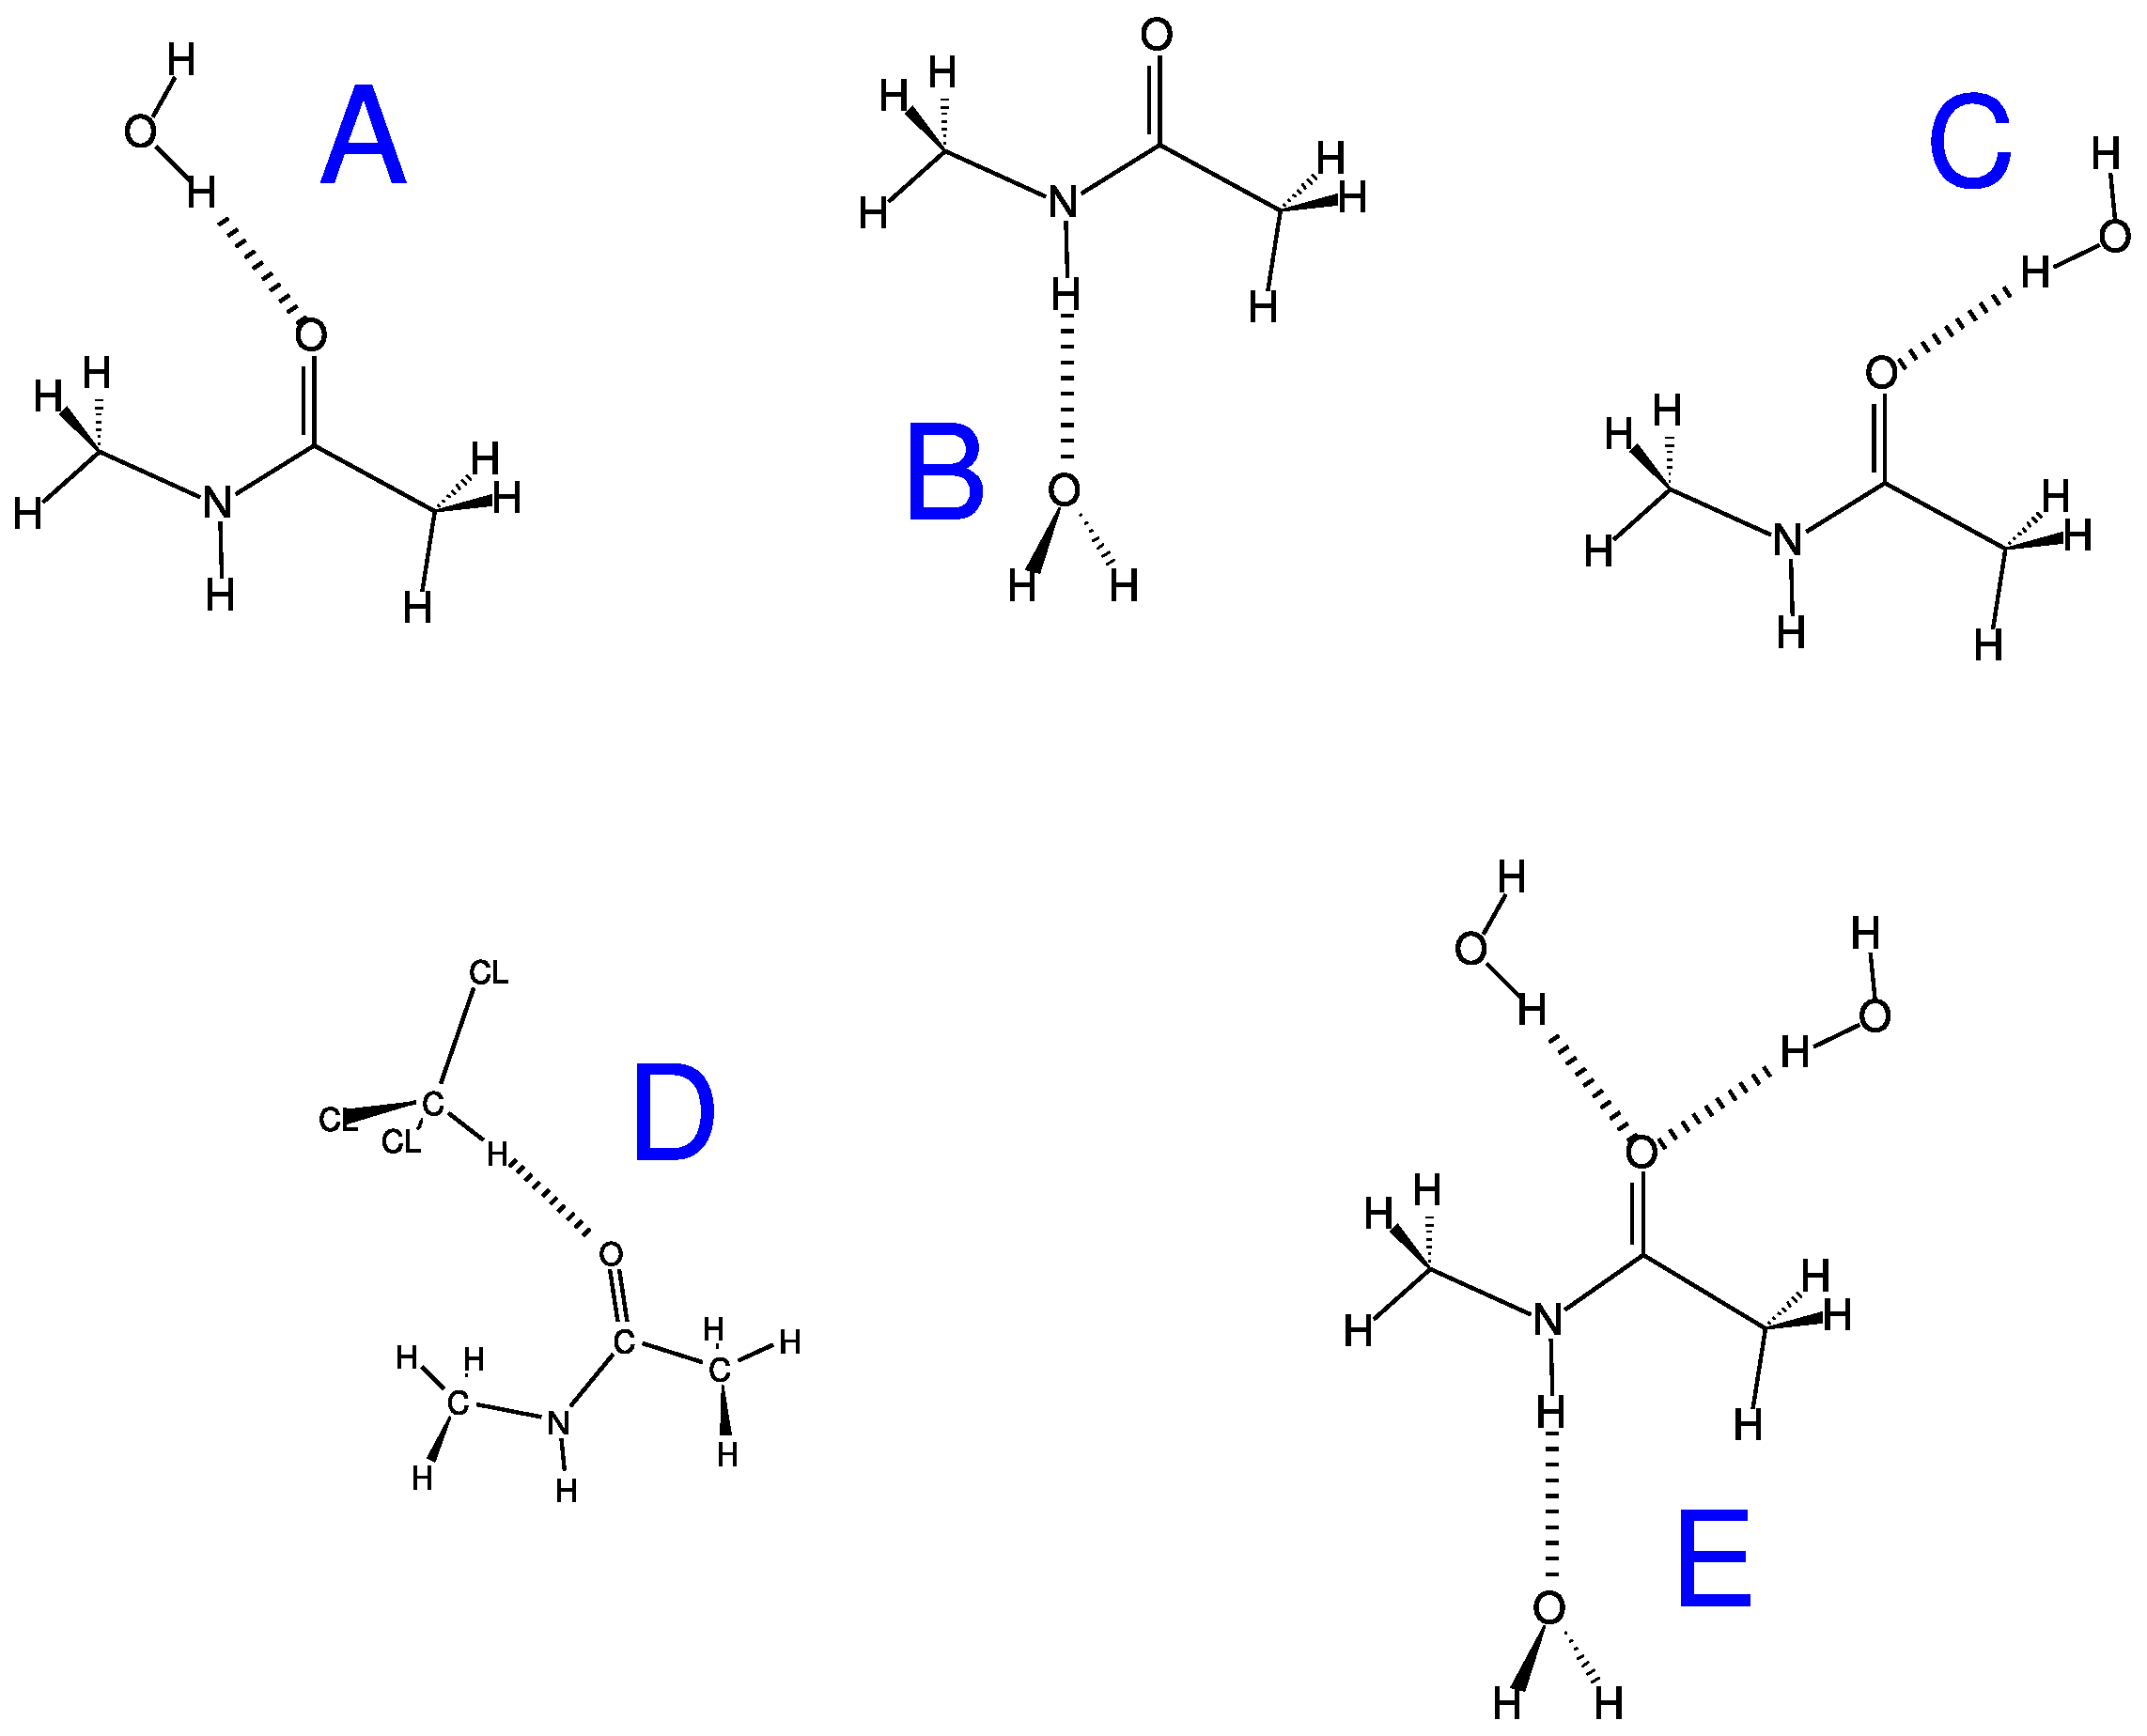
\includegraphics[width=0.97\linewidth]{NMA-ABCDE.eps}
}
\caption{
Model NMA--(H$_2$O)$_{n = 1,3}$ and NMA--CHCl$_3$ clusters 
for SolEDS and SolEFP analyses. The NMA has three H-bonding sites so that three dimers A, B, and C are
considered here. In addition, to examine the many\hyp{}body effects on polarization contribution 
to the amide I frequency shift, we also carried out quantum
chemistry calculations for the NMA with three H-bonded water molecules in configurations
AB, AC and BC.
\label{f:nma-abcde}}
\end{figure}
%

The frequency
shifts evaluated by using (i) constrained\hyp{}cluster\footnote{See Appendix~\ref{a:constrained-models} for details about
the constrained cluster method used here} SolEDS and
SolEFP methods and (ii) analytical SolEFP equations applied
for the fully optimised clusters are summarised in Table~\ref{t:amide-I-soleds-solefp}.
%
\begin{table}[t!]
\caption{
SolEDS and SolEFP results (HF/6-311++G**) 
on amide I frequency shifts of either constrained or unconstrained NMA--H$_2$O% and NMA--CHCl$_3$ dimers
shown in Figure~\ref{f:nma-abcde}. 
Constrained calculations
utilised numerical evaluation of interaction potential derivatives with respect to (wrt) normal coordinates of NMA whereas unconstrained calculations were
based on analytical SolEFP formulae. All the components contributing to the amide I frequency shift are separately
estimated for the sake of comparison. Also, not only the contribution from the mechanical anharmonicity (MA) term but also that from both MA and electric
anharmonicity (EA) terms are given in this table. The negligible contributions to frequency shifts which were not implemented in SolEFP scheme are denoted
as “n.i.” Those components that were not determined are indicated
as “n.d.” Full QM (Hartree-Fock) harmonic frequencies were obtained for fully optimised cluster.
\label{t:amide-I-soleds-solefp}}
\begin{tabular*}{1.0\textwidth}{@{\extracolsep{\fill} } l ccccccccc }
\hline\hline
 && \multicolumn{2}{c}{SolEDS$_{constr.}$} && \multicolumn{2}{c}{SolEFP$_{constr.}$} && \multicolumn{2}{c}{SolEFP$_{unconstr.}$} \\
\cline{3-4}
\cline{6-7}
\cline{9-10}
 && MA & MA+EA && MA & MA+EA && MA & MA+EA \\
\hline
 && \multicolumn{8}{c}{NMA--H$_2$O dimer A} \\
\cline{3-10}
Coul   && -45.6 & -41.2 &&  n.d. & n.d. && -47.4 & -42.5 \\
Ex-Rep &&  29.8 &  32.9 &&  n.d. & n.d. &&  31.0 &  n.i. \\
Ind    &&  \multirow{2}{*}{-14.9}& \multirow{2}{*}{-16.8} && n.d. & n.d. && -11.2 & n.i. \\
CT     &&       &       && -2.4  & 0.2  &&  n.i. &  n.i. \\
Total  && -30.6 & \bf{-25.1} &&  n.d. & n.d. && -27.6 & \bf{-22.7} \\
Full QM&& \multicolumn{8}{c}{-25.7} \\
SolCAMM&& \multicolumn{8}{c}{-34.2} \\
%
 && \multicolumn{8}{c}{NMA--H$_2$O dimer B} \\
\cline{3-10}
Coul   &&  -16.9 & -15.4 && n.d   &  n.d. && -17.8 & -13.5 \\
Ex-Rep &&   6.1  &   7.8 && n.d   &  n.d  &&  6.4 &  n.i. \\
Ind    &&  \multirow{2}{*}{-3.4} & \multirow{2}{*}{-3.8} && n.d. & n.d. && -1.9 & n.i. \\
CT     &&       &       &&  1.1  &  0.6   &&   n.i.&  n.i. \\
Total  && -14.2 & \bf{-11.4} &&  n.d  &  n.d.  && -13.3 & \bf{-9.0} \\
Full QM&& \multicolumn{8}{c}{-11.4} \\
SolCAMM&& \multicolumn{8}{c}{-11.5} \\
%
 && \multicolumn{8}{c}{NMA--H$_2$O dimer C} \\
\cline{3-10}
Coul   && -42.0 & -36.4 &&   n.d  &  n.d. && -40.7 & -31.8 \\
Ex-Rep &&  20.2 &  21.9 &&   n.d. &  n.d. &&  22.2 &  n.i. \\
Ind    &&  \multirow{2}{*}{-11.9} & \multirow{2}{*}{-13.4} && -8.9 & -12.2 && -8.7 & n.i. \\
CT     &&       &       &&  -2.1  &  n.d. &&  n.i. &  n.i. \\
Total  && -33.8 & \bf{-27.9} &&   n.d  &  n.d. && -27.2 & \bf{-18.3} \\
Full QM&& \multicolumn{8}{c}{-28.4} \\
SolCAMM&& \multicolumn{8}{c}{-26.5} \\
\hline\hline
\end{tabular*}
\end{table}
%
The
column denoted as `MA' contains the calculated frequency
shift values with taking into account the mechanical anharmonicity
effects only, whereas the
values in the column denoted and `MA+EA' are the results obtained
by including both the mechanical and electric anharmonicity
contributions. As can be seen in Table~\ref{t:amide-I-soleds-solefp}, 
the non\hyp{}Coulombic contributions to the vibrational frequency shift
of amide I mode are rather large and definitely cannot be neglected.
For instance, the exchange\hyp{}repulsion frequency shift causes very
strong blue shifts in dimers A and C. Interestingly, strictly Coulombic
model
overestimates the red shifts considerably but approximate SolCAMM approach
(that neglects electrostatic potential correction terms from Eq.~\eqref{e:dw-solefp-coul-correction})
gives results that are somewhat closer to the full HF frequency shifts.
On the other hand, in order to obtain
quantitative agreement with the benchmark, induction and exchange\hyp{}repulsion
have to be included whereas charge transfer can be safely neglected since it does
not contribute more than 1~cm$^{-1}$. Note that SolEDS delocalization component
is approximately split here into CT and induction contributions. SolEFP induction
term reproduces well SolEDS delocalization term.

Clearly, the total (`MA+EA', bold font) SolEDS frequency shifts 
are in excellent agreement with full HF results
but SolEFP underestimates the red shifts by 3--10 cm$^{-1}$.
Nevertheless, 
SolEFP model is considered to work quite well. Note that 
SolEDS exchange\hyp{}repulsion
and Coulombic frequency shifts under mechanical anharmonicity (`MA')
are perfectly reproduced by SolEFP equations. Thus, the major source of errors
is probably the incomplete description of electronic anharmonicity (`EA')
because we neglected it for induction and exchange\hyp{}repulsion.
Fortunately, in the present case of amide I mode, the latter are
of similar absolute magnitude but opposite sign and cancel out with
each other to some extent.

Finally, to complete the test of the validity of our SolEFP
analytical model with rigid molecule algorithm, we directly
compare the \emph{ab initio} (HF) calculated frequency shifts of
larger NMA--(H$_2$O)$_{n = 1-35}$ clusters with the SolEFP results
(Fig.~\ref{f:nma-water-rhf}a). One can immediately find that the overall
agreement is quantitative -- note that the black circles representing
the SolEFP frequency shifts are on the linear line with
slope of 1. For the sake of comparison, we also plot the SolCAMM 
results (red open squares) here. In most cases, the
exchange\hyp{}repulsion interaction between NMA and surrounding
water molecules induces a frequency blueshift, whereas
the polarization interaction does a redshift. The error associated
with the neglect of charge transfer effect is estimated to
be smaller than 5~cm$^{-1}$.
%
\begin{figure}[t!]
\centering
\setlength\fboxsep{0.4pt}
\setlength\fboxrule{0.5pt}
\fbox{
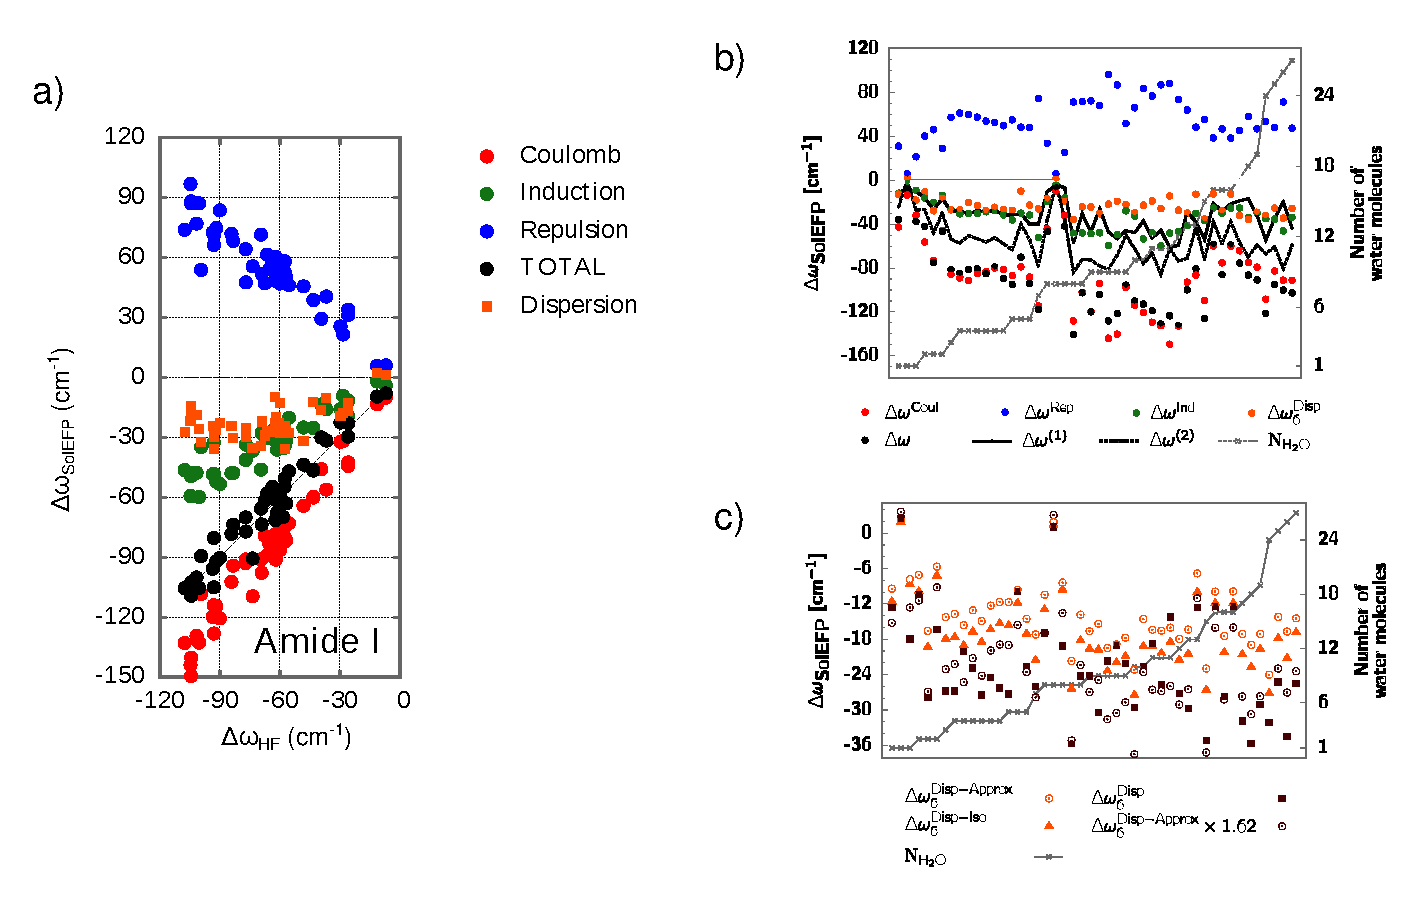
\includegraphics[width=0.97\linewidth]{NMA-water-RHF.eps}
}
\caption{
(a) The amide I mode frequency shift components that were computed
for various NMA-(H$_2$O)$_{n = 1-35}$ clusters using 
SolEFP//HF/6-311++G** method. The repulsion interaction induces amide I
frequency blueshifts, whereas the induction (distributed multipole\hyp{}induced
dipole interaction) interaction causes amide I frequency redshifts.
For the sake of comparison, we plot also dispersion frequency shifts
but they are not accounted for in `TOTAL' due to HF approximation studied here.
(b) Frequency shift decomposition as a function of the number of water molecules.
Here, the first\hyp{} and second\hyp{}order frequency shift contributions,
$\Delta\omega^{(1)}$ and $\Delta\omega^{(2)}$, are explicitly shown. It is clear
that second\hyp{}order (dispersion and induction) effects are even stronger 
that first\hyp{}order effect due to Heitler\hyp{}London solute\hyp{}solvent
interaction potential.
(c) Various levels of theoretical approximation of dispersion frequency
shifts of amide I mode that were computed for $\Delta\omega^{\rm Disp}$,
$\Delta\omega^{\rm Disp-Iso}$ and $\Delta\omega^{\rm Approx}$ 
from Eqs.~\eqref{e:dw-disp-6-distr-working}, \eqref{e:dw-disp-6-iso-distributed} 
and \eqref{e:dw-disp-6-iso-approx-distributed}, respectively.
\label{f:nma-water-rhf}}
\end{figure}
%

\paragraph{Non\hyp{}additivity of induction effects}

Before we go further and investigate electron correlation
effects, let us analyse the induction effects more closely.
It is apparent from our SolEFP theory that, except from induction, 
all the other contributions to the vibrational solvatochromism
are pair\hyp{}wise additive.\footnote{This is of course approximation
but works very well for $\Delta\omega^{\rm Coul}$ and $\Delta\omega^{\rm Ex-Rep}$
and also reasonably well for $\Delta\omega^{\rm Disp}$.} 
We have quantitatively estimated
the extent of two and three\hyp{}body effects for $\Delta\omega^{\rm Ind}$
for a model NMA--(H$_2$O)$_3$ cluster E shown in Fig.~\ref{f:nma-abcde}. 
We compare the frequency shifts computed for the whole cluster 
with the sum of frequency shifts of three
separate dimers. Here, the sets of internal coordinates of
involved molecules are deliberately set to be the same for
direct comparisons. Then, we considered the excess induction
frequency shift of NMA--(H$_2$O)$_3$
complex, which is defined as
%
\begin{equation}
\Delta\Delta\omega^{\rm Ind}(\text{ABC}) = \Delta\omega^{\rm Ind}(\text{ABC})
 - \Delta\omega^{\rm Ind}(\text{A}) - \Delta\omega^{\rm Ind}(\text{B}) - \Delta\omega^{\rm Ind}(\text{C})
\end{equation}
%
The excess frequency shift can be partitioned into two\hyp{} and three\hyp{}water components as follows 
%
\begin{equation}
\Delta\Delta\omega^{\rm Ind}(\text{ABC}) = 
\Delta^2\Delta\omega^{\rm Ind}(\text{AB}) +
\Delta^2\Delta\omega^{\rm Ind}(\text{AC}) +
\Delta^2\Delta\omega^{\rm Ind}(\text{BC}) +
\Delta^3\Delta\omega^{\rm Ind}(\text{ABC})
\end{equation}
%
with
%
\begin{subequations}
\begin{align}
\Delta^2\Delta\omega^{\rm Ind}(\text{AB}) &= 
   \Delta\omega^{\rm Ind}(\text{AB}) - 
   \Delta\omega^{\rm Ind}(\text{A})  -
   \Delta\omega^{\rm Ind}(\text{B}) \\
\Delta^3\Delta\omega^{\rm Ind}(\text{ABC})&=
   \Delta\omega^{\rm Ind}(\text{ABC}) -
\sum_\text{X} \Delta\omega^{\rm Ind}(\text{X}) -
\sum_{\text{X}<\text{Y}} \Delta^2\Delta\omega^{\rm Ind}(\text{XY})
\end{align}
\end{subequations}
%
In the above equations, $\Delta^2\Delta\omega^{\rm Ind}(\text{AB})$
and $\Delta^3\Delta\omega^{\rm Ind}(\text{ABC})$
mean the two\hyp{} and three\hyp{}water effect on the excess induction frequency shift,
respectively. These contributions are gathered in Table~\ref{t:ind-nonadd}
%
\begin{table}[t!]
\caption{
Many\hyp{}body analysis of excess polarization frequency
shift (in cm$^{-1}$) of NMA--(H$_2$O)$_3$ tetramer obtained by using 
SolEFP//HF/6-311++G** method. Water molecules occupy the H-bonding sites
A, B, and C as depicted in Fig.~\ref{f:nma-abcde}.
\label{t:ind-nonadd}}
\begin{tabular*}{1.0\textwidth}{@{\extracolsep{\fill} } l cccccc }
\hline\hline
\multicolumn{7}{c}{$\Delta\omega^{\rm Ind}$} \\
\hline
ABC     &&   AB      &&    AC     &&     BC \\
-24.08  &&   -10.24  &&   -22.08  && -11.95 \\
        &&   A       &&    B      &&     C  \\
        &&  -9.40    &&    0.34   &&  -11.13 \\
$\Delta\Delta\omega^{\rm Ind}$ && \multicolumn{3}{c}{$\Delta^2\Delta\omega^{\rm Ind}$} && $\Delta^3\Delta\omega^{\rm Ind}$ \\
\cline{1-1}
\cline{3-5}
\cline{7-7}
-3.89 && AB && -1.18 && 0.00 \\
      && AC && -1.55 &&      \\
      && BC && -1.16 &&      \\
\hline\hline
\end{tabular*}
\end{table}
%
We found that the total enhancement of the induction effect
due to the three\hyp{}body interactions (NMA--two water molecules)
constitutes 16\% of the total frequency shift whereas the four\hyp{}body
effect (NMA--three water molecules) is zero.
This clearly demonstrates that induction effect on the vibrational
frequency shift is strongly non\hyp{}additive and at least three\hyp{}body
interactions need to be properly considered in the calculations.

\subsubsection{Electron Correlation Effects}

HF approximation does not take into account the correlation
of electronic motion other than Fermi correlation
that is due to the Pauli repulsion of electrons occupying the same
molecular orbital. Let us re-investigate the same NMA--H$_2$O
and NMA--CHCl$_3$ clusters A, B, C and D that are now optimised
at MP2/6-311++G** level. The associated SolEDS frequency shifts
of the amide I mode are gathered in Table~\ref{t:mp2-soleds-amide-I}.
For the sake of comparison, we also analyse the amide II mode.
%
\begin{table}[t!]
\caption{
SolEDS (constrained cluster) frequency shifts of amide I mode computed for three NMA--H$_2$O dimers 
and NMA--CHCl$_3$ dimer by using second
order M{\o}ller-Plesset (MP2) perturbation theory and the 6-311++G** basis set. 
Full QM (MP2) harmonic
frequencies were obtained for fully optimised clusters shown in Fig.~\ref{f:nma-abcde}. 
The root\hyp{}mean\hyp{}square (RMS) of
superimposition between all atoms of constrained and fully optimised clusters is also given. The RMS between
C--C--N--C atoms of NMA is put in parentheses. See Section~\ref{s:soleds} and Eq.~\eqref{e:dw-soleds-mp2}
for the description of the frequency shift terms analysed here.
\label{t:mp2-soleds-amide-I}}
\begin{tabular*}{1.0\textwidth}{@{\extracolsep{\fill} } l ccccccccccc }
\hline\hline
 & \multicolumn{8}{c}{NMA--H$_2$O} && \multicolumn{2}{c}{NMA--CHCl$_3$} \\
\cline{2-9}
\cline{11-12}
 & \multicolumn{2}{c}{dimer A} && 
    \multicolumn{2}{c}{dimer B} && 
    \multicolumn{2}{c}{dimer C} && 
    \multicolumn{2}{c}{dimer D} \\
 & \multicolumn{2}{c}{0.06 (0.06) a.u.} && 
    \multicolumn{2}{c}{1.6 (0.1) a.u.}   && 
    \multicolumn{2}{c}{0.2 (0.04) a.u.}  && 
    \multicolumn{2}{c}{0.08 (0.01) a.u.} \\
\cline{2-12}
 & \multicolumn{11}{c}{Amide I mode} \\
\cline{2-12}
 & MEA & MEA+EA &&  MEA & MEA+EA && MEA & MEA+EA && MEA & MEA+EA \\
\hline
 $\Delta \omega_{{\rm el}}^{(10)}$      & -67.5  & -64.3   && -26.0  & -24.6   && -63.7  & -56.4  && -64.0 & -64.3 \\
 $\Delta \omega_{{\rm ex}}^{\rm HL}$    &  58.2  &  60.7   &&  13.5  &  15.7   &&  40.8  &  41.3  &&  60.1 &  65.9 \\
 $\Delta \omega_{{\rm del}}^{\rm HF}$   & -26.7  & -27.5   &&  -6.1  &  -6.6   && -21.3  & -22.8  && -26.3 & -30.7 \\
 $\Delta \omega_{{\rm el,r}}^{(12)}$    &  11.3  &  16.0   &&   3.2  &   3.6   &&   9.5  &  13.1  &&  15.1 &  17.0 \\
 $\Delta \omega_{{\rm ex}}^{(2)}$       &  11.7  &  13.1   &&   1.5  &   2.3   &&  10.5  &  11.5  &&  11.4 &  16.2 \\
 $\Delta \omega_{{\rm disp}}^{(20)}$    & -12.2  & -13.0   &&  -2.3  &  -3.0   &&  -8.5  &  -8.8  && -14.2 & -14.8 \\
 $\Delta \omega_{\rm MP2}$              & -25.2  & -15.0   &&  -16.2 & -12.6   && -32.7  & -22.0  && -17.9 & -10.7 \\
 Full QM                                &        & -17.8   &&        &  -8.4   &&        & -21.3  &&       & -15.4 \\
\hline
 & \multicolumn{11}{c}{Amide II mode} \\
\cline{2-12}
 & MEA & MEA+EA &&  MEA & MEA+EA && MEA & MEA+EA && MEA & MEA+EA \\
\hline
 $\Delta \omega_{{\rm el}}^{(10)}$      &  -6.9  & -10.2   &&  17.3  &  18.3   &&   7.2  &   5.7  &&  -4.3 &   0.1 \\
 $\Delta \omega_{{\rm ex}}^{\rm HL}$    &  30.7  &  35.4   &&  -3.0  &   6.1   &&   1.6  &   2.0  &&  30.2 &  28.9 \\
 $\Delta \omega_{{\rm del}}^{\rm HF}$   &  -5.7  &  -7.5   &&   4.4  &   2.1   &&   1.9  &   1.2  &&  -4.7 &  -3.5 \\
 $\Delta \omega_{{\rm el,r}}^{(12)}$    &  -0.6  &   0.0   &&  -2.3  &  -3.3   &&  -0.9  &   0.1  &&  -0.9 &  -1.3 \\
 $\Delta \omega_{{\rm ex}}^{(2)}$       &   5.0  &   6.4   &&   0.2  &   1.7   &&   0.45 &   0.7  &&   5.0 &   4.8 \\
 $\Delta \omega_{{\rm disp}}^{(20)}$    &  -6.7  &  -8.5   &&   0.7  &  -1.1   &&  -0.5  &  -1.0  &&  -8.2 &  -8.2 \\
 $\Delta \omega_{\rm MP2}$              &  15.8  &  15.6   &&  17.3  &  23.8   &&   9.75 &   8.7  &&  17.1 &  20.8 \\
 Full QM                                &        &  14.7   &&        &  25.3   &&        &  12.4  &&       &  11.8 \\
\hline\hline
\end{tabular*}
\end{table}
%
From the above analysis results we can see that the dispersion
interaction\hyp{}induced frequency shift is smaller than that from
the other effects at HF level. In
addition, it is confirmed that
the mechanical anharmonicity
contribution is much larger than the electric
anharmonicity contribution in all the cases
studied here except from the $\Delta \omega_{{\rm el}}^{(10)}$ contribution for amide I mode 
in dimer C and the amide II mode
$\Delta \omega_{{\rm ex}}^{\rm HL}$ values when
water molecule interacts with the amide proton
(dimer B).
In the latter exceptional case the second derivatives of exchange\hyp{}
repulsion energy with respect to the amide II normal coordinate
cannot be neglected at all. 
%This can also be seen in the similar analysis at HF level from Table~\ref{t:amide-I-soleds-solefp}.
Nevertheless, in the case of the amide I mode, the
electric anharmonicity contributions are negligible except for
the first\hyp{}order electrostatic interaction
which is relatively easy to evaluate within SolEFP model, in contrast to
other contributions.

Electron correlation manifests in the intermolecular
dispersion interaction energy and in the resulting vibrational
frequency shift of the amide I mode, though they are negligibly
small in the case of the amide II mode. Unfortunately, it is
not possible to directly compare our SolEFP solvatochromism
results with the SolEDS calculations because of the difference
in theoretical levels describing the vibrational potential energy
surface of NMA (SolEFP uses HF wavefunctions). Therefore,
we rather focus on the frequency shift derived from the HF
wavefunctions as well as that from the electron correlation
effect induced by intermolecular dispersion interaction. The
SolEDS analysis shows that the frequency shifts due to dispersion
interactions between NMA and water as well as between
NMA and chloroform are negative for the studied model
dimers and they are non\hyp{}negligible. It is especially interesting
to note that, in the case of the NMA\hyp{}CHCl$_3$ dimer, the amide
II mode frequency shift is dictated by exchange\hyp{}repulsion
interaction with negligibly small Coulomb contribution.

\paragraph{Solvatochromic dispersion coefficients\label{s:nma-sol-disp}}

Now we focus strictly on the intermolecular dispersion
interaction contribution to the vibrational frequency shifts.
Within SolEFP model, dispersion is derived from properties
at HF level by using first\hyp{}order response theory
and coupled\hyp{}perturbed Hartree\hyp{}Fock theory.
Thus, already at HF level, we can estimate the intermolecular
electron correlation effects.

We have computed the solvatochromic dispersion coefficients
$C_{j,6}$ (see Eq.~\eqref{e:cj6}) for amide I, II and A modes for the pairs NMA--X
where X is H$_2$O, methanol (MeOH), ethanol (EtOH), DMSO,
dimethylformamide (DMF), dichloromethane (CH$_2$Cl$_2$), chloroform
(CHCl$_3$), tetrachloromethane (CCl$_4$), tetrahydrofuran
(THF), benzene, and cyclohexane (Table~\ref{t:cj6}),
and compared them with the conventional $C_6$ dispersion coefficients
computed at the same level HF/6-311++G**. 
%
\begin{table}[t!]
\caption{
Isotropic solvatochromic dispersion $C_{j,6}$ coefficients of various
molecular pairs involving NMA molecule computed
by using Eq.~\eqref{e:cj6} and HF/6-311++G** method. Conventional dispersion
isotropic $C_6$ coefficients evaluated from Eq.~\eqref{e:c6} at the same level are also
shown for comparison. All values in a.u.
\label{t:cj6}}
\begin{tabular*}{1.0\textwidth}{@{\extracolsep{\fill} } l cccccccc }
\hline\hline
 && \multicolumn{5}{c}{Dispersion $C_{j,6}$} && \\
\cline{3-7}
NMA && Amide I && Amide II && Amide A && $C_6$ \\
\hline
H$_2$O       && 0.78 && 2.40  && 11.59 && 158.0 \\
MeOH         && 2.06 && 5.86  && 28.82 && 405.8 \\
EtOH         && 3.76 && 11.46 && 55.38 && 748.1 \\
DMSO         && 5.05 && 13.35 && 66.85 && 980.7 \\
DMF          && 5.74 && 17.35 && 83.98 && 1141.6 \\
CH$_2$Cl$_2$ && 3.74 && 10.00 && 49.93 && 727.2 \\
CHCl$_3$     && 4.96 && 13.17 && 65.89 && 963.6 \\
CCl$_4$      && 6.94 && 20.01 && 97.96 && 1361.5 \\
THF          && 5.92 && 17.42 && 84.84 && 1165.4 \\
Benzene      && 7.26 && 20.15 && 99.61 && 1429.6 \\
Cyclohexane  && 8.28 && 23.96 && 117.2 && 1620.1 \\
\hline\hline
\end{tabular*}
\end{table}
%
The values of $C_6$ coefficients
can
be rough indications of the relative strength of dispersion interactions
between two molecules (when all the molecules are separated by the same
distance). We found that the dispersion solvatochromic coefficients
increase with the increase of the dispersion coefficient for the interaction
energy. Moreover, the extent of increase in both coefficient series
is similar. For instance, the $C_{j,6}$ coefficient of the
amide I mode of NMA--CHCl$_3$ is about 6 times larger than
that of NMA--H$_2$O and that the $C_6$ value of NMA--CHCl$_3$ is
also about 6 times larger than that of NMA--H$_2$O. Therefore,
it is possible to conclude that the dispersion interaction
strength is generally in good correlation with the dispersion
interaction\hyp{}induced frequency shift. This is particularly important
because, when a given IR probe is in a non\hyp{}polar or aprotic
environment such as inner region of protein, the vibrational
frequency shift of the IR probe is likely to be determined
by the short\hyp{}range interactions like repulsive and dispersive
terms.

The approach based on the molecular $C_{j,6}$ coefficients 
is definitely too crude approximation and the distributed approaches
should be used for quantitative calculations. 
In Section ~\ref{s:disp} we have developed two
approximate schemes of the most accurate expression in Eq.~\eqref{e:dw-disp-6-distr-working}
representing $\Delta\omega^{\rm Disp}_6$. The simplest
one is based on the isotropic distributed coefficients $C_{j,6}^{ab}$
that are computed for the particular LMO-LMO pair, and is given
in Eq.~\eqref{e:dw-disp-6-iso-approx-distributed}. 
The second one is more involved (Eq.~\eqref{e:dw-disp-6-iso-distributed}) since
it includes terms proportional to $r^{-7}_{ab}$ but still neglects the anisotropy
of the dispersion effect. Here we tested the two approximations
and compared them with the most accurate, anisotropic dispersion
interaction\hyp{}induced frequency shifts where
the off\hyp{}diagonal dynamic polarizability tensor components
are also considered.

As can be seen from Fig.~\ref{f:nma-water-rhf}c,
$\Delta \omega_{6}^{\rm Disp-Approx}$ approximation generally
underestimates the frequency red shift roughly by a factor of 1.6,
as compared to $\Delta\omega^{\rm Disp}_6$ calculation results.
The inclusion of $r^{-7}_{ab}$\hyp{}dependent terms contribute 
only little to the shifts. Thus, the anisotropic dispersion effects
are not completely negligible for the amide I mode frequency shift
in water and they should be included. On the other hand, it is interesting
to note that, on average, all the $\Delta \omega_{6}^{\rm Disp-Approx}$
estimations can by scaled by 1.62 to reproduce the corresponding $\Delta\omega^{\rm Disp}_6$
values. This could be used as a way of fast and easy to implement
procedure of computing dispersion frequency shifts from isotropic
coefficients with including anisotropic effects by a scaling factor.
Unfortunately, such a scaling
factor is different for other solvents 
(we show later in Section.~\ref{s:amide-I-bulk} that 
$\Delta \omega_{6}^{\rm Disp-Approx}\approx\Delta \omega_{j,6}^{\rm Disp}$
in CDCl$_3$). 
Nevertheless, from the present calculations, we conclude that the dispersion
interaction between NMA and surrounding water molecules
induces an amide I frequency shift of about --30 cm$^{-1}$, which is
comparable to $\Delta \omega^{\rm Ind}$.

\subsubsection{Orientation and Distance\hyp{}Dependence of Frequency Shift Components\label{s:amide-I-orient}}

It is well known that Coulombic interactions are relatively long range forces
and can be either attractive or repulsive, depending on the orientation
of molecules.
Induction and dispersion effects are shorter\hyp{}range attractive forces but still
can be considered as moderately long\hyp{}range since they typically
extend over a few solvation shells. Exchange\hyp{}repulsion interactions
and charge\hyp{}transfer decay very fast with intermolecular distances
and they are short\hyp{}range effects, mostly extending only to the first
neighbour molecule. The first is always repulsive and the second is attractive.

Similarly, vibrational frequency shifts that originate due to the above
forces will have distinct characteristics. Let us first investigate
the simple situation when NMA interacts with one water or CHCl$_3$ molecule.
We have performed the calculations in which solvent molecule were rotated
and translated away from NMA. In Figures~\ref{f:nma-orient-a}, \ref{f:nma-orient-b}
and \ref{f:nma-orient-d}, the corresponding scans are presented.
The starting point was solute\hyp{}solvent complex in its equilibrium geometry
with $\theta=0$ and $R_d=0$, where $\theta$ is the angle of rotation of solvent
molecule (see the insets in these figures) and $R_d$ is the displacement along the H-bond axis.
Positive values of $R_d$ denote moving solvent away from solute. We have performed
the total scan on a grid of 80 translations for $R_d\in [-1.0,3.0]\text{a.u.}$ 
and 360 rotations every 1\textdegree.

We found that only $\Delta\omega^{\rm Coul}$ is a strongly directional
contribution (i.e., it contributes to blue or red shifts depending on the
relative orientation of the molecules) whereas all the remaining effects
give either blue shifts \emph{or} red shifts. Interestingly, $\Delta\omega^{\rm Disp}$
is red\hyp{}shifting when
the water molecule interacts with the NMA carbonyl oxygen,
whereas it is positive blue-shifting when water interacts with
the amide proton of NMA.

We also found that $\Delta\omega^{\rm Ex-Rep}$
decays the fastest among all the contributions to the vibrational frequency shift
and is short\hyp{}range effect, much like the conventional exchange\hyp{}repulsion interaction energy.
Induction and dispersion frequency shifts decay quite fast as well. To see the
distance\hyp{}dependencies more clearly we have computed frequency shifts
of NMA in a bulk aqueous and CHCl$_3$ solutions by taking into account
the first $N$ solvent molecules within $R_{\rm Max}$ distance between centre of
mass. They are plotted in Figs.~\ref{f:nma-water-dist} and \ref{f:nma-cdcl3-dist}. 
It is clear that $\Delta\omega^{\rm Ind}$
and $\Delta\omega^{\rm Disp}$ effects are rather long\hyp{}range
and on average 3--4 solvation shells are necessary to converge them with increasing $R_{\rm Max}$.
In contrast, $\Delta\omega^{\rm Ex-Rep}$ requires only the first and second solvation
shells and 13 Bohr cutoff is sufficient. In the above analyses we have not studied
the charge\hyp{}transfer orientation\hyp{} and distance dependencies
because it was shown to be quite negligible (c.f.
Table~\ref{t:amide-I-soleds-solefp}), at least in the case when
NMA interacts only with neutral molecules.

%
\afterpage{
\begin{figure}[t!]
\centering
\setlength\fboxsep{0.4pt}
\setlength\fboxrule{0.5pt}
\fbox{
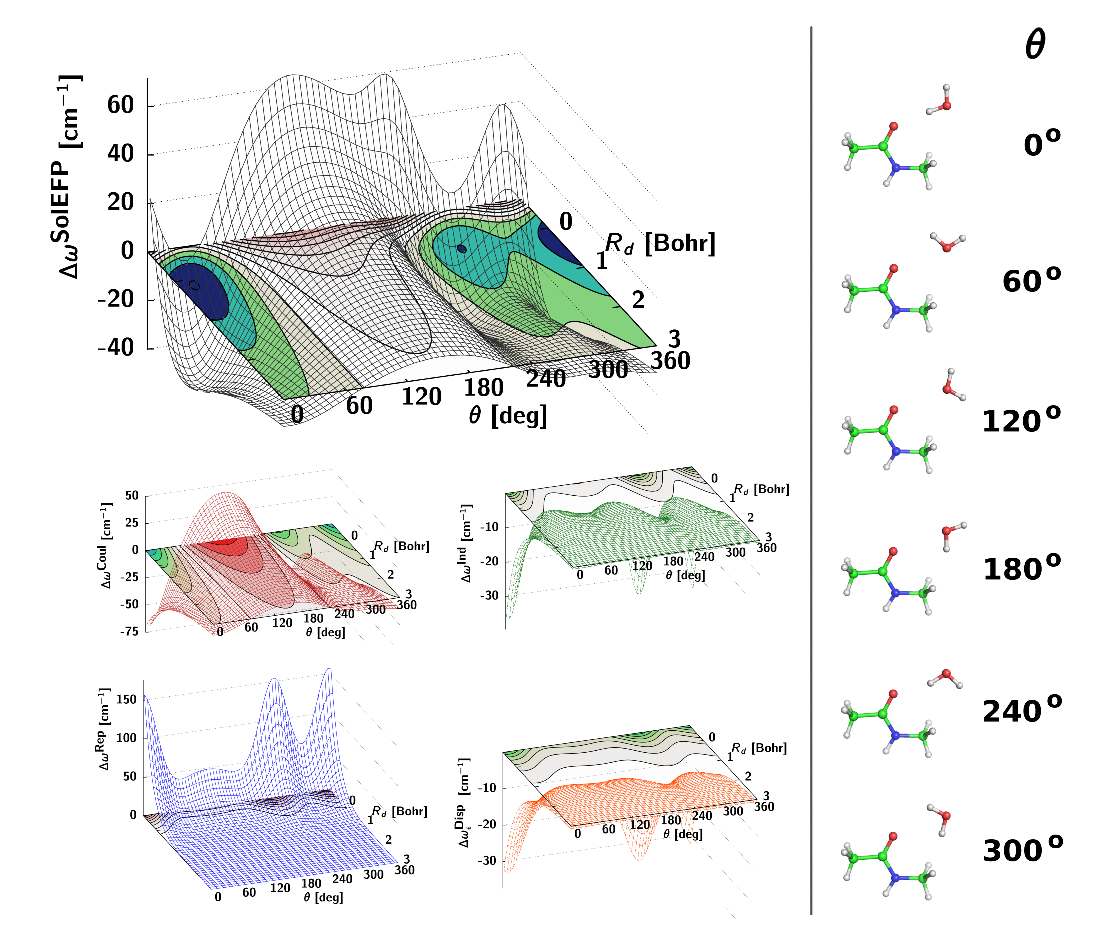
\includegraphics[width=0.97\linewidth]{NMA-orient-A.eps}
}
\caption{
Scan of amide I mode frequency shifts for NMA interacting 
with one water molecule via carbonyl oxygen atom. 
The NMA--water dimer was first optimised
by using the HF/6-311++G** method 
($R_d = 0$ and $\theta = 0$). 
The water molecule was then translated with respect to 
NMA and rotated around its centre of mass (COM) in the plane 
of NMA backbone atoms (C--C--N--C). $R_d$ stands for the translation 
distance along the direction specified by the NMA
carbonyl oxygen atom and COM of water. The orientation of the water 
molecule is also schematically depicted in the inset at the 
right\hyp{}hand side of the figure.
\label{f:nma-orient-a}}
\end{figure}
\clearpage
}

%
\afterpage{
\begin{figure}[t!]
\centering
\setlength\fboxsep{0.4pt}
\setlength\fboxrule{0.5pt}
\fbox{
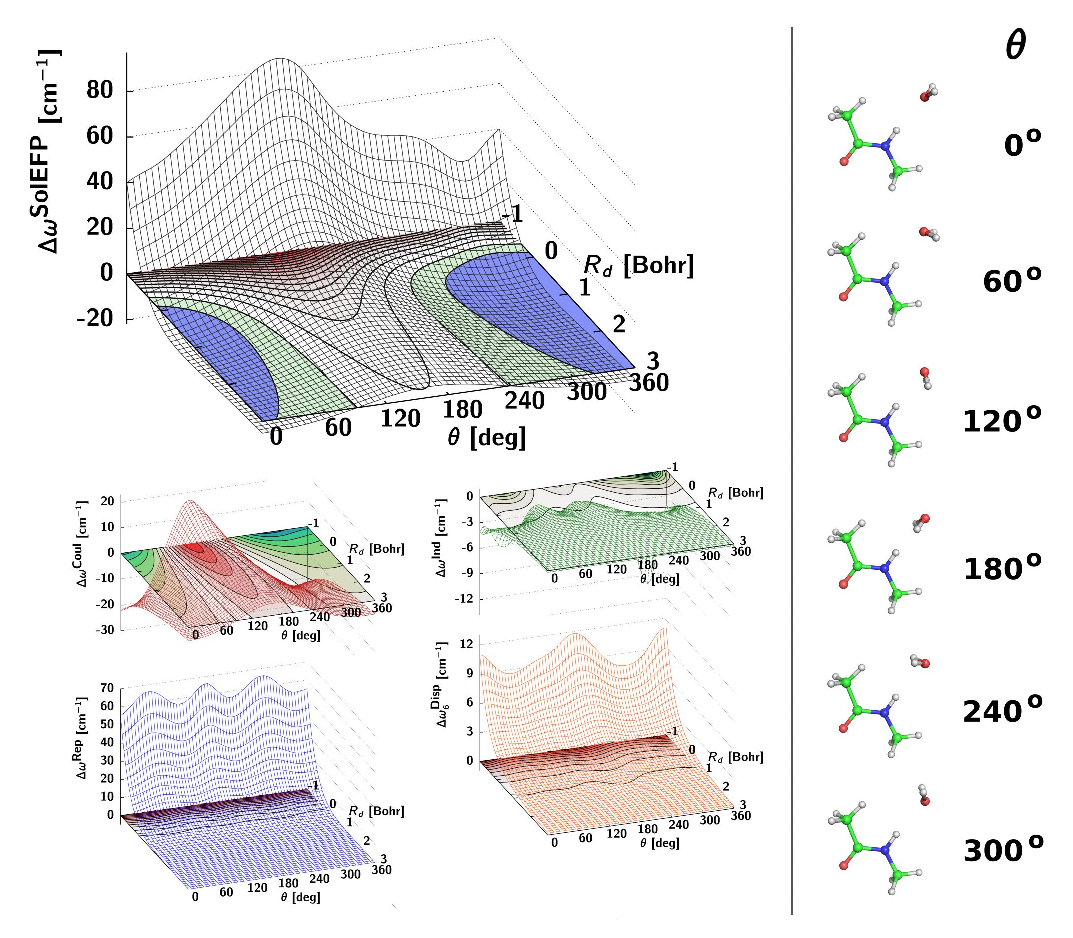
\includegraphics[width=0.97\linewidth]{NMA-orient-B.eps}
}
\caption{
Scan of amide I mode frequency shifts for NMA interacting 
with one water molecule via amide proton of NMA.
The NMA--water dimer was first optimised
by using the HF/6-311++G** method 
($R_d = 0$ and $\theta = 0$). 
The water molecule was then translated with respect to 
NMA and rotated around its centre of mass (COM) in the plane 
of NMA backbone atoms (C--C--N--C). $R_d$ stands for the translation 
distance along the direction specified by the NMA
carbonyl oxygen atom and COM of water. The orientation of the water 
molecule is also schematically depicted in the inset at the 
right\hyp{}hand side of the figure.
\label{f:nma-orient-b}}
\end{figure}
\clearpage
}
%
\afterpage{
\begin{figure}[t!]
\centering
\setlength\fboxsep{0.4pt}
\setlength\fboxrule{0.5pt}
\fbox{
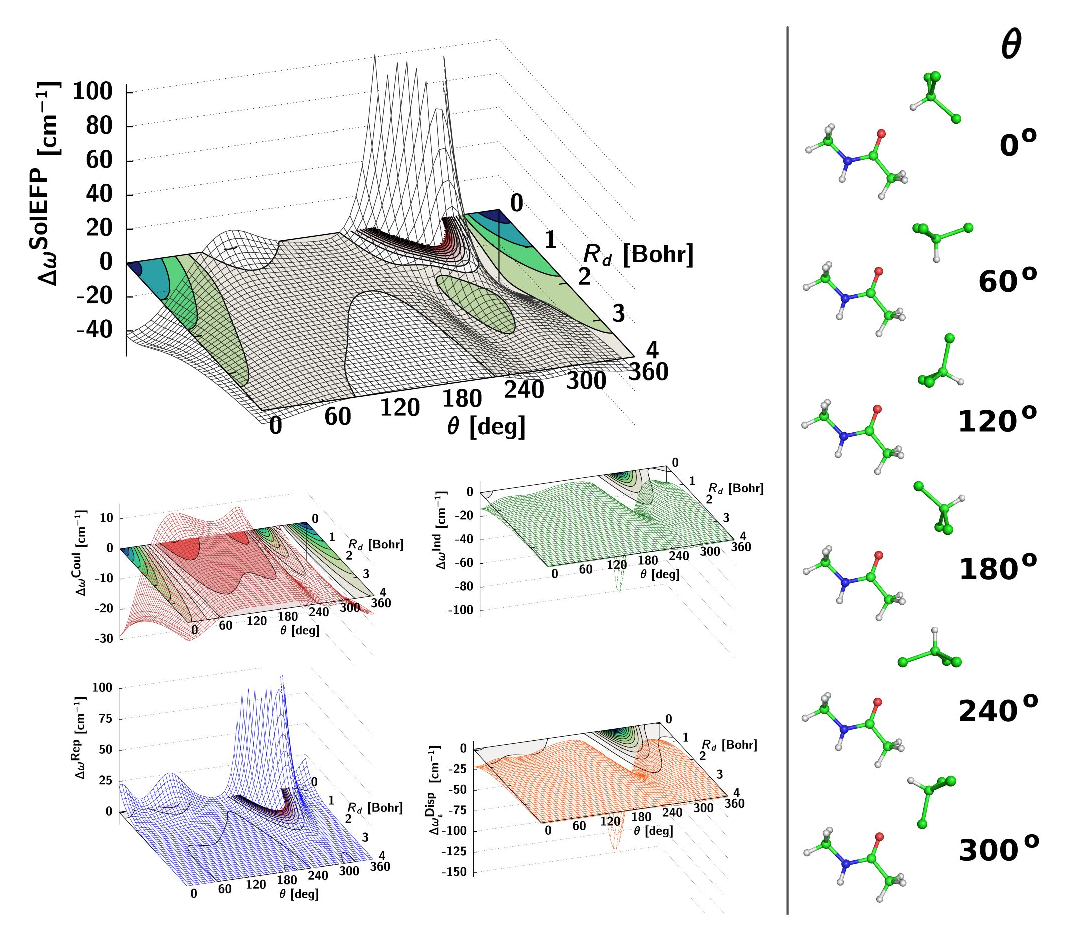
\includegraphics[width=0.97\linewidth]{NMA-orient-D.eps}
}
\caption{
Scan of amide I mode frequency shifts for NMA interacting 
with one CHCl$_3$ molecule via oxygen atom.
The NMA--CHCl$_3$ dimer was first optimised
by using the HF/6-311++G** method 
($R_d = 0$ and $\theta = 0$). 
The CHCl$_3$ molecule was then translated with respect to 
NMA and rotated around its centre of mass (COM) in the plane 
of NMA backbone atoms (C--C--N--C). $R_d$ stands for the translation 
distance along the direction specified by the NMA
carbonyl oxygen atom and COM of CHCl$_3$. The orientation of the CHCl$_3$
molecule is also schematically depicted in the inset at the 
right\hyp{}hand side of the figure.
\label{f:nma-orient-d}}
\end{figure}
\clearpage
}
%
\afterpage{
\begin{figure}[t!]
\centering
\setlength\fboxsep{0.4pt}
\setlength\fboxrule{0.5pt}
\fbox{
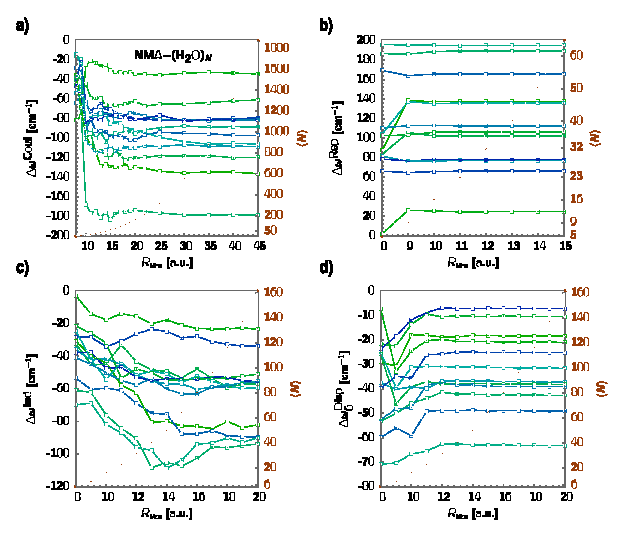
\includegraphics[width=0.97\linewidth]{cut-tip4p.eps}
}
\caption{
The convergence of the SolEFP frequency shifts with increasing $R_{\rm Max}$
for NMA in water: a) Coulomb, b) exchange\hyp{}repulsion, 
c) induction and d) dispersion frequency shifts. 
12 randomly chosen NMA--(H$_2$O)$N$ configurations from 1 ns 
NVT MD simulation at 300 K are considered. Different colours 
are used just to make it easy to distinguish results from 
different configurations sampled from MD trajectories. 
In this Figure, the numbers of water molecules averaged 
over the 12 sample configurations are also shown here 
(brown circles and line). 
\label{f:nma-water-dist}}
\end{figure}
\clearpage
}
%
\afterpage{
\begin{figure}[t!]
\centering
\setlength\fboxsep{0.4pt}
\setlength\fboxrule{0.5pt}
\fbox{
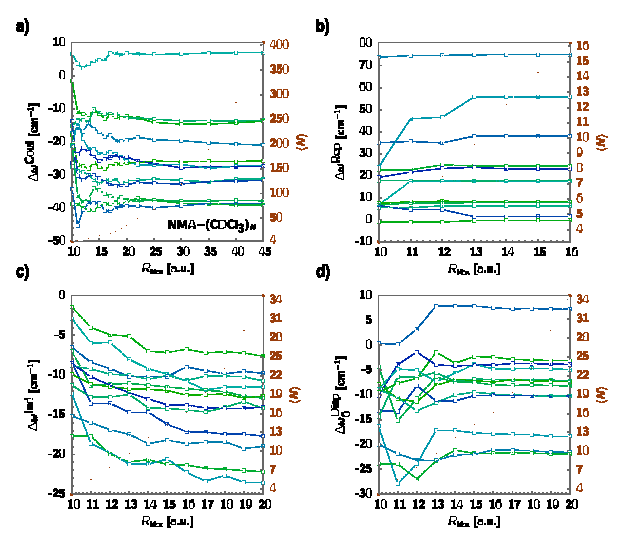
\includegraphics[width=0.97\linewidth]{cut-cdcl3.eps}
}
\caption{
The convergence of the SolEFP frequency shifts with increasing $R_{\rm Max}$
for NMA in CDCl$_3$: a) Coulomb, b) exchange\hyp{}repulsion, 
c) induction and d) dispersion frequency shifts. 
12 randomly chosen NMA--(CDCl$_3$)$N$ configurations from 1 ns 
NVT MD simulation at 300 K are considered. Different colours 
are used just to make it easy to distinguish results from 
different configurations sampled from MD trajectories. 
In this Figure, the numbers of water molecules averaged 
over the 12 sample configurations are also shown here 
(brown circles and line). 
\label{f:nma-cdcl3-dist}}
\end{figure}
\clearpage
}
%





\section{Modelling Vibrational Solvatochromism in Bulk\label{s:amide-I-bulk}}

In order to model real systems it is desirable to consider
models of bulk solutions rather than small solute\hyp{}solvent
clusters. We have performed CMD simulations of NMA (in \emph{trans}
conformation) in water and CDCl$_3$ and we have applied the rigid
molecule algorithm for SolEFP to the resulting CMD trajectories 
(see Chapter 8 for the detailed
discussion and implementation), and the results are gathered
in Table~\ref{t:amide-I-bulk}.
%
\afterpage{
\begin{table}[t!]
\caption{
Experimental vibrational frequencies of the amide I mode of
NMA in gas phase, H$_2$O and CDCl$_3$, and frequency shifts relative to gas
phase state obtained by SolEFP/6-311++G**//Parm99 method. In this
Table, we also show full width at half maximum (FWHM) of vibrational
frequency shift static distributions obtained from SolEFP//Parm99 calculations.
All values in cm$^{-1}$.
\label{t:amide-I-bulk}}
\begin{tabular*}{1.0\textwidth}{@{\extracolsep{\fill} } l ccccc }
\hline\hline
\multirow{5}{*}{Gas phase} & 1731$^a$ & \multirow{5}{*}{$\Delta\omega^{\rm Expt.}$} 
                                      & \multirow{5}{*}{$\Delta\omega^{\rm SolEFP//Parm99}$} 
                                      & \multirow{5}{*}{Error} & \\
                           & 1714$^a$ & &&&\\
                           & 1731$^b$ & &&&\\
                           & 1713$^b$ & &&&\\
                           & 1728$^c$ & &&&\\
\hline
\multirow{3}{*}{H$_2$O}    & 1619$^d$ & \multirow{3}{*}{-100 $\pm$8} 
                                      & \multirow{3}{*}{-95.1$\pm$3} 
                                      & \multirow{3}{*}{+4.9} & \\
                           & 1625$^a$ & &&&\\
                           & 1628$^e$ & &&&\\
CDCl$_3$                   & 1669$\pm$3$^f$ & -55$\pm$6 & -39.1$\pm$3 & +15.9 &\\
%
\hline\hline
        &  \multicolumn{5}{c}{Static distribution} \\
\cline{2-6}
Solvent & $\Gamma^{\rm Coul}$ & $\Gamma^{\rm Ex-Rep}$ & $\Gamma^{\rm Ind}$ & $\Gamma^{\rm Disp}_6$ & $\Gamma^{\rm SolEFP}$ \\
\hline
H$_2$O  &     62 $\pm$ 3      &    112 $\pm$ 10       &     47 $\pm$ 4     &    34 $\pm$ 2         &       69 $\pm$ 3      \\
CDCl$_3$&     37 $\pm$ 3      &     25 $\pm$ 5        &      9 $\pm$ 1     &    22 $\pm$ 2         &       51 $\pm$ 3      \\
\hline\hline
\end{tabular*}
\begin{footnotesize}
$^a$Ref. \citep{Kubelka.Keiderling.JPCA.2001}; 
$^b$Ref. \citep{LumleyJones.JMolSpectrosc.1963}; 
$^c$Ref. \citep{Mayne.Hudson.JPC.1991}; 
$^d$Ref. \citep{Chen.Schweitzer-Stenner.Asher.Mirkin.Krimm.JPC.1995}; 
$^e$Ref. \citep{Eaton.Symons.Rastogi.JChemSocFaradayTrans1.1989}; 
$^f$Ref. \citep{DeCamp.DeFlores.McCracken.Tokmakoff.Kwac.Cho.JPCB.2005}.
\end{footnotesize}
\end{table}
}
%

First of all, the SolEFP model combined with classical
MD simulation reproduces the amide~I mode frequency
shift by water solvation almost perfectly (deviation is about
+5~cm$^{-1}$), whereas the difference (+16~cm$^{-1}$) between our
SolEFP and experimentally measured amide I frequency shifts
in chloroform solution is a bit larger than that in water.
However, it should be emphasised that the SolEFP equations
presented and used in this work do not contain any empirical
parameters nor rely on fitting and that the vibrational responses
of the amide~I modes to solvation are fully derived from the
first\hyp{}principles theory based on the gas\hyp{}phase (not solution phase)
molecular properties. Here, the only empirical aspect
in our theory is in the CMD force field parameters that determine
the ensemble of solute\hyp{}solvent configurations.

The approximation of $\Delta\omega^{\rm Disp}_6$
based on the distributed
solvatochromic dispersion parameters ($\Delta\omega^{\rm Disp-Approx}_6$)
works
well in CDCl$_3$ solution, but it is not sufficiently accurate for
water -- note that it counts just 56\% of $\Delta\omega^{\rm Disp}_6$
(Figure~\ref{f:nma-solefp-md}).
%
\begin{figure}[t!]
\centering
\setlength\fboxsep{0.4pt}
\setlength\fboxrule{0.5pt}
\fbox{
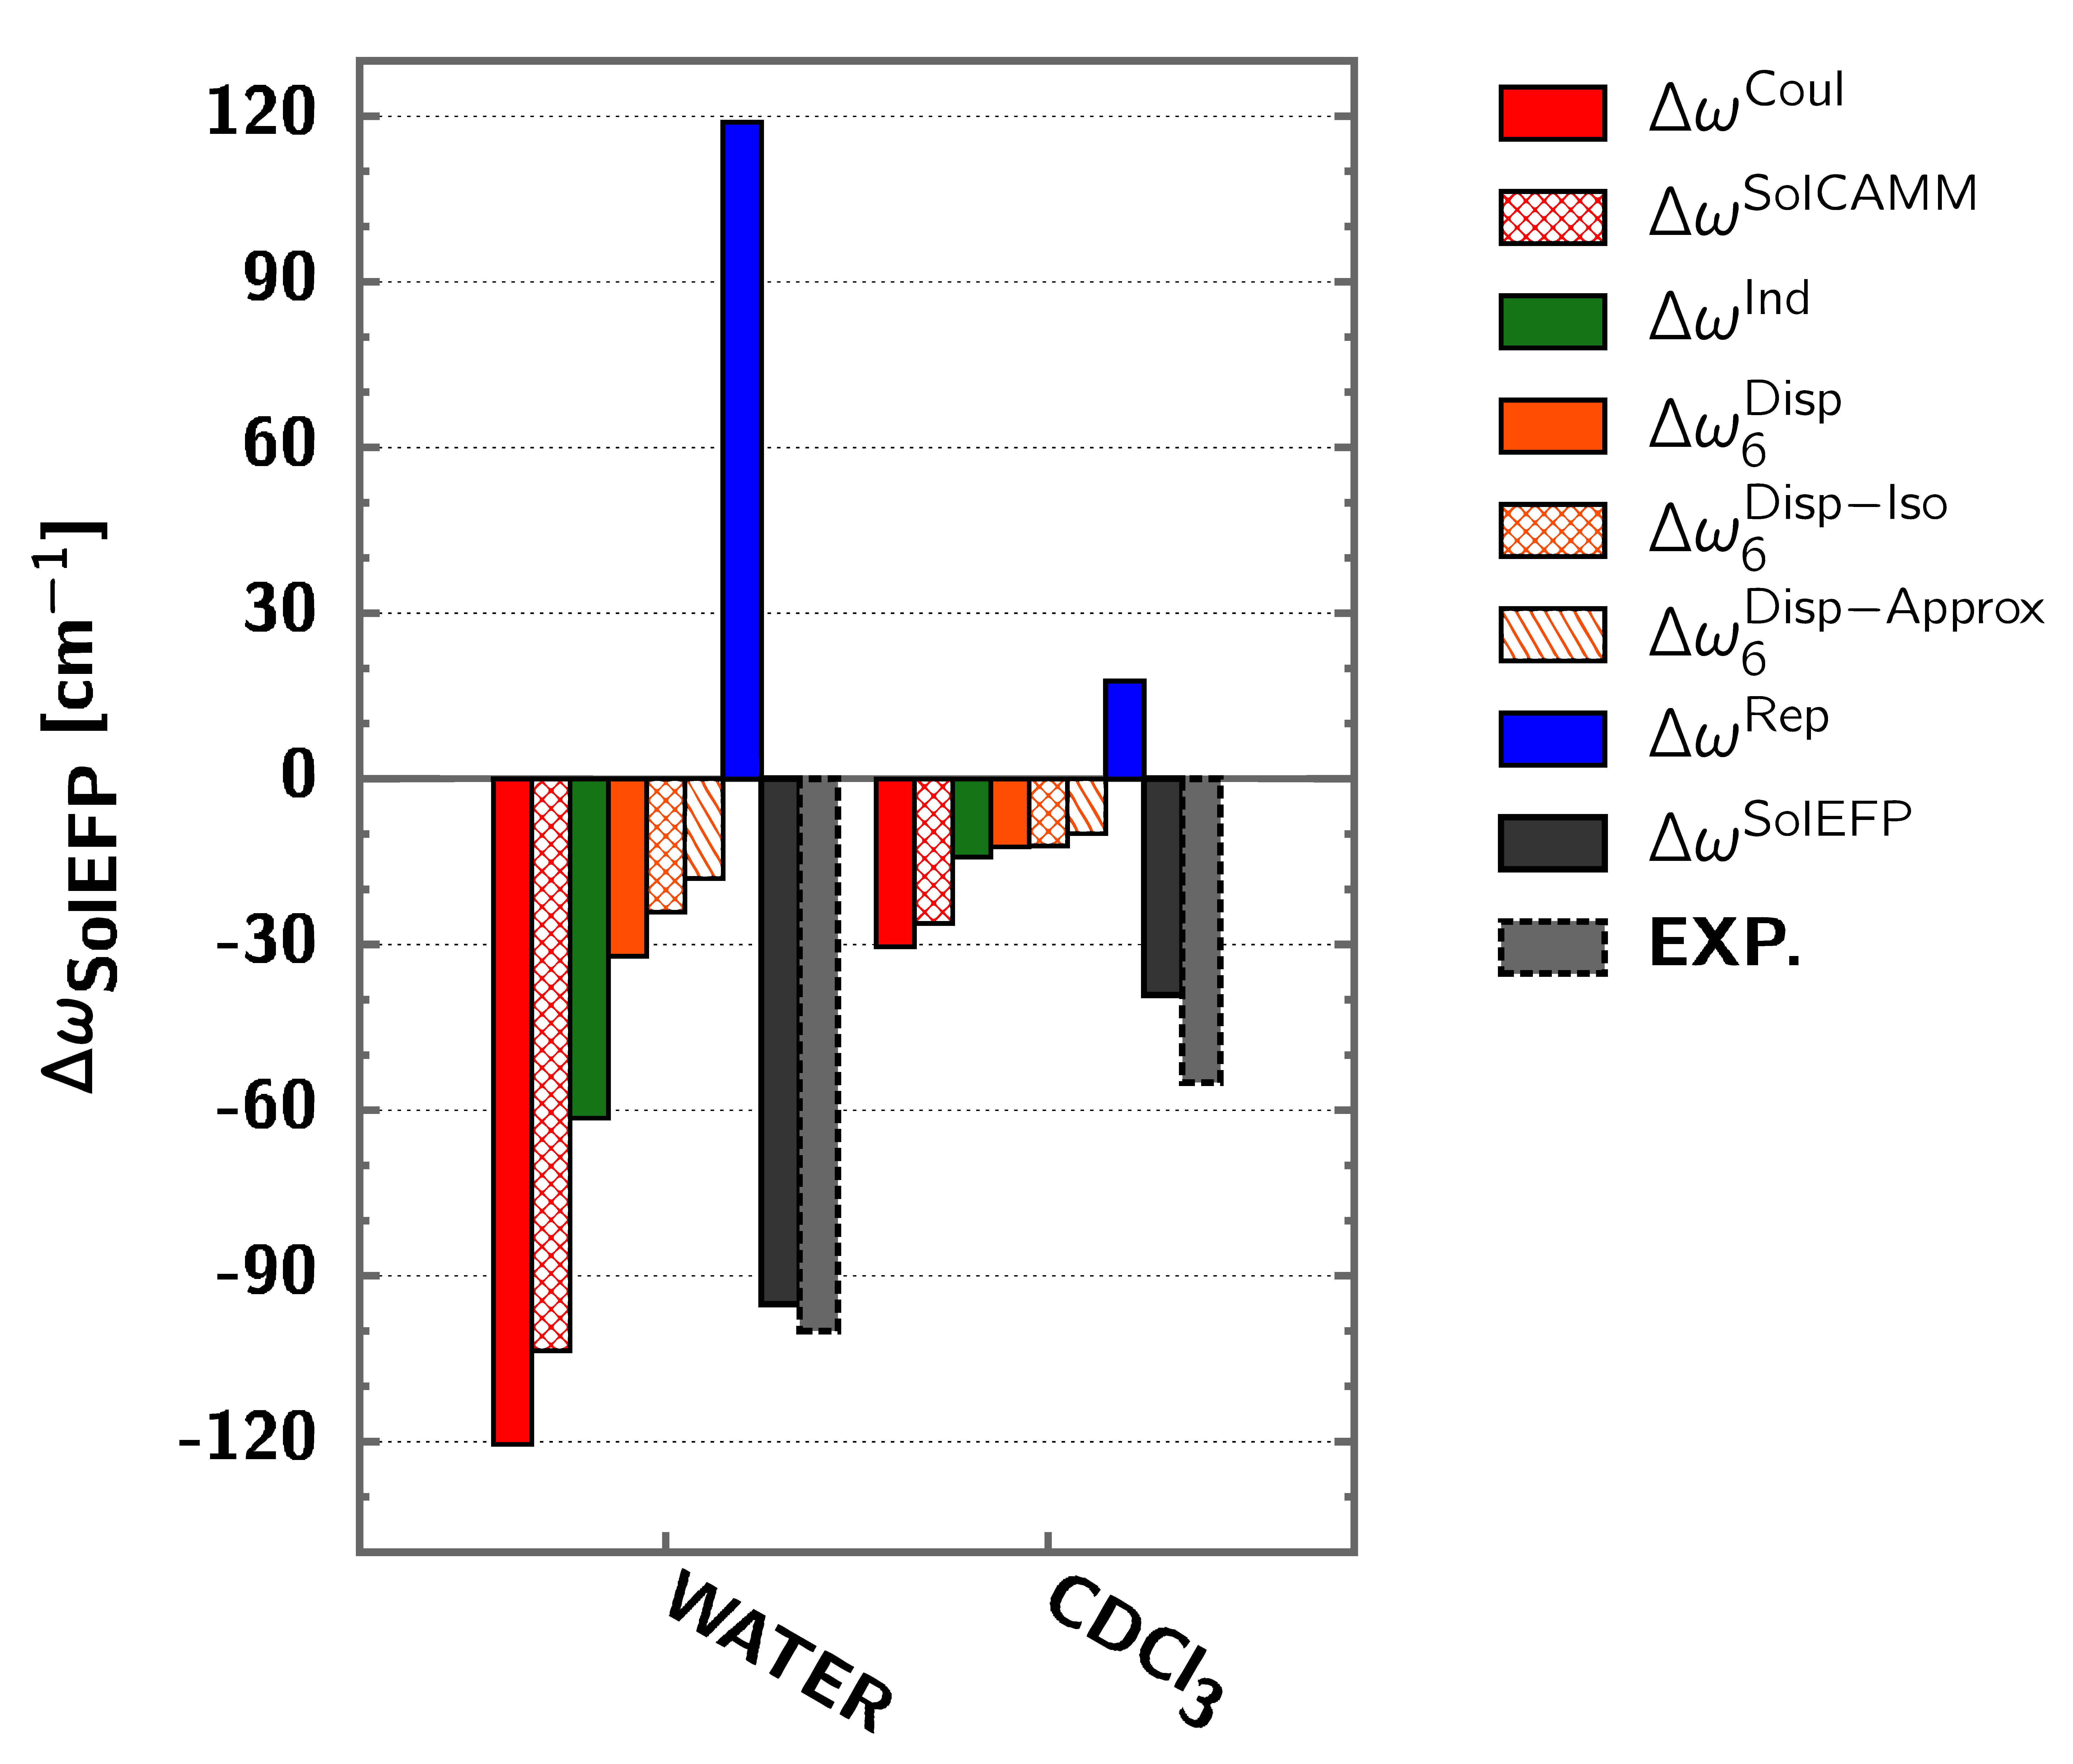
\includegraphics[width=0.9\linewidth]{NMA-water-cdcl3-SolEFP.eps}
}
\caption{
Origins of frequency shifts of the NMA amide~I mode 
in H$_2$O and CDCl$_3$ analysed by applying 
the SolEFP theory to molecular dynamics trajectories. 
Experimental frequency shifts are also shown for comparison.
\label{f:nma-solefp-md}}
\end{figure}
%
However, applying the scaling factor 1.62 derived from the
procedure in Section~\ref{s:nma-sol-disp} 
gives the value of --29~cm$^{-1}$, which
is quite close to the correct value of --32~cm$^{-1}$. This means
that the scaling factor could be derived from a small set of
solute\hyp{}solvent clusters just in the case that the computationally
easy scheme of evaluating $\Delta\omega^{\rm Disp-Approx}_6$ is preferred over the very
complicated expression for $\Delta\omega^{\rm Disp}_6$.

To carefully examine the contributions from the four
different contributions to the vibrational frequency shifts, 
we plot the frequency shift distributions
separately in Figures~\ref{f:nma-solefp-md-distr}a and 
\ref{f:nma-solefp-md-distr}b for NMA/water and
NMA/chloroform solutions, respectively. 
%
\begin{figure}[t!]
\centering
\setlength\fboxsep{0.4pt}
\setlength\fboxrule{0.5pt}
\fbox{
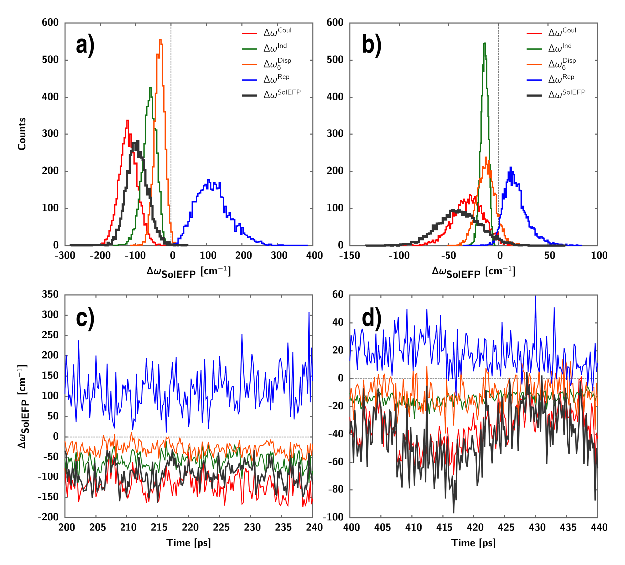
\includegraphics[width=0.9\linewidth]{NMA-SolEFP.MD-distr.eps}
}
\caption{
Amide I mode frequency shift distributions and instantaneous 
frequency shift trajectories obtained by combining 
the SolEFP//HF/6-311++G** method with molecular dynamics 
simulation. Panels (a) and (c): NMA in H$_2$O; panels (b) and (d): 
NMA in CDCl$_3$. In panels (b) and (d), selected 40 ps fragments 
of frequency shift trajectories were depicted.
\label{f:nma-solefp-md-distr}}
\end{figure}
%
In water, the peak
frequency of the $\Delta\omega^{\rm Coul}$ distribution is further red\hyp{}shifted by
-20~cm$^{-1}$ with respect to $\Delta\omega^{\rm SolEFP}$, but the shape of $\Delta\omega^{\rm Coul}$
distribution is almost identical to that of $\Delta\omega^{\rm SolEFP}$ distribution.
On the other hand, in CDCl$_3$, the $\Delta\omega^{\rm SolEFP}$ distribution appears
to be much broader than the $\Delta\omega^{\rm Coul}$ distribution mainly due
to the short\hyp{}range dispersion and exchange\hyp{}repulsion effects.
This means that, in chloroform, the amide I frequency shift
results from delicate balances among the Coulomb, induction,
dispersion, and exchange\hyp{}repulsion effects. Note also that,
while the $\Delta\omega^{\rm Ind}$ distribution in CDCl$_3$ is very narrow, the
corresponding distribution in H$_2$O is much broader, which
indicates that NMA specifically interacts with water molecules
also via induction interaction.



\section{Discussion}

\subsection{Origins of Vibrational Solvatochromism\label{s:amide-I-discuss-origins}}

Unlike the previous attempts to describe vibrational
frequency shifts of amide I mode in polar solvents with the
Coulomb interaction terms only, it is now clear that the nature
of the vibrational solvatochromism of the amide I mode in
solutions is rather complicated. Nevertheless, the first\hyp{}order
electrostatic interaction\hyp{}induced effects still dominate the
frequency shift (see the black and red lines in Figures~\ref{f:nma-solefp-md-distr}c 
and \ref{f:nma-solefp-md-distr}d). 
In particular, we found that the dispersion interaction\hyp{}induced
term contributes about 30\% to the total SolEFP
frequency shifts. Nonetheless, it is still not clear why our
estimated $\Delta\omega^{\rm SolEFP}$ value of the amide I frequency of NMA in
chloroform deviates from the experimental value by as much
as +16~cm$^{-1}$. Probably, this can be resulted from the inaccuracy
of force field parameters for chloroform. Indeed, Jansen \citep{Jansen.JPCB.2014}
showed that a careful tuning of the force field parameters
for chlorine atoms of chloroform significantly improves the
accuracy of his electrostatic map. They further showed that
the higher\hyp{}order multipole moments of chlorine atoms and
induction interactions are important for realistically simulating
the NMA/chloroform solution.

With the SolEFP model, it becomes possible to understand
why the purely electrostatic models reported here and
previously by others work very well for predicting the amide
I frequency shift in water. In Figures~\ref{f:nma-orient-a}, 
\ref{f:nma-orient-b} and \ref{f:nma-orient-d} we showed that only the Coulomb
contribution, $\Delta\omega^{\rm Coul}$, changes its sign when a polar solvent
molecule changes its relative orientation with respect to the
NMA while keeping the solute\hyp{}solvent distance fixed. In
addition, it is clear
that $\Delta\omega^{\rm Coul}$ is the largest contribution when the intermolecular
distance is not too short. Consequently, $\Delta\omega^{\rm Coul}$ dominates the
amide I vibrational frequency shift. Furthermore, it is noted
that water molecule is very small, has large dipole moment
(roughly 1.8 D), and has fewer electrons than CDCl$_3$. Thus,
it has spatially localised charge distribution so that it can
strongly interact with vibrational solvatochromic multipole
moments of the amide I mode of NMA. This leads to
a large Coulombic vibrational interaction. It was in fact
noticed previously by Jansen and Knoester \citep{Jansen.Knoester.JCP.2006} 
that, in the case
of DMSO-$d_6$ solvent, their semi\hyp{}empirical electrostatic map
works quantitatively well (within the errors of 7 cm$^{-1}$ for
the peak position and 3 cm$^{-1}$ for the FWHM), despite that
DMSO is a comparatively large and polarizable molecule.
This agreement can now be attributed to its large dipole
moment (about 4.0 D) that makes the electrostatic interaction
the dominant factor for the amide I frequency shift in DMSO.
In contrast, even though CDCl$_3$ also is still much larger
than water, it has a small dipole moment ($\sim$1 D) so that
all the other (non\hyp{}Coulombic) terms contribute to the amide
I frequency shift equally importantly. Note that, if the van
der Waals interaction effects are taken into account in the
vibrational map as Ma{\l}olepsza and Straub \citep{Malolepsza.Straub.JPCB.2014} did, the line
shape becomes comparable to the experimentally measured
spectrum, though their map was partly obtained by fitting to
the experimental data. Although we have not provided the
simulated line shapes of the IR absorption spectra here, our
FWHM values of the $\Delta\omega^{\rm Coul}$ and $\Delta\omega^{\rm SolEFP}$ frequency shift
distributions ($\Gamma^{\rm Coul}$ and $\Gamma^{\rm SolEFP}$) in chloroform solution are 37
and 51 cm$^{-1}$, respectively. This is, respectively, 1.9 and 2.7
times larger than the electrostatic calculation of Jansen and
Knoester ($\sim$19 cm$^{-1}$) for NMA-$d$. \citep{Jansen.Knoester.JCP.2006,Jansen.JPCB.2014} 
In contrast, our $\Gamma^{\rm Coul}$
in water (62 cm$^{-1}$) is almost the same as their prediction
in D$_2$O ($\sim$60 cm$^{-1}$). \citep{Jansen.Knoester.JCP.2006} 
This supports our hypothesis that the
non\hyp{}Coulombic solvatochromic effects are more pronounced
in chloroform than in water, which could affect the modelling
of the line shape, though our $\Gamma^{\rm Coul}$ value in CDCl$_3$ is about 2
times larger than that of the calculation of Jansen~\emph{et al.}

Recently, Farag~\emph{et al.} \citep{Farag.Ruiz-Lopez.Bastida.Monard.Ingrosso.JPCB.2015} 
showed that the effect of intermolecular
interaction potential on the vibrational frequency
shifts of the NMA amide I mode in water is negligible, in
stark disagreement with previous findings. \citep{Blasiak.Lee.Cho.JCP.2013,Blasiak.Cho.JCP.2014} 
They concluded that the frequency shifts are the
direct manifestation of the structural distortion due to solvation,
separating those effects from intermolecular interaction.
However, one should be careful when interpreting the results,
because there is a notable difference between their definition
of interaction energy components and the meaning of $U$ in our
SolEFP or SolEDS theories. In the approach of Farag~\emph{et al.},
the interaction energy between solute and solvent molecules
was described as follows:
%
\begin{equation} \label{e:farag}
 U =  E^{\rm es} + E^{\rm pol} + E^{\rm CT} + E^{\rm def}
\end{equation}
%
where the corresponding interaction terms, originating from
the divide\hyp{}and\hyp{}conquer interaction energy decomposition
scheme, \citep{vanderVaart.Merz.JPCA.1999} 
stand for the ``electrostatic'', ``polarization'', ``charge\hyp{}transfer''
and ``structural deformation'', respectively. It is
important to underline here that the ``electrostatic'' component
in Eq.~\eqref{e:farag} actually includes the exchange\hyp{}overlap contribution
as well, similarly to the remaining terms. \citep{vanderVaart.Merz.JPCA.1999} 
Note also that the
structural deformation term is separated from others in their
approach, which is not the case in our approach. 
It should be noted that, in the work of Farag~\emph{et al.}, 
all of these four terms were evaluated for the relaxed
NMA--water complex and the change in vibrational frequency
is elucidated based on the vibrational potential energy surface
of the amide I mode after NMA relaxes to a new geometry (due
to its interaction with water) -- note that the NMA in that case
is not the same with the isolated NMA in the gas phase. In their
case, the solvatochromic interaction\hyp{}induced property is not
directly related to isolated molecular properties, because most
of the associated effects by solvation are already included in
the structural deformation term, $E^{\rm def}$. In contrast, in the coarse\hyp{}grained
models of the vibrational solvatochromism \citep{Buckingham.ProcRSocLondonA.1958,
Buckingham.ProcRSocLondonA.1960,
Buckingham.TransFaradaySoc.1960,
Cho.JCP.2003,Cho.JCP.2009} 
that are
the theoretical foundation of SolEFP and SolEDS models, the
solvation\hyp{}induced vibrational frequency shift is related to the
gas\hyp{}phase geometrical change of the solute due to solvation.
In fact, the WCA frequency shift can be rewritten in
the following form:
%
\begin{equation} \label{e:pstro}
\Delta\omega_j = \frac{1}{2M_j\omega_j} \left\{
  \sum_i g_{ijj} \delta Q_i + \sderiv{U}{Q_j}
\right\}
\end{equation}
%
where $\delta Q_i$ is the structural distortion of the $i$th normal
coordinate given by
%
\begin{equation} \label{e:cooo}
 \delta Q_i = -\frac{1}{M_i\omega_i^2} \fderiv{U}{Q_i} 
            = \delta Q_i^{\rm Coul} +
              \delta Q_i^{\rm Ex-Rep} +
              \delta Q_i^{\rm Ind} +
              \delta Q_i^{\rm Disp} +
              \delta Q_i^{\rm CT}
\end{equation}
%
In the above relation, one can directly notice the link between
$\delta Q_i$ and mechanical anharmonicity of the $j$th vibrational mode,
which means that the structural deformations’
effects were naturally included in our solvatochromism
model.\footnote{The coarse\hyp{}grained models of solvatochromism 
refer to gas\hyp{}phase state and structural distortions are deduced 
from Eq.~\eqref{e:cooo}. Therefore, there is a certain problem associated with 
the difference between EFP (gas\hyp{}phase) structures and the solvated 
solute molecule (SolEFP model). However, those differences are generally 
very small and a proper superimposition is sufficient.} 
It is thus evident from Eq.~\eqref{e:cooo} that, upon solvation,
the structural deformation affects all of the interaction energy
components. Moreover, we have shown that the mechanical
anharmonicity term is the dominant contribution to $\Delta\omega$; hence,
$\delta Q_i$ is indeed responsible for the vibrational frequency shifts.
The decomposition done by Farag~\emph{et al.} is believed to be
a confirmation of this statement so that it should be in agreement with our previous
calculations. 
We present the more detailed numerical
comparisons of our theory and the model of Farag~\emph{et al.} in
Table~\ref{t:farag}.
%
\begin{table}[t!]
\caption{
The comparison of SolEDS and Farag~\emph{et al.}'s 
model \citep{Farag.Ruiz-Lopez.Bastida.Monard.Ingrosso.JPCB.2015} 
of frequency shift partitioning. In this Table, `MA' and `EA' denote
the mechanical and electric anharmonicities, respectively,
and their sum is labelled as `TOT'.
The structures of NMA--water dimers B and C are shown in
Figure~\ref{f:nma-abcde}. All values are in cm$^{-1}$.
\label{t:farag}}
\begin{tabular*}{1.0\textwidth}{@{\extracolsep{\fill} } lccccccccc}
\hline\hline
\multicolumn{4}{c}{SolEFP model}       && \multicolumn{5}{c}{Farag~\emph{et al.}'s model} \\
\hline
\multicolumn{4}{c}{HF/6-311++G**}      && \multicolumn{5}{c}{PM3} \\
   \multicolumn{4}{c}{$\omega_{\text{Amide I}}=1908\text{ cm}^{-1}$}      
&& \multicolumn{5}{c}{$\omega_{\text{Amide I}}=1928.7\text{ cm}^{-1}$} \\
%
\hline
%
\multicolumn{4}{c}{NMA--water dimer C} && \multicolumn{5}{c}{NMA--water ``Complex 1''} \\
\cline{1-4} \cline{6-10}
 & MA & EA & TOT && $\Delta\nu_{\rm ele}^{rel}$ & $\Delta\nu_{\rm pol}^{rel}$ & $\Delta\nu_{\rm CT}^{rel}$ & $\Delta\nu_{\rm def}^{rel}$ &
                       $\Delta\nu^{rel}$ \\
\cline{2-4} \cline{6-10}
 $\Delta\omega^{\rm HF}_{\rm del}$  
          & -21.8 &  7.3  & -14.5 && \multirow{3}{*}{  7.5} &
                                     \multirow{3}{*}{ -0.8} &
                                     \multirow{3}{*}{ -3.0} &
                                     \multirow{3}{*}{-29.3} &
                                     \multirow{3}{*}{-25.7} \\ 
 $\Delta\omega^{\rm HF}_{\rm del}$    
          & -11.9 & -1.5  & -13.4 && & & & &       \\
 $\Delta\omega^{\rm SolEDS}$    
          & -33.7 &  5.8  & -27.9 && & & & &       \\
 Full QM  &      &        & -28.4 && & & & & -26.0 \\
%
\hline
%
\multicolumn{4}{c}{NMA--water dimer B} && \multicolumn{5}{c}{NMA--water ``Complex 3''} \\
\cline{1-4} \cline{6-10}
 & MA & EA & TOT && $\Delta\nu_{\rm ele}^{rel}$ & $\Delta\nu_{\rm pol}^{rel}$ & $\Delta\nu_{\rm CT}^{rel}$ & $\Delta\nu_{\rm def}^{rel}$ &
                       $\Delta\nu^{rel}$ \\
\cline{2-4} \cline{6-10}
 $\Delta\omega^{(10)}_{\rm el}+\Delta\omega^{\rm HL}_{\rm ex}$ 
          & -10.8 &  3.2  &  -7.6 && \multirow{3}{*}{  1.0} &
                                     \multirow{3}{*}{  0.1} &
                                     \multirow{3}{*}{  0.0} &
                                     \multirow{3}{*}{ -9.3} &
                                     \multirow{3}{*}{ -8.2} \\ 
 $\Delta\omega^{\rm HF}_{\rm del}$    
          &  -3.4 & -0.4  &  -3.8 && & & & &       \\
 $\Delta\omega^{\rm SolEDS}$    
          & -14.2 &  2.8  & -11.4 && & & & &       \\
 Full QM  &       &       & -11.4 && & & & & -26.0 \\
%
\hline\hline
\end{tabular*}
\end{table}
%
Here, we compare the frequency shifts of the amide~I modes for two different 
NMA--water dimers that were specifically investigated by us and by Farag~\emph{et al.} 
``Complex 1'' and ``Complex 3'' in the work of Farag~\emph{et al.} 
(see Figure 4 and Table 4 in Ref.~\citep{Farag.Ruiz-Lopez.Bastida.Monard.Ingrosso.JPCB.2015}) 
corresponds to the dimers ``C'' and ``B'' 
in our paper, respectively. Despite that the complexes were treated 
with different methods (PM3 vs HF/6-311++G**), the overall frequency shifting 
patterns should be comparable. 

The frequency shift of the amide~I mode, according to Farag~\emph{et al.}, is divided into
%
\begin{equation} \label{e:cooo2}
 \Delta\nu^{rel} =  \Delta\nu_{\rm ele}^{rel} +
                    \Delta\nu_{\rm pol}^{rel} +
                    \Delta\nu_{\rm CT}^{rel} +
                    \Delta\nu_{\rm def}^{rel}
\end{equation}
%
In order to compare the above partitioning terms with our SolEDS calculations, we have
changed the definition of $\Delta\nu_{\rm ele}^{rel}$, $\Delta\nu_{\rm ele}^{pol}$,
$\Delta\nu_{\rm ele}^{CT}$ and $\Delta\nu_{\rm ele}^{def}$ with respect to their 
original definition (by a multiplying factor of 2; see Eq.(7) 
in Ref.~\citep{Farag.Ruiz-Lopez.Bastida.Monard.Ingrosso.JPCB.2015}). 
It is evident that the deformation term in Farag~\emph{et al.}'s 
refers to our mechanical anharmonic contribution in the SolEDS analysis.
Moreover, $\Delta\nu_{\rm ele}^{rel}$ term corresponds to the sum of the 
first\hyp{}order electrostatic and exchange\hyp{}repulsion frequency shifts 
within the electronic anharmonicity approximation. This is because 
``electrostatic'' contribution in the interaction energy decomposition 
scheme of van der Vaart~\emph{et al.} \citep{vanderVaart.Merz.JPCA.1999}  
includes the antisymmetrization of wavefunction 
already -- note that it solves local self\hyp{}consistent\hyp{}field (SCF) 
problems for each molecule by computing global Fock matrix 
(thus it could be approximately associated with the Heitler\hyp{}London term). 
Therefore, Farag~\emph{et al.}'s partitioning into
``electrostatics'', ``polarization'' and ``charge\hyp{}transfer” terms
describes, to a large extent, only (minor) electric anharmonicity
effects! (To see this, refer to Eq.~\eqref{e:pstro}.) This is
why the interaction induced frequency shifts in their model
are negligible as compared to ``deformation'' contribution.
In particular, the ``electrostatic'' shift in the model of Farag~\emph{et al.}
refers to the sum of the Coulombic and exchange\hyp{}repulsion
electric anharmonicity terms, i.e., Heitler\hyp{}London
term. For example, in the case of the NMA--water complex ``C''
(Figure~\ref{f:nma-abcde} and Table~\ref{t:amide-I-soleds-solefp}), 
SolEDS//HF/6-311++G** calculations predict
this sum to be +7.3~cm$^{-1}$, whereas mechanical and total
anharmonicity red shifts equal to --33.7 and --27.9~cm$^{-1}$,
respectively. The analysis made by Farag~\emph{et al.} on a similar
cluster under PM3 approximation \citep{Stewart.JCC.1988} 
gives +7.5 cm$^{-1}$ ``electrostatic''
shift and --29.3~and --26.0~cm$^{-1}$ for the mechanical and
total anharmonicity red shifts, respectively. Furthermore, the
polarization and charge\hyp{}transfer contributions considered by
Farag~\emph{et al.} are also similarly related to our model. 

Quite recently, 
Brinzer~\emph{et al.}
used CO$_2$ asymmetric
stretch ($\nu_3$) mode as an IR probe for sensing the local molecular
environments in ionic liquids and carried out two\hyp{}dimensional
IR spectroscopic studies of the local structural fluctuation dynamics
around CO$_2$ molecules in a few different ionic 
liquids. \citep{Brinzer.Berquist.Zhe.Dutta.Johnson.Krisher.Lambrecht.Garrett-Roe.JCP.2015} 
They also performed quantum chemistry vibrational analyses
of model clusters consisting of one CO$_2$ and one cation-anion
pair. It was shown that the frequency shift originating from
geometric distortion of CO$_2$ by its interaction with surrounding
ions is the dominant contribution. Furthermore, the geometric
distortion was found to be correlated with the charge transfer
effect between CO$_2$ and ions. In fact, our SolEFP theory
showed that the geometric distortion effect, which is included
in the mechanical anharmonicity term
is significantly larger than the electric anharmonicity term.
We found that the charge transfer effects on the vibrational
frequency shifts of not only the amide I mode of NMA
in water \citep{Blasiak.Cho.JCP.2014} but also the nitrile, thiocyanate, and
azide stretch modes in aqueous solutions \citep{Lee.Choi.Cho.PCCP.2010} 
were comparatively
weak. Nevertheless, it will be of great interest to further
investigate such charge transfer and other quantum mechanical
effects on the general vibrational solvatochromism of various
IR probes interacting with ionic species in solutions in the
future.

\subsection{On the Applicability of Onsager Model}

Before we close this Chapter, let us come back for a while to
continuum models since there is still some group of researchers
using it in the vibrational solvatochromism. 

It is well known that the Onsager field theory describes
the solvation phenomena of polar species surprisingly
well provided that the solvent molecules do not interact
specifically with the solute molecule, which suggests that the
solute\hyp{}solvent interaction is primarily electrostatic. This led
to believe that the vibrational frequency shift is also related
to the dipole moment change of the solute in a polar
environment. In fact, Boxer and co\hyp{}workers found that the
frequency shifts of CN stretch modes of ethyl thiocyanate
(EtSCN) \citep{Fafarman.Sigala.Herschlag.Boxer.JACS.2010} 
and some aromatic nitriles \citep{Levinson.Fried.Boxer.JPCB.2012} 
are linearly proportional
to the strength of Onsager reaction field in aprotic polar
solvents. However, it was also found that there is a considerable
disagreement with the Onsager theory for the cases
when solute molecules are non-polar or the permanent dipole
moment is approximately perpendicular to the vibrational
solvatochromic dipole \citep{Levinson.Fried.Boxer.JPCB.2012} 
or, even more interestingly, when
the solvent is protic, e.g., water and 
trifluoroethanol. \citep{Fafarman.Sigala.Herschlag.Boxer.JACS.2010}  
In the latter cases, the IR probe molecules interact with solvent
molecules via hydrogen bonds -- note that such hydrogen bonding
interaction is highly localised and substantially
increase anisotropy of electrostatic potential around the vibrational
probe of interest. This makes the simple Onsager
dipolar field theory inapplicable in such situations and considering
solvent molecules explicitly is \hyp{inevitable}. It is shown also in our 
calculations: note that the frequency shift of amide~I mode of NMA in water
is at most 30~cm$^{-1}$ whereas the experimental value
is around 100~cm$^{-1}$. We shall return to discussion
on the aspect of Onsager model and Stark spectroscopy in Chapter 5 
where we directly show that Stark\hyp{}dipole
theory fails in protic environments and is also not accurate in aprotic solvents.

\section{Summary}

In this Chapter, we have shown that the purely electrostatic
models based solely on the interaction between
solvatochromic multipoles of a solute molecule and electric
potential (or electric field) produced by partial charges of
surrounding solvent molecules are not enough to describe the
overall solvatochromic frequency shift. This will be of great
importance when one is interested in using various IR probes
to monitor local structural changes in environments where the
short\hyp{}range interaction\hyp{}induced terms, such as repulsion and
dispersion interactions, are not negligibly small.
We also showed that Onsager model of vibrational solvatochromism
should be treated as a qualitative tool in analysing vibrational
frequency shifts of amide I mode in aprotic, weakly polar solvents.

\printbibliography[heading=subbibintoc,title={References}]
\end{refsection}

% ------------------- CHAPTER 6 ------------------------

\begin{refsection}

\chapter{Vibrational Solvatochromism of CN Modes\label{c:cn-modes}}

While amide I mode can be used as a sensor of the global conformation
of proteins, isolated nitrile (CN) or azide (N$_3$) 
stretch modes can be useful IR probes for sensing the local molecular environment
around them. The chemical nature of CONH and triple bonded groups
is different. In particular, recently proposed isonitrile (NC) 
IR probe exhibits substantial sensitivity towards H-bonding.
Here we study in detail the physical origins
of the vibrational frequency shifts of CN and NC modes
in various molecular environments -- ranging from bulk solutions
to highly heterogeneous protein interiors and interfaces.
We believe that the present work could provide a set of clues 
that could be potentially used to design a rigorous
theoretical model linking vibrational solvatochromism 
and molecular topology in complex heterogeneous environments.

\section{Overview}

In the previous Chapter we were surprised by the fact that the remarkably strong
contributions to the vibrational frequency shifts by exchange\hyp{}repulsion,
induction and dispersion do not blur the directionality of the (strong)
Coulombic effects within the medium and large solute\hyp{}solvent separation ranges. 
This makes electrostatic maps generally successful for 
reproducing experimental amide I mode vibrational frequency shifts
in most types of environments. However, as we pointed out in Chapter~\ref{c:vibr-solv}, 
the solvatochromism of CN
stretch vibration in various solvents is quite complicated and
cannot be explained simply by the Coulombic interaction of
vibrational dipole with local electric field produced by
surrounding molecules, \citep{Ben-Amotz.Lee.Cho.List.JCP.1992,
Rey.Hynes.JCP.1998,
Reimers.Hall.JACS.1999,Fafarman.Sigala.Herschlag.Boxer.JACS.2010,
Morales.Thompson.JPCB.2011,
Wilderen.Luuk.Kern-Michler.Muller-Werkmeister.Bredenbeck.PCCP.2014}
%
which is in notable contrast to the
solvatochromism of CO stretch modes. \citep{Fried.Boxer.AccChemRes.2015,
Lee.Choi.Cho.JCP.2012,Fried.Bagchi.Boxer.JACS.2013}
%
By the analysis
of the forces computed from the classical molecular dynamics
simulations and their effects on the vibrational frequency, it
was found that the vibrational frequency blue\hyp{}shifts of CN
stretches of acetonitrile or CN$^-$ anion in water result from van
der Waals interactions. \citep{Rey.Hynes.JCP.1998,Morales.Thompson.JPCB.2011}
Boxer group experimentally showed that the non\hyp{}specific electrostatic and specific H-bonding
effects contribute differently to the vibrational shifts
by combining IR and NMR methods. \citep{Fafarman.Sigala.Herschlag.Boxer.JACS.2010,
Bagchi.Fried.Boxer.JACS.2012}
% 
Recently, Zhang~\emph{et al.}~\citep{Zhang.Markiewicz.Doerksen.Smith.Gai.PCCP.2015} 
studied
the specific and nonspecific nitrile frequency shifts in analogs
of 5-cyanotryptophan by utilising empirically determined
Kamlet\hyp{}Taft parameters \citep{Kamlet.Taft.JACS.1976,Taft.Kamlet.JACS.1976,
Kamlet.Abboud.Taft.JACS.1977}
%
of various solvents. They found a
simple three\hyp{}parameter linear formula that can be used to
relate the CN absorption frequency with the solvent polarity
and H-bonding properties. However, this and other similar
approaches \citep{Reimers.Hall.JACS.1999} 
are based on the empirical data and, therefore,
cannot provide detailed insights into the physical origins of the
vibrational frequency shifts. Nevertheless, it is apparent that
H-bonding interaction between nitrile and protic solvent exerts
a blue\hyp{}shift of nitrile stretch frequency, which is probably
beyond Coulomb interaction effect. 

SolEFP and SolEDS models are
perfectly suited to study these issues. As model 
IR probes, we study methyl thiocyanate and methyl\hyp{} 
or phenyl\hyp{}substituted (iso)nitriles.
We showed in Figure~\ref{f.MeCN.MeSCN.vs.solvents} 
that the vibrational solvatochromism of MeSCN is
quantitatively similar to that of MeCN. In addition, 
MeSCN probe is theoretically more convenient to study
because, unlike in MeCN case \citep{Suzuki.Nakagawa.Fujiyama.SCActaA.1977}, 
its CN stretch band is not
contaminated by other Fermi resonance bands.

First, we investigate
the vibrational solvatochromic properties of isolated
MeSCN. Next, relatively small model systems
involving hydrogen bonds are considered. The direct
comparisons with experimental results are also made for the bulk
solutions when SolEFP method is combined with QM/MM forcefield. 
The nature of the specific
solvatochromic frequency shifts of nitrile probes in proteins
are discussed further. At the end of this Chapter we compare
the CN and NC vibrational probes and explain the consequences of the 
interchange of N and C atoms, mainly the increase of the sensitivity
of the vibrational NC frequency
towards H-bonding and absorption intensity increase of NC stretch mode.

\section{Electrostatic Vibrational Properties of CN Stretch Modes}

The vibrational
solvatochromic multipole moments up to octupoles for the model
nitrile stretch modes in MeSCN were calculated by using
SolCAMM technique (for SolMMM of MeCN and MeNC see
Table~\ref{t:cnnc-solcamm} on page~\pageref{t:cnnc-solcamm}). 
In Table~\ref{t:mescn-solcamm}, the
vibrational solvatochromic (molecular not distributed) dipoles
and quadrupoles calculated with a few different
methods are directly compared. 
%
\begin{table}[t!]
\caption{
Vibrational solvatochromic dipole and traceless quadrupole moments
(at the mid\hyp{}point of CN bond) of MeSCN that were obtained with our SolMMM
method. Solvatochromic dipole and quadrupole moments are given in 
cm$^{-1}$/(MV/cm) and 10$^{-8}\times$ cm$^{-1}$/(MV/cm$^2$), respectively.
The fitting results in this table were obtained by carrying out
multivariate least square fitting analyses of HF and density functional theory
(B3LYP) calculations of MeSCN--water clusters.
\label{t:mescn-solcamm}}
\begin{tabular*}{1.0\textwidth}{@{\extracolsep{\fill} } l ccc}
\hline\hline
\multicolumn{2}{c}{Method}  & $\mu_{\rm CN}$ & $\Theta_{\rm CN}$$^{e)}$  \\
\hline
\multirow{4}{*}{SolMMM/6-311++G**}   & HF             & 0.47 & 1.16 \\
                                     & MP2            & 0.20 & 0.96 \\
                                     & CCSD           & 0.31 & 1.06 \\
                                     & B3LYP          & 0.43 & 1.26 \\
\hline
\multirow{2}{*}{Fitting}             & HF$^{a)}$      & 0.54 &      \\
                                     & B3LYP$^{b)}$   & 0.43 & 1.02 \\
\hline
Exp.$^{c)}$                          &                & 0.55--0.64$^{d)}$   & - \\
\hline\hline
\end{tabular*}
%
\begin{footnotesize}
$^{a)}$ Ref.~\citep{Choi.Oh.Lee.Lee.Cho.JCP.2008}, 
$^{b)}$ Ref.~\citep{Lee.Choi.Cho.JCP.2012}, 
$^{c)}$ Ref.~\citep{Suydam.Boxer.Biochem.2003}, 
$^{d)}$ Local field correction factor is assumed to be in
the range of 1.1--1.3, 
$^{e)}$ The average value of the traceless quadrupole was
estimated from the formula: 
$\sqrt{Q_{zz}^2 + \frac{4}{3}(Q_{xy}^2+Q_{xz}^2+Q_{yz}^2) + \frac{1}{3}(Q_{xx}-Q_{yy})^2}$.
Note that in
Ref.~\citep{Lee.Choi.Cho.JCP.2012} and Ref.~\citep{Blasiak.Lee.Cho.JCP.2013} 
the traceless quadrupole is defined according to Jackson \citep{Jackson.ClassicalElectrodynamics.1998}
whereas we use Buckingham's convention here \citep{Buckingham.QRevChemSoc.1959} 
(to convert value of
traceless quadrupole element $Q_{ij}$ from Jackson's to Buckingham's
convention multiply it by $\frac{1}{2}$).
\end{footnotesize}
\end{table}
%

Our \emph{ab initio} calculated values
of the Stark dipole of the CN stretch mode in MeSCN are in the range
from 0.2 to 0.5 cm$^{-1}$/(MV/cm), which is close to the
experimental value of MeSCN in 2-methyltetrahydrofuran
glass at 74~K (0.55--0.64 au). \citep{Suydam.Boxer.Biochem.2003} 
Evidently, our MP2 estimation
somewhat underestimates the value of the Stark dipole (0.2
cm$^{-1}$/(MV/cm)) and method treating the electron correlation
more accurately is needed (CCSD gives the result 0.31
cm$^{-1}$/(MV/cm), closer to the experimental value). This might be
also a result of too small basis set used for such calculations
but we did not extend it beyond 6-311++G** because of the
resource limitations. Nevertheless, except for MP2 results,
SolCAMM/6-311++G** method predicts the Stark tuning
rate well. In Table~\ref{t:mescn-solcamm}, for the sake of comparison we also
present the Stark tuning rates estimated by using the
distributed vibrational solvatochromic charges that were
obtained from multivariate least square fitting analyses of the
HF and DFT (density functional theory) calculation results from
a number of MeSCN--water clusters. They are in good
agreement with the experimental value. Nevertheless, it
should be emphasised that the present SolCAMM calculation
results for the (molecular not distributed) vibrational
solvatochromic dipole and quadrupole moments are fully
derived from the first\hyp{}principles without using any empirical or
fitting procedure.

%
\begin{figure}[t!]
\centering
\setlength\fboxsep{0.4pt}
\setlength\fboxrule{0.5pt}
\fbox{
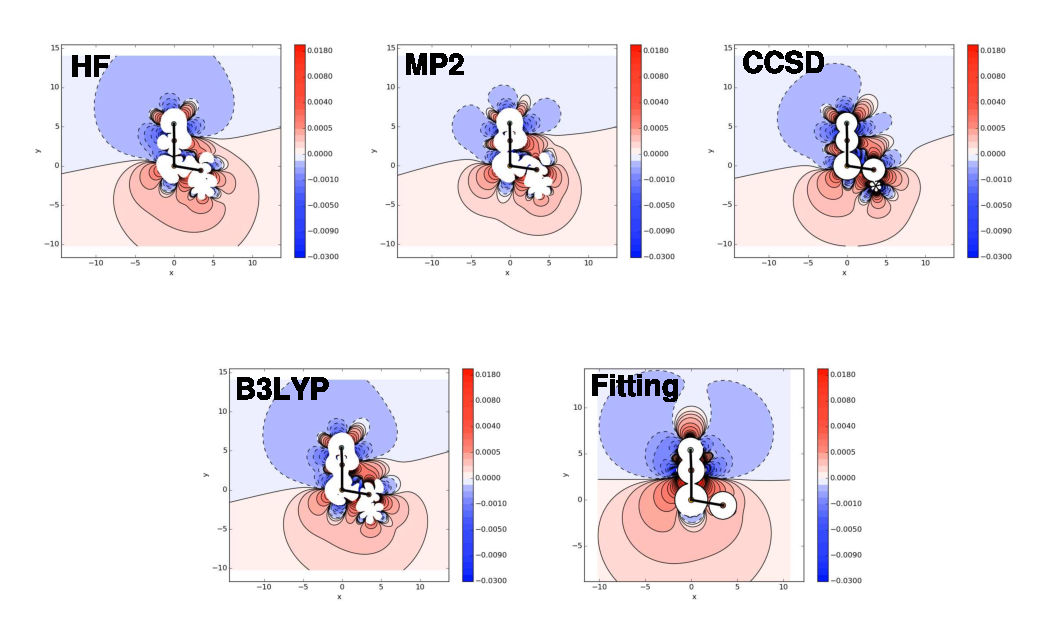
\includegraphics[width=0.9\linewidth]{mescn-solcamm-all.eps}
}
\caption{
Electrostatic potential produced by the vibrational solvatochromic multipole moments of the vibrational 0-1
transition of nitrile (CN) stretch mode in MeSCN, that were computed by using 
SolCAMM//6-311++G** method with HF, MP2, CCSD and B3LYP methods. For comparison
we also plot electrostatic potential produced by solvatochromic charges 
from Ref.~\citep{Lee.Choi.Cho.JCP.2012} (labelled as ``Fitting'' in this Figure).
\label{f:mescn-maps-all}}
\end{figure}
%
%
\begin{figure}[t!]
\centering
\setlength\fboxsep{0.4pt}
\setlength\fboxrule{0.5pt}
\fbox{
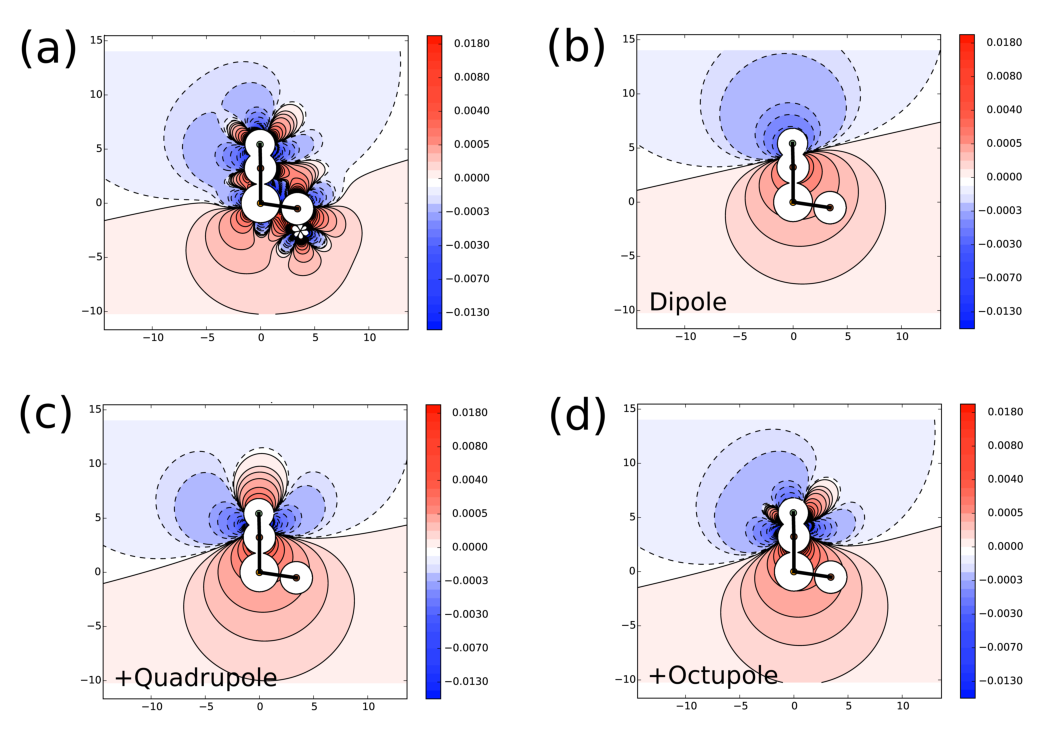
\includegraphics[width=0.9\linewidth]{Fig.2.eps}
}
\caption{
Electrostatic potential produced by the vibrational solvatochromic multipole moments of the vibrational 0-1
transition of nitrile (CN) stretch mode in MeSCN, that were computed by using 
SolCAMM//CCSD/6-311++G** method. (a) potential derived from SolCAMM (up to octupoles) distributed over all 
atoms; (b), (c) and (d) potential derived from the total molecular multipole moments (SolMMM) centred at the middle
of CN bond.
\label{f:mescn-maps}}
\end{figure}
%
In Figure~\ref{f:mescn-maps-all}, the spatial distribution of the electric
potential produced by the vibrational solvatochromic
multipole moments is plotted. Clearly, the distribution of this
electric potential around MeSCN differs from that of the
vibrational solvatochromic dipole (compare also Figures~\ref{f:mescn-maps}(a)
and \ref{f:mescn-maps}(b)), but it does not depend qualitatively
on the choice of QM method.\footnote{Note however
that the solvatochromic dipole moment
computed from least\hyp{}squares fitting procedure
is fully collinear with C$\equiv$N bond axis
because the fitting did not take into account the
methyl group. \citep{Lee.Choi.Cho.JCP.2012}} 
%
Interestingly, if
the vibrational solvatochromic quadrupole contribution is
additionally taken into account (Figure~\ref{f:mescn-maps}(c)), the corresponding
electric potential around the H-bond accepting N-atom of the
nitrile changes its sign (compare Figures~\ref{f:mescn-maps}(b) with~\ref{f:mescn-maps}(c)). Note
that this important change in the distribution of electric
potential produced by the vibrational solvatochromic
multipoles cannot be described by the Stark dipole theory at
all. Thus, even within the approximation that the vibrational
solvatochromic frequency shift solely results from the
interactions of the vibrational solvatochromic multipoles of
the solute molecule with the electric field produced by the
atomic charges of surrounding solvent molecules, the simple
dipolar description of the complicated vibrational
solvatochromism is not acceptable.

\section{H-bonding Effect on Nitrile Frequency Shift}

Although the H-bonding interaction\hyp{}induced frequency shifts
of various nitrile stretches in protic solvents have been
observed, an all\hyp{}encompassing theory for such phenomena has
not been developed yet. To theoretically study such H-bonding
effects on the nitrile frequency shift, we considered sixty seven
MeSCN--water clusters that were fully optimised at HF/6-311++G** 
level of theory. For the sake of comparisons, we
also considered fifteen MeSCN--DMSO clusters, where DMSO is
not a protic solvent molecule. The SolEFP\hyp{}calculated frequency
shifts are then directly compared with the full HF/6-311++G**
harmonic analysis results. Our SolEFP results are found to be in
good agreement with the benchmark HF/6-311++G** results,
despite the approximate nature of the SolEFP theory (see
Section~\ref{s:solefp-working-model}).

%
\begin{figure}[t!]
\centering
\setlength\fboxsep{0.4pt}
\setlength\fboxrule{0.5pt}
\fbox{
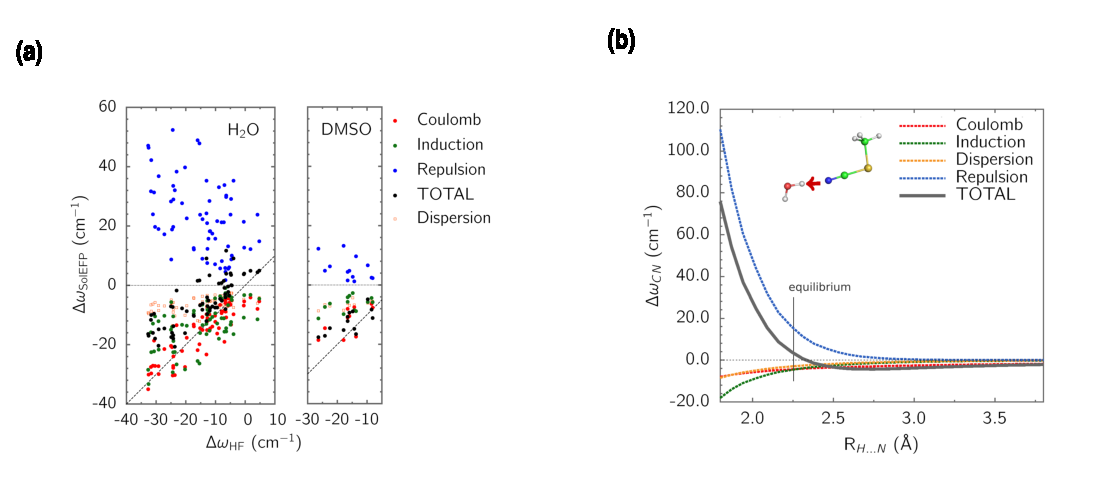
\includegraphics[width=0.9\linewidth]{Fig.3.eps}
}
\caption{
SolEFP//HF/6-311++G** frequency shift components. (a) The SolEFP components contributing to the CN
frequency shifts of MeSCN in various water and DMSO clusters, MeSCN--(H$_2$O)$_{n=1-27}$ 
and MeSCN--(DMSO)$_{n=1-7}$.
The total SolEFP frequency shifts (without dispersion) 
are also directly compared with the results from HF/6-311++G**
calculations. (b) The SolEFP components for MeSCN--water dimer with varying intermolecular distance are
plotted with respect to the distance between H(water) and N(MeSCN) atoms. The optimum H-bond distance
is at 2.2536~\AA.
\label{f:mescn-solefp-qm}}
\end{figure}
%
Our SolEFP calculation results (Figure~\ref{f:mescn-solefp-qm}(a)) show that the
exchange\hyp{}repulsion contribution (blue dots) to the nitrile
frequency shift is in general very large. In fact, the $\Delta\omega^{\rm Ex-Rep}$
contributions are almost comparable to or even larger than
the Coulomb (red dot) and induction (green dot) contributions.
To further examine the intermolecular distance dependencies
of each contribution, we calculated them separately for
varying H-bond distance between nitrile's N atom and water
H-atom (see Figure~\ref{f:mescn-solefp-qm}(b)). What is surprising to us is that the
exchange repulsion contribution, $\Delta\omega^{\rm Ex-Rep}$, is the largest among
all the other contributions in the distance range around the
equilibrium (optimum) H-bond distance ($\sim$2.25~\AA). The
electrostatic contribution, which is the sum of the Coulomb
and induction terms, is rather constant in the distance range
from 2.0 to 2.5~\AA. To examine both the distance- and
orientation\hyp{}dependence of the vibrational frequency shift
induced by its interaction with a water molecule, we carried
out further SolEFP calculations at the level of HF/6-311++G**
(Figure~\ref{f:mescn-scan}). 
%
\begin{figure}[t!]
\centering
\setlength\fboxsep{0.4pt}
\setlength\fboxrule{0.5pt}
\fbox{
\includegraphics[width=0.9\linewidth]{Fig.4.eps}
}
\caption{
Distance- and orientation\hyp{}dependence of CN stretch mode frequency shift of MeSCN interacting with water
molecule. Frequency shifts were calculated by using SolEFP method. Water molecule was translated in the
direction along the line between N and O atoms by a distance $R_d$. Water molecule was then rotated in a
plane of SCN--O atoms around its centre of mass by angle $\theta$. The structure at $R_d=0$ and $\theta=0$ corresponds to
the equilibrium (optimal H-bonding) geometry of MeSCN-H$_2$O dimer, which was obtained with
HF/6-311++G** method.
\label{f:mescn-scan}}
\end{figure}
%
%\afterpage{
\begin{figure}[t!]
\centering
\setlength\fboxsep{0.4pt}
\setlength\fboxrule{0.5pt}
\fbox{
\includegraphics[width=0.98\linewidth]{Fig.S2-5.scaled.eps}
}
\caption{
Cutoff distance\hyp{}dependence of the MeSCN CN stretch mode frequency shift in
CHCl$_4$, CHCl$_3$, DMSO and H$_2$O solutions. Panels a) Coulomb, b) exchange\hyp{}repulsion, c)
induction and d) dispersion frequency shifts (for each solvent case). 
We analysed twelve configurations taken every 1000
frames from the CMD trajectory (simulation details are given in the main text). The sampled
frequency shifts are coloured in blue\hyp{}to\hyp{}green to facilitate tracking the convergence of a
particular sample. The average number of solvent molecules that correspond to a particular
$R_{\rm Max}$ value is plotted by brown lines and circles.
\label{f:mescn-solefp-md-dist}}
\end{figure}
%\clearpage
%}
Starting from the optimised geometry of MeSCN--H$_2$O
dimer, the intermolecular distance $R_d$ was increased with
a distance interval of 0.05~Bohr along the H-bond direction. In
addition, the water molecule on the plane of SCN---HOH was
in\hyp{}plane rotated by angle $\theta$ (with 1\textdegree interval) around the centre
of mass of H$_2$O. Thus, we considered 25,200 such
MeSCN--HOH configurations in total and the resulting SolEFP
frequency shifts are plotted in Figure~\ref{f:mescn-scan}. From the distributions
of the vibrational frequency shift components with respect to
$R_d$ and $\theta$, one can easily note that the frequency shifting
behaviour of the Coulomb contribution, $\Delta\omega^{\rm Coul}$, is highly
directional, similar to the case of the amide I frequency shift of
NMA by H-bonded water molecules \citep{Blasiak.Cho.JCP.2015}. 
However, the overall
frequency shift near the optimum H-bonding configuration is
still mainly determined by the exchange\hyp{}repulsion
contribution, which was not expected and differs from the
vibrational solvatochromic frequency shift of the amide~I mode
of NMA in water reported previously by us. \citep{Blasiak.Cho.JCP.2014,Blasiak.Cho.JCP.2015} 
Note that, in
the case of NMA, the Coulomb contribution, $\Delta\omega^{\rm Coul}$, was found
to be the largest. This clearly indicates that the origin of the
nitrile frequency shift induced by the solute\hyp{}solvent
interaction is very different from that of all the other carbonyl
stretch modes. In particular, if the nitrile experiences a strong
steric (repulsive) interaction with surrounding molecules or
chemical groups, most of the previous vibrational
solvatochromism models based on purely electrostatic
interaction\hyp{}induced effects may not be quantitatively reliable.



\section{CN Stretch in Bulk Solution\label{s:dw-cn-bulk}}

As shown in Figure~\ref{f.MeCN.MeSCN.vs.solvents}, 
the nitrile frequency shifts are strongly
solvent\hyp{}dependent. Therefore, we now apply our SolEFP
theory to the vibrational frequency shift calculations in
combination with QM/CMD simulations of MeSCN dissolved in four
representative solvents. The main results are presented in
Figure~\ref{t:mescn-solefp-md-exp}. Because the application of SolEFP 
theory is the central
issue here, we did not attempt to re\hyp{}parametrise any force
field parameters of the solvent molecules. The four solvents
are aprotic non\hyp{}polar CCl$_4$, aprotic and weakly polar CHCl$_3$,
aprotic and strongly polar DMSO, and protic polar H$_2$O.
Fortunately, fairly accurate force field parameters for these
solvent molecules are available so that we could use them
without any further re\hyp{}parametrisation or re\hyp{}optimisation of
the classical QM/CMD force fields.

%
\begin{figure}[t!]
\centering
\setlength\fboxsep{0.4pt}
\setlength\fboxrule{0.5pt}
\fbox{
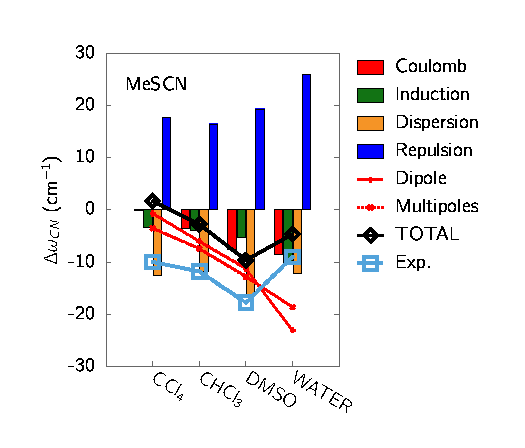
\includegraphics[width=0.9\linewidth]{Fig.5.eps}
}
\caption{
The ensemble\hyp{}averaged values of the frequency shifts of CN stretch mode of MeSCN dissolved in four
different solvents at room temperature, that were obtained by applying the SolEFP model of MeSCN CN
stretch mode to the snapshot configurations taken from the QM/CMD trajectories. The experimental data (black
diamonds) are also shown for comparison. In this Table, ``Dipole'' denotes the Stark\hyp{}dipole model (with the
dipole centred at CN mid\hyp{}bond) whereas ``Multipoles'' describes the site\hyp{}distributed field\hyp{}dependent
frequency shift in Eq.~\ref{e:dw-solefp-electric} on page~\pageref{e:dw-solefp-electric}, 
with the solvatochromic multipole moments and polarizabilities distributed over
all atoms and LMO\hyp{}centroids, respectively. Both take into account induction effects.
\label{t:mescn-solefp-md-exp}}
\end{figure}
%
The experimentally measured average nitrile frequency
shifts are cyan squares in Figure~\ref{t:mescn-solefp-md-exp}. 
The total frequency shifts
calculated with SolEFP and CMD simulation methods are black
diamonds in the same figure. Although the differences
between SolEFP and experimental results are found to be non-negligibly
large by about 10~cm$^{-1}$, the overall trend of the
vibrational frequency shift with respect to the solvent polarity
and H-bonding ability is correctly described by the SolEFP
model. In contrast, the Stark\hyp{}dipole theory predicts even a
very large red shift when MeSCN interacts with water
molecules. Here, it should also be noted that the previous ab
initio semi\hyp{}empirical maps for nitrile frequency shift18, 41
cannot describe the relative blue shift of nitrile stretch mode
in water, because they were based on the assumption that the
vibrational solvatochromic frequency shifts are induced by
electrostatic interactions only.

As can be seen in Figure~\ref{t:mescn-solefp-md-exp}, the exchange\hyp{}repulsion
contribution, $\Delta\omega^{\rm Ex-Rep}$, to the nitrile frequency blue shift in
water is about 8 to 10~cm$^{-1}$ larger than those in aprotic
solvents considered here (compare blue bars in Figure~\ref{t:mescn-solefp-md-exp}). To
further understand the H-bond strength\hyp{}dependence of the
nitrile frequency shift, we performed first\hyp{}principles SolEDS
calculations for Me(S)CN--X dimers with X being H$_2$O, MeOH or
CF$_3$CH$_2$OH, which are presented in Table~\ref{t:mescn-soleds}. 
The corresponding molecular structures are depicted in Figure~\ref{f:mescn-soleds}. 
%
\begin{table}[t!]
\caption{
The nature of the frequency shifts of CN stretch mode in various 
H-bonding complexes involving MeCN or MeSCN and H$_2$O, MeOH 
and CF$_3$CH$_2$OH (structures are shown in Figure~\ref{f:mescn-soleds}). 
The frequency shift partitioning was performed by using 
SolEDS//MP2/6-311++G** method. Bond lengths are in Bohr and frequency shifts in
cm$^{-1}$.
\label{t:mescn-soleds}}
\begin{tabular*}{1.0\textwidth}{@{\extracolsep{\fill} } l ccc c ccc}
\hline\hline
                                 & \multicolumn{3}{c}{MeCN}            && \multicolumn{3}{c}{MeSCN}             \\
                                 & H$_2$O &    MeOH  &  CF$_3$CH$_2$OH &&  H$_2$O   &  MeOH   &  CF$_3$CH$_2$OH \\
\hline
$R_{\rm H-bond}$                 & 3.9814 &   3.9570 &  3.7894         &&  3.9569   &  3.9285 &    3.7550       \\ 
$\Delta\omega^{(10)}_{\rm el}$   & -7.32  &    -8.71 &     -19.45      &&  -14.08   &  -15.89 &    -21.12       \\
$\Delta\omega^{\rm HL}_{\rm ex}$ & +32.31 &   +36.63 &     +44.36      &&  +40.60   &  +46.06 &    +58.16       \\
$\Delta\omega^{\rm HF}_{\rm del}$& -10.49 &   -11.29 &     -17.97      &&  -14.06   &  -15.35 &    -23.83       \\
$\Delta\omega^{(12)}_{\rm el,r}$ &  +4.55 &    +3.48 &     +17.76      &&   +7.80   &   +7.20 &     +6.49       \\
$\Delta\omega^{(2)}_{\rm ex}$    &  +6.79 &    +8.40 &      +3.89      &&   +6.23   &   +7.73 &     +9.84       \\
$\Delta\omega^{(20)}_{\rm disp}$ & -10.63 &   -13.51 &     -15.83      &&  -12.64   &  -16.00 &    -20.62       \\
$\Delta\omega^{\rm MP2}$         & \bf{+15.21} & \bf{+15.00} &  \bf{+12.76}   &&  \bf{+13.85} &  \bf{+13.75} & \bf{+8.92} \\
$\Delta\omega^{(10)}_{\rm el}$+
$\Delta\omega^{(12)}_{\rm el,r}$ &  -2.77 &    -5.23 &      -1.69      &&   -6.28   &   -8.69 &    -14.63       \\
$\Delta\omega^{\rm HL}_{\rm ex}$+
$\Delta\omega^{(2)}_{\rm ex}$    & +39.10 &   +45.03 &     +48.25      &&  +46.83   &  +53.79 &    +68.00       \\
$\Delta\omega^{\rm HF}_{\rm del}$+
$\Delta\omega^{(20)}_{\rm disp}$ & -21.12 &   -24.80 &     -33.80      &&  -26.70   &  -31.35 &    -44.45       \\
Full QM                          & \bf{+12.83} & \bf{+12.58} &  \bf{+8}$^{a)}$ && \bf{+10.54} &  \bf{+10.16} & \bf{+2.86} \\
\hline\hline
\end{tabular*}
%
\begin{footnotesize}
$^{a)}$ Partially optimised due to energy optimisation problem.
\end{footnotesize}
\end{table}
%
%
\begin{figure}[t!]
\centering
\setlength\fboxsep{0.4pt}
\setlength\fboxrule{0.5pt}
\fbox{
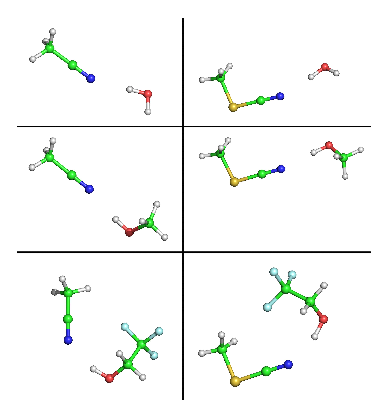
\includegraphics[width=0.92\linewidth]{Fig.S6.eps}
}
\caption{
Molecular structures of the six Me(S)CN--X complexes (X = H$_2$O, MeOH or CF$_3$CH$_2$OH)
that were studied by using SolEDS//MP2/6-311++G** method.
\label{f:mescn-soleds}}
\end{figure}
%
The exchange\hyp{}repulsion
interaction contributes to the very strong frequency
blue shift $\Delta\omega^{\rm HL}_{\rm ex}$. Furthermore, the magnitude of
$\Delta\omega^{\rm HL}_{\rm ex}$
increases as the H-bond length of X molecule increases.
This can be understood by noting that the stronger H-bond
becomes the closer solute and solvent molecules are brought
to each other. This in turn causes a sharp increase in the
exchange\hyp{}repulsion contribution to the frequency shift (see
Figure~\ref{f:mescn-solefp-qm}(b)). This approximately explains all the
frequency blue shifts induced by the interaction between
nitrile and protic solvent molecules, when compared to aprotic
solvents. It is also interesting that, after taking into account
the electron correlation effects
($\Delta\omega^{(12)}_{\rm el,r}$,
$\Delta\omega^{(2)}_{\rm ex}$
and $\Delta\omega^{(20)}_{\rm disp}$ terms in Table~\ref{t:mescn-soleds}), 
the Coulombic effects on the nitrile stretch mode
frequency shifts in these dimers are roughly 6-10 times smaller
than the non\hyp{}Coulombic effects, and the red shifting
contribution is thus due to the charge delocalization and
dispersion interactions. For example, in the case of the
MeSCN-MeOH dimer, the Coulombic frequency shift is just
--8.7~cm$^{-1}$, while the shifts by exchange\hyp{}repulsion effect and
the sum of charge\hyp{}delocalization and dispersion effects are
+53.8 and --31.4~cm$^{-1}$, respectively. The relative contributions
to the frequency shifts from them are similarly found in all the
other dimers studied here (see Table~\ref{t:mescn-soleds}). Therefore, not only
the short\hyp{}range repulsive interaction but also the 
non\hyp{}Coulombic electrostatic effects like induction and dispersion
are also quite important in quantitatively describing the nitrile
frequency shifts in H-bonded systems. Indeed, among the red-shifting
attractive interaction\hyp{}induced contributions, the
dispersion term is dominant, not just in aprotic solvents, but
even in water too (Figure~\ref{t:mescn-solefp-md-exp}). 
Note also that in the case of CCl$_4$,
Coulomb contribution completely vanishes, but yet the
induction contribution is not negligible.

%
\begin{figure}[t!]
\centering
\setlength\fboxsep{0.4pt}
\setlength\fboxrule{0.5pt}
\fbox{
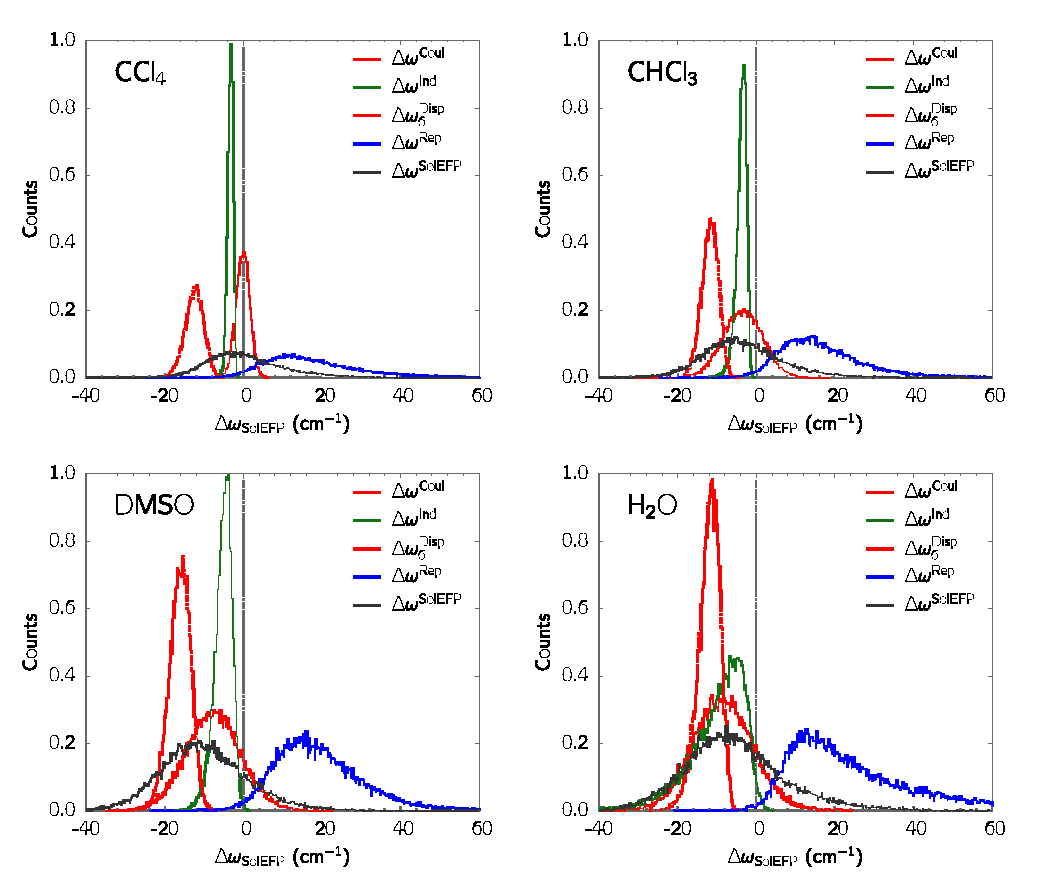
\includegraphics[width=0.9\linewidth]{Fig.6.eps}
}
\caption{
Static frequency shift distributions of CN stretch mode in MeSCN dissolved in four different solvent at room
temperature that were obtained by applying the SolEFP model of MeSCN CN stretch mode to QM/CMD simulation
trajectories.
\label{f:mescn-solefp-md-distr}}
\end{figure}
%
In Figure~\ref{f:mescn-solefp-md-distr}, 
we plot the distributions of different frequency
shift components separately with the full width at half
maximum (FWHM) values listed in Table~\ref{t:mescn-solefp-md-fwhm}. 
%
\begin{table}[t!]
\caption{
Full width at half maximum (FWHM) in cm$^{-1}$ of the distribution of
MeSCN CN stretch mode frequency shift. Frequency shift distributions were
obtained by combining SolEFP method with QM/CMD simulation.
\label{t:mescn-solefp-md-fwhm}}
\begin{tabular*}{1.0\textwidth}{@{\extracolsep{\fill} } l ccccc}
\hline\hline
  & $\Gamma^{\rm Coul}_{\rm static}$
  & $\Gamma^{\rm Ex-Rep}_{\rm static}$
  & $\Gamma^{\rm Ind}_{\rm static}$
  & $\Gamma^{\rm Disp}_{\rm static}$
  & $\Gamma^{\rm SolEFP}_{\rm static}$ \\
\hline
CCl$_4$            &  4.0 $\pm$ 0.5 & 24 $\pm$ 3 & 1.4 $\pm$ 0.5 & 5.6 $\pm$ 1.0 & 21 $\pm$ 4   \\
CHCl$_3$           & 12.0 $\pm$ 0.5 & 21 $\pm$ 3 & 2.5 $\pm$ 1.5 & 5.1 $\pm$ 1.0 & 22 $\pm$ 4   \\
DMSO               & 16.4 $\pm$ 0.5 & 23 $\pm$ 3 & 4.8 $\pm$ 1.5 & 6.4 $\pm$ 1.0 & 25 $\pm$ 4   \\
H$_2$O             & 18.2 $\pm$ 0.5 & 23 $\pm$ 5 & 12.9 $\pm$ 3.0& 6.2 $\pm$ 1.5 & 27 $\pm$ 5   \\
\hline\hline
\end{tabular*}
%
%\begin{footnotesize}
%$^{a)}$
%\end{footnotesize}
\end{table}
%
The distributions
(blue curve in Figure~\ref{f:mescn-solefp-md-distr}) 
of exchange\hyp{}repulsion frequency shifts
are quite broad for all four solutions. As the solvent polarity
increases from CHCl$_3$ to water, the red\hyp{}shifting Coulomb
contribution (red curve) increases. However, the dispersion
contribution remains more or less the same. From the present
SolEFP results shown in Figures~\ref{t:mescn-solefp-md-exp} 
and \ref{f:mescn-solefp-md-distr}, it is quite clear now
that the nitrile frequency shift cannot be fully described by the
contributions, $\Delta\omega^{\rm Coul}$ and $\Delta\omega^{\rm Ind}$, 
that are linearly dependent on
electric field.



\section{SCN Label at the Interface of Two Proteins\label{s:scn-protein-interfac}}

In the above Sections, we showed that the vibrational
solvatochromism of CN probes originates not only from the
electrostatic interaction with solvent electric field but also
from other short\hyp{}range effects that \emph{cannot} be directly
correlated with solvent electric field. In particular, the
exchange\hyp{}repulsion contribution caused by the steric contacts
of the IR probe with surrounding molecules or chemical groups
causes a strong blue shift of the nitrile stretch modes and the
dispersion interaction\hyp{}induced term makes it red\hyp{}shifted. Such
delicate balance among many different contributions to the
vibrational frequency shift is particularly important when
those IR probes are incorporated into proteins. To study these
aspects in detail, one needs to construct a rigorous vibrational
solvatochromism model for protein environment, which
properly takes into account Coulomb, induction, dispersion,
and exchange\hyp{}repulsion interaction\hyp{}induced terms
systematically. Here, we make the first attempt to develop
such \emph{ab initio} model.

\subsection{Constructing the Model for a Protein Environment\label{s:scn-protein-interfac-model-environ}}

This task is
extremely challenging because, unlike the simple cases of
MeSCN in various bulk solutions, we need to consider
vibrational probe which is covalently attached to the
macromolecule (denoted as Prot-SCN) -- note that there is no
well\hyp{}defined theoretical procedure to decouple any IR probe
vibration from the protein backbone. However, we believe
that the vibrational solvatochromism of any Prot-SCN probe
can still be modelled, to a reasonable level of accuracy, by
using the model MeSCN molecule because CN stretch modes
are fairly localised and isolated from other intramolecular
protein vibrations.

To test the transferability of the \emph{ab initio}\hyp{}calculated SolEFP
solvatochromic parameters we studied a few SCN probe
systems embedded in model amino acids of which structures
can be found in the upper panel of Figure~\ref{f:mescn-prot-struct}. 
%
\begin{figure}[t!]
\centering
\setlength\fboxsep{0.4pt}
\setlength\fboxrule{0.5pt}
\fbox{
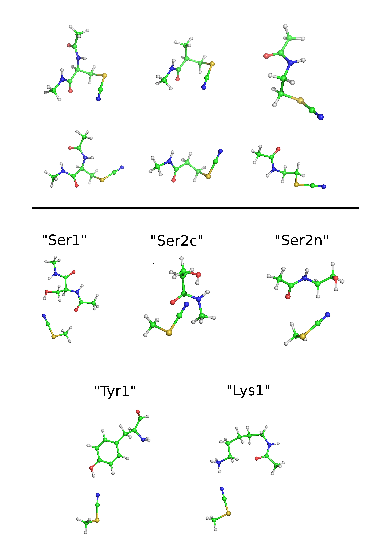
\includegraphics[width=0.98\linewidth]{MeSCN-Prot.struct.eps}
}
\caption{
\emph{Upper:} Structures of six Prot-SCN model compounds.
\emph{Lower:} Structures of MeSCN-peptide dimers used for testing the EFP fragmentation
scheme.
\label{f:mescn-prot-struct}}
\end{figure}
%
We assume that the vibrational
frequency shift induced by neighbouring peptide groups could
be described by the following two factors: (i) Coulombic
frequency shift due to the electric field by the distributed
charges on the amide group (CONH); and (ii) through\hyp{}bond
effects that are associated with frequency shift originating
from change of relative configuration of covalently bonded
chemical group such as methylene. The first effect (i) can be
modelled by considering the interaction of MeSCN
vibrational solvatochromic multipoles with atomic partial
charges of CONH group. The second effect (ii) cannot be
directly quantified, but we could approximately estimate its
nature by performing additional analyses of the CN stretch
mode frequencies of several MeSCN analogs,
where the relative configuration of neighbouring methylene (or
methyl) groups are different from one another. 
This is shown in Figure~\ref{f:mescn-prot-through-bond}(a). 
%
\begin{figure}[t!]
\centering
\setlength\fboxsep{0.4pt}
\setlength\fboxrule{0.5pt}
\fbox{
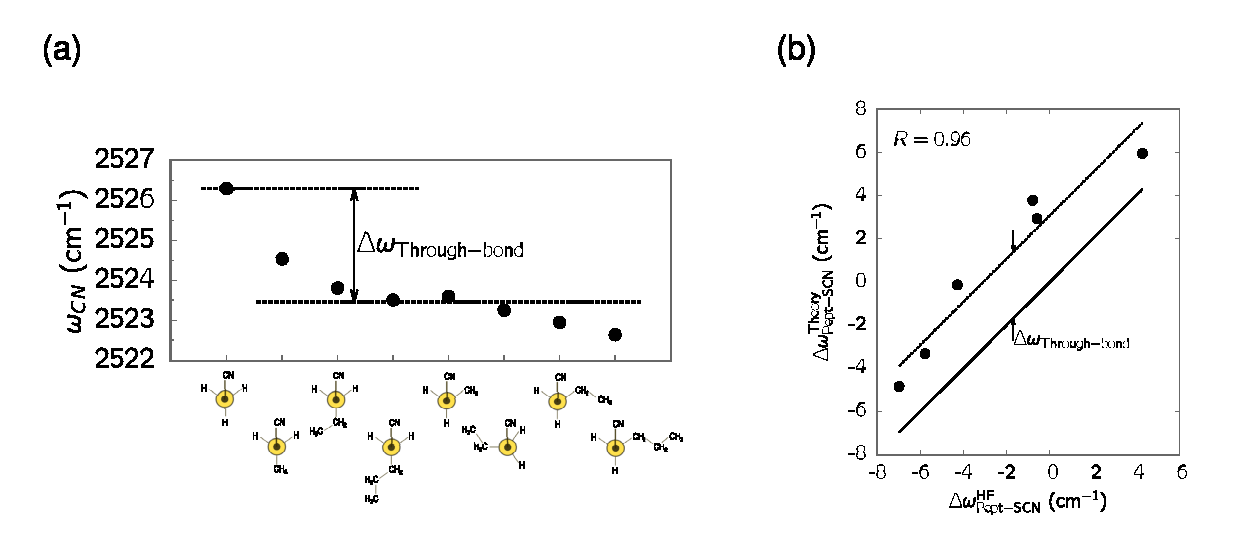
\includegraphics[width=0.98\linewidth]{Fig.8.eps}
}
\caption{
Through-bond effect on CN frequency shift. (a) The CN stretch mode frequency depends on the length and
configuration of the attached aliphatic chain. (b) For a few representative model peptides containing SCN IR
probe (see upper panel of Figure~\ref{f:mescn-prot-struct}), 
we carried out HF/6-311++G** vibrational analyses and the resulting frequency shifts are
compared with the approximate Equation~\ref{e:dw-pept-scn}.
\label{f:mescn-prot-through-bond}}
\end{figure}
%
If one more
methyl (methylene) group is added to the MeSCN, the CN
stretch mode frequency is red\hyp{}shifted by about 3 cm$^{-1}$. Thus,
the overall frequency shift of Prot-SCN due to the local side chain
configuration of Prot-SCN such as proteins with
cyanylated cysteine residues and the two neighbouring amide
groups of the cyanylated cysteine can be approximately
written as
%
\begin{equation} \label{e:dw-pept-scn}
 \Delta\omega_{\text{Pept-SCN}} = \Delta\omega_{\text{MeSCN-CONH}}^{\rm Coul} + \Delta\omega_{\text{Through-bond}}
\end{equation}
%
where $\Delta\omega_{\text{MeSCN-CONH}}^{\rm Coul}$
is evaluated from the interaction of
SolCAMM with ESP charges fitted on $N$-methylacetamide
(NMA) peptide group (see Appendix~\ref{a:nma-esp-fit} for details). Using the above
scheme, we could calculate the vibrational frequency shifts
and compare them with \emph{ab initio} calculation results in Figure~\ref{f:mescn-prot-through-bond}(b). 
The correlation is very good. The constant offset, which is
roughly equal to --3.1~cm$^{-1}$, can indeed be attributed to the
through\hyp{}bond (or additional methylene group) effect, which is
fully consistent with the through\hyp{}bond effect (shifting the
frequency by --2.8~cm$^{-1}$ on average) traced 
in Figure~\ref{f:mescn-prot-through-bond}(a) when
the methyl group of MeSCN is replaced with ethyl or even
longer alkyl chain. The results here show that the SolEFP
parameters extracted from the ab initio calculations of MeSCN
can indeed be used to describe the vibrational
solvatochromism of any Prot-SCN's.

The next and perhaps the more difficult task is to model
the vibrational solvatochromic influences of surrounding
amino\hyp{}acid side chains in protein on the CN frequency of Prot-SCN. 
To use our SolEFP approach, a properly chosen set of
building blocks that faithfully mimic the amino\hyp{}acid side chains
as well as the remaining peptide groups are need. Here we use
the following procedure: i) the aliphatic group of side chain is
represented by an appropriately superimposed methane; 
ii) the aromatic side chain of phenylalanine is by benzene; 
iii) the histidine side chain is modelled by imidazole; iv) polar groups
can be modelled by the methylated group (for example MeOH
is the model for the serine side chain); and v) the peptide bond is
modelled by NMA. 
%
\begin{table}[t!]
\caption{
The minimalistic model of amino acid side chains that is used in Eq.~\ref{e:dw-solefp-prot}.
In this model, the protein is mimicked by a set of small EFP2 fragments that
capture the fundamental physical components of the interaction between the IR
probe and molecular environment. Peptide units are treated by NMA molecules
except those two being attached next to SCN probes (see the main text).
\label{t:solefp-prot-residues}}
\begin{tabular*}{1.0\textwidth}{@{\extracolsep{\fill} } ||l|l|l||}
\hline\hline
Aminoacid side-chain     & EFP2 fragments                    & Modelled fragment \\
\hline
\multirow{1}{*}{Asp}     & \textbullet CH$_3$COO$^-$         & \textbullet Carboxyl group (deprotonated) \\ \hline
\multirow{2}{*}{Asn}     & \textbullet CHONH$_2$             & \textbullet Amide group \\
                         & \textbullet CH$_4$                & \textbullet C$\beta$H$_2$ \\ \hline
\multirow{2}{*}{Glu}     & \textbullet CH$_3$COO$^-$         & \textbullet Carboxyl group (deprotonated) \\
                         & \textbullet CH$_4$                & \textbullet C$\beta$H$_2$ \\ \hline
\multirow{2}{*}{Gln}     & \textbullet CHONH$_2$             & \textbullet Amide group \\
                         & \textbullet 2 $\times$ CH$_4$     & \textbullet C$\beta$H$_2$, C$\gamma$H$_2$ \\ \hline
\multirow{1}{*}{Ser}     & \textbullet CH$_3$OH              & \textbullet C-OH group \\ \hline
\multirow{2}{*}{Thr}     & \textbullet CH$_3$OH              & \textbullet C-OH group \\ 
                         & \textbullet CH$_4$                & \textbullet C$\beta$H$_2$ \\ \hline
\multirow{2}{*}{Tyr}     & \textbullet PhOH                  & \textbullet Ar-OH group \\
                         & \textbullet CH$_4$                & \textbullet C$\beta$H$_2$ \\ \hline
\multirow{2}{*}{Phe}     & \textbullet Benzene               & \textbullet Aromatic ring \\
                         & \textbullet CH$_4$                & \textbullet C$\beta$H$_2$ \\ \hline
\multirow{2}{*}{Lys}     & \textbullet CH$_3$NH$_3^+$        & \textbullet Amine group (protonated) \\
                         & \textbullet 3 $\times$ CH$_4$     & \textbullet C$\beta$H$_2$, C$\gamma$H$_2$, C$\delta$H$_2$ \\ \hline
\multirow{2}{*}{Arg}     & \textbullet Methylguanidinium$^+$ & \textbullet Guanidinium group (protonated) \\
                         & \textbullet 2 $\times$ CH$_4$     & \textbullet C$\beta$H$_2$, C$\gamma$H$_2$ \\ \hline
\multirow{1}{*}{Gly}     & -                                 & - \\ \hline
\multirow{2}{*}{His}     & \textbullet Imidazole             & \textbullet Imidazole ring (not protonated) \\
                         & \textbullet CH$_4$                & \textbullet C$\beta$H$_2$ \\ \hline
\multirow{2}{*}{Trp}     & \textbullet Indole                & \textbullet Indole group \\
                         & \textbullet CH$_4$                & \textbullet C$\beta$H$_2$ \\ \hline
\multirow{2}{*}{Met}     & \textbullet (CH$_3$)$_2$S         & \textbullet Methyl sulfide group \\
                         & \textbullet CH$_4$                & \textbullet C$\beta$H$_2$ \\ \hline
\multirow{1}{*}{Cys}     & \textbullet CH$_3$SH              & \textbullet C-SH group \\ \hline
\multirow{1}{*}{Pro}     & \textbullet 3 $\times$ CH$_4$     & \textbullet Ring \\ \hline
\multirow{1}{*}{Ala}     & \textbullet CH$_4$                & \textbullet C$\beta$H$_2$ \\ \hline
\multirow{1}{*}{Leu}     & \textbullet 3 $\times$ CH$_4$     & \textbullet \emph{sec}-buthyl chain \\ \hline
\multirow{1}{*}{Ile}     & \textbullet 3 $\times$ CH$_4$     & \textbullet 2-methyl-$n$-propyl chain \\ \hline
\multirow{1}{*}{Val}     & \textbullet 3 $\times$ CH$_4$     & \textbullet \emph{iso}-propyl chain \\
\hline\hline
\end{tabular*}
%
%\begin{footnotesize}
%$^{a)}$
%\end{footnotesize}
\end{table}
%
In Table~\ref{t:solefp-prot-residues}, 
the model chemical groups
representing twenty amino acids are summarised and we
obtained the EFP2's of those model compounds. One of the
problems originates from the overlap between an EFP2
fragment and an NMA modelling an amide group. Here, we
assume that the `spurious' atoms introduced by all of the
EFP2's do not contribute much to the vibrational frequency
shift. Then, we adopt the following strategy:
%
\begin{itemize}
 \item The SolEFP pairwise\hyp{}additive frequency shifts originating
from Coulomb, dispersion, and exchange\hyp{}repulsion
interactions between model amino acid side chains and
nitrile are evaluated by using the standard SolEFP method
described here.
 \item The (polarization) induction effects are included as
follows: the vibrational frequency shifts due to the
interaction of nitrile with all the overlapping fragments
such as CH$_4$ and NMA are considered separately. The
remaining fragments including polar fragments as well as
solvent water molecules are considered by taking into
account the many\hyp{}body induction effects.
\end{itemize}
%
This scheme is formulated as
%
\begin{equation} \label{e:dw-solefp-prot}
 \Delta\omega^{\rm SolEFP} \approx 
 \left(
   \sum_{\rm X}^{\text{all EFP2's}}
    \Delta\omega_{\text{Solute-X}}^{\rm Coul}
   +\Delta\omega_{\text{Solute-X}}^{\rm Ex-Rep}
   +\Delta\omega_{\text{Solute-X}}^{\rm Disp}
 \right)
  + \Delta\omega^{\rm Ind}
\end{equation}
%
where
%
\begin{equation} \label{e:dw-solefp-prot-ind}
 \Delta\omega^{\rm Ind} \approx
  \Delta\omega^{\rm Ind}_{\text{Polar EFP2's}} + 
    \sum_{\rm X}^{\text{remaining EFP2's}}
      \Delta\omega_{\text{Solute-X}}^{\rm Ind}
\end{equation}
%
To test the validity of the above approach, 
Eqs.~\ref{e:dw-solefp-prot} and \ref{e:dw-solefp-prot-ind},
we specifically considered five dimeric complexes consisting of
one MeSCN and serine, tyrosine, or lysine model peptide which are shown
in lower panel of Figure~\ref{f:mescn-prot-struct}. 
First, we carried out \emph{ab initio} harmonic
vibrational analyses of those complexes to obtain the CN
frequency shifts. Then, we utilised the fragment approach with the
SolEFP parameters of MeSCN and the EFP2's representing the
serine, tyrosine, and lysine model peptides and the results
are shown in Table~\ref{t:solefp-prot-fragmentation}. 
%
\begin{table}[t!]
\caption{
Test of the EFP fragmentation model used in the minimalistic model of the protein
(Table~\ref{t:solefp-prot-residues}). 
In this Table, the test protein environment mimicking molecules [``Ser1'', ``Ser2c'',
``Ser2n'', ``Tyr1'', ``Lys1''; see the structures above in Figure~\ref{f:mescn-prot-struct}] 
are treated by SolEFP
method. First, the interaction with an entire EFP parameter (``Full'') set is considered. Then,
the same molecules are approximated by small EFP models and Eq.~\eqref{e:dw-solefp-prot} 
is used to evaluate
SolEFP shifts (``Frag''). To test our solvatochromic theory we also show more accurate
SolEDS calculations in this table and compare it with ``Full QM'' frequency shifts, those
which were obtained from harmonic normal mode analysis. To compare SolEFP results with
SolEDS at HF level, the SolEFP frequency shifts without dispersion ($\Delta\omega^{\rm SolEFP}_{\text{no disp}}$) 
are presented
here as well. Note that, while the SolEDS method takes into account both mechanical and
electronic anharmonicities for all the interaction energy contributions, in the SolEFP method
the electronic anharmonicity is included only for $\Delta\omega^{\rm Coul}$ 
(see Section~\ref{s:solefp-working-model}). 
All calculations were performed at HF/6-311++G** level of
theory.
\label{t:solefp-prot-fragmentation}}
\begin{tabular*}{1.0\textwidth}{@{\extracolsep{\fill} } ll ccccc }
\hline\hline
&& ``Ser1'' & ``Ser2c'' & ``Ser2n'' & ``Tyr1'' & ``Lys1'' \\
\multicolumn{7}{c}{SolEFP} \\ \hline
\multirow{2}{*}{$\Delta\omega^{\rm Coul}$}     & Frag &   -8.3   &  -5.9   &   -7.7   &   -5.7   & -39.9   \\
                                               & Full &   -9.0   &  -7.2   &  -10.8   &   -6.7   & -38.3   \\
\multirow{2}{*}{$\Delta\omega^{\rm Ex-Rep}$}   & Frag &   24.9   &  14.4   &   10.3   &   24.4   &  70.0   \\
                                               & Full &   24.0   &  14.9   &   11.1   &   22.5   &  72.7   \\
\multirow{2}{*}{$\Delta\omega^{\rm Ind}$}      & Frag &   -6.1   &  -4.4   &   -4.1   &  -10.8   & -46.9   \\
                                               & Full &   -7.4   &  -8.0   &   -6.4   &  -14.6   & -51.0   \\
\multirow{2}{*}{$\Delta\omega^{\rm Disp}_6$}   & Frag &   -6.9   &  -6.3   &   -6.2   &   -4.6   & -13.9   \\
                                               & Full &   -6.1   &  -6.4   &   -6.1   &   -5.0   & -14.9   \\
\multirow{2}{*}{$\Delta\omega^{\rm SolEFP}$}   & Frag &    3.6   &  -2.2   &   -7.7   &    3.3   & -30.7   \\
                                               & Full &    1.5   &  -6.7   &  -12.2   &   -3.8   & -31.5   \\
\multirow{2}{*}{$\Delta\omega^{\rm SolEFP}_{\text{no disp}}$}   
                                               & Frag &   10.5   &   4.1   &   -1.5   &    7.9   & -16.8   \\
                                               & Full &    7.6   &  -0.3   &   -6.1   &    1.2   & -16.6   \\
\multicolumn{7}{c}{SolEDS} \\  \hline
\multicolumn{2}{l}{$\Delta\omega^{(10)}_{\rm el}$}    &  -11.9   & -10.1   &  -11.8   &   -9.7   & -34.5   \\
\multicolumn{2}{l}{$\Delta\omega^{\rm HL}_{\rm ex}$}  &   25.0   &  16.4   &   14.7   &   26.4   &  69.2   \\
\multicolumn{2}{l}{$\Delta\omega^{\rm HF}_{\rm del}$} &  -12.5   &  -8.5   &   -7.6   &  -10.1   & -44.6   \\
\multicolumn{2}{l}{$\Delta\omega^{\rm HF}$}           &    0.6   &  -2.2   &   -4.7   &    6.6   & -10.0   \\
\multicolumn{7}{c}{Full QM} \\  \hline
\multicolumn{2}{l}{$\Delta\omega^{\rm HF}$}           &   -0.5   &  -3.1   &   -5.4   &    5.3   & -10.7   \\
\hline\hline
\end{tabular*}
%
%\begin{footnotesize}
%$^{a)}$
%\end{footnotesize}
\end{table}
%
Surprisingly, the fragment approach reproduces
both $\Delta\omega^{\rm Disp}$ and $\Delta\omega^{\rm Ex-Rep}$ very well. 
Our Eq.~\ref{e:dw-solefp-prot-ind} however
underestimates the induction effect (compare ``Full'' and
``Frag'' entries in Table~\ref{t:solefp-prot-fragmentation}). 
Perhaps this is because the
cooperative induction effects by bonding orbital electrons of
two different fragments were ignored, which is the problem
that cannot be easily resolved and is beyond the scope of the
present work. Nonetheless, our SolEDS//HF frequency shifts are
in excellent agreement with full \emph{ab initio} results with the errors
of just $\sim$1~cm$^{-1}$ or lesser. When dispersion is not included in
SolEFP, those analysis results can be compared to SolEDS//HF
results. Overall, the SolEFP, as compared to the SolEDS,
underestimates the frequency shifts by about 4-10~cm$^{-1}$.
This is mainly due to the approximate nature of the SolEFP
method in taking into account the non\hyp{}Coulombic
interactions. Nevertheless, Eq.~\ref{e:dw-solefp-prot}
works reasonably well, though the present approach is highly
simple and approximate in nature. What is important here is
that the short\hyp{}range repulsion and dispersion effects, which
are often the main contributions to the nitrile frequency shifts
in solutions, are at least correctly described by the present
fragment SolEFP model for vibrational solvatochromism of
nitrile IR probes in protein environments.

%\subsection{Short\hyp{}range frequency shifts of CN stretch in Ras\hyp{}binding
%domain of RalGDS\label{s:ral-solefp}}
\subsection{Vibrational Frequency Shifts Inside Proteins\label{s:ral-solefp}}

To get the detailed insight into the origin of
the short\hyp{}range interaction\hyp{}induced vibrational frequency
shifts of CN probes embedded in proteins, we have specifically
studied the Ral guanine nucleotide dissociation stimulator
(RalGDS), which is a downstream effector of Rap1A (Rap). The
Ras\hyp{}binding domain of RalGDS was systematically mutated at six
different positions to introduce an SCN probe (Figure~\ref{f:prot}).   % 54
Andrew W. Ritchie, who was doing his PhD course in Prof. Lauren J. Webb's 
group in the University of Texas at Austin,
has performed umbrella sampling molecular dynamics
simulations of the six mutants of RalGDS in water and the same
mutants docked to human oncoprotein p21$^{\rm Ras}$ (Ras) mutant
(here labelled as Ras'; see Computations). 
%
\begin{figure}[t!]
\centering
\setlength\fboxsep{0.4pt}
\setlength\fboxrule{0.5pt}
\fbox{
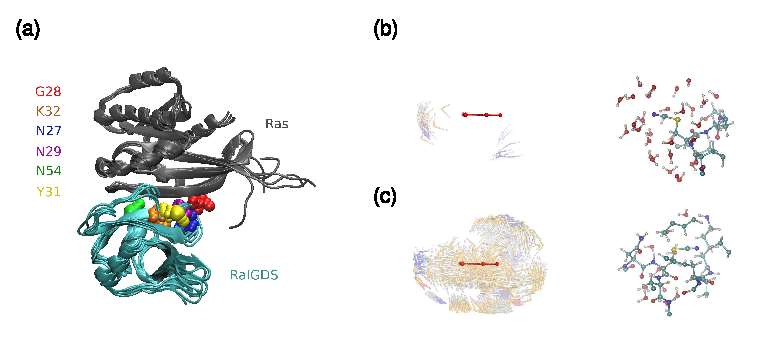
\includegraphics[width=0.98\linewidth]{prot.eps}
}
\caption{
(a) Locations of the SCN probes within RalGDS protein bound to Ras' (Ras D30E{\textunderscore}E31).
(b) and (c) The vicinities of SCN label in free RalGDS at Y31 position (a)
and complex RalGDS/Ras D30E{\textunderscore}E31 at G28 position. The left probability maps show the
non\hyp{}aqueous residues with the transparency approaching zero for the most probable
configurations based on WHAM analysis. The white, brown, red and blue areas around SCN (red balls and sticks
in the middle) 
denote hydrogen, carbon, oxygen and nitrogen atoms of protein environment. The right insets are the representative
snapshots.
}
\label{f:prot}
\end{figure}
%
From
those CMD trajectories, we have considered the local
environments within 10~\AA from SCN probes, 
where the most probable configurations were taken
into consideration based on the weighted histogram analysis
method. In total, about 1000 Prot-SCN configurations were
taken from the CMD trajectories for our SolEFP fragment
analyses. The average values of the short\hyp{}range frequency
shifts of SCN stretch modes in free RalGDS and RalGDS\hyp{}Ras' 
complexes are presented in Figure~\ref{f:radial-plots}
%
\afterpage{
\begin{figure}[t!]
\centering
\setlength\fboxsep{0.4pt}
\setlength\fboxrule{0.5pt}
\fbox{
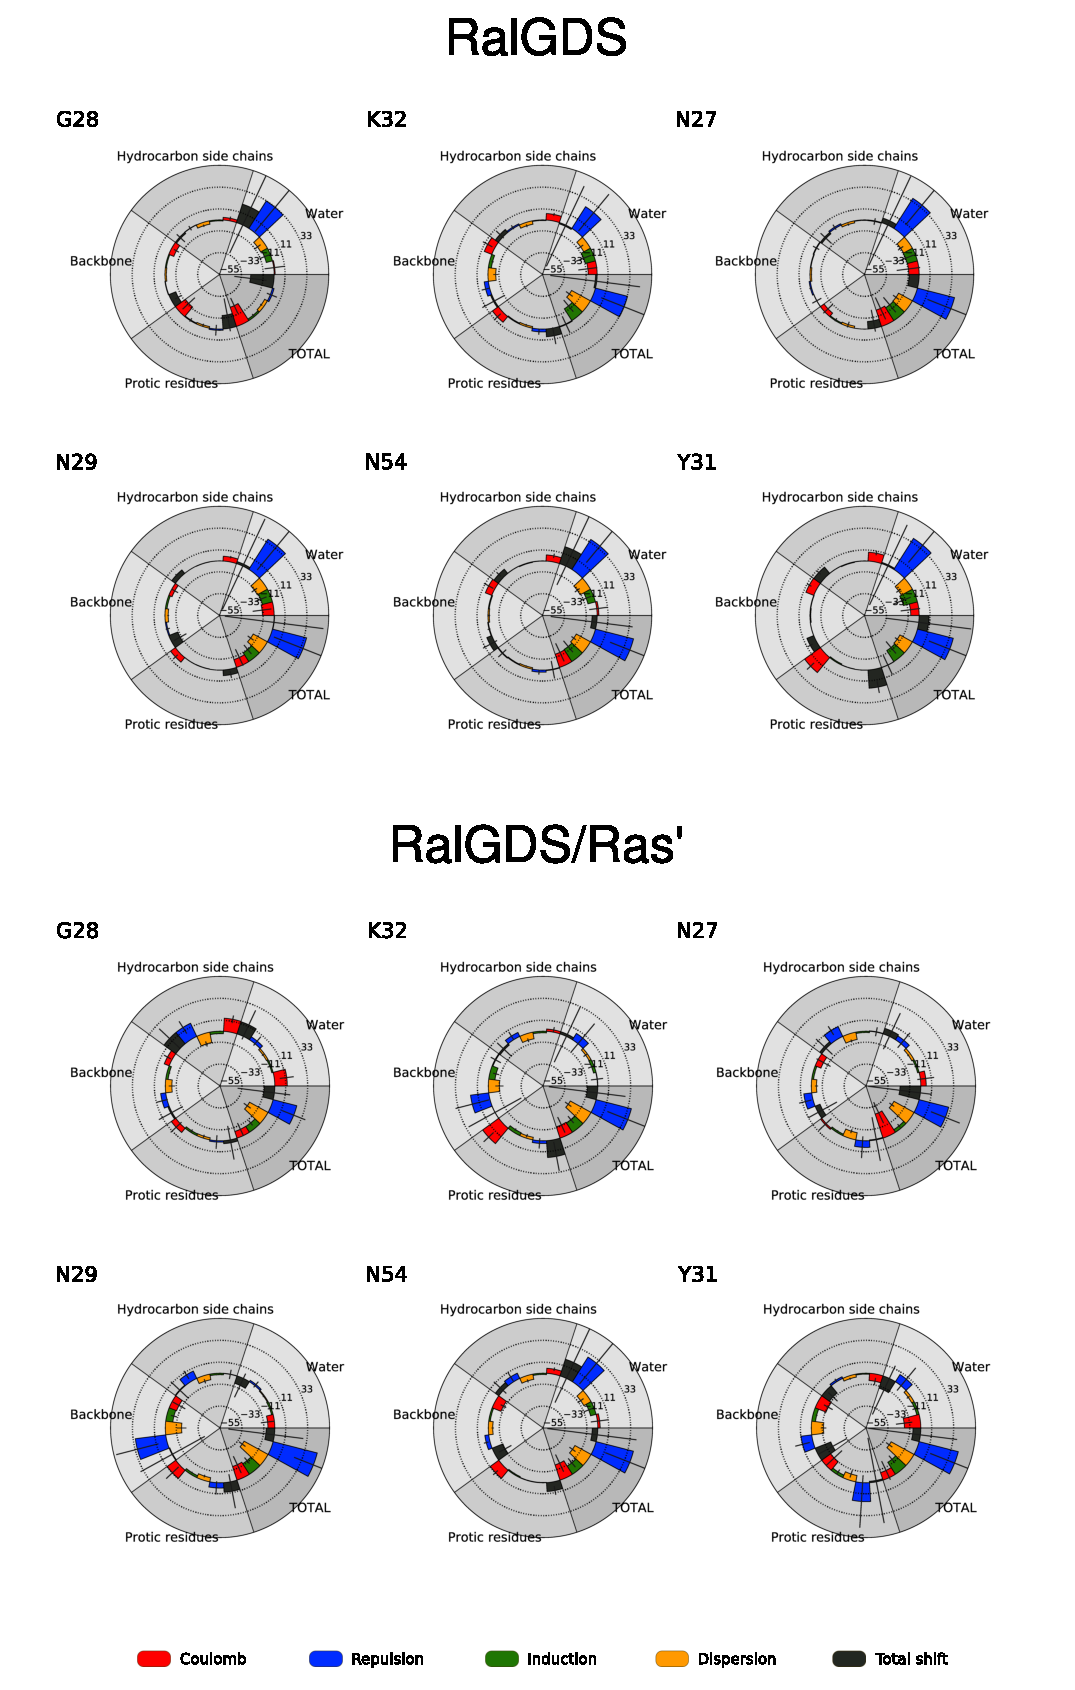
\includegraphics[width=0.9\linewidth]{radial-diag.eps}
}
\caption{
The SolEFP short\hyp{}range frequency shift components of CN stretch mode of SCN probe incorporated at six
different sites of free RalGDS protein (\emph{upper}) and RalGDS that is non\hyp{}covalently bound to Ras'
(\emph{lower}). 
The frequency shifts were averaged
over roughly 80 configurations in each case, taken from the umbrella sampling simulations. Only 
configurations with the highest WHAM probabilities were selected. 
The standard deviations for each frequency shift contribution are
displayed with black error bars. All values in cm$^{-1}$.
}
\label{f:radial-plots}
\end{figure}
\clearpage
}
%

In the cases of RalGDS proteins without binding to Ras',
all the SCN probes are highly exposed to water so
that the contributions from protein environment to the SCN
stretch frequency shifts are relatively small and mainly are
Coulombic in nature. $\Delta\omega^{\rm Ex-Rep}$ due to solvating water molecules
is very large, about 35~cm$^{-1}$. This is even larger than that of
MeSCN in water, which is about 26~cm$^{-1}$ (see Figure~\ref{t:mescn-solefp-md-exp}).
This difference is likely to be caused by the differences in
the force field parameters (of SCN group and water) that were
used to simulate bulk solutions in Section~\ref{s:dw-cn-bulk} and the protein
systems in water. The induction and dispersion effects are
generally similar to those in bulk water and the Coulomb
contribution varies from case to case, because the SCN probes
have quite different orientations with respect to water phase --
note that $\Delta\omega^{\rm Coul}$ is strongly dependent on the angle between
SCN and H-bonded water molecule.

The situation is much more complicated when SCN probe is
located at the interface of RalGDS and Ras' proteins. 
The calculated $\Delta\omega^{\rm Ex-Rep}$ values are still quite large, which
range from +24 cm$^{-1}$ in RalGDS/G28+Ras' to +40~cm$^{-1}$ in
RalGDS/Y31+Ras'. Furthermore, the blue shifts have quite
different origins depending on the specific position of the SCN
probe. Non\hyp{}bonding close\hyp{}contact of SCN with aliphatic or
aromatic part of amino acid side chain (Val, Leu, Ile or Phe) is
the dominant interaction contributing to $\Delta\omega^{\rm Ex-Rep}$ in the case of
G28. On the other hand, in the cases of K32 and N29, the
interaction of SCN with protein backbone induces a substantial
blue shift, where the H-bond between SCN and amide proton
and the repulsive interaction between peptide\hyp{}oxygen and
SCN-nitrogen atoms are important. In the case of Y31, SCN
probe is located in the vicinity of Ser residues that form strong
hydrogen bonds through OH groups with SCN and induce a
substantial blue shift. It is interesting to note here that when
Ras' protein is not docked to RalGDS, SCN probe does not
make such H-bonding interaction with Ser residue because, in
that case, the probe prefers to interact with water rather than
protein. This results in a lack of the exchange\hyp{}repulsion blue
shift due to Ser. Also, in the case of RalGDS/G28 (without
docked protein), SCN interacts with Tyr residue via making an
H-bond with OH group of Tyr. However, typical H-bond
lengths, estimated from the CMD trajectory, are longer than
those of RalGDS/Y31+Ras' so that the exchange\hyp{}repulsion
interaction\hyp{}induced frequency shift due to the tyrosine OH
group is small (note that $\Delta\omega^{\rm Ex-Rep}$ is a very short\hyp{}range effect
and becomes vanishingly small as solute\hyp{}solvent distance
increases; Figure~\ref{f:mescn-solefp-qm}(b). %and also Appendix~\ref{}). % add graphs from R_max scans for MeSCN in four solvents
Finally, the SCN probe in the case of
N54 can form H-bonding interactions with water molecules
penetrated into the protein-protein interface, which induces a
strong blue shift. This is an exceptional position at the RalGDS
protein that is likely to be exposed to water in both free and
bound states of RalGDS, whereas the SCN group at the other
positions does not form a H-bonding interaction with water
molecules when RalGDS binds to the Ras mutant studied here.

It is clear that both water and protein residues can cause
a large blue shift of SCN stretch frequency due to their
exchange\hyp{}repulsion interactions with SCN. Another distinctive
feature found here is that the dispersion effects are generally
larger at the protein interface (by about 5 to 10~cm$^{-1}$), when
compared with those in the cases of free RalGDS proteins. This
is mainly because many\hyp{}electron hydrocarbon groups including
aromatic rings are close to the SCN probe in the cases of
RalGDS--Ras complexes. Unfortunately, our calculations of the
SCN frequency shifts in RalGDS proteins cannot be directly
compared with experimental results previously reported in
Refs. \citep{Stafford.Ensign.Webb.JPCB.2010,Ritchie.Webb.JPCB.2013,Ritchie.Webb.JPCB.2015} 
since our Prot-SCN CMD simulation systems considered in
this work are still too small because of the short cut\hyp{}off
distance of 10~\AA used in the present Coulombic interaction\hyp{}induced
frequency shift calculation. Furthermore, it should be noted
that the experimentally measured frequency shifts differ from
one another by at most 3~cm$^{-1}$ -- note that none of the existing
vibrational solvatochromic maps have this chemical accuracy
yet. Therefore we do not aim to reproduce those relative
frequency shifts in this work. Rather, our qualitative analysis
results presented here shows the importance of the exchange-repulsion
and the dispersion interaction effects, which cannot
be described with other electric field\hyp{}based theories previously
used. Our results suggest also that the magnitudes of
$\Delta\omega^{\rm Ex-Rep}$ at the protein surface are larger than those in bulk
solutions. Interestingly, the repulsion effects are quantitatively
similar in both aqueous and protein environments (note that
$\Delta\omega^{\rm Ex-Rep}$ of CN stretch mode of MeSCN in water is higher by
about 7~cm$^{-1}$ than that in DMSO, CHCl$_3$ or CCl$_4$). The spatial
confinement effects at the interface between RalGDS and Ras'
proteins is of particular importance because the environment
around SCN is crowded and congested, which results in a
strong repulsion interaction. Only in the case of
RalGDS/G28+Ras', the repulsion frequency shift is smaller
than 30~cm$^{-1}$. From this, it is shown that the frequency blueshift
due to the H-bonding interactions of SCN with water
molecules cannot be distinguished from that to the repulsive
interactions of SCN with protein residues.

We have to mark here that the amount of protein samples
taken from CMD is very little at a present time (roughly 80-100
CMD snapshots per system) so that a further study along this
line is necessary. Still, we believe that most of the probable
configurations based on the weighted histogram analysis
method were taken into consideration in the present
calculation study and that most of the salient features about
the distribution of the frequency shifts of CN IR probe
embedded in a highly heterogeneous protein environment
were captured here. Nevertheless, it will be desirable to carry
out further works for comparatively small proteins to test the
validity of the SolEFP approach developed here.



\section{Effects of Atom Order Reversal Within CN Group\label{s:cn-nc}}

In a recent study of Maj~\emph{et al.}, \citep{Maj.Ahn.Blasiak.Kwak.Han.Cho.XXX.2016} 
it was demonstrated that the
isonitrile (N$\equiv$C) vibrational frequency is remarkably sensitive
towards H-bonding whereas almost constant in aprotic solvents 
of varying polarity. Moreover, it was shown that the extinction coefficient
of the NC stretch mode 1$\leftarrow$0 transition is much greater
(up to 14 times for aliphatic and 2.4 times for aromatic
derivatives) as compared with the corresponding nitrile analogue.

To explain the molecular origins of such greatly enhanced sensitivity towards H-bonding 
interactions, we carried out extensive QM calculations of interaction energy decomposition, 
from which individual contributions to vibrational shift were determined based on recently 
developed model of solvatochromism. For the study, we chose two simple models of 
acetonitrile and methyl isocyanide, hydrogen\hyp{}bonded to a water and chloroform molecule. 
The results showing each interaction energy contributions to vibrational frequency shift are 
given in Table~\ref{t:cnnc-soleds}, whereas the molecular structures are depicted in Figure~\ref{f:cnnc-soleds-str}.
%
\begin{table}[t!]
\caption{SolEDS//HF/6-311++G** frequency shifts of the CN/NC stretch mode with
respect to gas phase that were computed for the model solute\hyp{}solvent systems 
(Figure~\ref{f:cnnc-soleds-str}). The 
lengths of hydrogen bonds are shown in parentheses below the system label.
Exact frequency shifts (``Full QM'') computed for the fully 
optimised structures are also shown.
Frequency shift values are given in cm$^{-1}$.
\label{t:cnnc-soleds}}
\begin{tabular*}{1.0\textwidth}{@{\extracolsep{\fill} } l cccc}
\hline\hline
              & MeCN--H$_2$O & MeNC--H$_2$O & MeCN--CHCl$_3$ & MeNC--CHCl$_3$ \\
              & R$_{\rm NH}$ = 2.245\AA 
              & R$_{\rm CH}$ = 2.421\AA 
              & R$_{\rm NH}$ = 2.375\AA 
              & R$_{\rm CH}$ = 2.575\AA \\
\hline
$\Delta\omega^{(10)}_{\rm el}$       & --4.6   &  +9.0    &  --5.3         &  +7.8  \\
$\Delta\omega^{\rm HL}_{\rm ex}$     & +16.0   & +14.3    & +8$\pm$4*      & +11.7  \\
$\Delta\omega^{\rm HF}_{\rm del}$    & --4.9   & --2.8    & $\sim$0$\pm$4* & --1.3  \\
$\Delta\omega^{\rm SolEDS}$          &  +6.5   & +20.5    &   +4.4         & +18.2  \\
\hline
Full QM                              &  +5.9   & +20.1    &   +4.1         & +18.0  \\
\hline\hline
\end{tabular*}
\end{table}
%
\begin{figure}[b!]
\centering
\setlength\fboxsep{0.4pt}
\setlength\fboxrule{0.5pt}
\fbox{
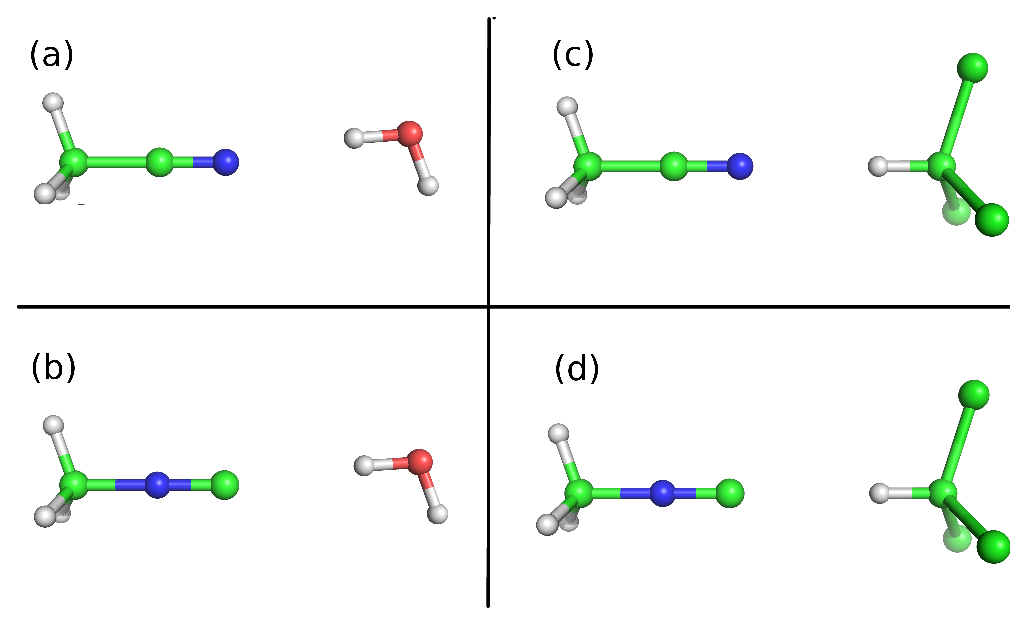
\includegraphics[width=0.9\linewidth]{cnnc.SolEDS.structures.eps}
}
\caption{
Molecular structures of the model systems used for SolEDS//HF/6-311++G**
analyses. (a) MeCN--H$_2$O (b) MeNC--H$_2$O (c) MeCN--CHCl$_3$ and (d) MeNC--CHCl$_3$
\label{f:cnnc-soleds-str}}
\end{figure}
%
It is clear that the 
frequency blue\hyp{}shifts due to (both proper and improper) H-bond are significantly larger in the 
case of isocyanide probes, with the almost four\hyp{}fold increase in frequency shift as compared
to the gas\hyp{}phase states of MeCN and MeNC. It is interesting that the origins of these 
frequency shifts in terms of the exchange\hyp{}repulsion and charge\hyp{}delocalization effects are 
virtually the same. On the other hand, the first\hyp{}order electrostatic contribution (which is 
mostly due to the multipolar interactions) changes its sign in the case of isonitriles causing 
the electrostatic blue shift instead of red shift. Note that this change in sign enforces blue 
shifts due to exchange\hyp{}repulsion in stark contrast to the nitrile frequency shift where 
Coulombic and exchange\hyp{}repulsion cancel one another. To understand this sign change in the 
Coulombic contribution to the vibrational frequency shifts of isonitrile stretch mode we have 
computed the \emph{ab initio} solvatochromic vibrational multipole moments (SolMMM) 
of CN/NC stretches which are shown in Table~\ref{t:cnnc-solcamm}.
%
\begin{table}[t!]
\caption{Solvatochromic dipole and quadrupole moments of CN/NC stretches of
acetonitrile (MeCN) and methyl isocyanide (MeNC) in cm$^{-1}$/(MV/cm) and 10$^{-8}\times$\
cm$^{-1}$/(MV/cm$^2$), respectively. Principal symmetry axes of all the molecules are collinear with 
$z$-axis so that $x$ and $y$ dipole as well as $xy$, $xz$, $yz$ quadrupole components vanish. 
$z$-axis is 
pointing towards N atom in nitrile or C atom in isonitrile group, respectively. Solvatochromic 
quadrupole has its origin in CN or NC mid\hyp{}bond.
\label{t:cnnc-solcamm}}
\begin{tabular*}{1.0\textwidth}{@{\extracolsep{\fill} } ll ccc c ccc}
\hline\hline
Method & Basis set    & \multicolumn{3}{c}{MeCN} && \multicolumn{3}{c}{MeNC}                 \\
       &              & \multicolumn{7}{c}{\emph{ab initio}}                                 \\
       &              & $z$     &  $xx=yy$  & $zz$     &&    $z$    &  $xx=yy$    &    $zz$  \\
\cline{3-5} \cline{7-9}
B3LYP  & 6-311++G**   & $-$0.29  &  $-$0.54   &  +1.08   &&   +0.28   &   $-$0.42    &   +0.85  \\
HF     & 6-311++G**   & $-$0.38  &  $-$0.54   &  +1.09   &&   +0.38   &   $-$0.38    &   +0.77  \\
MP2    & 6-311++G**   & $-$0.059 &  $-$0.43   &  +0.86   &&   +0.014  &   $-$0.51    &   +1.02  \\
CCSD   & 6-311++G**   & $-$0.19  &  $-$0.47   &  +0.93   &&   +0.22   &   $-$0.44    &   +0.87  \\
CCSD   & aug-cc-pVDZ  & $-$0.18  &  $-$0.50   &  +1.00   &&   +0.25   &   $-$0.45    &   +0.90  \\
CCSD   & aug-cc-pVTZ  & $-$0.19  &  $-$0.48   &  +0.96   &&   +0.24   &   $-$0.42    &   +0.85  \\
%\hline
       &              & \multicolumn{7}{c}{Fitting}                                             \\
       &              & $z$      &  $xx=yy$   & $zz$     &&    $z$    &  $xx=yy$     &    $zz$  \\
\cline{3-5} \cline{7-9}
B3LYP  & 6-311++G** 
                      &          &            &          &&   +0.57   &   $-$1.32    &   +2.64  \\
B3LYP  & 6-311++G(3df,2pd) 
                      &  --0.32$^{a)}$ &  --1.23$^{a)}$  & +2.47$^{a)}$  && & &              \\
%\hline
       &              & \multicolumn{7}{c}{Exp.$^{b)}$}                                      \\
       &              & \multicolumn{3}{c}{$\vert z\vert$}    && \multicolumn{3}{c}{$\vert z\vert$} 
                                                                                             \\
\cline{3-5} \cline{7-9}
       &              & \multicolumn{3}{c}{0.33--0.39$^{c)}$} && \multicolumn{3}{c}{-}       \\
\hline\hline
\end{tabular*}
\begin{footnotesize}
$^{a)}$ Ref.~\citep{Lee.Choi.Cho.JCP.2012}, 
$^{b)}$ Ref.~\citep{Andrews.Boxer.JPCA.2000}, 
$^{c)}$ assuming that the local field correction factor is between 1.1--1.3.
\end{footnotesize}
\end{table}
%

Generally, the B3LYP and HF values of ${\BM \upmu}_{\rm CN}$ are in good agreement with experiment.
For
instance, the B3LYP/6-311++G** \emph{ab initio} calculation and B3LYP/6-311++G(3df,2pd) 
empirical estimation give the absolute magnitudes of 0.29 and 0.32 cm$^{-1}$/(MV/cm), 
respectively, with the experimental range of 0.32--0.39 cm$^{-1}$/(MV/cm). Interestingly, MP2 
significantly underestimates the absolute magnitude of the CN solvatochromic dipole which 
is predicted to be less than 0.06 cm$^{-1}$/(MV/cm) in its absolute magnitude. The fact that 
HF level provides correct order of magnitude (0.38 cm$^{-1}$/(MV/cm)) is surprising and 
apparently more refined electron\hyp{}correlation method than MP2 is necessary in the case of 
correlated \emph{ab initio} calculations. Using CCSD method gives the result with correct order of magnitude and
our best \emph{ab initio} estimations of MeCN CN and MeNC NC Stark tuning rates are 0.19 and
0.24 cm$^{-1}$/(MV/cm) at CCSD/aug-cc-pVTZ level, respectively.
Unfortunately, there are no available measurements of ${\BM \upmu}_{\rm NC}$
for MeNC in the literature. Nevertheless, all of our \emph{ab initio} and empirical estimates 
consistently show that ${\BM \upmu}_{\rm CN}$ and ${\BM \upmu}_{\rm NC}$ 
point in the opposite directions along the
corresponding CN/NC bond axes. Note also that the vibrational quadrupole, unlike dipole, is 
not affected much by flipping C and N atoms within IR probe.
Therefore, the differences in the
sign of $\Delta\omega^{(10)}_{\rm el}$
are caused primarily by the reversal the corresponding solvatochromic 
dipole directions.

To understand the reasons behind the significantly enhanced intensities of NC probes over
CN probes, we have analysed the dipole derivatives with respect to XY (XY = NC or CN) stretch
modes, $\fderiv{{\BM \upmu}}{Q_{\rm XY}} \Bigg|_{{\bf Q}_{0}}$,
since the IR intensities are proportional to its modulus squared.
Assuming that
%
\begin{equation}
 {\BM \upmu} \approx \sum_x^{\rm atoms} q_x {\bf r}_x 
\end{equation}
%
where $q_a$ and ${\bf r}_x$ are the position and partial charge of $x$th atom, respectively,
the dipole derivative can be expressed as a sum of the two contributions
%
\begin{equation} \label{e:torii-partitioning}
 \fderiv{{\BM \upmu}}{Q_{\rm XY}} \Bigg|_{{\bf Q}_{0}} \approx
 \sum_x^{\rm atoms} \fderiv{q_x}{Q_{\rm XY}} \Bigg|_{{\bf Q}_{0}} {\bf r}_x 
  +
 \sum_x^{\rm atoms} q_x \fderiv{{\bf r}_x}{Q_{\rm XY}} \Bigg|_{{\bf Q}_{0}}
 \equiv 
 \partial {\BM \upmu}_{\rm XY}^{\rm cf} + \partial {\BM \upmu}_{\rm XY}^{\rm vib}
\end{equation}
%
In the above equation, $\partial {\BM \upmu}_{\rm XY}^{\rm cf}$ denotes the
charge\hyp{}flow term due to the charge density
redistribution that occurs during the vibrational displacement of atoms, 
whereas $\partial {\BM \upmu}_{\rm XY}^{\rm vib}$
associated with the structural character of the vibration itself. 
Note that, in the case of XY
stretches, the vibrational motion is dominated by the change 
in XY bond length. The 
partitionings according to Eq.~\eqref{e:torii-partitioning} 
were performed for C-XY (C = CH$_3$ or phenyl), and the 
results are shown in Table~\ref{t:cnnc-mu-part}.
%
\begin{table}[t!]
\caption{Charge\hyp{}flow $\left( \partial {\BM \upmu}_{\rm XY}^{\rm cf} \right)$
and structural\hyp{}vibrational $\left( \partial {\BM \upmu}_{\rm XY}^{\rm vib} \right)$
1$^{\rm st}$ derivative with respect to XY (XY = NC or CN) stretch normal coordinate 
that were obtained by using MP2/6-311++G** method combined with ChelpG atomic charge 
analysis (Eq.~\eqref{e:torii-partitioning}). 
Principal symmetry axes of all the molecules are collinear with $z$-axis so that $x$ and $y$ 
components vanish. $z$-axis is pointing towards N atom in nitrile or C atom in isonitrile group, 
respectively. Positive (negative) sign of $Q_{\rm XY}$ corresponds to XY bond elongation (stretching). 
Analytical dipole derivative (``Full QM'') is also presented in this table for the sake of 
comparison. All values are in a.u. 
\label{t:cnnc-mu-part}}
\begin{tabular*}{1.0\textwidth}{@{\extracolsep{\fill} } l cccc}
\hline\hline
                                          & MeCN      & MeNC     & PhCN     & PhNC     \\
\hline
%
& \multicolumn{4}{c}{MP2/6-311++G**}                                                   \\
$\partial\mu_{z,{\rm XY}}^{\rm cf}$       &   +0.60   &   +1.64  &   +0.54  &   +1.94  \\
$\partial\mu_{z,{\rm XY}}^{\rm vib}$      &  --0.62   &  --0.59  &  --0.59  &  --0.63  \\
$\fderiv{\mu_z}{Q_{\rm XY}}$              &  --0.02   &   +1.05  &  --0.05  &   +1.31  \\
Full QM                                   &  --0.0008 &  +1.0616 & --0.0585 & +1.2955  \\
%
& \multicolumn{4}{c}{CCSD/6-311++G**}                                                  \\
$\partial\mu_{z,{\rm XY}}^{\rm cf}$       &   +0.48   &   +1.92  &   +0.26  &  +2.37   \\
$\partial\mu_{z,{\rm XY}}^{\rm vib}$      &  --0.62   &   -0.55  &  --0.60  & --0.58   \\
$\fderiv{\mu_z}{Q_{\rm XY}}$              &  --0.14   &   +1.38  &  --0.35  &  +1.79   \\
Full QM                                   &  --0.1447 &  +1.3895 & --0.3435 & +1.8010  \\
%
& \multicolumn{4}{c}{CCSD/aug-cc-pVDZ}                                                 \\
$\partial\mu_{z,{\rm XY}}^{\rm cf}$       &   +0.45   &   +1.87  &   +0.29  &  +1.91   \\
$\partial\mu_{z,{\rm XY}}^{\rm vib}$      &  --0.60   &  --0.52  &  --0.63  & --0.15   \\
$\fderiv{\mu_z}{Q_{\rm XY}}$              &  --0.14   &   +1.35  &  --0.35  &  +1.76   \\
Full QM                                   &  --0.1428 &  +1.3645 & --0.3444 & +1.7701  \\
%
& \multicolumn{4}{c}{CCSD/aug-cc-pVTZ}                                                 \\
$\partial\mu_{z,{\rm XY}}^{\rm cf}$       &   +0.42   &   +1.91  &    -     &  -       \\
$\partial\mu_{z,{\rm XY}}^{\rm vib}$      &  --0.61   &  --0.55  &    -     &  -       \\
$\fderiv{\mu_z}{Q_{\rm XY}}$              &  --0.20   &   +1.36  &    -     &  -       \\
Full QM                                   &  --0.1955 &  +1.3603 &    -     &  -       \\
\hline\hline
\end{tabular*}
\end{table}
%
From our analyses it is clear that the structural contribution is 
very similar in all the studied model systems but the charge\hyp{}flow contribution is substantially 
increased in the case of NC probes. To get a deeper insight into the origins of this increase we 
have plotted the 3D map of the electron density flow, $\fderiv{\rho}{Q_{\rm XY}} \Bigg|_{{\bf Q}_{0}}$, 
in Figure~\ref{f:cnnc-maps}.
%
\begin{figure}[t!]
\centering
\setlength\fboxsep{0.4pt}
\setlength\fboxrule{0.5pt}
\fbox{
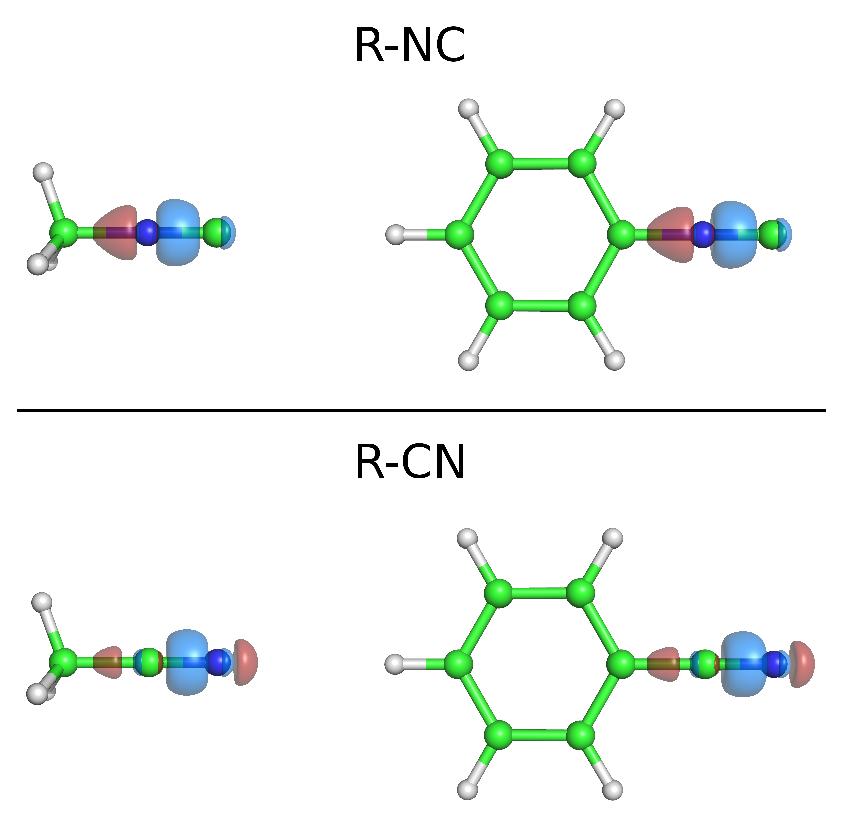
\includegraphics[width=0.9\linewidth]{cnnc.map.mp2.iso-0.20.eps}
}
\caption{
First derivatives of the electron density distribution $\left( \fderiv{\rho}{Q_{\rm XY}} \Bigg|_{{\bf Q}_{0}} \right)$
with respect to CN/NC stretch mode calculated at the MP2/6-311++G** level. 
Positive (negative) sign of $Q_{\rm XY}$
corresponds to elongation (stretching) of the CN or NC bonds. The iso-contours were 
plotted for $\pm$0.2~a.u. with red and blue colours representing positive and negative values, 
respectively.
\label{f:cnnc-maps}}
\end{figure}
%

Obviously, as the
the XY bond length increases ($Q>0$), the electron density on XY bond decreases. However, 
when NC bond is elongated, there is a notable density flow from carbon lone pair and NC 
bond towards N--C(H$_3$) bond (mechanism `I'). In contrast, in the case of CN bond elongation 
the density flows from CN bond in two opposite directions: towards C--C(H$_3$) bond 
(mechanism `I') and towards nitrogen lone pair (mechanism `II'). This indicates that the net 
charge flow is dictated by the position of the more electronegative (nitrogen) atom in XY group 
which results in much smaller $\partial {\BM \upmu}_{\rm XY}^{\rm cf}$ contribution in the case of
nitrile stretching vibration,
and in turn, in a very small dipole derivative. This explains the significant increase in the 
intensity of NC stretch absorption relative to CN stretch in both aliphatic and aromatic 
(iso)nitriles. This phenomenon might be also responsible for the sign reversal in the
solvatochromic dipole of NC stretch mode because ${\BM \upmu}_{\rm XY}$ is approximately proportional to
%
\begin{equation}
 {\BM \upmu}_{\rm XY} \propto \fderiv{{\BM \upmu}}{Q_{\rm XY}} \Bigg|_{{\bf Q}_{0}} 
    \qquad\text{(approximately)}
\end{equation}
%
We believe that the interaction energy decomposition scheme and the electron density
analysis presented in this study may be useful approach to study origins of the vibrational
solvatochromism and intensity enhancements of many different molecular probes.


\section{Discussion}

\subsection{Origins of the Vibrational Frequency Shifts of CN Stretch Mode}

Our analysis is consistent with the previous empirical
calculation of the CN stretch mode of acetonitrile \citep{Reimers.Hall.JACS.1999}, 
in which
Reimers and Hall found, by applying the solvent descriptor
model of Fawcett~\emph{et al.} \citep{Fawcett.Liu.Kessler.JPC.1993}, 
that the dispersion interaction
contributes the most to the observed frequency red shifts.
They also found a drastic increase in ``specific'' frequency blue
shifts as they were using more protic solvents like water, 
2,2,2\hyp{}trifluoroethanol and trifluoroacetic acid. For instance, the nonspecific
electrostatic, dispersion and specific (electrostatic and
non-electrostatic) frequency shifts of CN mode of acetonitrile
in water were found to be --6.4, --9.7 and +6.7~cm$^{-1}$, whereas in
CCl$_4$ --1.9, --13.0 and 0.0~cm$^{-1}$, respectively. Therefore, it is
evident that those short\hyp{}range blue\hyp{}shifting effects originate
from the exchange\hyp{}repulsion interactions that were previously
analysed by Rey and Hynes \citep{Rey.Hynes.JCP.1998} 
and Morales and Thompson \citep{Morales.Thompson.JPCB.2011}
from a perspective of a repulsive part of the van der Waals
intermolecular potential.

\subsection{Does Stark-Dipole Theory Describe Induction Effects Accurately?\label{s:stark-dipole-cn}}

It is necessary to point out the limitation of the
vibrational Stark theory. 
In the paragraph on page~\pageref{p:solindmult} we showed that the
evaluation of the solvatochromic induced dipole and quadrupole moments is
straightforward within the SolEFP theory, and are given by Eqs.~\eqref{e:34e1} and \eqref{e:34e2}.
Assuming Stark\hyp{}dipole model the frequency shift
is
%
\begin{equation} \label{e:dmtp-solmmm-dipole}
 \Delta\omega_j^{\rm Elect} \approx  -
                       \left\{ {\bf L}_j + \frac{1}{2} {\bf L}_j^{\rm ind} \right\} 
                       \cdot {\bf F}({\bf r}_0) = {\bf L}_j^{\rm Stark} \cdot {\bf F}({\bf r}_0)
\end{equation}
%
with ${\bf L}_j^{\rm Stark}$ denoting the effective Stark tuning rate.
In fact, the induction part of ${\bf L}_j^{\rm Stark}$ depends on the electric field.
Therefore, the ensemble\hyp{}averaged vibrational frequency shift
is
%
\begin{equation} 
 \langle \Delta\omega_j^{\rm Elect} \rangle =  -
                        {\bf L}_j  \cdot  \langle  {\bf F}({\bf r}_0) \rangle 
                     - \frac{1}{2} \langle {\bf L}_j^{\rm ind}  \cdot {\bf F}({\bf r}_0) \rangle
\end{equation}
%
The dot product in last term in the above equation need to be averaged out.
In order to make such an extended Stark\hyp{}dipole model (that handles also induction)
applicable for experimentalist, we are forced to approximate this second term
by assuming that solvatochromic induced dipole ${\bf L}_j^{\rm ind}$ does not
changes its direction much due to thermal fluctuations of the solvent molecules around.
In other words,
%
\begin{equation} \label{e:dmtp-solmmm-dipole-assumption} 
\langle {\bf L}_j^{\rm ind}  \cdot {\bf F}({\bf r}_0) \rangle \approx 
{\bf L}_j^{\rm ind} \cdot  \langle  {\bf F}({\bf r}_0) \rangle 
\qquad \text{(assumption)}
\end{equation}
%
When the polarizability projected onto
the bond axis of nitrile is taken into consideration,
the electric field\hyp{}induced vibrational frequency
shift takes the approximate form reported by 
Fried~\emph{et al.} \citep{Fried.Wang.Boxer.Ren.Pande.JPCB.2013}
%
\begin{equation}  \label{e:extended-stark-model}
\langle \Delta\omega_j^{\rm Elect} \rangle \approx - L_j^{\rm Stark} F
\end{equation}
%
In the above equation, the modified Stark tuning rate, which includes the
induction term approximately, is given as
%
\begin{equation}  
L_j^{\rm Stark}  = L_j + \frac{1}{2} \langle L_j^{\rm Ind} \rangle
\end{equation}
%
Since
the SolEFP approach is the first\hyp{}principles theory that includes
all the vibrational solvatochromic induced multipole moments,
we could test the validity of the extended but still approximate
expression for the Stark\hyp{}dipole model in Eq.~\eqref{e:extended-stark-model}. 

\begin{table}[t!]
\caption{
Frequency shifts originating from the Coulomb interaction and induction 
(polarization) contributions of CN stretch mode of MeSCN in four different solvents. 
Here,
the exact SolEFP induction frequency shift is compared with the approximate schemes 
(see the main text for explanation). The vibrational solvatochromic dipole and
quadrupole magnitudes are presented in the last two columns. ${\bf F}$ denotes 
the set of electric fields at nineteen distributed sites of MeSCN whereas ${\bf F}_{\rm CN}$ 
is the electric field at the CN
mid\hyp{}bond. Frequency shifts are given in cm$^{-1}$ and solvatochromic dipoles and quadrupoles 
in cm$^{-1}$/(MV/cm) and $10^{-8}\times$ cm$^{-1}$/(MV/cm$^2$), respectively.
\label{t:stark-dipole-ind}}
\begin{tabular*}{1.0\textwidth}{@{\extracolsep{\fill} } l cccc c cc}
\hline\hline
 &\multicolumn{4}{c}{Frequency shifts}  && \multicolumn{2}{c}{Multipoles}\\
\cline{2-5} \cline{7-8} 
  & $\Delta\omega_{\rm CN}^{\rm Coul}$ & $\Delta\omega_{\rm CN}^{\rm Ind}$ 
  & $\langle-\frac{1}{2}\langle{\BM\upmu}_{\rm CN}^{\rm Ind}\rangle\cdot{\bf F}_{\rm CN}\rangle$
  & $\langle-\frac{1}{2}\langle{\bf a}_{\rm CN}'\rangle\cdot{\bf F}\rangle$
 && $\lvert\langle{\BM\upmu}_{\rm CN}\rangle\rvert$
  & $\lvert\langle{\BM\Theta}_{\rm CN}\rangle\rvert$ \\
\hline
Vacuum     &      0.0  &   0.0  &  0.0 &  0.0  &&  0.466 &  1.16 \\
CCl$_4$    &     -0.7  &  -3.3  &  0.0 &  0.0  &&  0.436 &  1.05 \\
CHCl$_3$   &     -5.6  &  -3.8  &  0.0 & -0.6  &&  0.477 &  1.05 \\
DMSO       &    -10.6  &  -5.2  & -0.2 & -1.6  &&  0.506 &  1.07 \\
H$_2$O     &    -18.5  & -10.1  & -3.2 & -4.3  &&  0.639 &  1.04 \\
\hline\hline
\end{tabular*}
%
%\begin{footnotesize}
%$^{a)}$
%\end{footnotesize}
\end{table}
%
In Table~\ref{t:stark-dipole-ind}, we compare the exact induction frequency
shifts that can be calculated with Eq.~\eqref{e:dw-ind-avec} with (i) those
obtained by considering time\hyp{}averaged vibrational
solvatochromic induced dipole in Eq.~\eqref{e:extended-stark-model} interacting with the
instantaneous electric field evaluated at the CN mid\hyp{}bond, i.e.,
$\langle-\frac{1}{2}\langle{\BM\upmu}_{\rm CN}^{\rm Ind}\rangle\cdot{\bf F}_{\rm CN}\rangle$
and (ii) those obtained by
considering time\hyp{}averaged vibrational solvatochromic induced
dipoles distributed over nineteen different locations in MeSCN
molecule that interact with the instantaneous electric fields at
those polarizable sites, i.e., 
$\langle-\frac{1}{2}\langle{\bf a}_{\rm CN}'\rangle\cdot{\bf F}\rangle$
(see Eq.~\eqref{e:dw-ind-avec}). In addition, the total magnitudes of the
solvatochromic dipole and quadrupole moments, as well as
the Coulomb frequency shifts (Eq.~\eqref{e:dw-solefp-coul-working}), 
are also given in Table~\ref{t:stark-dipole-ind}.

As can be seen in Table~\ref{t:stark-dipole-ind}, it is concluded that the exact
induction frequency shift $\Delta\omega_{\rm CN}^{\rm Ind}$ 
in Table~\ref{t:stark-dipole-ind}) cannot be
reproduced by the two approximate calculation methods (i)
and (ii) discussed above. To examine the directionality of the
vibrational solvatochromic induced dipoles, we examined the
relative orientation of the total vibrational solvatochromic
induced dipole with respect to the permanent vibrational
solvatochromic dipole of the nitrile stretch mode (Figure~\ref{f:solv-dip-directionality}(a)). 
%
\begin{figure}[t!]
\centering
\setlength\fboxsep{0.4pt}
\setlength\fboxrule{0.5pt}
\fbox{
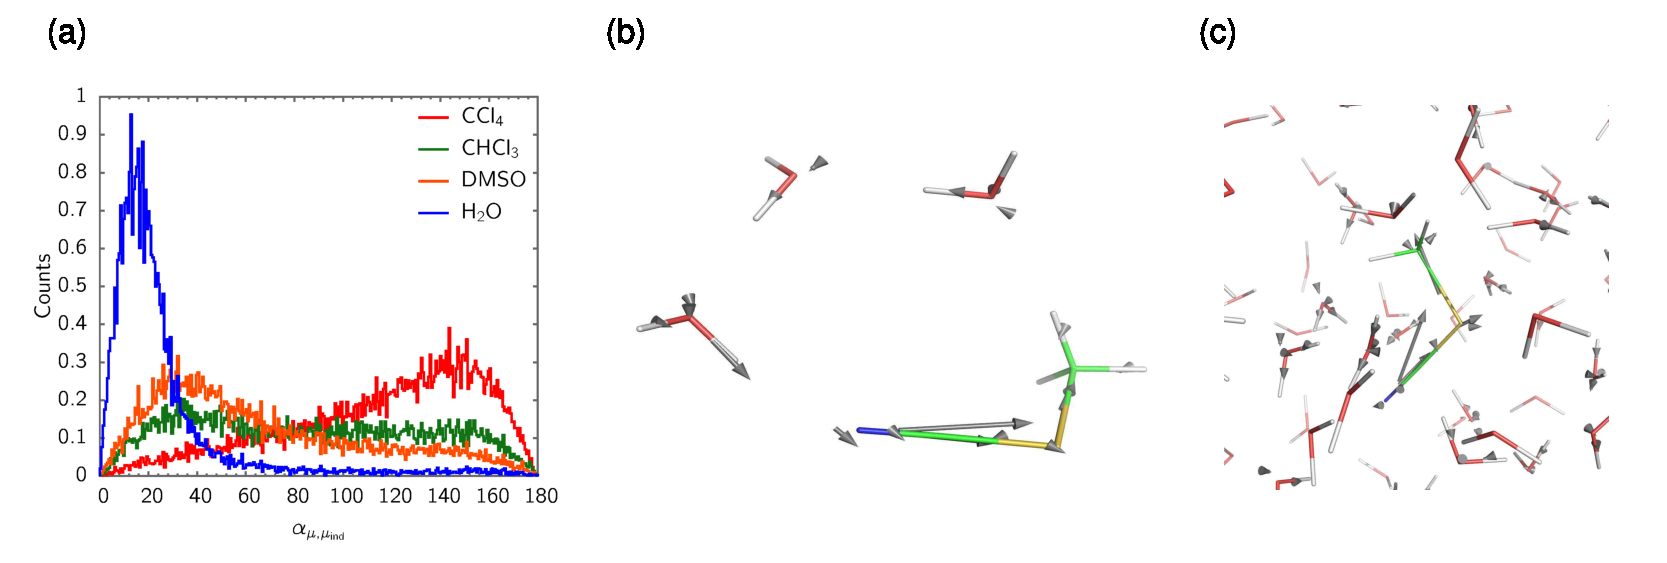
\includegraphics[width=0.98\linewidth]{Fig.7.with.eps}
}
\caption{
(a) The distributions of the angles between the induced molecular solvatochromic
dipole moments of CN stretch mode in MeSCN with the static solvatochromic dipole,
centred at CN mid\hyp{}bond. The analysis was performed by applying the SolEFP model of
MeSCN CN stretch mode to QM/CMD simulation trajectories. Angles are given in degrees.
(b) and (c) Vibrational solvatochromic (SolEFP) induced dipole moments 
(gray arrows, ${\bf a}'$ in Eq.~\eqref{e:avec-prime}) of CN stretch
mode of MeSCN interacting with water molecules. Note that the induced dipoles are delocalized even on
water molecules: (b) A cluster consisting of MeSCN and three water molecules. (c) A configuration taken
from QM/CMD trajectory.
\label{f:solv-dip-directionality}}
\end{figure}
%
It turns out that the relative angle between the two
dipoles varies from 0 to 180\textdegree in all the aprotic solvents. This
means that the induction frequency shifts are determined by
instantaneous solute\hyp{}solvent configurations so that the
averaged value over all possible solute\hyp{}solvent configurations
cannot provide information on local electric field [note that
the total magnitudes of the molecular vibrational
solvatochromic dipoles and quadrupoles do not depend on
solvent much (see Table~\ref{t:stark-dipole-ind})]. However, in the case of water, the
vector component of the average induced vibrational
solvatochromic dipole is large and it induces small red shift
(Table~\ref{t:stark-dipole-ind}). This indicates that the extended Stark\hyp{}dipole theory
including both the molecular vibrational solvatochromic dipole
and solvent\hyp{}induced dipole contributions \citep{Fried.Wang.Boxer.Ren.Pande.JPCB.2013} 
is still incapable of
fully describing even the induction effects correctly in the
cases of nitrile probes. To prove this quantitatively, for both a
small cluster consisting of one MeSCN and three water
molecules (Figure~\ref{f:solv-dip-directionality}(b)) and a large cluster taken from QM/CMD
trajectory (Figure~\ref{f:solv-dip-directionality}(c)), we calculated the instantaneous distributed
vibrational solvatochromic dipoles (${\bf a}_j'$ in Eq.~\eqref{e:dw-ind-avec-alternative}) 
and depict
them with arrows. 
%%
%\begin{figure}[t!]
%\centering
%\setlength\fboxsep{0.4pt}
%\setlength\fboxrule{0.5pt}
%\fbox{
%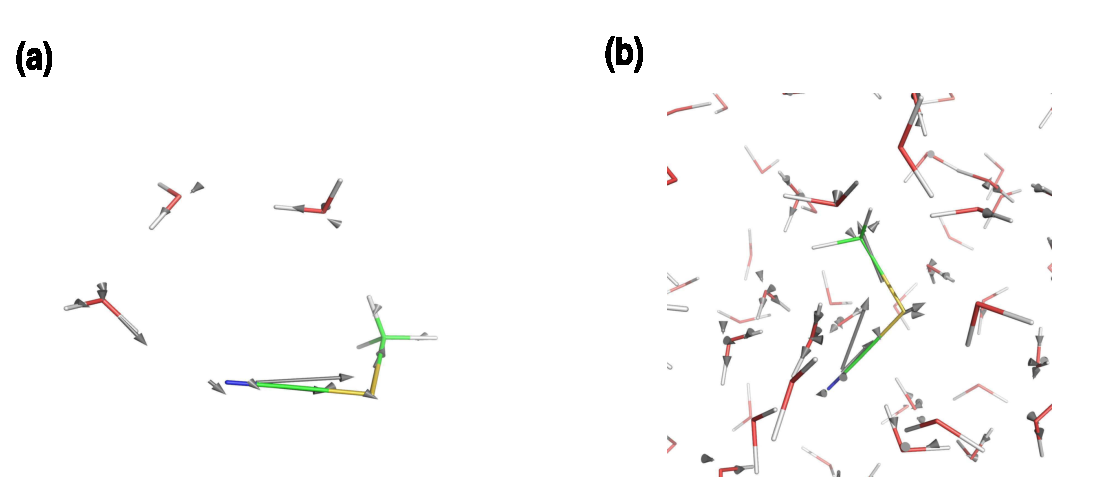
\includegraphics[width=0.9\linewidth]{Fig.7.eps}
%}
%\caption{
%
%\label{f:mescn-aj}}
%\end{figure}
%%
Note that quite a few dipoles at different
sites contribute to $\Delta\omega_{\rm CN}^{\rm Ind}$, 
where they all have quite different
directions and magnitudes. If they all are added up at the midpoint
of the CN bond, they would largely cancel out with one
another. Furthermore, they are spatially delocalized even on
surrounding water molecules so that $\Delta\omega_{\rm CN}^{\rm Ind}$
cannot be simply
estimated by considering the induced dipoles of MeSCN only.
We emphasise that the SolEFP induction theory fully takes into
account such non\hyp{}additive nature in calculating $\Delta\omega^{\rm Ind}$ 
and that
${\bf a}_j'$ \emph{spans the entire system} including both solute and solvent
molecules. \citep{Blasiak.Cho.JCP.2014} 
Therefore, it becomes clear that the Stark\hyp{}dipole
model is a highly approximate approach to predict the
frequency shifts of nitrile stretch mode not only because it
does not include other important contributions from
vibrational solvatochromic quadrupolar, exchange\hyp{}repulsion
and dispersion effects, but also because it does not take into
account even the induction effect correctly. Indeed, the assumption
from Eq.~\eqref{e:dmtp-solmmm-dipole-assumption} appears to be \emph{incorrect}.

\subsection{CN Probes Inside Proteins}

One of the related works was reported by Zou~\emph{et al.} By carrying
out CMD simulations, they obtained van der Waals and
electrostatic forces exerting on the CN group of benzonitrile
embedded at four different sites in a model ion channel
protein to elucidate the origins of the CN frequency change
caused by the binding of halothane molecule. \citep{Zou.Liu.Blasie.BiophysJ.2009} 
They found that
electrostatic forces are roughly 2--2.5 times larger in magnitude
than van der Waals forces and they used Stark dipole model
for further analyses. The agreement with average
experimental value of the frequency shift (about 6~cm$^{-1}$) was
found to be quite good (roughly 3 and 6~cm$^{-1}$ obtained from
two separate CMD simulations). However, their approach does
not provide all the contributions to the vibrational frequency
shifts separately. In fact, their analysis of the van der Waals
forces included not only blue\hyp{}shifting exchange\hyp{}repulsion but
also red\hyp{}shifting dispersion effect that have opposite signs and
very different distance\hyp{}dependencies [dispersion is a relatively
long\hyp{}range effect as compared to exchange\hyp{}repulsion; see
Fig.~\ref{f:mescn-solefp-md-dist}]. 
Therefore, the actual importance of the non\hyp{}Coulombic 
frequency shifts was not traced fully in the study of
Zou~\emph{et al.} \citep{Zou.Liu.Blasie.BiophysJ.2009}  
due to the cancellation of attractive and repulsive
contributions that result in the frequency shifts of different
nature.

Recently, Zhang~\emph{et al.} have proposed a new IR probe based on
5-cyanoindole that was found to be a good candidate for
monitoring the local dynamics in proteins, especially because
of its sensitivity to the molecular environment and notably
long vibrational lifetime (12.3~ps for the ground state bleach
decay). \citep{Zhang.Markiewicz.Doerksen.Smith.Gai.PCCP.2015} 
However, they showed that the vibrational response
of their probe is governed by the local molecular environment
around CN group, i.e., intermolecular H-bonds with CN group,
and intramolecular coupling of CN with indole's NH group. This
cannot be easily modelled by the Stark dipole theory.
Moreover, it is expected that even the contemporary
(empirical or first\hyp{}principles) solvatochromic maps based on
the distributed site multipoles \citep{Waegele.Gai.JCPL.2010,
Lee.Choi.Cho.JCP.2012,Blasiak.Lee.Cho.JCP.2013} might have faced certain
problems in quantitatively describing the vibrational frequency
shifts of such IR probes due to the complicate nature of H-bonding
interaction in general. We believe that the SolEFP
model along with its protein\hyp{}model extension presented in this
work for the first time is a promising first step toward
developing more refined and chemically accurate model
capable of capturing all the vibrational solvatochromic effects
from many\hyp{}body intermolecular interactions, especially when
an IR probe is surrounded by highly heterogeneous molecular
environments like proteins.


\section{Summary}

In this study, we have analysed the solvatochromic vibrational
frequency shifts of nitrile stretch mode in a variety of different
molecular environments by using the first principles SolEFP
model. Our model is
capable of reproducing the relative experimental vibrational
frequency shifts of CN stretch of MeSCN dissolved various solvents. 
The
electric\hyp{}field\hyp{}based theories cannot properly describe the CN
vibrational frequency shift induced by H-bonding interaction of
water molecules because they ignored the exchange\hyp{}repulsion
effect that causes a strong frequency blue shift.
In addition, we here showed that the dispersion interaction
between polarizable CN group and polarizable solvent
molecules is yet another important red\hyp{}shifting contribution to
the frequency shift. Therefore, Stark\hyp{}dipole
theory is highly inappropriate in case of CN probes. 
Our extended vibrational solvatochromism
theory was used to elucidate the origin of CN frequency shifts
of SCN probes in highly heterogeneous protein environments. We found that 
the exchange\hyp{}repulsion frequency
blue\hyp{}shifts result not just from H-bonding interaction with
solvent water molecules but also from the close contacts with
neighbouring aliphatic or aromatic side chains inside the
proteins. Once the accuracy of the present
approach is improved in the future, it will be possible to make
quantitative and direct comparisons of computational results
with experimentally measured frequency shifts. 

Finally, we examined the effect on the interchange of N and C
atoms resulting in a formation of isonitrile (NC) probe
which is better than CN probe. Due to reversed direction
of the charge flow during stretching CN bond the vibrational
dipole derivative is significantly enhanced in NC probe.
This leads to strong intensity enhancement and reversal
of the direction of the solvatochromic dipole. Because other
components of the vibrational frequency shifts are unchanged,
NC probe is much more sensitive towards H-bonding.

\printbibliography[heading=subbibintoc,title={References}]
\end{refsection}

% ------------------- CHAPTER 7 ------------------------

\begin{refsection}
\chapter{Mode Mixing in Guanines\label{c:mode-mixing-guanines}}

As we discussed in Chapters~\ref{c:background} and \ref{c:my-model}, 
the WCA limit assumes
that solute's normal modes are coupled very weakly and the intramolecular
solvation\hyp{}induced mode mixing is neglected. However, we shall
show that it is not always the case. Here we study the ring deformation
and carbonyl stretch modes of guanine solvated by a few water
molecules. We demonstrate the severe mode mixing that occurs
between all the ring modes considered, even when just single water molecule
is interacting via H-bond with guanine's CO group. 

\section{Overview}

Guanine is one of the nucleobases that are building blocks of
nucleic acids and similar polymers. \citep{Limongelli.DeTito.Cerofolini.Fragai.Pagano.Trotta.Cosconati.Marinelli.Novellino.Bertini.Randazzo.Luchinat.Parrinello.Angew.2013,
Peng.Jones.Tokmakoff.JACS.2011} Therefore, modelling the
IR spectra requires detailed understanding of the vibrational
solvatochromism of the nucleic bases. However, unlike amide I modes
in proteins which couple only with other amide I modes, 
internal guanine modes can couple also due to solvation
which drastically complicates the development of a robust, 
theoretical model. The models developed so far were based
on construction of larger nucleobase aggregates such as
the tensor transfer method of Bou\v{r}'s group \citep{Bour.Sopkova.Bednarova.Malon.Keiderling.JCC.1997,
Andrushchenko.Tsankov.Krasteva.Wieser.Bour.JACS.2011}.

\section{$N$-Methylguanine in D$_2$O: Normal Mode Analysis}

We have considered a derivative of guanine, $N$-methylguanine, which is 
shown in Figure~\ref{f:guanine-vacuum-modes} along with the selected
normal mode vibrations with frequencies and intensities listed
in Table~\ref{t:guanine-vacuum-modes}.
%
\begin{figure}[t!]
\centering
\setlength\fboxsep{0.4pt}
\setlength\fboxrule{0.5pt}
%\fbox{
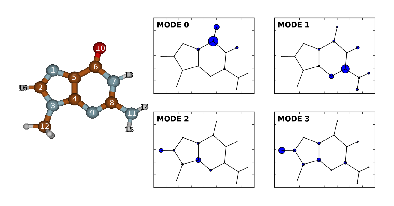
\includegraphics[width=0.9\linewidth]{guanine-1.eps}
%}
\caption{
Atomic amplitudes of selected normal modes of isolated $N$-methylguanine that were obtained by using 
TPSS-TPSS+GD3/def2-TZVP method (see Table~\ref{t:guanine-vacuum-modes}).
\label{f:guanine-vacuum-modes}}
\end{figure}
%
%
\begin{table}[t!]
\caption{
Selected normal mode frequencies of isolated $N$-methylguanine that were obtained by using 
TPSS-TPSS+GD3/def2-TZVP method. These modes are served as basis modes
for the analysis of the solvation\hyp{}induced intramolecular mode\hyp{}mixing.
\label{t:guanine-vacuum-modes}}
\begin{tabular*}{1.0\textwidth}{@{\extracolsep{\fill} } l l l l}
\hline\hline
Mode ID & Name & Frequency [cm$^{-1}$] & Relative intensity \\
\hline
0  & C$=$O stretch        & 1740  & 1.00 \\ 
1  & Ring deformation     & 1562  & 0.62 \\
2  & Ring deformation     & 1562  & 0.24 \\
3  & Ring deformation     & 1525  & 0.28 \\
\hline\hline
\end{tabular*}
\end{table}
%
The most intensive mode, C$=$O stretch (0), is also the most localised
vibration. Ring deformation modes 1 and 2 affect six\hyp{} and five\hyp{}member rings within
guanine moiety. Mode 3 deforms both rings and is the most delocalized
vibration. Since Modes 1-3 have mutual atomic overlap in
vibration amplitudes it is expected that they will tend to couple
more strongly with themselves rather than with the carbonyl stretch mode.

We have constructed thirty three $N$-methylguanine--(D$_2$O)$_{n=1-32}$ clusters.
Their description is shown in Figure~\ref{f:guanine-clusters-description}.
%
\begin{figure}[t!]
\centering
\setlength\fboxsep{0.4pt}
\setlength\fboxrule{0.5pt}
\fbox{
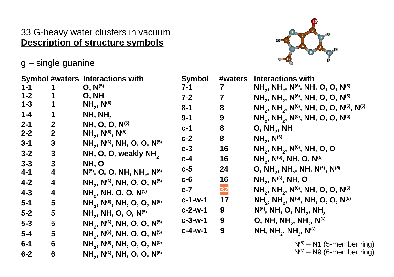
\includegraphics[width=0.9\linewidth]{guanine-2.eps}
}
\caption{
Number of solvent molecules and 
types of interactions in $N$-methylguanine--(D$_2$O)$_{n=1-32}$ that were analysed
by using TPSS-TPSS+GD3/def2-TZVP method.
\label{f:guanine-clusters-description}}
\end{figure}
%
The computed model spectral lineshapes, for which we assumed Lorenzian linewidth to be 10~cm$^{-1}$,
are shown in Figure~\ref{f:guanine-clusters-spectra}.
%
\begin{figure}[t!]
\centering
\setlength\fboxsep{0.4pt}
\setlength\fboxrule{0.5pt}
\fbox{
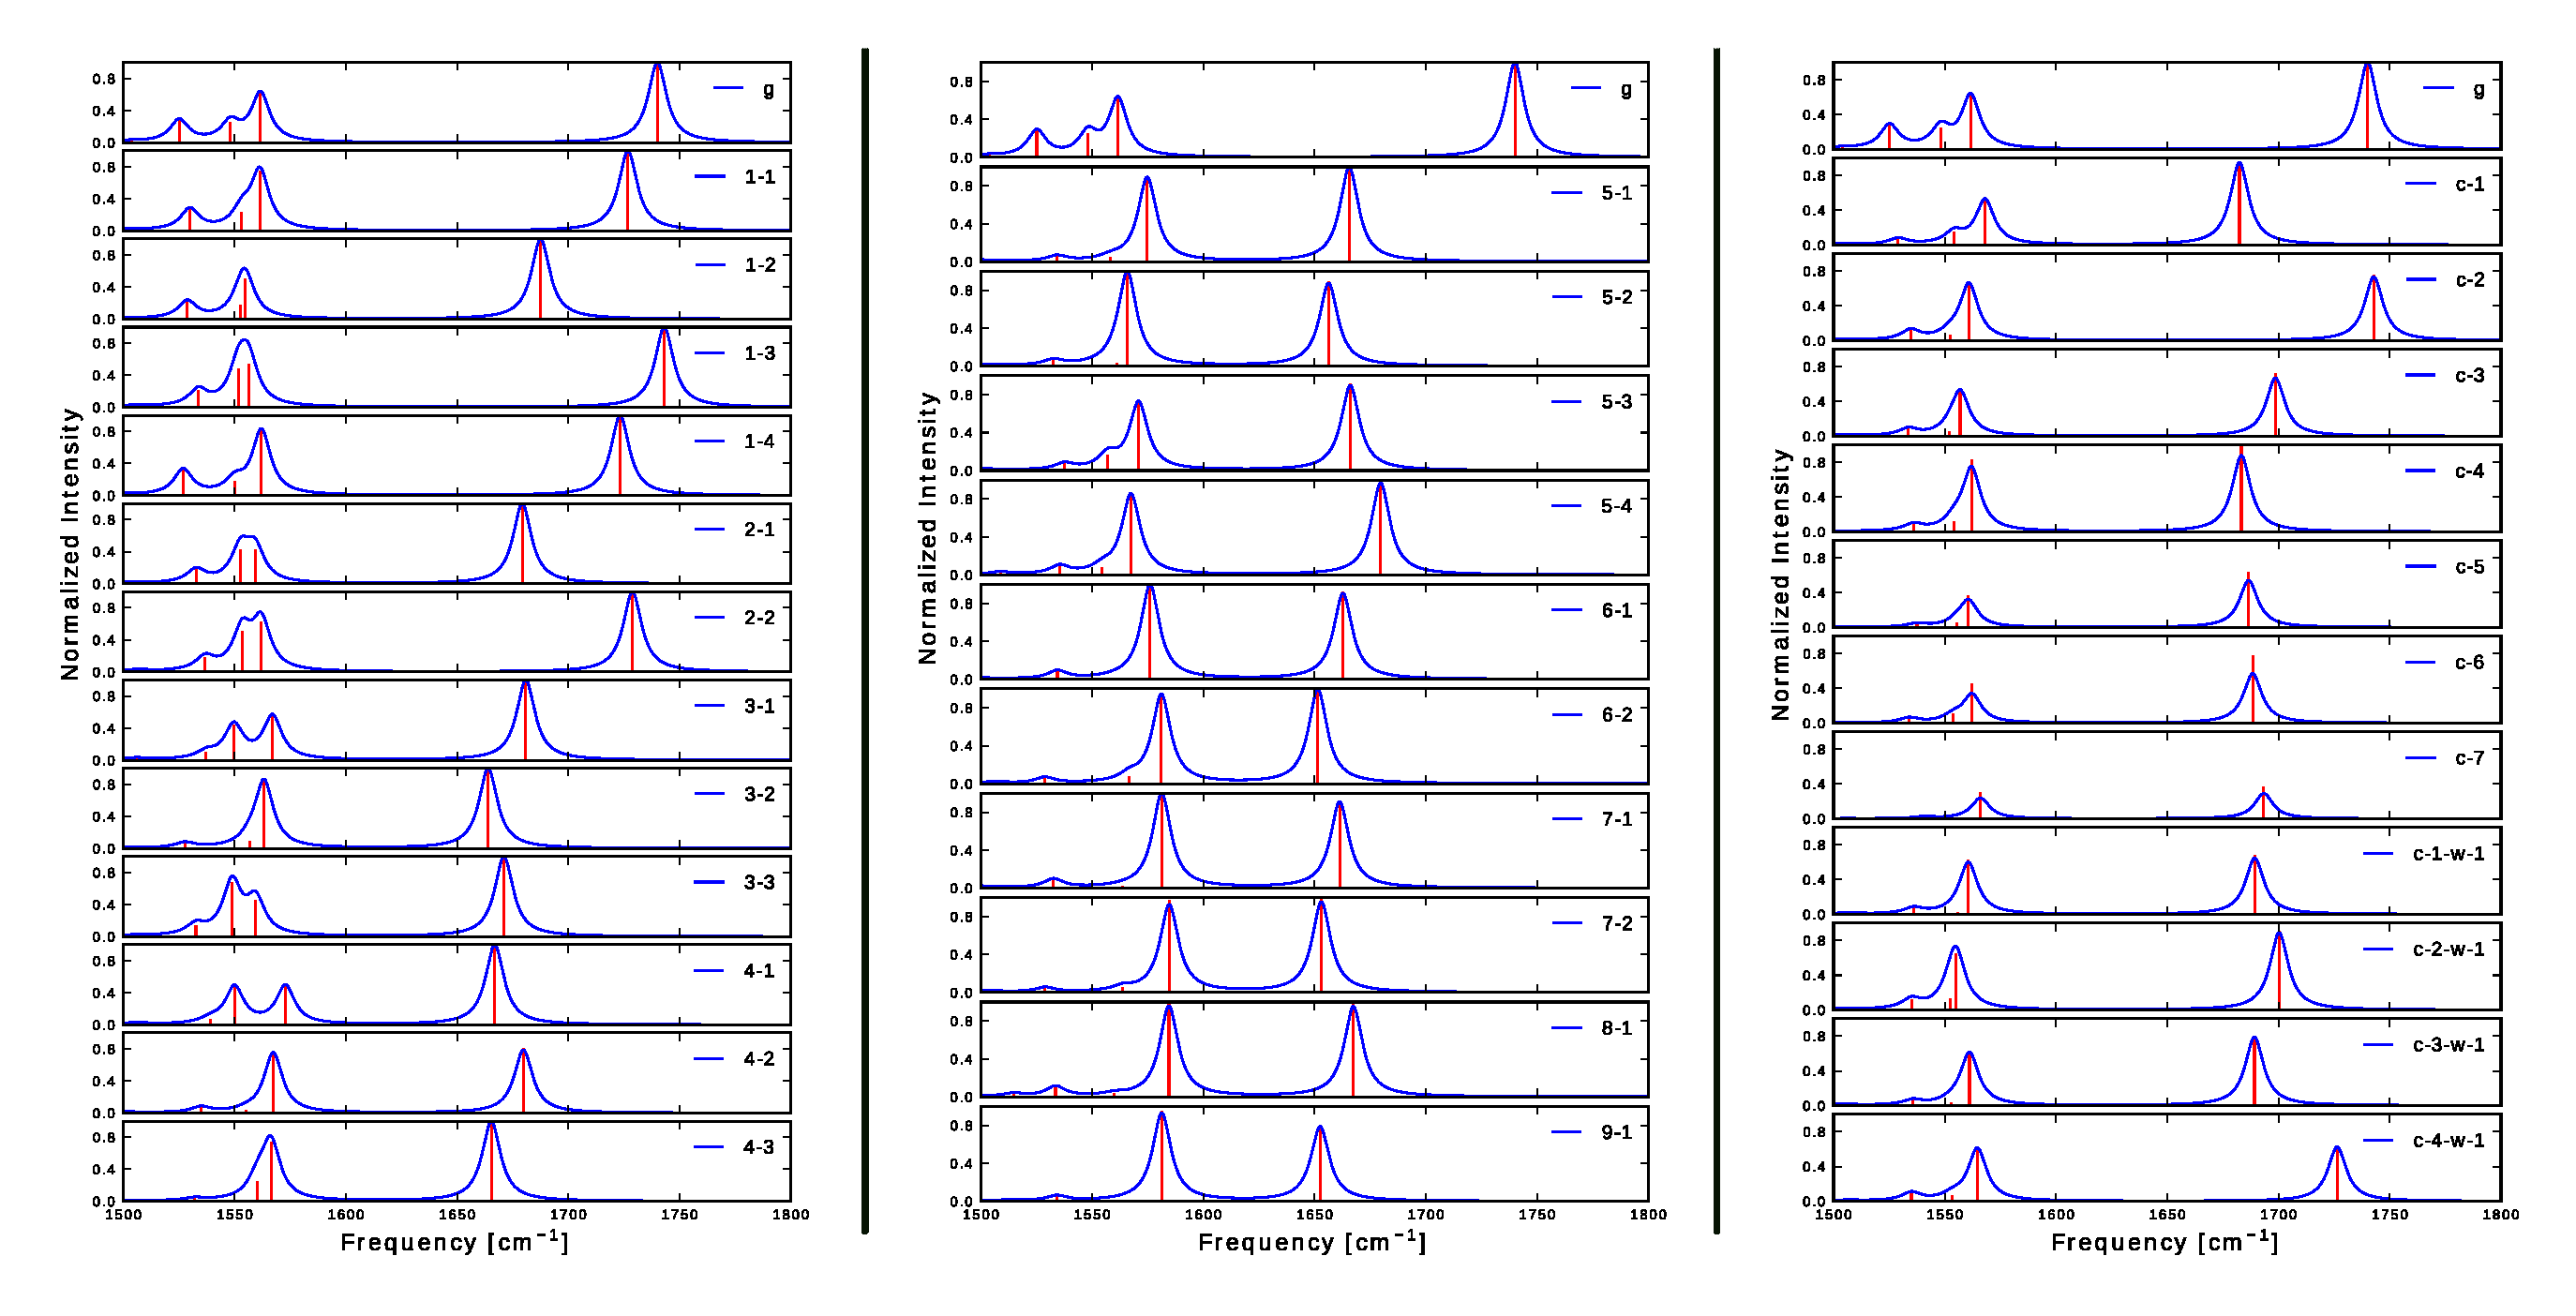
\includegraphics[width=0.97\linewidth]{123.eps}
}
\caption{
Model infrared spectra
of $N$-methylguanine--(D$_2$O)$_{n=1-32}$ clusters from 
Figure~\ref{f:guanine-clusters-description} that were analysed
by using TPSS-TPSS+GD3/def2-TZVP method. The position and height of red bars
indicate frequencies and integrated intensities, respectively. Lorenzian linewidth of 10~cm$^{-1}$
was assumed for the simulation of line shape. Spectra were normalised to
isolated $N$-methylguanine spectrum (`g' in this Figure). In each column we show
the `g' spectrum to emphasise the solvatochromic changes.
\label{f:guanine-clusters-spectra}}
\end{figure}
%
All four modes are quite sensitive to interactions with water. On the right side
of spectra we observe mostly red shifts whereas on the left side (ring modes)
blue shifts.

To investigate the nature of the normal modes of solvated guanine
more in detail we analysed their delocalization. The inverse
participation ratio, which is a measure of delocalization, 
is defined as 
%
\begin{equation}  \label{e:ipr}
 N_j = \frac{1}{\langle P_j \rangle}
\end{equation}
%
where $j$ denotes the normal mode and $P_j$
is equal to
%
\begin{equation}  
 P_j = \sum_m^{\rm atoms} \left( 
         \sum_{x \in m}^{x,y,z} \left( v^{(j)}_x \right)^2
              \right)^2
\end{equation}
%
$N_j$ is the average number of atoms over which vibration of the $j$th
mode is delocalized. Figure~\ref{f:guanine-clusters-ipr} shows $N_j$ values
plotted for each of 33 clusters. The highest frequency mode
is delocalized over 2-3 atoms and it is mostly the C$=$O stretch mode.
Ring modes however exhibit substantial degree of delocalization changes
and mode mixing is strong between them.
%
\begin{figure}[t!]
\centering
\setlength\fboxsep{0.4pt}
\setlength\fboxrule{0.5pt}
\fbox{
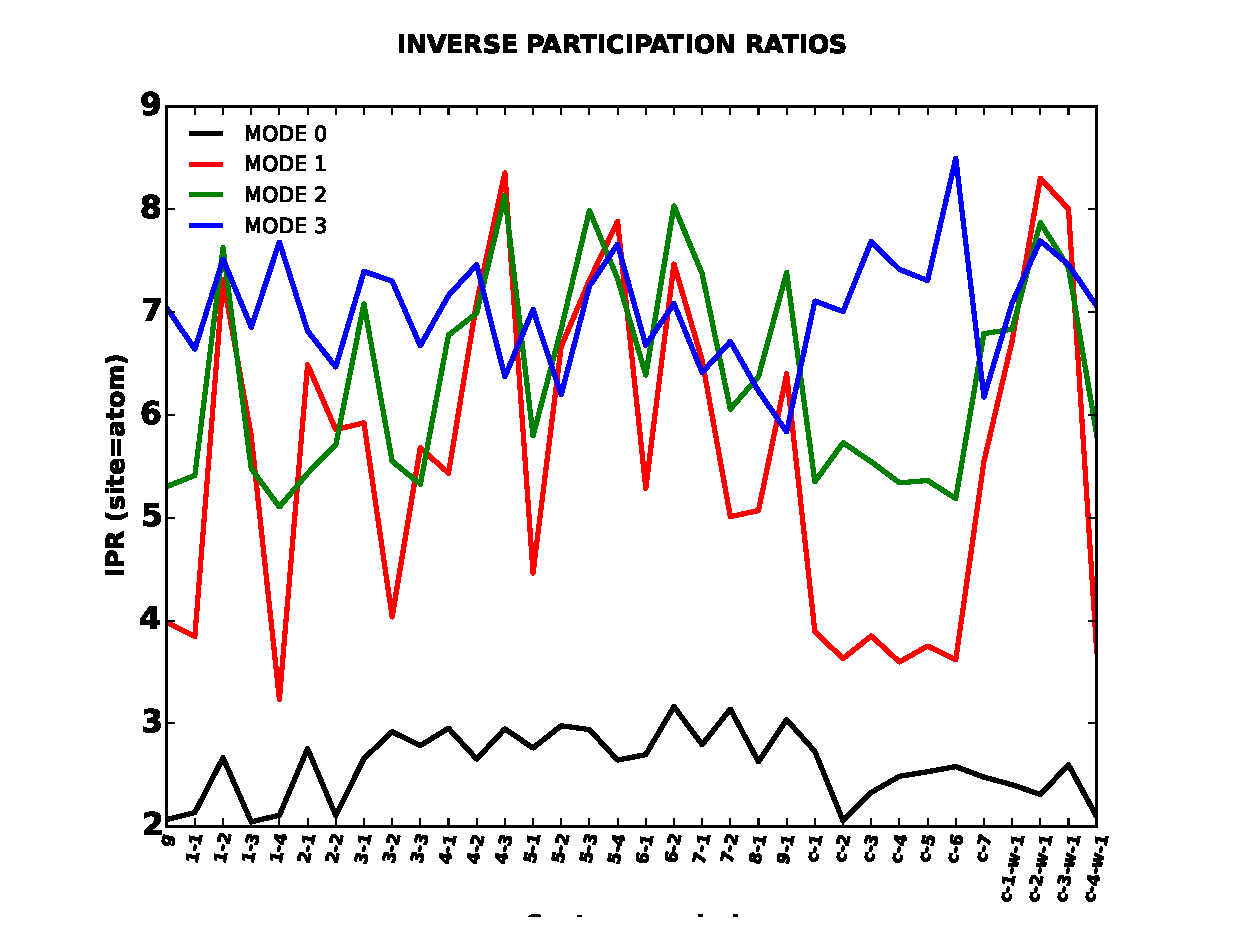
\includegraphics[width=0.97\linewidth]{ipr.eps}
}
\caption{
Inverse participation ratios $N_j$ computed for selected normal modes
for each of
$N$-methylguanine--(D$_2$O)$_{n=1-32}$ clusters from 
Figure~\ref{f:guanine-clusters-description} that were analysed
by using TPSS-TPSS+GD3/def2-TZVP method. Modes 0, 1, 2 and 3
are defined in Table~\ref{t:guanine-vacuum-modes}.
\label{f:guanine-clusters-ipr}}
\end{figure}
%

It is important to keep track of which normal mode of isolated
$N$-methylguanine become coupled with one another.
We construct the tool that helps to determine
the mode mixing between eigenvectors.
Let $S$ be the similarity function between the two
vectors ${\bf c}_1$ and ${\bf c}_2$ designed in such a way that
$S=1$ when ${\bf c}_1={\bf c}_2$ and $S=0$ when the vectors
are linearly independent (i.e., ${\bf c}_1\cdot {\bf c}_2={\bf 0}$).
This task requires adjusting properly the relative phases
of the eigenvectors from the vibrational analysis.

The simplest choice of $S$ is the following
%
\begin{equation}  
  S({\bf c}_1,{\bf c}_2) = {\bf c}_1\cdot {\bf c}_2 \sin{\phi}
\end{equation}
%
where $\phi$ is the phase factor. Such form of $S$ ensures that
vibration is periodic and we only need to adjust the relative phase
between the vibrations to maximise the dot product.
It can be done by minimising the following function
%
\begin{equation}  
  I(\phi) = \sum_i \left\{ c_{1,i} - c_{2,i} \sin{\phi}\right\}^2
\end{equation}
%
The result can be found by using the least\hyp{}squares method
and the similarity function reads
%
\begin{equation}  \label{e:similarity-function}
  S({\bf c}_1,{\bf c}_2) = \frac{ \left[{\bf c}_1\cdot {\bf c}_2 \right]^2}{{\bf c}_1\cdot {\bf c}_1}
\end{equation}
%
Figure~\ref{f:guanine-clusters-umat} shows all the similarity
matrices computed by using Eq.~\eqref{e:similarity-function}. 
Now, the mode mixing is fully revealed and
we can see clearly that ring modes become mixed in many cases. 
In particular,
modes 1 and 2 are mixed even when only one water molecule
interacts with oxygen and N--H group of $N$-methylguanine (structure
`1-2'). In contrast, mode 0 is mostly
isolated which means that C$=$O stretching motion does not flow into
low frequency motions. We speculate that WCA limit is applicable only for that
mode. Note however, that the delocalization of C$=$O stretch is not always
near the value of 2 but can reach 3 in many cases. 
%
\begin{figure}[t!]
\centering
\setlength\fboxsep{0.4pt}
\setlength\fboxrule{0.5pt}
\fbox{
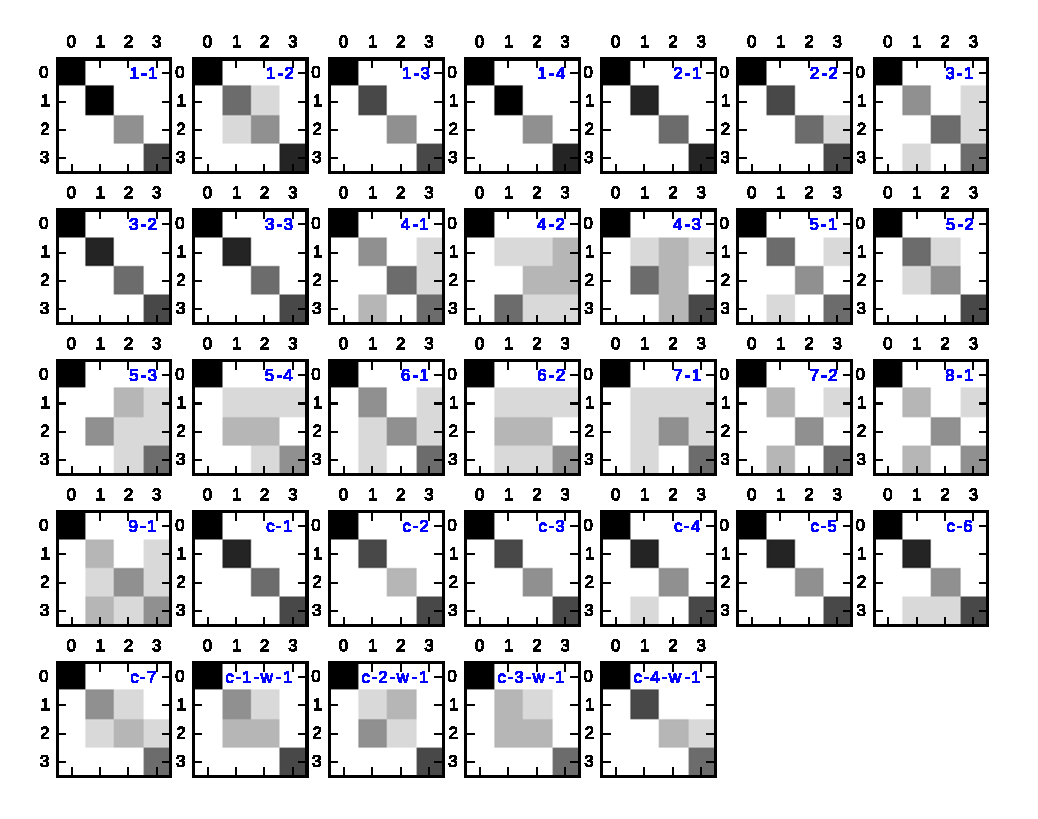
\includegraphics[width=0.94\linewidth]{u-mat.eps}
}
\caption{
Similarity matrices between selected normal modes of
$N$-methylguanine and its solvated counterparts
in $N$-methylguanine--(D$_2$O)$_{n=1-32}$ clusters from 
Figure~\ref{f:guanine-clusters-description} that were analysed
by using TPSS-TPSS+GD3/def2-TZVP method. Modes 0, 1, 2 and 3
are defined in Table~\ref{t:guanine-vacuum-modes}.
In this Figure, horizontal and vertical axes denote $N$-methylguanine's
normal modes in vacuum
and in (D$_2$O)$_{n=1-32}$ cluster, respectively.
\label{f:guanine-clusters-umat}}
\end{figure}
%
This can be understood 
by analysing the atomic vibration amplitude maps shown
for $N$-methylguanine in each each cluster
that is shown in Figure~\ref{f:guanine-clusters-amplitudes}.
Mode 0 often
involves also other atoms within 6-member ring as can be seen, for example,
for structures in a range from `3-2' to `9-1'. From that figure
the mode mixing between ring vibrations is also qualitatively
apparent and can be relatively easily tracked.
%
\begin{figure}[t!]
\centering
\setlength\fboxsep{0.4pt}
\setlength\fboxrule{0.5pt}
\fbox{
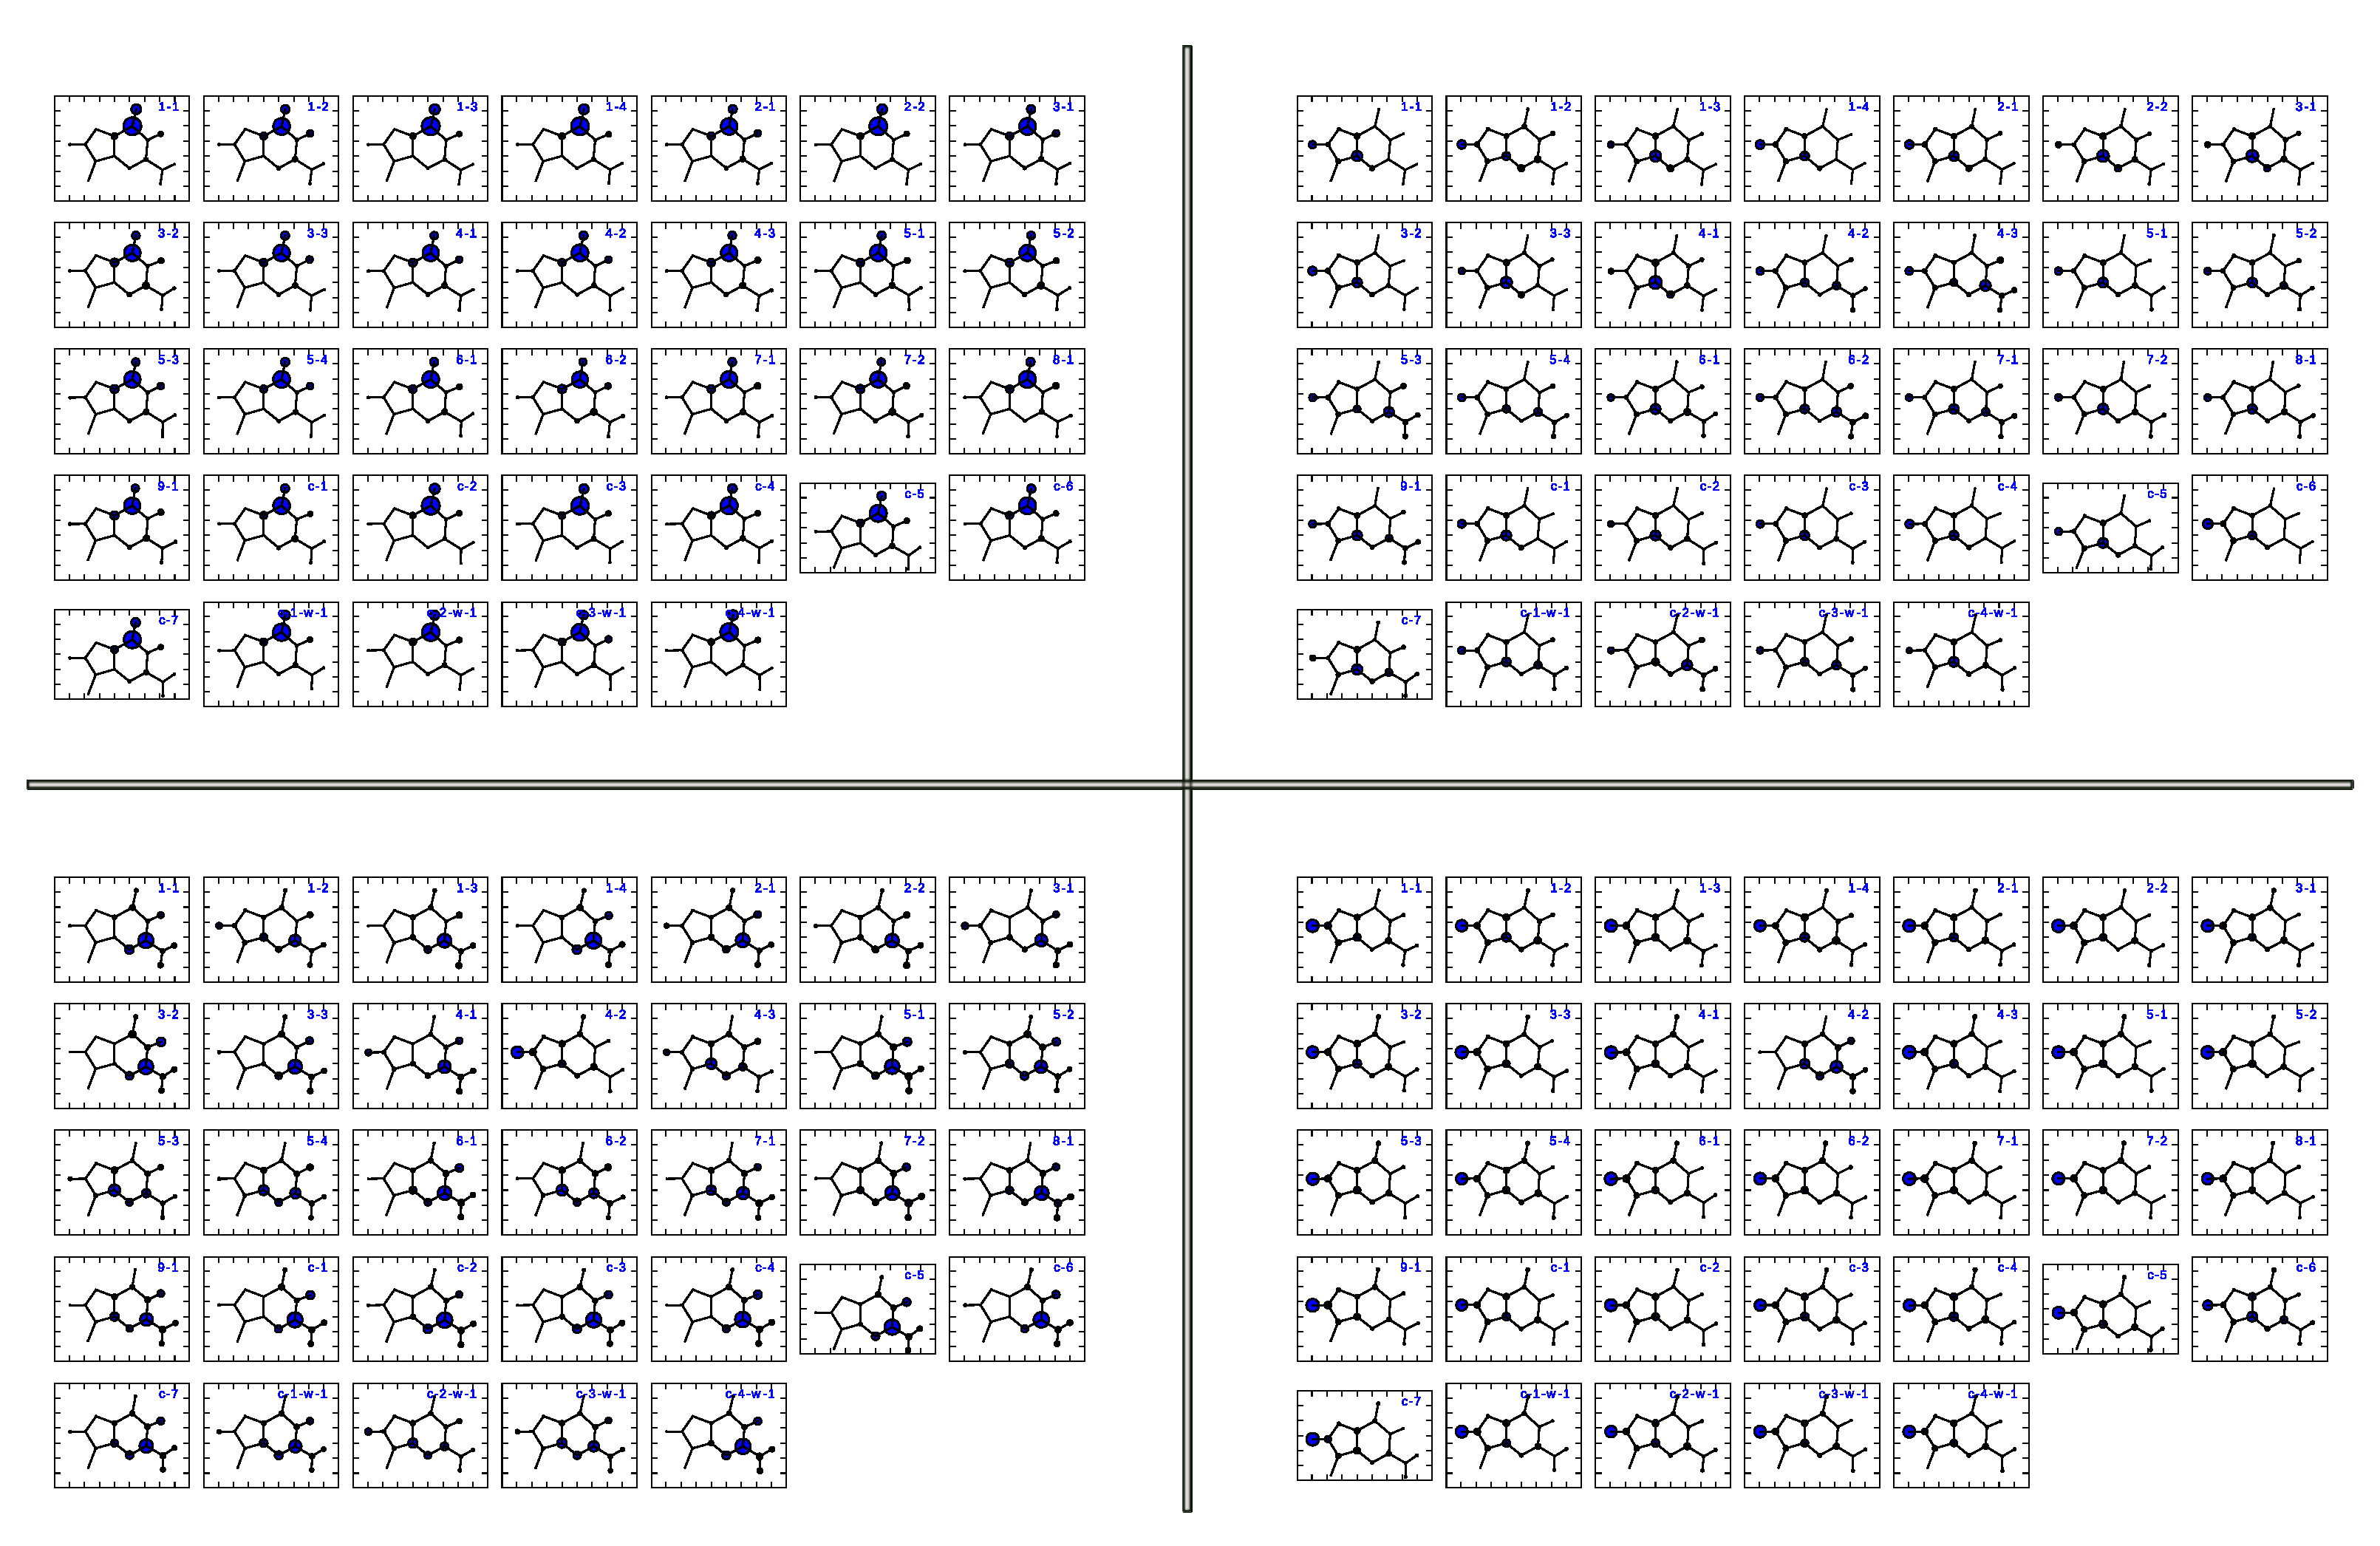
\includegraphics[width=0.98\linewidth]{mol.amplitudes.eps}
}
\caption{
Atomic vibration amplitudes for selected normal modes of
$N$-methylguanine
in $N$-methylguanine--(D$_2$O)$_{n=1-32}$ clusters from 
Figure~\ref{f:guanine-clusters-description} that were analysed
by using TPSS-TPSS+GD3/def2-TZVP method. For comparison, the vacuum atomic amplitudes
are shown in the insets at the bottom right corners of each plot.
\label{f:guanine-clusters-amplitudes}}
\end{figure}
%

The effects of water molecules on the mode mixing
within guanine rings are summarised in Figure~\ref{f:guanine-clusters-summary}.
%
\begin{figure}[t!]
\centering
\setlength\fboxsep{0.4pt}
\setlength\fboxrule{0.5pt}
\fbox{
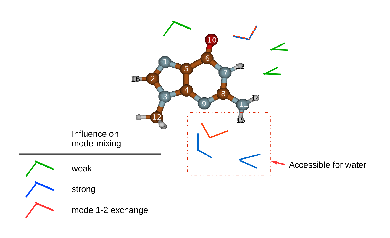
\includegraphics[width=0.97\linewidth]{guanine-3.eps}
}
\caption{
Effects of water H-bonding to various accepting sites
of $N$-methylguanine on its interaction\hyp{}induced mode mixing.
The region indicated in red box refers to the situation
when $N$-methylguanine is forming a G-quadruplex structure. \citep{Peng.Jones.Tokmakoff.JACS.2011}
\label{f:guanine-clusters-summary}}
\end{figure}
%
It is seen that the the interactions of water with easily accessible sites (when guanine
forms nucleic acid or G-quadruplex \citep{Peng.Jones.Tokmakoff.JACS.2011}) 
can induce strong mixing.
This is particularly important when one wants to use model that
is based on isolated nucleobases. Indeed, in such a case WCA
limit cannot be accepted at all for ring modes and one needs to consider
solute's Hessian matrix in more detail.

\section{Summary}

In this Chapter we discussed the solvation\hyp{}induced
intramolecular mode mixing which is a difficult problem
when modelling the IR spectra for nucleic acids based on
isolated nucleobases. The first\hyp{}principles theory
of the vibrational solvatochromism beyond WCA should be studied
in the future. More specifically, one could evaluate
the new eigenvectors and compute similarity matrices
which are to be compared with similarity matrices from
Figure~\ref{f:guanine-clusters-umat}. This work is in progress.





\printbibliography[heading=subbibintoc,title={References}]
\end{refsection}



% ------------------- CHAPTER 8 ------------------------

\begin{refsection}
\chapter{The Solvshift Program\label{c:slv}}

In this part of the Thesis, we briefly present the {\sc Solvshift}
package. The basic concept behind it is to develop the fragment\hyp{}based
approach to calculation of the solvation or interaction induced
molecular properties such as changes in vibrational frequency and vibrational 
transition dipole, nonlinear optical properties, magnetic shielding
constants or electronic energy levels. Here, we focus on the
vibrational property calculations using {\sc Solvshift}.

\section{Overview}

{\sc Solvshift} (SLV) is a further development of {\sc Coulomb} package
that is designed for calculations of electrostatic properties of molecules
by means of quantum chemistry methods and it has been developed
since 2010. Originally, written in pure Python, {\sc Coulomb} utilised
the so called Gaussian Lobe Orbitals (GLO) introduced in early quantum chemistry
times by Whitten in 1960s. \citep{Whitten.JCP.1966,Whitten.JCP.1969} 
GLO imitate the GTFs by linear combinations
of $s$-type functions so that the computational procedure of solving
Hartree\hyp{}Fock or Kohn\hyp{}Sham equations are relatively simple
in implementation. In early form of {\sc Coulomb}, the integral package, i.e.,
the module that manages the evaluation of the one\hyp{}electron overlap (SI), multipole (MI),
kinetic (KI) and
potential (VI) integrals as well as the two\hyp{}electron
repulsion integrals (ERI) was implemented in a straightforward way
so that the performance of the code was quite limited to small molecules
and small basis sets (the largest molecule studied by GLO\hyp{}Python version
was acetic acid in a basis which is comparable to 6-31G(p) with additional polarization
$p$ functions imitating $d$-orbitals on carbon and oxygen atoms). Nevertheless,
the code was able to compute basic electrostatic molecular properties such as
molecular multipole moments and cumulative atomic multipole moments 
(CAMM's) \citep{Sokalski.Poirier.CPL.1983} up to octupoles.
 
In 2011 {\sc Coulomb} was upgraded and coupled with the two codes to shift to GTF\hyp{}based
basis sets up to $g$-functions and increase its efficiency:
%
\begin{itemize}
\item {\sc PyQuante} -- Python implementation of LCAO-MO method by Richard Muller \citep{Muller.PyQuante.2009}
\item {\sc LibInt} -- Highly efficient integral package by Edward Valeev \citep{Valeev.LibInt.2013}
\item {\sc Gaussian 09} -- High\hyp{}performance quantum chemistry suite of programs \citep{Frisch.Gaussian.2009}
\end{itemize}
%
The coupling with {\sc Gaussian 09} \citep{Frisch.Gaussian.2009} 
enabled reading the one\hyp{}particle 
density matrices (and transition density matrices in case of excited state
calculations) based on which electrostatic calculations could be performed
for methods not implemented (or quite slow) in {\sc Coulomb} such as the 
configuration interaction theory (CI), the
coupled\hyp{}cluster theory (CC) or the density functional theory (DFT).
In particular, {\sc Coulomb} was able to compute the exact first\hyp{}order
Coulombic interaction energy (including charge\hyp{}penetration),
and the associated exchange\hyp{}repulsion correction to account
for the antisymmetric nature of electronic wavefunctions.
Also, the
approximate Coulombic interaction energy derived from CAMM or DMA
was also available.

Since 2012, we were developing the code to manage effective fragment
potentials (EFP) for induction, exchange\hyp{}repulsion and dispersion
effects. As a result, {\sc Solvshift} package was introduced
to manage the EFP\hyp{}based approaches in the calculations
of the vibrational frequency shifts and so on. As for now, 
the functionalities of the code are as follows
%
\begin{itemize}
 \item {\sc Coulomb}
  \begin{itemize}
  \item Computing CAMM and MMM at arbitrary origin
  \item Management of CAMM/DMA distributions: rotations, translations, recentering of origins
  \item Calculation of exact first\hyp{}order 
        electrostatic and exchange\hyp{}repulsion interaction energy for a dimer
  \item Calculation of multiple expansion\hyp{}derived interaction energy
  \item Coupling with {\sc Gaussian 09}: reading one\hyp{}particle 
                                        density matrices
  \item Computation of transition cumulative atomic multipole moments (TrCAMM)
        and excitonic energy transfer (EET) couplings \citep{Blasiak.Maj.Cho.Gora.JCTC.2015}
  \end{itemize}
 \item {\sc Solvshift}
  \begin{itemize}
  \item Computing EFP Coulombic, induction, dispersion, exchange\hyp{}repulsion and approximate CT
        interaction potential
  \item Computing SolEFP frequency shifts and transition dipole moment change:
        i) Coulombic term under mechanical and electric anharmonicity, 
        ii) induction, dispersion and exchange\hyp{}repulsion terms under mechanical anharmonicity
  \item Onsager model of solvation: rigid and flexible models
  \item Rigid molecule algorithm for Coulomb, induction, dispersion and exchange\hyp{}repulsion
        parameters
  \item Management of classical molecular dynamics trajectory files from Gromacs, Amber and NAMD
  \item Implementation of EFP fragmentation model for protein environment within SolEFP model
  \end{itemize}
\end{itemize}
%
In the following Sections, we describe the structure, main classes,
usage examples and future development of the {\sc Solvshift} code.

\section{Idea of Solvshift}

SLV program implements mostly all of the equations that were derived
and presented in this Thesis. 
The principle of operation of SLV depends on the SolX method chosen:
%
\begin{itemize}
  \item Run by using {\bf Constrained cluster algorithm (CCA)}:
        SolEDS, SolSAPT and SolEFP\footnote{evaluation of vibrational derivatives numerically} 
        methods (Section~\ref{s:solefp-soleds-solsapt}). The vibrational derivatives of interaction
        energies are evaluated numerically through interface with EDS code
        written by my previous Supervisor Robert W. G{\'o}ra \citep{Gora.EDS.1998-2010}
        or EFP2 method implemented in {\sc GAMESS}~CITATION.
  \item Run by using {\bf Rigid molecule algorithm (RMA)}:
        SolCAMM, SolDMA, SolChelpG, SolLMTP, SolMMM and SolEFP methods (Section~\ref{s:solx-electrost}).
        The vibrational derivatives are evaluated by using analytical approximate formulae.
\end{itemize}
%
The CCA method is designed for analysis of small model systems
and can serve also as a validation tool for methods based on RMA
since no multipole expansion is introduced and the frequency shift
components are evaluated without additional approximations.

However, for the analysis of large systems RMA needs 
to be utilised. In this case, the solvatochromic model is constructed 
from the independent benchmark molecule parameters (IBM's)
which are the representations of the isolated molecules in their gas\hyp{}phase states.
These parameters serve as \emph{ab initio} templates to be superimposed later onto
the target system and they are computed once and for all.
In Table~\ref{t:slv-rma-parameters}
we present the list of such parameters that
build IBM's. In the case of solvent molecule,
IBM is equivalent to the conventional EFP2 parameters.\footnote{with 
CAMM's instead of distributed multipole analysis moments
(DMA's) of Stone \citep{Stone.JCTC.2005} in the current implementation}
%
\begin{table}[t!]
\caption{
 Parameters of independent benchmark molecule (IBM's) used in SLV code grouped
 into four main categories: Molecule specification (I.), Electrostatic population
 parameters (II.), Frequency analysis (III.) and Wavefunction and electronic structure (IV.).
 Abbreviations for symbols: $N$ - number of atoms, $D$ - number of distributed multipole centres,
 $M$ - number of normal modes, $M'$ - number of normal modes for which diagonal derivatives
 are to be computed, $P$ - number of polarizable centres, $n$ - number of localised (occupied) molecular
 orbitals (LMO's), $c$ - number of canonical (occupied and virtual) molecular orbitals (CMO's) which is equal to
 number of basis functions $\beta$, $a$ and $b$ - labels for LMO's, $x$ - label for atomic centre, 
 $X$ - label for molecule.
\label{t:slv-rma-parameters}}
\begin{tabular*}{1.0\textwidth}{@{\extracolsep{\fill} } lllll}
\hline\hline
%\multicolumn{5}{c}{Amide I mode} \\
 Category   & Parameter & Label & Symbol$^{a)}$ & Dimension \\
\hline
\multirow{3}{*}{I.}
&Atomic numbers                         &\tt{atno    } &   $Z_x$                                     &      $N$                                 \\                                        
&Atomic masses                          &\tt{atms    } &   $m_x$                                     &      $N$                                 \\
&Atomic coordinates                     &\tt{pos     } &   ${\bf r}_x$                               &      $N\times 3$                         \\
% - - - - - - - - - - - - - - - - - - - - - - - - - - - - - - - - - - - - - - - - - - - - - - - - - - - - - - - - - - - - - - - - - - 
\hline                                                                                                   
\multirow{20}{*}{II.}                                                                                    
&ESP charges                            &\tt{esp     } &   $q_x$                                     &      $N$                                 \\
&ChelpG charges                         &\tt{chlpg   } &   $q_x$                                     &      $N$                                 \\
&DMTP centers                           &\tt{rdma    } &   ${\bf r}_x$                               &      $D\times 3$                         \\    
&DMTP charges                           &\tt{dmac    } &   $q_x$                                     &      $D$                                 \\
&\textbullet 1$^{\rm st}$ derivatives   &\tt{dmac1   } &   $\fderivm{q_x}{Q_i}$                      &      $M\times D$                         \\
&\textbullet 2$^{\rm nd}$ derivatives   &\tt{dmac2   } &   $\sderivm{q_x}{Q_j}$                      &      $M'\times D$                        \\                                           
&DMTP dipoles                           &\tt{dmad    } &   ${\BM\upmu}_x$                            &      $D\times 3$                         \\  
&\textbullet 1$^{\rm st}$ derivatives   &\tt{dmad1   } &   $\fderivm{{\BM\upmu}_x}{Q_i}$             &      $M\times D\times 3$                 \\    
&\textbullet 2$^{\rm nd}$ derivatives   &\tt{dmad2   } &   $\sderivm{{\BM\upmu}_x}{Q_j}$             &      $M'\times D\times 3$                \\
&DMTP quadrupoles                       &\tt{dmaq    } &   ${\BM\Theta}_x$                           &      $D\times 6$                         \\ 
&\textbullet 1$^{\rm st}$ derivatives   &\tt{dmaq1   } &   $\fderivm{{\BM\Theta}_x}{Q_i}$            &      $M\times D\times 6$                 \\   
&\textbullet 2$^{\rm nd}$ derivatives   &\tt{dmad2   } &   $\sderivm{{\BM\Theta}_x}{Q_j}$            &      $M'\times D\times 6$                \\
&DMTP octupoles                         &\tt{dmao    } &   ${\BM\Omega}_x$                           &      $D\times 10$                        \\
&\textbullet 1$^{\rm st}$ derivatives   &\tt{dmao1   } &   $\fderivm{{\BM\Omega}_x}{Q_i}$            &      $M\times D\times 10$                \\  
&\textbullet 2$^{\rm nd}$ derivatives   &\tt{dmao2   } &   $\sderivm{{\BM\Omega}_x}{Q_j}$            &      $M'\times D\times 10$               \\
&Polarizable centers                    &\tt{rpol    } &   ${\bf r}_a$                               &      $P\times 3$                         \\
&Distributed polarizabilities           &\tt{dpol    } &   ${\BM\alpha}_a(0)$                        &      $P\times 9$                         \\      
&\textbullet 1$^{\rm st}$ derivatives   &\tt{dpol1   } &   $\fderivm{{\BM\alpha}_a(0)}{Q_i}$         &      $M\times P\times 9$                 \\                                          
&Dist. pol. wrt imaginary freq          &\tt{dpoli   } &   ${\BM\alpha}_a(i\Omega)$                  &      $P\times 12\times 9$                \\
&\textbullet 1$^{\rm st}$ derivatives   &\tt{dpoli1  } &   $\fderivm{{\BM\alpha}_a(i\Omega)}{Q_i}$   &      $M\times P\times 12\times 9$        \\
% - - - - - - - - - - - - - - - - - - - - - - - - - - - - - - - - - - - - - - - - - - - - - - - - - - - - - - - - - - - - - - - - - - 
\hline                                                                                            
\multirow{4}{*}{III.}                                                                             
&Harmonic frequencies                   &\tt{freq    } &   $\omega_i$                                &      $M$                                 \\ 
&Reduced masses                         &\tt{redmass } &   $M_i$                                     &      $M$                                 \\
&Vibrational eigenvectors             &\tt{lvec    } &   ${\bf L}^{(i)}_x$                         &      $M\times N\times 3$                 \\
&Cubic anharmonic constants             &\tt{gijk    } &   $g_{ijk}$                                 &      $M\times M\times M$                 \\
% - - - - - - - - - - - - - - - - - - - - - - - - - - - - - - - - - - - - - - - - - - - - - - - - - - - - - - - - - - - - - - - - - - 
\hline                                                                                            
\multirow{10}{*}{IV.}                                                                             
&LMO centroids                          &\tt{lmoc    } &   ${\bf r}_a$                               &      $n\times 3$                         \\                                                 
&\textbullet 1$^{\rm st}$ derivatives   &\tt{lmoc1   } &   $\fderivm{{\bf r}_x}{Q_i}$                &      $M\times n\times 3$                 \\                                              
&Fock matrix                            &\tt{fock    } &   $G^{\rm X}_{ab}$                          &      $n\times n$                         \\
&\textbullet 1$^{\rm st}$ derivatives   &\tt{fock1   } &   $\fderivm{G^{\rm X}_{ab}}{Q_i}$           &      $M\times n\times n$                 \\                                             
&Canonical Fock matrix                  &\tt{fckc    } &   $G^{\rm X}_{\alpha\beta}$                 &      $c\times c$                         \\
&\textbullet 1$^{\rm st}$ derivatives   &\tt{fckc1   } &   $\fderivm{G^{\rm X}_{\alpha\beta}}{Q_i}$  &      $M\times c\times c$                 \\    
&LCAO-LMO matrix                        &\tt{vecl    } &   $C_{a\alpha}$                             &      $n\times \beta$                     \\       
&\textbullet 1$^{\rm st}$ derivatives   &\tt{vecl1   } &   $\fderivm{C_{a\alpha}}{Q_i}$              &      $M\times n\times \beta$             \\                                             
&LCAO-CMO matrix                        &\tt{vecc    } &   $C_{a\alpha}$                             &      $c\times \beta$                     \\
&\textbullet 1$^{\rm st}$ derivatives   &\tt{vecc1   } &   $\fderivm{C_{a\alpha}}{Q_i}$              &      $M\times c\times \beta$             \\                                                
\hline\hline
\end{tabular*}
%
\begin{footnotesize}
$^{a)}$ Mathematical symbols which are used throughout the Thesis.
\end{footnotesize}
\end{table}
%
In the case of IR active molecules additionally first and second
derivatives with respect to normal coordinates as well as
harmonic and anharmonic vibrational analysis parameters
need to be computed. As can be seen, the amount of data per one IBM is quite
substantial with exchange\hyp{}repulsion parameters constituting of mostly 90\% 
of all parameters. This is because the basis sets for EFP2 calculations
should be of at least 6-31++G** quality.
For instance, in the case of MeSCN and 6-311++G** basis set, 
the amount of Fock matrix elements in LMO basis
and its first derivatives
is 190 and 2850, respectively,
whereas the amount of LCAO-MO wavefunction coefficients and their derivatives
hits as far as accordingly 2299 and 34485 numbers!
Despite all this, the present implementation handles IBM's parameters
efficiently and the associated net computer usage while reading, writing
or processing the parameters
can be considered as negligible.

SLV has already decent set of built-in parameters computed 
by using 6-311++G** basis set. The currently implemented IBM's
are shown in Table~\ref{t:slv-ibm-buitin}
%
\begin{table}[t!]
\caption{
Built-in independent benchmark molecule parameters that are implemented
in the current version of {\sc Solvshift}. Abbreviations: ``EINT'' - interaction
energy, ``FREQ'' - vibrational properties.
\label{t:slv-ibm-buitin}}
\begin{tabular*}{1.0\textwidth}{@{\extracolsep{\fill} } lllll}
\hline\hline
 SLV Label             & Molecule                        & EINT &   FREQ   &     Comment                              \\
\multicolumn{5}{c}{SolEFP parameters} \\                                                           
\hline                                                                      
 \tt{meoac           } & Methyl acetate                  & YES  &   YES    &     C$=$O stretch                        \\ 
 \tt{nma             } & $N$-Methyl Acetamide            & YES  &   YES    &     amide I mode                         \\
 \tt{nma-d7          } & NMA$_{d_7}$ $^{a)}$             & YES  &   YES    &     amide I' mode                        \\
 \tt{mescn           } & Methyl Thiocyanide              & YES  &   YES    &     C$\equiv$N stretch                   \\
 \tt{mecn            } & Methyl Nitrile                  & YES  &   YES    &     C$\equiv$N stretch                   \\
 \tt{et2coo          } & Diethyl Carbonate               & YES  &   YES    &     C$=$O stretch                        \\
\multicolumn{5}{c}{EFP parameters} \\                                                                                   
\hline                                                                                                                  
 \tt{water           } & H$_2$O                          & YES  &   NO     &     with DMA-5                           \\
 \tt{water2          } & H$_2$O                          & YES  &   NO     &     with CAMM-3                          \\
 \tt{dmso            } & DMSO                            & YES  &   NO     &                                          \\
 \tt{meoh            } & Methanol                        & YES  &   NO     &                                          \\
 \tt{etoh            } & Ethanol                         & YES  &   NO     &                                          \\
 \tt{mesh            } & Methanothiol                    & YES  &   NO     &                                          \\
 \tt{dms             } & Dimethylsylfide                 & YES  &   NO     &                                          \\
 \tt{menh2           } & Methylamine                     & YES  &   NO     &                                          \\
 \tt{ccl4            } & Tetrachloromethane              & YES  &   NO     &                                          \\
 \tt{chcl3           } & Chloroform                      & YES  &   NO     &                                          \\
 \tt{dcm             } & Dichloromethane                 & YES  &   NO     &                                          \\
 \tt{li+             } & Lithium Cation                  & YES  &   NO     &                                          \\
 \tt{na+             } & Sodium Cation                   & YES  &   NO     &                                          \\
 \tt{me-so3-         } & Methyl Sulphonate (-1)          & YES  &   NO     &                                          \\
 \tt{so3--           } & SO$_3^{2-}$ anion               & YES  &   NO     &                                          \\
 \tt{imidazole       } & Imidazole                       & YES  &   NO     &                                          \\
 \tt{4-me-imidazole  } & 4-Methyl Imidazole              & YES  &   NO     &                                          \\
 \tt{4-me-phenol     } & 4-Methyl Phenol                 & YES  &   NO     &                                          \\
 \tt{chonh2          } & Formamide                       & YES  &   NO     &                                          \\
 \tt{chonhme         } & N-Methyl Formamide              & YES  &   NO     &                                          \\
 \tt{comenh2         } & Acetamide                       & YES  &   NO     &                                          \\
 \tt{mecoo-          } & Acetate (-1) Anion              & YES  &   NO     &                                          \\
 \tt{menh3+          } & Methyl Ammonium (+1) Cation     & YES  &   NO     &                                          \\
 \tt{me-guanidinium+ } & Methyl Guanidinium (+1) Cation  & YES  &   NO     &                                          \\
 \tt{methane         } & Methane                         & YES  &   NO     &                                          \\
 \tt{ethane          } & Ethane                          & YES  &   NO     &                                          \\
 \tt{n-propane       } & $n$-Propane                     & YES  &   NO     &                                          \\
 \tt{cyclohexane     } & Cyclohexane                     & YES  &   NO     &                                          \\
 \tt{benzene         } & Benzene                         & YES  &   NO     &                                          \\
 \tt{phenole         } & Phenole                         & YES  &   NO     &                                          \\
 \tt{dmf             } & Dimethylformamide               & YES  &   NO     &                                          \\
 \tt{thf             } & Tetrahydrofurane                & YES  &   NO     &                                          \\
 \tt{cho-ch-nh2-ch3  } & 2-Aminopropanal                 & YES  &   NO     &                                          \\
\hline\hline
\end{tabular*}
%
\begin{footnotesize}
$^{a)}$ all H deuterated.
\end{footnotesize}
\end{table}
%



\section{Structure of Solvshift}

Figure~\ref{f:slv-solefp} shows the outline of the overall procedure 
of applying RMA\hyp{}based methods that are implemented in the SLV program.
%
\begin{figure}[t!]
\centering
\setlength\fboxsep{0.4pt}
\setlength\fboxrule{0.5pt}
%\fbox{
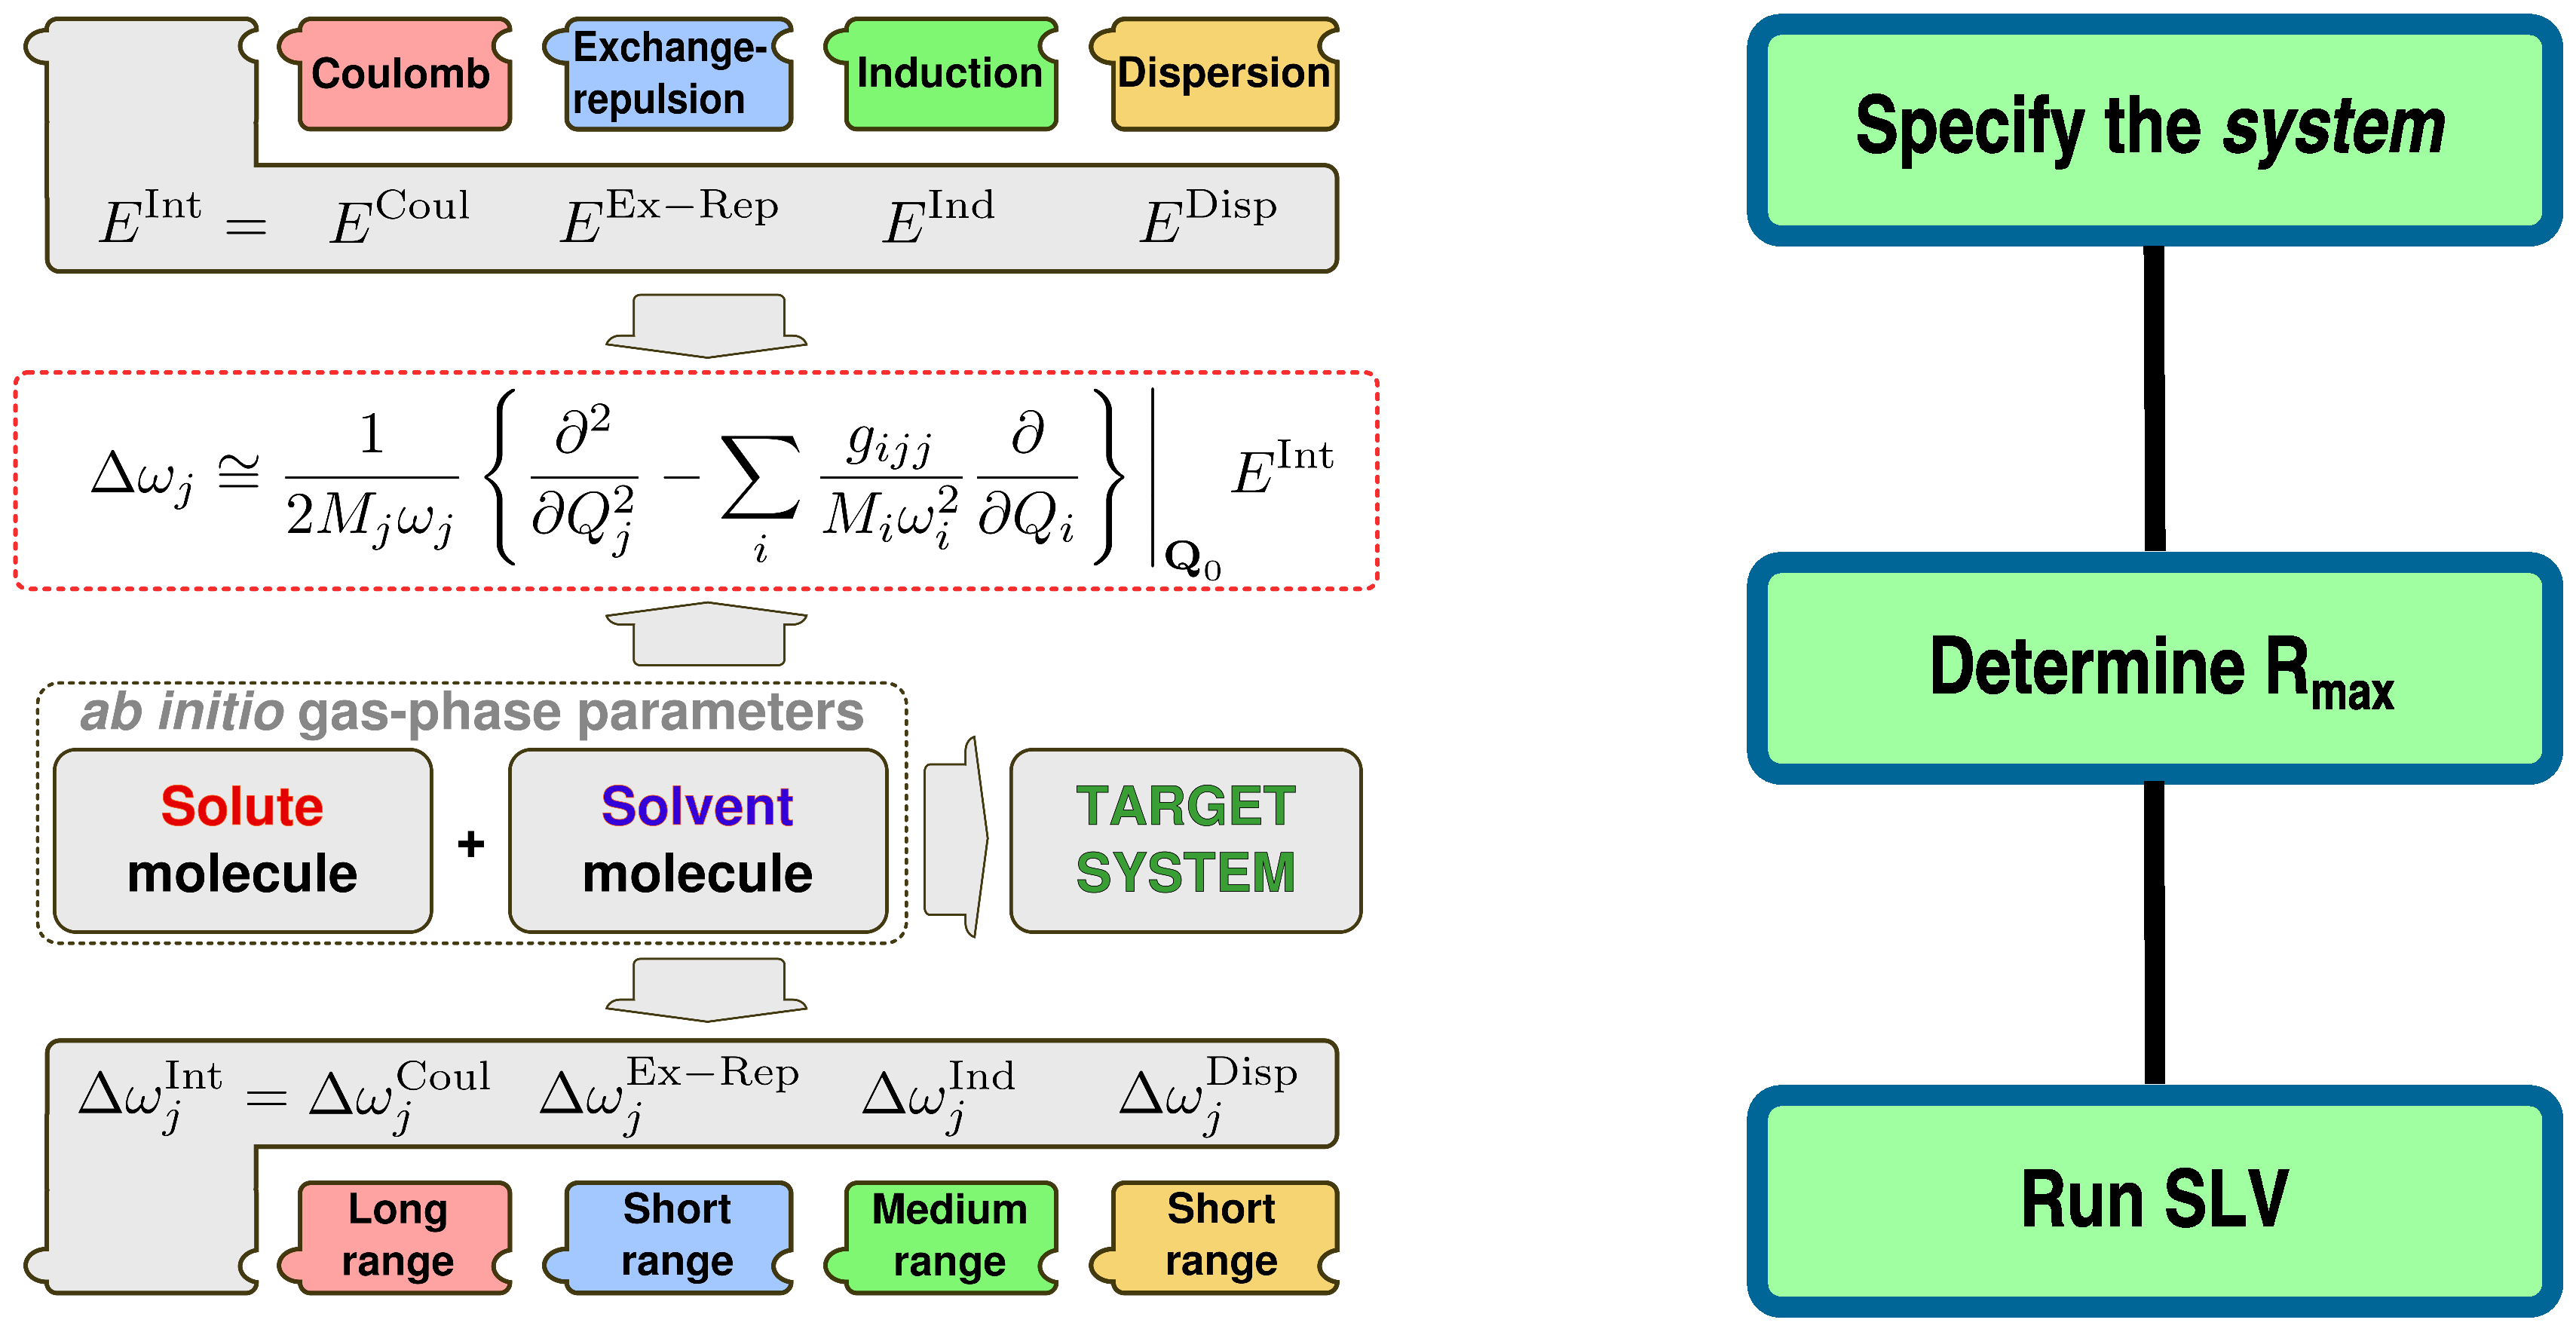
\includegraphics[width=0.92\linewidth]{slv-fig-2.eps}
%}
\caption{
\emph{Left:} Evaluation of vibrational property by using SolX methods based 
             on the rigid molecule algorithm.
\emph{Right:} Applying SolX models to molecular systems.
\label{f:slv-solefp}}
\end{figure}
%
The most time\hyp{}consuming part of SLV RMA run is the computation
of vibrational displacements $\delta Q_i$ due to each intermolecular
interaction potential. These displacements are then used to compute the
solvation\hyp{}induced vibrational frequency shifts 
and the transition dipole moment changes with negligible computational effort.
Therefore, development should be undertaken to improve the
performance of the $\delta Q_i$ evaluation, especially 
$\delta Q_i^{\rm Ind}$, $\delta Q_i^{\rm Ex-Rep}$
and $\delta Q_i^{\rm CT}$. Yet another heavy quantity is
the distributed solvatochromic induced dipole moments ${\bf a}_j$.
Their computation is not necessary but may be useful in some cases.

The basic structure of {\sc Solvshift} is shown
in Figure~\ref{f:slv-structure}.
%
\begin{figure}[t!]
\centering
\setlength\fboxsep{0.4pt}
\setlength\fboxrule{0.5pt}
%\fbox{
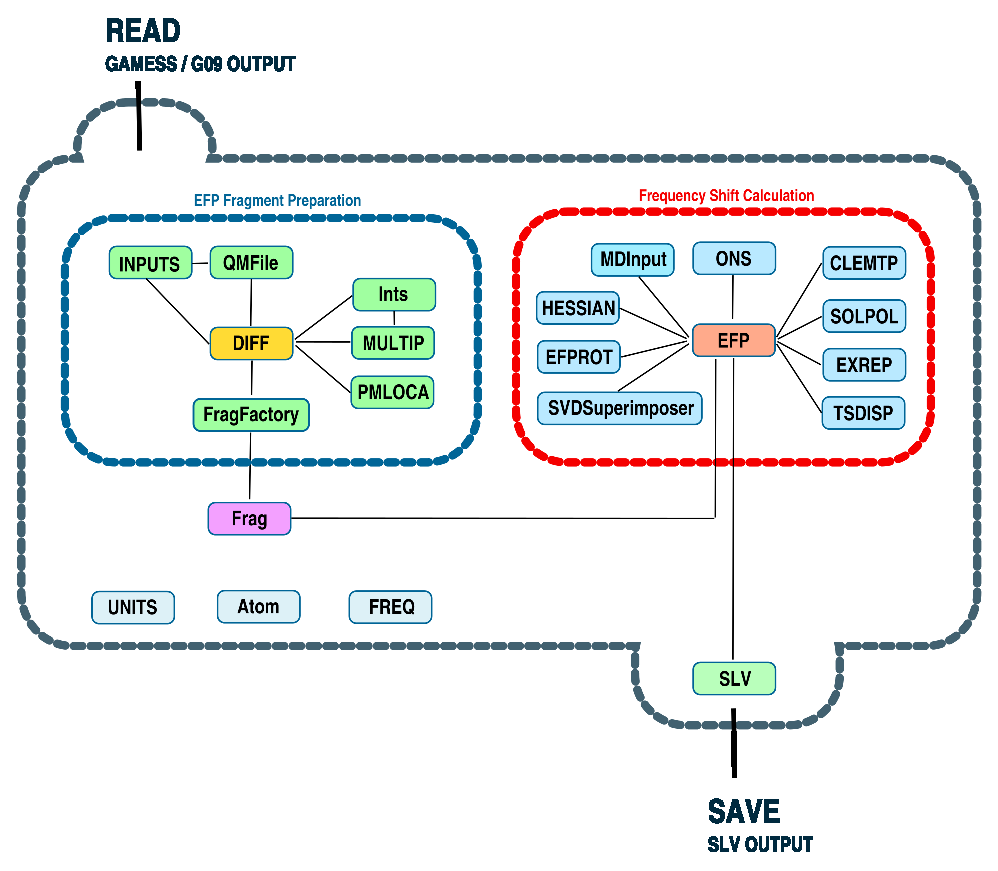
\includegraphics[width=0.90\linewidth]{slv-diagram.eps}
%}
\caption{
Structure of {\sc Solvshift}. The program imports the following 
{\sc Coulomb} modules: {\tt MULTIP}, {\tt QMFile}, {\tt Ints}, 
{\tt Freq}, {\tt Atoms} and {\tt UNITS}. Decisive classes
are highlighted by yellow (numerical differentiation), 
red (effective fragment potentials) and storage\hyp{}communication
classes are shown in violet.
\label{f:slv-structure}}
\end{figure}
%
It consists of two main modules: i) IBM fragment generators 
and ii) vibrational observable evaluators. The major driving classes
are {\tt DIFF} (which handles the numerical differentiations of
all the tensorial property), {\tt EFP} (with SolEFP equations)
and {\tt Frag} (describing an IBM object). Instances of {\tt Frag} are passed to
{\tt EFP} instance that sets and performs the calculations.

For the sake of efficiency, any type of one\hyp{}particle
density matrix (HF, MP2 or coupled cluster (CC))
as well as the coupled\hyp{}perturbed Hartree\hyp{}Fock calculations
are to be performed by external quantum chemistry packages.
The output files become the inputs for {\sc Solvshift}
which
processes them to produce output(s) on the screen
or output file(s).
On the other hand, one\hyp{}electron integral 
code\footnote{working on
the Gaussian Type Functions} is handled by {\sc Coulomb}
module \verb+Ints+. {\sc Coulomb} communicates with {\sc Solvshift}
also via distributed multipole analysis \verb+DMA+ objects which generalise
methods such as ESP charges, CAMM, DMA, LMTP, molecular multipole
moments or any other kind of multipole expansions. 
\verb+DMA+'s are therefore useful when working with
electrostatic SolX models such as SolCAMM etc.
For more specific information the Reader is referred 
to the SLV documentation.

\section{Usage}

Solvshift is very easy in use. It can be accessed 
from Python shell (like {\sc Coulomb} and any externally
available Python modules and packages\footnote{For example: NumPy, MDAnalysis, PyMol.}).
User can also communicate via command line using main {\tt slv} script.
SolEFP//CMD calculations are run by script {\tt slv{\textunderscore}md} which reads the
special input file.

\subsection{Steps of Setting Up EFP Environment for SLV Calculations}

The completely general way for defining the fragments within the target system
is through the input file. 
Instance of {\tt MDInput} class
will read the input file and will provide the appropriate fields to {\tt EFP} instance. 
The syntax of specifying one fragment
is shown in Figure~\ref{f:slv-inp-file-syntax}.
%
\begin{figure}[t!]
\centering
\setlength\fboxsep{0.4pt}
\setlength\fboxrule{0.5pt}
\begin{verbatim}
$Frag
  [name]     [(Sol)EFP parameter file]
  reorder    [reorder list]
  supl       [superimposition list]
  atoms      [atomic locations]             [number of EFP fragments]
  ...
$endFrag
\end{verbatim}
\caption{
The syntax of SolEFP input file for one fragment modelled by the
independent fragment molecule parameter object (IBM).
\label{f:slv-inp-file-syntax}}
\end{figure}
%
For example, for NMA--(H$_2$O)$_{918}$ system 
with water described by Tip4P model we could 
write the following input:
%
\begin{verbatim}
$Frag
    NMA     nma-d7
    reorder 1 3 5 2 7 10 11 12 4 6 8 9
    supl    0-4
    atoms   1-12                           1
$endFrag

$Frag
    water   water
    atoms   13-3684                        918
    supl    0-2
$endFrag
\end{verbatim}
%
First line refers to molecule name and file name with parameters. 
The names of built-in IBM's are listed in the first column
of Table~\ref{t:slv-ibm-buitin}.
However, it is also possible to generate a new IBM fragment file
by using fully automatised SLV routines.

We can reorder atoms in the next line
by keyword {\tt reorder [list]}. Also, we can provide 
superimposition list for that fragment. It can be
provided in this example either by {\tt 0 1 2 3 4} 
or {\tt 0-4} (both work the same). {\tt reorder} and {\tt supl} are
optional. The last entry or entries refer to atomic positions in CMD trajectory 
files and the number of
(Sol)EFP fragments. Note, that if frequency shift calculation is set, the first fragment
is assumed to be an IR probe molecule.\footnote{SLV can also perform
EFP2 interaction energy calculation and frequency shift calculation
can be switched off.} 
Note also that the turn of entries within one fragment is
arbitrary, except for the first line where fragment name and parameter file is provided. The more
detailed explanation and discussion about working with Tip4P water model and fragments of big
molecules is presented in Section~\ref{s:superimposition-practical}.

%If the order of atoms associated with a particular fragment differs between their parameter file
%and CMD file this has to be changed at the beginning of the calculation. 

%It is also extremely important to remember that the 
%object has to be properly placed in the space according to CMD frame. I.e., 
%rotation and translation
%has to be performed. 
%It is particularly important when dealing with fragments being parts of larger molecule. For instance --SO$_3$
%moiety can be described
%based on CH$_3$--SO$_3$ IBM.
%Here, we have to specify atoms of sulphonate groups and carbon atom in the
%backbone (just to properly place this fragment in space such that it is 
%superimposed with sulphonate group in target system). 

\subsection{Superimposition Problem\label{s:superimposition-practical}}

In order to provide the topology for SolEFP/EFP calculations it is necessary to specify where particular
SolEFP and EFP objects need to be superimposed within the structure from CMD trajectory. This brings
the need of explicit specifications of the atomic identities within EFP or SolEFP model fragment and their
assignment to the set of atoms in the target system. Since (Sol)EFP can be used not only to model
the same molecules but also certain fragments of larger molecules, the caution has to be kept because
the atomic orders will almost for sure be different when comparing (Sol)EFP model and the
corresponding fragment of the modelled system. Moreover, the atoms that correspond to the
(Sol)EFP model do not need to be in a continuous order -- there can be other atoms in between that
do not `belong' to the IBM model.

Therefore two constructs have been introduced to SLV to unambiguously define the relationships
between SolEFP/EFP and target topologies:
%
\begin{itemize}
\item Reordering lists
\item Superimposition lists
\end{itemize}
%
Those lists simply contain the atomic indices in some particular order or additional masks. In SLV, the
following convention is used: reordering lists refer to atomic indices in CMD (target) topology whereas
superimposition lists refer to (Sol)EFP atomic indices.
Here we discuss superimposition lists and atom rearrangement
in more detail. We shall do it on a few examples.

\subsubsection{Working with Tip4P Water Model}

Let us assume that in our CMD simulation file stores water molecules in the following order: 
O, H1, H2, X (for Tip4P model) where X is the additional non\hyp{}atomic
site near oxygen atom. On the other hand, our IBM water parameters
contain only 3 atoms in the order: O, H1, H2. Therefore we see from comparison that
%
\begin{verbatim}
   MD : O H1 H2 X
   EFP: O H1 H2
\end{verbatim}
%
so the corresponding superimposition list for water is [0,1,2] (we superimpose IBM onto CMD
fragment). In the input file we can specify this superimposition
list as {\tt supl 0-2} or {\tt supl 0 1 2}.

\subsubsection{Working with EFP Fragment Being a Part of Molecule}

It is more complicated and requires some caution. 
Let us first examine the tyrosine residue which is one of
building blocks of proteins (Figure~\ref{f:tyr-res-lists}).
%
\begin{figure}[t!]
\centering
\setlength\fboxsep{0.4pt}
\setlength\fboxrule{0.5pt}
%\fbox{
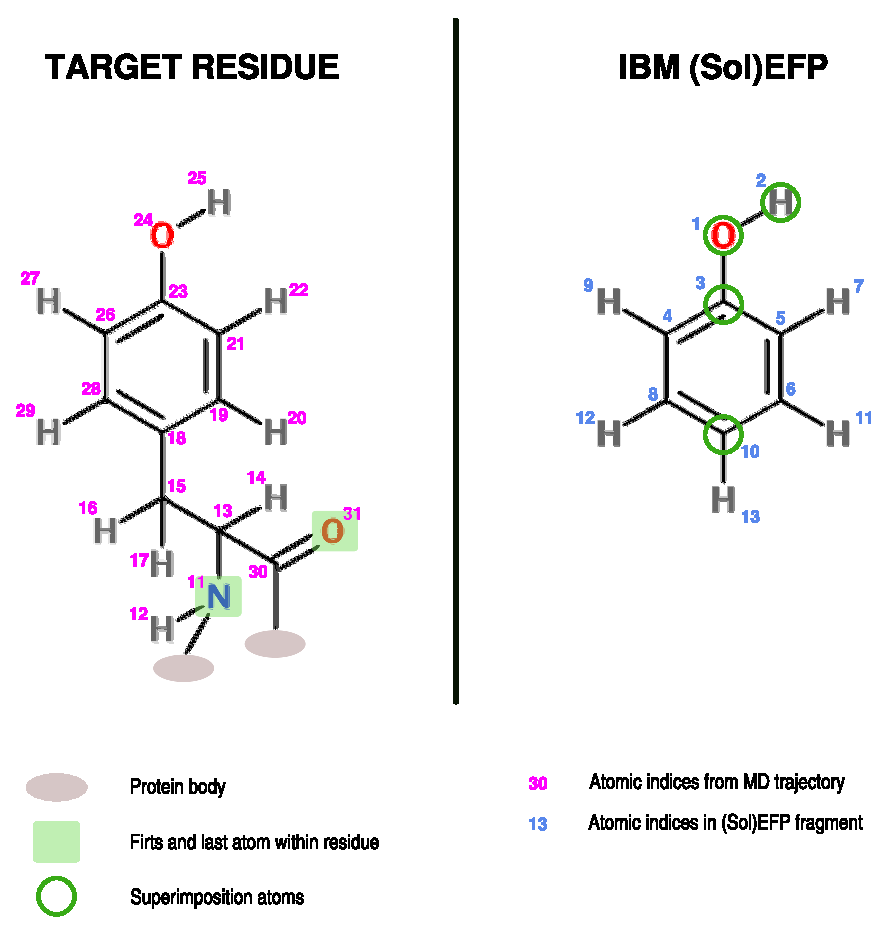
\includegraphics[width=0.92\linewidth]{m.reorder.eps}
%}
\caption{
Assignment of reordering and superimposition lists for Tyr residue
with phenol as a model EFP2 molecule. First atom is indicated by
number 1.
Tyr residue is assumed to be
a part of large peptide, hence the atomic numbers for that residue start
from 11 (for explanatory purposes).
\label{f:tyr-res-lists}}
\end{figure}
%
The first and last atoms in MD residue considered here are shown by green squares. In pink, the actual
atomic indices (starting from 1) are depicted. It is clear that the orders 
of atoms are completely different in IBM model and Tyr residue from CMD topology.

The following formula is used to determine the reordering list:
%
\begin{equation}   \label{e:reord-list}
{\rm reord}_i = 
\left\{\begin{matrix}
{\rm IDX}_{\rm CMD}^{(i)}
 - {\rm IDX}_{\rm First} + 1
                      & \text{If (Sol)EFP atom is in CMD topology}\\ 
0                     & \text{If (Sol)EFP atom is \emph{not} in CMD topology}
\end{matrix}\right.
\end{equation}
%
where ${\rm IDX}_{\rm First}$ is the index of the first atom 
within a given CMD topology residue.
The length of the {\tt reord} list is \emph{always} equal 
to the number of atoms in (Sol)EFP model. Thus
the reordering list will have 13 entries in this case.
To determine {\tt reord} and {\tt supl} we need to answer the following questions:
%
\begin{enumerate}
 \item Which atom in Tyr corresponds to first atom in IBM? Atom with index 24 -- but it is
14th atom within considered residue. So the first entry in {\tt reord} list is 14.
 \item Which atom in Tyr corresponds to seventh atom in EFP? Atom with index 22 -- but it is
12th atom within considered residue. So the 7th entry in {\tt reord} list is 12.
\item Which atom in Tyr corresponds to the last atom in EFP? Well, there is no corresponding
atom here. So this entry in reord list is 0.
\end{enumerate}
%
Thus, the final reord list for that example is 
%
\begin{verbatim}
   14, 15, 13, 16, 11, 9, 12, 18, 17, 8, 10, 19, 0
\end{verbatim}
%

The superimposition list has to be determined in such a way in order to prevent undefined EFP
orientations. In the example given above, we chose the superimposed atoms to be as indicated in green
open circles.
Why? Because only then we can be sure that the orientation of the OH group and the plane of the ring
is correct. The superimposition list is 
%
\begin{verbatim}
   1, 2, 3, 11
\end{verbatim}
%

As another example let us consider sulphonate group --SO$_3$
in organic sulphonates. It is attached to a carbon atom, but we want to consider only four atoms
and neglect the aliphatic chains. 
Let us assume that the order of the atoms in CMD file is: 
S, O1, O2, O3. However, our EFP fragment is based on methyl sulphonate anion CH$_3$--SO$_3^-$
for which the turn of atoms appears to be different: S, O1, O3, O2, C, H1, H2, H3. Note, that in our
example, EFP oxygen atoms have different absolute configuration than in CMD trajectory!\footnote{we have to treat
each atom as if it was different because of superimposition mathematics does not know atomic symbol,
just coordinate vectors!} So, even if we have the arrangement:
%
\begin{verbatim}
   MD : S O1 O2 O3
   EFP: S O1 O3 O2 C H1 H2 H3
\end{verbatim}
%
the corresponding reordering list is not [1,2,3,4]. In SLV, it is assumed
that the subset of atoms that is shared between CMD and EFP has the same order which also refers to the
absolute configuration! To adjust the not matching oxygens here we have to \emph{rearrange}
them as well. The correct list is
%
\begin{verbatim}
   1, 2, 4, 3
\end{verbatim}
%


\section{Summary and Outline of Future Development}

In this Chapter, we described briefly the {\sc Solvshift} package
which is believed to serve well for every member of Scientific Community
in the world who is interested in detailed understanding of the
vibrational solvatochromism phenomenon and explaining
the multidimensional vibrational spectra. It has parallel 
implementation which enables one to compute frequency shifts
for many frames at a time. It can also predict the changes in the
transition dipole moment within WCA limit. However, there is still a lot room for improvement.

It may be quite tedious to write the large input files manually especially when one has to analyse many
structures with different atomic indexing (for example when some fragments from CMD trajectory were
cut and saved in PDB file; topologies are still the same but the absolute atomic indices may be different.
Therefore, one can use the fact that the topology is constant and refer to the particular residues by their
name. In that case, the SLV input file with reordering and superimposing lists can be generated
automatically by the program. This feature is just initialised but need to be extended (we used
this only for certain forcefields implemented in {\sc Gromacs} for the purposes
of the analyses in Section~\ref{s:ral-solefp}).

The computation speed is very slow for evaluating the exchange\hyp{}repulsion and induction
contributions. The algorithm can be much improved to optimise the
evaluation of molecular integrals and inversions of sparse $\bf D$ matrices.
In the latter case, it is possible to design block algorithm which
will detect zero blocks in $\bf D$ matrices and subsequently speed up their
diagonalisations. It would also enable using larger $R_{\rm Max}$ cut\hyp{}offs.

The severe problem related to the differentiation of quantities that are
derived from the molecular orbital localisation is the molecular symmetry.
At present, we have designed the approximate algorithm of detecting the
molecular orbitals corresponding to various finite\hyp{}difference displaced
molecular structures. This algorithm is probably not working well in case of
symmetric orbitals present in, for example, MeCN molecule. This aspect needs 
to be carefully and, if necessary, definitely resolved.

Finally, it is desirable to use SolEFP\hyp{}based models for fragments
that are quite flexible in conformation. The structural rigidity of EFP
subunits can be partially overcome by generating a library of BSM's,
each having different conformation. The program could then automatically superimpose
all existing structural variations and choose one which is structurally the closest
to the target fragment.



\printbibliography[heading=subbibintoc,title={References}]
\end{refsection}

% ==================== APPENDICES ================================

\begin{appendices}
\addtocontents{toc}{\protect\setcounter{tocdepth}{0}}

\chapter{Tensor Notation\label{a:tensor-notation}}

Throughout the course of this Thesis, we have extensively used Cartesian tensors
of various ranks and the mathematical notation might be somewhat confusing
or unclear without explanation. Therefore, here we set the notational conventions
for dealing with tensor expressions and provide examples.

\section{Vectors}

We have used a usual dot product `$\cdot$' symbol to denote the following
operation
%
\begin{equation}
 {\bf a} \cdot {\bf b} \equiv \sum_\alpha a_\alpha b_\alpha
\end{equation}
%
whereas the outer product is denoted as `$\otimes$' symbol as
%
\begin{equation}
 {\bf a} \otimes {\bf b} = {\bf A} 
 \qquad\text{ such that } 
 \qquad A_{\alpha\beta}  \equiv a_\alpha b_\beta
\end{equation}
%
Note that ${\bf a} \otimes {\bf b} = \left( {\bf b} \otimes {\bf a} \right)^T \ne 
{\bf a} \otimes {\bf b}$ where the symbol `$T$' denotes the transposition 
of a matrix, $\left[ {\bf A}^T\right]_{\alpha\beta}=A_{\beta\alpha}$.

\section{Matrices}

The matrix\hyp{}matrix multiplication is defined as usual as
%
\begin{equation}
 {\bf A} {\bf B} = {\bf C} 
 \qquad\text{ such that } 
 \qquad C_{\alpha\beta}  \equiv \sum_\gamma A_{\alpha\gamma} B_{\gamma\beta} 
\end{equation}
%
We do not put the `$\cdot$' sign between ${\bf A}$ and ${\bf B}$ matrices 
in this case which means that the summation
goes over columns of ${\bf A}$ and rows of ${\bf B}$.

\subsection{Non-Symmetric Matrices}

Let us denote ${\bf A}$ to be a non-symmetric square matrix, i.e., 
$A_{\alpha\beta}\ne A_{\beta\alpha}$. To denote the matrix contractions
we use notation by explicitly using the symbol `$T$' if necessary.
Thus,
%
\begin{subequations}
\begin{align}
 {\bf A} \cdot {\bf b} &= {\bf c}
 \qquad\text{ such that } 
 \qquad c_{\alpha}  \equiv \sum_\gamma A_{\alpha\gamma} b_{\gamma} 
%
\\
{\bf b}^T \cdot {\bf A}   &= {\bf d}
 \qquad\text{ such that } 
 \qquad d_{\alpha}  \equiv \sum_\gamma b_{\gamma} A_{\gamma\alpha}
%
\\
{\bf b}^T \cdot {\bf A} \cdot {\bf c}  &= s
 \qquad\text{ such that } 
 \qquad s \equiv \sum_{\alpha\beta} b_{\alpha} A_{\alpha\beta} c_{\beta}
\end{align}
\end{subequations}
%
Note that ${\bf d} \ne {\bf c}$ and that 
${\bf b}^T \cdot {\bf A} \cdot {\bf c} \ne {\bf c}^T \cdot {\bf A} \cdot {\bf b}$.

\subsection{Symmetric Matrices}

In this Work, almost all of the matrices are symmetric, i.e., 
$A_{\alpha\beta}= A_{\beta\alpha}$. The only exceptions
are the ${\bf D}$ matrix from Eq.~\eqref{e:D-matrix} 
and its derivatives, of which the $3\times 3$ diagonal blocks
are in general non-symmetric (LMO\hyp{}distributed polarizabilities ${\BM \alpha}_a$
are non\hyp{}symmetric). 

The matrix\hyp{}vector\hyp{}to\hyp{}vector contractions are denoted as
%
\begin{equation}
 {\bf A} \cdot {\bf a} = {\bf a} \cdot {\bf A} = {\bf b} 
 \qquad\text{ such that } 
 \qquad b_\alpha \equiv \sum_{\beta} A_{\alpha\beta} b_{\beta} = \sum_{\alpha} b_{\alpha} A_{\alpha\beta} 
\end{equation}
%
The matrix\hyp{}matrix\hyp{}to\hyp{}scalar 
contractions are denoted
by using the ``symmetric double contraction''
symbol, `$:$' as
%
\begin{equation}
 {\bf A} : {\bf B} = s \qquad\text{ such that } 
                                   \qquad s \equiv \sum_{\alpha\beta} A_{\alpha\beta} B_{\alpha\beta}
\end{equation}
%
provided that at least one of the matrices ${\bf A}$ and ${\bf B}$ is symmetric.
We also often make use of the matrix\hyp{}vector\hyp{}vector\hyp{}to\hyp{}scalar contractions,
%
\begin{equation}
 {\bf A} : {\bf b} \otimes {\bf c} = {\bf A} : {\bf c} \otimes {\bf b} = s
 \qquad\text{ such that } 
 \qquad s \equiv \sum_{\alpha\beta} A_{\alpha\beta} b_{\alpha} c_{\beta}
\end{equation}
%

\section{Tensors of Rank 3 and Higher}

In this Thesis, only symmetric \nth{3} and \nth{4}\hyp{}rank Cartesian tensors,
i.e., each permutation of indices produces identical tensor, 
$T_{\cdots i\cdots j\cdots} = T_{\cdots j\cdots i\cdots}$.
Therefore, to perform tensor contractions, 
we use the ``symmetric $n$-tuple contraction operator''
acting symmetrically
with respect to the $K$th-rank tensors ${\bf T}^{(K)}$.
The outer product operator acts in a usual way, i.e.,
%
\begin{equation}
 {\bf T}^{(K_1)} \otimes {\bf T}^{(K_2)}  = {\bf T}^{(K_1+K_2)}
 \qquad\text{ such that } 
 \qquad T_{\underbrace{ij\cdots}_{K_1}\underbrace{kl\cdots}_{K_2}} \equiv 
 T_{\underbrace{ij\cdots}_{K_1}} T_{\underbrace{kl\cdots}_{K_2}} 
\end{equation}
%
For instance, the following operations are possible:
%
\begin{enumerate}
 \item tensor\hyp{}tensor\hyp{}to\hyp{}scalar contraction:
   %
   \begin{equation}
     {\bf T}^{(3)} \vdots {\bf S}^{(3)}  = s
     \qquad\text{ such that } 
     s \equiv 
     \sum_{\alpha\beta\gamma} T_{\alpha\beta\gamma} S_{\alpha\beta\gamma} 
   \end{equation}
   %
 \item tensor\hyp{}matrix\hyp{}to\hyp{}vector contraction:
   %
   \begin{equation}
     {\bf T}^{(3)} : {\bf A}^{(2)}  = {\bf a}^{(1)}
     \qquad\text{ such that } 
     a_\alpha \equiv 
     \sum_{\beta\gamma} T_{\alpha\beta\gamma} A_{\beta\gamma} 
   \end{equation}
   %
 \item tensor\hyp{}vector\hyp{}to\hyp{}matrix contraction:
   %
   \begin{equation}
     {\bf T}^{(3)} \cdot {\bf a}^{(1)}  = {\bf A}^{(2)}
     \qquad\text{ such that } 
     A_{\alpha\beta} \equiv 
     \sum_{\gamma} T_{\alpha\beta\gamma} a_{\gamma} 
   \end{equation}
   %
 \item tensor\hyp{}tensor\hyp{}to\hyp{}scalar contraction with outer product:
   %
   \begin{equation}
     {\bf T}^{(3)} \vdots {\bf a}^{(1)} \otimes {\bf A}^{(2)}  = s
     \qquad\text{ such that } 
     s \equiv 
     \sum_{\alpha\beta\gamma} T_{\alpha\beta\gamma} a_{\alpha} A_{\beta\gamma}
   \end{equation}
   %
 \item tensor\hyp{}tensor\hyp{}to\hyp{}vector contraction with outer product:
   %
   \begin{equation}
     {\bf T}^{(3)} : {\bf a}^{(1)} \otimes {\bf b}^{(1)}  = {\bf c}^{(1)}
     \qquad\text{ such that } 
     c_{\alpha} \equiv 
     \sum_{\beta\gamma} T_{\alpha\beta\gamma} a_{\beta} b_{\gamma}
   \end{equation}
   %
\end{enumerate}
%
The above examples are true when tensor ${\bf T}$ is symmetric, regardless
of the properties of other tensors. In the
above equations, we intentionally emphasised the rank of matrix (2)
and vector (1) to generalise our previous discussion.
We can notice that the number of dots in the $n$-tuple contraction operator
signals the number of summations that have to be performed. 

Similarly, we can have various expressions involving higher than \nth{3}\hyp{}rank
tensors. For example
   %
   \begin{equation}
     {\bf T}^{(4)} \vdots {\bf A}^{(2)} \otimes {\bf b}^{(1)}  = {\bf c}^{(1)}
     \qquad\text{ such that } 
     c_{\alpha} \equiv 
     \sum_{\beta\gamma\delta} T_{\alpha\beta\gamma\delta} A_{\beta\gamma} a_{\delta}
   \end{equation}
   %



\chapter{Molecular Vibrations\label{a:vibrational-analysis}}

To understand the theory of the vibrational solvatochromism 
discussed in detail in Section~\ref{s:theory}, it is customary
to be familiar with the theory behind the vibrational analysis
of a molecule build of $N$ atoms. First, we briefly discuss
the harmonic oscillator which is the basis of the consideration
when deriving the Buckingham's model of the vibrational solvatochromism.
Second, we describe the vibrational analysis of a polyatomic molecule
that is extensively used for calculations of \emph{ab initio} vibrational
harmonic frequencies in Chapters 5, 6 and 7. We do not discuss
the anharmonicity effects on the vibrational properties of molecules.
%which can be found elsewhere. %\citep{Barone.JCP.2005}

%\section{Matrix elements of $x^n$ operator in harmonic oscillator basis\label{a:matrix-elements}}
\section{The Harmonic Oscillator\label{a:harmonic-oscillator}}

The Hamiltonian of harmonic oscillator is given by
%
\begin{equation}\label{e:h_harm-appendix}
\mathscr{H}_{\rm Harm} = 
\frac{\hat{p}^2}{2M} + \frac{1}{2} M \omega^2 \hat{x}
\end{equation}
%
where $M$ is the reduced mass and $\hat{x}$ and $\hat{p}$ are the operators
of position and momentum, respectively. Solving the time\hyp{}independent 
Schr{\"o}dinger equation we find that 
%
\begin{equation}\label{e:h_harm-appendix-schreq}
\mathscr{H}_{\rm Harm} \vert n \rangle = 
E_n \vert n \rangle 
\end{equation}
%
where the energies $E_n=\hbar \omega \left( n+\frac{1}{2} \right)$ 
and eigenstates $\vert n \rangle$ can be found
in textbooks for quantum mechanics.

\subsection{Some Important Matrix Elements\label{a:matrix-elements}}

The following material is necessary for derivations of the Buckingham theory
of the vibrational frequency shifts that is presented in Sec.~\ref{s:buckingham-theory}. 

The matrix elements of the $x$ operator in the harmonic oscillator eigenstate basis set
can be found to be
%
\begin{equation}
\label{ea:mxn}
\langle n \vert \hat{x} \vert m \rangle = 
\sqrt{
\frac{\hbar}{2M\omega}
}
\left\{ 
   \sqrt{m+1} \delta_{n,m+1} + \sqrt{m} \delta_{n,m-1}
\right\}
\end{equation}
%
\noindent where $M$ is the reduced mass of the normal coordinate and $\omega$ is its 
angular frequency.

The evaluation of the matrix element of $\hat{x}^2=\hat{x}\hat{x}=\hat{x}\hat{1}\hat{x}$ 
operator is straightforward
by using the resolution of identity operator $\hat{1}$ and applying Eq.~\eqref{ea:mxn}
%
\begin{equation}
\langle n \vert \hat{x}^2 \vert m \rangle = 
\sum_{k=0}^{\infty} \langle n \vert \hat{x} \vert k \rangle \langle k \vert \hat{x} \vert m \rangle
\end{equation}
%
The final result is given by
%
\begin{equation} \label{ea:mxxn}
\langle n \vert \hat{x}^2 \vert m \rangle = 
\frac{\hbar}{2M\omega}
\Big\{ 
   (2m+1) \delta_{n,m} + \sqrt{(m+1)(m+2)} \delta_{n,m+2} + %\\
                         \sqrt{m(m-1)} \delta_{n,m-2}
\Big\}
\end{equation}
%
Following the same strategy one can easily find the expression for 
the matrix element of the $\hat{x}^3$ operator:
%
\begin{multline}
\label{ea:mxxxn}
\langle n \vert \hat{x}^3 \vert m \rangle = 
\left(
\frac{\hbar}{2M\omega}
\right)^{3/2}
\Big\{ 
   \sqrt{(m+1)(m+2)(m+3)} \delta_{n,m+3} + \\
   3(m+1)\sqrt{m+1} \delta_{n,m+1}
      +3m\sqrt{m}   \delta_{n,m-1} + \sqrt{m(m-1)(m-2)} \delta_{n,m-3}
\Big\}
\end{multline}
%
Note that diagonal matrix elements survive only for even operator $\hat{x}^2$
and vanish for all odd operators (it is true in general for all $\hat{x}^n$
operators). Thus, when expansions up to the third order in $\hat{x}$ are 
used, the only surviving contribution is
%
\begin{equation}
\label{ea:mxm}
\langle n \vert \hat{x}^2 \vert n \rangle = 
\frac{\hbar}{2M\omega}(2n+1)
\end{equation}
%
and, of course, $\langle n \vert n \rangle=1$ term.

\section{Vibrational Analysis of Polyatomic Molecule\label{asec:vibranal}}

The Hamiltonian of the vibrating molecule in equilibrium geometry under Born\hyp{}Oppenheimer approximation
can be expressed as the sum of Hamiltonians of independent harmonic oscillators:
\begin{equation}
\mathscr{H} = \sum_i \frac{1}{2M_i}\hat{{p}_i^2} + \mathscr{V}({\bf Q})
\end{equation}
In the above equation, $\mathscr{V}({\bf Q})$ denotes the vibrational potential energy function
expressed in normal coordinates, ${\bf Q}$. Under Harmonic approximation
\begin{equation}
\mathscr{V}({\bf Q}) = \frac{1}{2} \sum_i M_i \omega_i^2 Q_i^2
\end{equation}
and the reduced mass $M_i$ corresponds to the $i$th normal coordinate $Q_i$ with
harmonic frequency $\omega_i$.

To find a set of coordinates $Q$ that are orthogonal to each other (i.e., describe the normal 
modes of the molecule) one needs to consider a quadratic potential energy function
\begin{equation}
\mathscr{V}({\bf x}) = \frac{1}{2} \sum_i\sum_j \frac{\partial^2 E}{\partial x_i \partial x_j} x_i x_j
\end{equation}
and find such a similarity transformation that
\begin{equation}\label{eq:pot_harm}
\mathscr{V}({\bf Q}({\bf x})) = \frac{1}{2} \sum_i M_i \omega_i^2 Q_i^2({\bf x})
\end{equation}
or in matrix notation
\begin{equation}
\mathscr{V}({\bf x}) = \frac{1}{2} {\bf x}^{\dagger} {\bf H}^{\rm Cart} {\bf x}  
\quad \textrm{and   } \mathscr{V}({\bf Q}({\bf x})) = \frac{1}{2} {\bf Q}^{\dagger} {\bf H}^{\rm Q} {\bf Q} 
\end{equation}
Obviously ${\bf H}^{\rm Q}$ is diagonal whereas ${\bf H}^{\rm Cart}$ is not. 

Let us assume that
\begin{equation}
{\bf Q} = {\bf L}^{\dagger} {\bf x}
\end{equation}
with ${\bf L}$ unitary.
Therefore it is clear that
\begin{equation}
\mathscr{V}({\bf x}) = \frac{1}{2} {\bf x}^{\dagger} {\bf L} {\bf H}^{\rm Q} {\bf L}^{\dagger} {\bf x}
\end{equation}
or
\begin{equation}
{\bf H}^{\rm Q} = {\bf L}^{\dagger} {\bf H}^{\rm Cart} {\bf L}
\end{equation}
Therefore, diagonalising ${\bf H}^{\rm Cart}$ one can find the orthogonal 
set ${\bf Q}$. We note that the dimensions of ${\bf x}$ and ${\bf Q}$ are the unit distances.

\section{Mass-Weighted Coordinates\label{a:mw-coord}}

It is much better to express the normal coordinates in terms of the mass\hyp{}weighted coordinates.
To see this, let us assume that we want to get the frequencies from Eq.\eqref{eq:pot_harm} by diagonalising
the matrix ${\bf H}^{\rm Cart}$. Of course, we immediately obtain ${\bf L}$ and the force constants
in the normal modes expressed as Cartesian displacements (${\bf Q}$). But note that these force constants 
contain \emph{unknown} reduced masses.
Therefore the determination of vibrational harmonic frequencies is not yet possible. 

However, one could 
associate the reduced mass with the definition of the normal coordinate.
Let us try with changing to the Cartesian mass\hyp{}weighted coordinates defined by
\begin{equation}
\tilde{\bf x} = {\BM \Pi}{\bf x} 
\end{equation}
with
\begin{equation}
\Pi_{ij} = \delta_{ij} \sqrt{M_i}
\end{equation}
and rewrite the equations from Sec.\ref{asec:vibranal}.

By inserting ${\bf x}={\BM \Pi}^{-1}\tilde{\bf x}$ we get
\begin{equation}
\mathscr{V}(\tilde{\bf x}) = \frac{1}{2} \tilde{\bf x}^{\dagger} {\bf H}^{\rm MWC}  \tilde{\bf x}
\end{equation}
This corresponds to 
\begin{equation}
\mathscr{V}(\tilde{\bf Q}) = \frac{1}{2} \tilde{\bf Q}^{\dagger} {\bf H}^{\rm MWC,Q}  \tilde{\bf Q}
\end{equation}
expressed in \emph{mass-weighted} normal coordinates defined by
\begin{equation}
\tilde{Q}_i = \sqrt{M_i} Q_i
\end{equation}
and with 
\begin{equation}
H_{ij}^{\rm MWC,Q} = \delta_{ij} \omega_j^2
\end{equation}
Therefore, diagonalising mass-weighted Hessian in Cartesian coordinates (${\bf H}^{\rm MWC}$)
we can easily obtain the frequencies since they are equal to $\omega_j=\sqrt{H_{jj}^{\rm MWC,Q}}$.
Because we also have
\begin{equation}
{\bf H}^{\rm MWC,Q} = \tilde{\bf L}^{\dagger} {\bf H}^{\rm MWC} \tilde{\bf L}
\end{equation}
we can immediately find that
\begin{equation}
\tilde{\bf x} = \tilde{\bf L} \tilde{\bf Q}
\end{equation}
or in Cartesian not-weighted coordinates
\begin{equation}
{\bf x} = {\BM \Pi}^{-1} \tilde{\bf L} \tilde{\bf Q} = {\bf l} \tilde{\bf Q}
\end{equation}
where we introduced the matrix ${\bf l}={\BM \Pi}^{-1} \tilde{\bf L}$.

%--------------------------------------------------------------------------------------------------


\begin{refsection}
\chapter{Distributed Multipole Analysis\label{c:dma}}

In this Thesis we make use of the distributed multipole 
moments determined by using various methods in order to obtain
the appropriate vibrational solvatochromic models. In this Chapter,
we describe the mathematical formulation and characteristics of various methods
in more detail.
Under the distributed multipole approximation, the Coulombic
interaction energy operator can be expressed as a following series \citep{Stone.TheTheoryOfIntermolecularForces.1996}
%
\begin{equation} \label{e:a1100}
 \mathscr{U}^{\rm Coul} \cong \sum_{x\in A}\sum_{y\in B}  T^{xy}\hat{q}^{(x)}\hat{q}^{(y)} + 
\sum_\alpha T^{xy}_\alpha \left( \hat{q}^{(x)} \hat{\mu}^{(y)}_\alpha - \hat{\mu}^{(x)}_\alpha \hat{q}^{(y)}\right)
 - \sum_{\alpha\beta} T^{xy}_{\alpha\beta} \hat{\mu}^{(x)}_\alpha \hat{\mu}^{(y)}_\beta + \ldots
\end{equation}
%
where $x$ and $y$ denote the distributed sites on the solute and solvent
molecules, respectively. There exists a number of ways of obtaining
the distributed multipoles. 

\section{Traceless and Primitive Multipoles}

To compute interaction energy from Eq.~\eqref{e:a1100} one needs 
to use the ``traceless'' quadrupole and octupole moments. However, 
most of the operations performed on the distributed multipoles
are easier to handle when they are defined in ``primitive'' form.
This includes changing the origins of multipole moments.

Multipole $k$-rank tensor operators in ``primitive'' 
Cartesian form are defined as follows
%
\begin{equation} \label{e:m-operator}
\mathscr{M}^{(k)}({\bf r}_0) = \sum_i \hat{e}_i \underbrace{({\mathbf r}_i - {\bf r}_0) 
                      \otimes \cdots \otimes ({\mathbf r}_i - {\bf r}_0)}_{k}  \;.
\end{equation}
%
where $\hat{e}_i$ is the charge operator
and ${\bf r}_0$ is the origin of the multipole. 
For instance, dipole, quadrupole and octupole tensor 
operator elements are
%
\begin{eqnarray}\label{e:quadord}
\hat{\mu}_a         &=& \sum_i \hat{e}_i a_i \\
\hat{\Theta}_{ab}   &=& \sum_i \hat{e}_i a_i b_i \\
\hat{\Omega}_{abc}  &=& \sum_i \hat{e}_i a_i b_i c_i \quad  \textrm{where} \quad a,b,c=x-x_0,y-y_0 \; \textrm{or} \; z-z_0 \;.
\end{eqnarray}
%
%We shall drop now the `$\text{ }{\hat{}}\text{ }$' symbol and replace the operators
%with their expectation values.
Following Buckingham \citep{Buckingham.QRevChemSoc.1959}, the \emph{traceless} 
quadrupole 
moment operator is defined as follows
%
\begin{equation}\label{e:quadtraceless}
\hat{\Theta}_{ab}' = \frac{1}{2}\sum_i \hat{e}_i \big( 3a_ib_i-r_i^2\delta_{ab}\big)
\end{equation}
%
In the case of octupole moment the definition is a bit more 
complex:
\begin{equation}
\hat{\Omega}_{abc}' = \frac{1}{2}\sum_i \hat{e}_i   \big( 5a_ib_ic_i-r_i^2(a_i\delta_{bc}+
                                                                     b_i\delta_{ac}+
                                                                     c_i\delta_{ab})\big) 
\end{equation}
In the above equations $r_i^2$ equals to
%
%\begin{equation}\label{e:r2}
%$r_i^2 = \sum_{a=\{x,y,z\}} {a_i}^2   $.
$r_i^2 = \sum_a {a_i}^2   $.
%\end{equation}
%
It is very easy to switch from `primitive' tensor form to 
traceless one but the reversed transformation is not possible. 
The transition to traceless
quadrupole moment from ordinary Cartesian quadrupole moment 
can be done like in the example below. Rewriting 
Eq.~\ref{e:quadtraceless} and substituting the definition from 
\ref{e:quadord} one quickly obtains
%
\begin{equation}
\hat{\Theta}_{ab}' = \frac{3}{2}\sum_i \hat{e}_ia_ib_i - \frac{1}{2}\sum_i\sum_{\alpha}\hat{e}_i\alpha_i^2\delta_{ab} 
%= \frac{3}{2}\Theta_{ab} -\delta_{ab}\sum_{\alpha}\sum_ie_i\alpha_i^2 
= \frac{3}{2}\hat{\Theta}_{ab} - \frac{1}{2}\delta_{ab}\;\mathrm{Tr}\;\hat{\BM \Theta}  
\end{equation}
%
Similar calculations for traceless octupole moment give the
following expression
%
\begin{multline}
\hat{\Omega}_{abc}' = \frac{5}{2}\sum_i \hat{e}_ia_ib_ic_i - \frac{1}{2}\sum_i\sum_{\alpha}\hat{e}_i\alpha_i^2 \big(
                                        a_i\delta_{bc} + b_i\delta_{ac} + c_i\delta_{ab}  \big) \\ 
= \frac{5}{2}\hat{\Omega}_{abc} - \frac{1}{2} \big( \hat{\Omega}_{\alpha\alpha a}\delta_{bc} +
                                                \hat{\Omega}_{\alpha\alpha b}\delta_{ac} + 
                                                \hat{\Omega}_{\alpha\alpha c}\delta_{ab}  \big) 
\end{multline}
%
where $\hat{\Omega}_{\alpha\alpha c}$ denotes the trace of $\hat{\BM\Omega}$ 
tensor with respect to the first two axes written in Einstein
summation notation for simplicity. 

\section{DMA Method}

In the distributed multipole analysis 
(DMA) of Stone \citep{Stone.JCTC.2005}, the particular multipoles
are computed by integrating the matrix elements of multipole
operators over localised amount of volume enclosing the distributed
site of interest. Mainly,
%
\begin{equation}
{\bf M}^{(k)}_x  = \int_{V\ni x} {\rm d}\;{\bf r}
   \langle \Psi  \lvert \mathscr{M}^{(k)} ({\bf r}_x) \rvert  \Psi \rangle
\end{equation}
%
where $x$ refers to the distributed site placed at ${\bf r}_x$
and $V$ is the volume of space around it which is
determined by an appropriate algorithm. 
Multipole moments of this kind are characterised by good convergence
properties of the resulting interaction energies
if volumes $V$ are chosen correctly. 
However, differentiation of DMA with respect to nuclear coordinate
is difficult to handle in practice because the integration domains need to be the same
during numerical computation of the derivatives. Therefore, the DMA
procedures available in many quantum chemistry programs 
need to be reimplemented to adapt for numerical differentiation with respect
to normal modes.

\section{CAMM Method}

More convenient in use in the vibrational solvatochromic calculations
is the cumulative atomic multipole
moments method (CAMM) developed by Sokalski and Poirier. \citep{Sokalski.Poirier.CPL.1983}
The multipoles are the generalisation of the Mulliken atomic charges
and they are given by exact relations:
%
\begin{subequations}
\begin{align}
q_x              &=Z_x -\sum_{r\in x} \sum_s  P_{rs} \langle r \rvert s \rangle \\
\bm{\upmu}_x     &= \sum_{r\in x} \sum_s  P_{rs} 
\left[
        \langle r \rvert s \rangle {\bf r}_x - \langle r \lvert {\bf r} \rvert s \rangle
\right]   \\
\bm{\Theta}_{x}  &= \sum_{r\in x} \sum_s P_{rs}
\left[
   - {\bf r}_x \otimes {\bf r}_x \langle r \rvert s \rangle +
    {\bf r}_x \otimes  \langle r \lvert {\bf r} \rvert s \rangle + 
                       \langle r \lvert {\bf r} \rvert s \rangle \otimes {\bf r}_x -
    \langle r \lvert {\bf r} \otimes {\bf r} \rvert s \rangle
\right]   \\
%\begin{gathered}
\bm{\Omega}_{x}  &=
\sum_{r\in x} \sum_s P_{rs}
\Big[
          {\bf r}_x \otimes {\bf r}_x \otimes {\bf r}_x \langle r \rvert s \rangle -
          {\bf r}_x \otimes {\bf r}_x \otimes \langle r \lvert {\bf r} \rvert s \rangle -
          {\bf r}_x \otimes \langle r \lvert {\bf r} \rvert s \rangle \otimes {\bf r}_x \nonumber \\ 
 &\quad- \langle r \lvert {\bf r} \rvert s \rangle \otimes {\bf r}_x \otimes {\bf r}_x +
          {\bf r}_x \otimes \langle r \lvert {\bf r} \otimes {\bf r} \rvert s \rangle +
          \langle r \lvert {\bf r} \otimes {\bf r}_x \otimes {\bf r} \rvert s \rangle +
          \langle r \lvert {\bf r} \otimes {\bf r} \rvert s \rangle \otimes {\bf r}_x \nonumber \\ 
 &\quad- \langle r \lvert {\bf r} \otimes {\bf r} \otimes {\bf r} \rvert s \rangle
\Big] 
%\end{gathered}
\end{align}
\end{subequations}
%
where $r$ and $s$ denote the basis functions, $P_{rs}$ is the
one\hyp{}particle density matrix element and $x$ is the atomic centre
with atomic number $Z_x$.
All the one\hyp{}electron multipole integrals 
$\langle r \lvert f({\bf r},{\bf r}_x)\rvert s \rangle$ 
can be easily 
evaluated by a computer program using the above analytical formulae.
Therefore, there is no technical problem related to the differentiation of CAMM
with respect to the nuclear coordinate.\footnote{One needs to pay attention
upon keeping the origins of multipoles fixed during the numerical differentiation}
%see the discussion on that aspect in Sec.XXX} 
However, the convergence of CAMM
is somewhat worse than that of DMA since the integration of matrix elements 
is performed over the whole space. This means that the electronic density
is divided evenly over all atomic orbitals, even those which are located far
from the distribution centre. Nevertheless, CAMM still provides reasonable 
estimates of $U^{\rm Coul}$ and we have used them throughout this Thesis.

\section{LMTP Method}

Instead of using atoms as expansion centers, one can use also localised molecular orbitals
for that purpose. This is the localised orbital multipole (LMTP) expansion 
proposed by Etchebest \emph{et al}. \citep{Etchebest.Lavery.Pullman.TheorChimActa.1982}
The aim is to decompose molecular multipole moments into additive
distributed moments which are centred not only at atomic sites
(and even at mid\hyp{}bond distances) but also at lone\hyp{}pairs 
and extended $\pi$\hyp{}orbitals in a way similar to the Mulliken\hyp{}based
partitioning scheme.

The molecular primitive and origin\hyp{}dependent multipole moment $\bf M$
is given as:
%
\begin{equation}\label{M}
{\bf M} ({\bf r}_0) = \sum_x Z_x\left({\bf r}_x - {\bf r}_0 \right)  
                    + \tbraket{\Psi}{\mathscr{M}^{(k)}_{\rm el}({\bf r}_0) }{\Psi}
\end{equation}
%
%where $\mathscr{M}^{(k)}$ is $k$th rank multipole moment operator
%
%\begin{equation}\label{Mop}
%\mathscr{M}^{(k)} = -\sum_i^N \underbrace{{\bf r}_i \otimes \cdots \otimes {\bf r}_i }_{r \; {\rm times}} = \sum_i^N \hat{m}^{(r)}(N)
%\end{equation}
%
where $\mathscr{M}^{(k)}_{\rm el}({\bf r}_0)$ denotes the electronic
part of the operator in Eq.~\eqref{e:m-operator} and
$Z_x$ is the atomic number of $x$th atom.
%The summation extend over all atoms and all electrons $i$ in the system
%and $\otimes$ is tensor outer product operator.
It can be easily shown that
%
\begin{equation}\label{MSC}
{\bf M}({\bf r}_0) = \sum_x Z_x\left({\bf r}_x - {\bf r}_0 \right) 
                   + \sum_i^N \tbraket{\chi_i}{\mathscr{M}^{(k)}_{\rm el}({\bf r}_0)}{\chi_i}
\end{equation}
%
in which $\ket{\chi_i}$ denotes the occupied molecular spin\hyp{}orbital.
Now let us define a simple decomposition of electronic part of $\bf M$, i.e. ${\bf M}_e$:
%
\begin{equation}\label{MSCp}
{\bf M}_e({\bf r}_0) = \sum_G {\bf M}_{e,G}({\bf r}_0) 
                     = \sum_G \sum_{i \in G} \tbraket{\chi_i}{\mathscr{M}^{(k)}_{\rm el}({\bf r}_0)}{\chi_i}
\end{equation}
%
Now, if we want to start from canonical orbitals $\ket{\chi_i}_C$ and use atomic basis functions to create also
non\hyp{}atomic and non\hyp{}mid\hyp{}bond distributed moments one should rather use in Equation \eqref{MSCp} localised
molecular spin\hyp{}orbitals, $\ket{\chi_i}_L$:
%
\begin{equation}\label{a}
\ket{\chi_i}_L = \sum_j U_{ji} \ket{\chi_i}_C
\end{equation}
%
where $\bf U$ is unitary rotation matrix in space of canonical MOs which localises them
and can be obtained by, for instance, the Pipek\hyp{}Mezey method. \citep{Pipek.Mezey.JCP.1989}
Assuming we know
$U_{ji}$ elements and using LCAO expansion of canonical MO one immediately finds that
%
\begin{equation}\label{b}
{\bf M}_{e,G}({\bf r}_0) = \sum_{i \in G} \sum_{jm} \sum_{\lambda\sigma} U^*_{ji} U_{mi} C^*_{j\lambda} C_{m\sigma}
   \tbraket{\lambda}{\mathscr{M}^{(k)}_{\rm el}({\bf r}_0)}{\sigma}
\end{equation}
%
Here, $C_{j\lambda}$ are canonical expansion coefficients of MO in AO basis. Note that the
operator $\mathscr{M}^{(k)}_{\rm el}({\bf r}_0)$ is a one\hyp{}electron operator
and evaluation of its matrix elements in AO basis is very efficient. However, 
note also that ${\bf M}_{e,G}$ is still defined with respect to the \emph{molecular} origin at $({\bf r}_0)$
and it has to be \emph{recentered} to the origin suitable for a particular group $G$ (see the
next Section~\ref{s:multipole-recentering}).

When we evaluate all the moments for each LMO group $G$ we can accumulate them in each $G$th centre
changing the origins. There are always MOs which are centred mainly on atoms (atomic contributions
mostly from core AOs) but there will be many non-atomic centers which will contribute to bond, lone pair
as well as $\pi$\hyp{}orbital distributed moments, respectively. The centers can be grouped to reduce the number
of expansion centers. The part of $\bf M$ which comes from atomic
nuclei can be just added to electronic atomic moments.

\section{Changing the Origins of Multipole Moments\label{s:multipole-recentering}}

Here we describe the recentering of DMA/CAMM/LMTP origins which can be used
to compute total multipole moments from distributed moments (evaluation SolMMM from SolCAMM parameters)
or obtain the united atom (contracted) SolCAMM models (see Figure~\ref{f:contr}).

We derived the direct formulae that can be implemented in a vectorised manner. 
Thus, the multipole moments
defined with respect to new origin ${\bf r}_N$ and old origin ${\bf r}_N$ are related as follows
%
\begin{subequations}
\begin{align}
q({\bf r}_N)               &= q({\bf r}_O)  \\
{\BM \upmu}({\bf r}_N)       &= {\BM \upmu}({\bf r}_O) - q({\bf r}_O) {\bf D}_1 \\ 
{\BM \Theta}({\bf r}_N)    &= {\BM \Theta}({\bf r}_O) + q({\bf r}_O) {\bf D}_2 \nonumber \\  
 &- {\BM \upmu}({\bf r}_O) \otimes {\bf D}_1 - {\bf D}_1 \otimes {\BM \upmu}({\bf r}_O)  \\  
{\BM \Omega}({\bf r}_N)    &= {\BM \Omega}({\bf r}_O) - q({\bf r}_O) {\bf D}_3 \nonumber \\ 
 &+ {\BM \upmu}({\bf r}_O) \otimes {\bf D}_2 + {\bf D}_2 \otimes {\BM \upmu}({\bf r}_O) \nonumber \\ 
 &+ {\bf r}_N \otimes {\BM \upmu}({\bf r}_O) \otimes {\bf r}_N - {\bf r}_O \otimes {\BM \upmu}({\bf r}_O) \otimes {\bf r}_O \nonumber \\ 
 &- [{\bf r}_N \otimes {\BM \Theta}({\bf r}_O)]_{1,0,2} + [{\bf r}_O \otimes {\BM \Theta}({\bf r}_O)]_{1,0,2} 
\end{align}
\end{subequations}
%
where the auxiliary displacement tensors are
%
\begin{subequations}
\begin{align}
{\bf D}_1 &= {\bf r}_N - {\bf r}_O \\
{\bf D}_2 &= {\bf r}_N \otimes {\bf r}_N  - {\bf r}_O \otimes {\bf r}_O  \\
{\bf D}_3 &= {\bf r}_N \otimes {\bf r}_N \otimes {\bf r}_N  - {\bf r}_O \otimes {\bf r}_O \otimes {\bf r}_O
\end{align}
\end{subequations}
%
and transposed 1-2 outer product is defined to be
%
\begin{equation}
\left( [{\bf a} \otimes {\bf A} ]_{1,0,2} \right)_{ijk} = a_j A_{ik}
\end{equation}
%
for any vector ${\bf a}$ and second-rank tensor ${\bf A}$.

\printbibliography[heading=subbibintoc,title={References}]
\end{refsection}

% ---------------------------------------------------------------------------------------------------
\chapter{Correction Terms for Evaluation of $\Delta \omega^{\rm Coul}$\label{a:fk-terms}}

Here we list the explicit formulae for the evaluation of the first and second derivatives
of the solute\hyp{}solvent interaction potential that emerge due to the electrostatic potential
variation along the solute's normal coordinate. Subsequently, the series 
convergence properties are tested for model NMA-H$_2$O dimers. 
Refer to Eq.~\eqref{e:dw-solefp-coul-correction}
for the context.

\section{Asymptotic Analysis of the Correction Terms}

After inserting the series expansions from Eq.~\eqref{e:potential-gradients} 
and Eq.~\eqref{e:interaction-tensors} into Eqs.~\eqref{e:f-terms} and \eqref{e:k-terms}
one can easily see that each term containing interaction tensors of various ranks
will have different asymptotic behaviours which can be put in 
the following rule:
%
\begin{quote}
The term containing interaction tensor of rank $n$ 
has $r^{-(n+1)}$ asymptotic dependence.
\end{quote}
%
Following this rule,
it is easy to see that considering the dependence up to $r^{-4}$ among the new terms
there are two $r^{-2}$ terms, five $r^{-3}$ terms and eight
$r^{-4}$ terms, so fifteen terms in total. Comparing with 
solvatochromic multipole terms when one has two $r^{-1}$,
four $r^{-2}$, six $r^{-3}$ and eight $r^{-4}$ terms (20 in total)
the amount of the new terms is quite big though there are no $r^{-1}$ 
terms present. In Table~\ref{t:cterms} all the terms for $n=2,3,4$
are listed and grouped to simplify the expressions.

\begin{table}[ht]
%\resizebox{1.4\textwidth}{!}{\begin{minipage}{\textwidth}
\caption{List of the additional terms originating from the
electrostatic interaction that were not included in $\Delta\omega^{\rm SolDMA}$.
Here, the subscripts or superscripts $x$ and $y$ refer to the distributed multipole
sites of the solute and solvent molecules, respectively. To simplify notation,
we used the definitions: $G^{(i)}_{xy} \equiv {\bf L}_x^{(i)} \cdot {\bf r}_{xy}$,
$G_{x;xy}^{(i)} \equiv {\BM \mu}_x \cdot {\bf L}_x^{(i)}$, $G_{y;xy}^{(i)} \equiv {\BM \mu}_y \cdot {\bf L}_x^{(i)}$
and $G_{x;xy}^{(i,\partial)} \equiv \fderiv{{\BM \mu}_x}{Q_i} \cdot {\bf L}_x^{(i)}$.
It is assumed that the derivatives are computed at the solute's gas-phase geometry.
\label{t:cterms}}
%\begin{footnotesize}
\begin{tabular*}{1.0\textwidth}{@{\extracolsep{\fill} } l ll ll}
\hline\hline
$r^{-n}$        && $U_i^{(x,y)}$   && $U_{jj}^{(x,y)}$ \\%[10ex] 
\hline
$r^{-2}$        && $-q_xq_y r_{xy}^{-3} G^{(i)}_{xy}$  
                && $-2\fderiv{q_x}{Q_j}q_y r_{xy}^{-3} G^{(j)}_{xy}$ \\
\hline
\multirow{3}{*}{$r^{-3}$}  && $-3G^{(i)}_{xy} r_{xy}^{-5} \left( q_x {\BM \mu}_y  -q_y {\BM \mu}_x \right) \cdot {\bf r}_{xy}$  
                           && $-6G^{(j)}_{xy} r_{xy}^{-5} \left( \fderiv{q_x}{Q_j} {\BM \mu}_y  -q_y \fderiv{{\BM \mu}_x}{Q_j} \right) \cdot {\bf r}_{xy}$ \\
                           && $r_{xy}^{-3} \left( q_x {\BM \mu}_y  -q_y {\BM \mu}_x \right) \cdot {\bf L}_x^{(i)}$ 
                           && $2r_{xy}^{-3} \left( \fderiv{q_x}{Q_j} {\BM \mu}_y  
                                                -q_y \fderiv{{\BM \mu}_x}{Q_j} \right) \cdot {\bf L}_x^{(j)}$ \\
                           && 
                           && $q_xq_y\left( 3\left(G^{(j)}_{xy}\right)^2 r_{xy}^{-2} - 
                                  \left| {\bf L}_x^{(j)} \right|^2\right)r_{xy}^{-3}$\\
\hline
\multirow{8}{*}{$r^{-4}$}  && $2r_{xy}^{-5} \left( q_x{\BM \Theta}_y + q_y{\BM \Theta}_x \right) : {\bf L}_x^{(i)} \otimes {\bf r}_{xy}$  
                           && $4r_{xy}^{-5} \left( \fderiv{q_x}{Q_j}{\BM \Theta}_y 
                              + q_y\fderiv{{\BM \Theta}_x}{Q_j} \right) : {\bf L}_x^{(j)} \otimes {\bf r}_{xy}$ \\
                           && $-5G^{(i)}_{xy} r_{xy}^{-7} \left( q_x{\BM \Theta}_y 
                              + q_y{\BM \Theta}_x \right) : {\bf r}_{xy} \otimes {\bf r}_{xy}$ 
                           && $-10G^{(j)}_{xy} r_{xy}^{-7} \left( \fderiv{q_x}{Q_j}{\BM \Theta}_y 
                              + q_y\fderiv{{\BM \Theta}_x}{Q_j} \right) : {\bf r}_{xy} \otimes {\bf r}_{xy}$\\
                           && $-3\left(G^{(i)}_{xy} {\BM \mu}_x \cdot {\BM \mu}_y
                              + G_{y;xy}^{(i)} {\BM \mu}_x \cdot {\bf r}_{xy}
                                     \right)r_{xy}^{-5}$ 
                           && $-6\left(G^{(j)}_{xy} \fderiv{{\BM \mu}_x}{Q_j} \cdot {\BM \mu}_y
                              + G_{y;xy}^{(j)} \fderiv{{\BM \mu}_x}{Q_j} \cdot {\bf r}_{xy}
                                     \right)r_{xy}^{-5}$ \\
                           && $-3 G_{x;xy}^{(i)} r_{xy}^{-5} {\BM \mu}_y \cdot {\bf r}_{xy}$
                           && $-6 G_{x;xy}^{(j,\partial)}r_{xy}^{-5} {\BM \mu}_y \cdot {\bf r}_{xy}$ \\
                           && $15G^{(i)}_{xy} r_{xy}^{-7} {\BM \mu}_x \otimes {\BM \mu}_y : {\bf r}_{xy}^2 $ 
                           && $30G^{(j)}_{xy} r_{xy}^{-7} \fderiv{{\BM \mu}_x}{Q_j} \otimes {\BM \mu}_y : {\bf r}_{xy}^2 $\\
                           && 
                           && $15r_{xy}^{-7} \left(G^{(j)}_{xy}\right)^2 \left( q_x{\BM \mu}_y 
                              - q_y{\BM \mu}_x \right) \cdot {\bf r}_{xy} $ \\
                           &&  
                           && $-3q_x r_{xy}^{-5} \left( 2G^{(j)}_{xy} {\bf L}_x^{(j)} 
                              + \left(G^{(j)}_{xy}\right)^2 \right) \cdot {\BM \mu}_y $ \\
                           &&  
                           && $+3q_y r_{xy}^{-5} \left( 2G^{(j)}_{xy} {\bf L}_x^{(j)} 
                              + \left(G^{(j)}_{xy}\right)^2 \right) \cdot {\BM \mu}_x $ \\
\hline\hline
\end{tabular*}
%\end{footnotesize}
%\end{minipage} }
\end{table}


\section{Analysis of the Convergence Properties of Eq.~\eqref{e:dw-solefp-coul-correction}\label{a:convergence-of-the-correction-terms}}

We have analysed the various contributions to $\Delta\omega^{\rm Coul}(\partial\phi)$
for the three model systems A, B and C depicted in Fig.~\ref{f:nma-abcde}. It is found 
(Table~\ref{t:ctest}) that
it is safe to truncate the series expansion on $r^{-2}$ terms. The other higher order terms,
especially in the case of the electronic anharmonicity contribution 
(associated with $U_{jj}$), can cause unreasonably
large frequency shifts. 
We compare the approximate evaluation with SolEDS calculations as a benchmark frequency shifts.

\begin{table}[ht]
\caption{Convergence of the electrostatic correction terms to SolCAMM
method that were estimated for three model NMA-H$_2$O dimers (A, B, C)
shown in Figure~\ref{f:nma-abcde}. In this Table, `MEA' and `EA' denote the mechanical and electric
anharmonicity contributions, respectively, whereas `Total' is their sum.
Cumulative atomic multipole moments (CAMM) were evaluated 
at all atoms of NMA with subsequent contraction of CH$_3$ groups 
to get SolCAMM-6 model.
Calculations were performed at HF/6-311++G** level.
All values are given in cm$^{-1}$.
\label{t:ctest}}
\begin{tabular*}{1.0\textwidth}{@{\extracolsep{\fill} } l ll ll}
\hline\hline
\multicolumn{5}{c}{Amide I mode} \\
\hline
System               & Method    & MEA           & EA         & Total        \\
\hline
\multirow{5}{*}{A}   & SolCAMM   & -39.4 (+6.2)  & 5.3 (+0.9) & -34.1 (+7.1) \\
        & Corr$^{\rm r2}$        & -47.4 (-1.8)  & 4.9 (+0.5) & -42.5 (-1,3) \\
        & Corr$^{\rm r2+r3}$     & -53.2 (-7.6)  & 7.7 (+3.3) & -45.5 (-4.3) \\
        & Corr$^{\rm r2+r3+r4}$  & -55.3 (-9.7)  & 8.8 (+4.4) & -46.5 (-5.3) \\
                     & SolEDS    & -45.6         & 4.4        & -41.2        \\
\hline
\multirow{5}{*}{B}   & SolCAMM   & -15.2 (+1.7)  & 3.8 (+2.2) & -11.4 (+3.9) \\
        & Corr$^{\rm r2}$        & -17.7 (-0.8)  & 4.3 (+2.7) & -13.4 (+1.9) \\
        & Corr$^{\rm r2+r3}$     & -21.1 (-4.2)  & 4.0 (+2.4) & -17.1 (-1.8) \\
        & Corr$^{\rm r2+r3+r4}$  & -21.2 (-4.3)  & 3.7 (+2.1) & -17.5 (-2.2) \\
                     & SolEDS    & -16.9         & 1.6        & -15.3        \\
\hline
\multirow{5}{*}{C}   & SolCAMM   & -35.4 (+6.6)  & 8.9 (+3.3) & -26.5 (+9.9) \\
        & Corr$^{\rm r2}$        & -40.7 (+1.3)  & 8.8 (+3.2) & -31.9 (+4.5) \\
        & Corr$^{\rm r2+r3}$     & -41.6 (+0.4)  &11.9 (+6.3) & -29.7 (+6.7) \\
        & Corr$^{\rm r2+r3+r4}$  & -42.6 (-0.6)  &15.0 (+9.4) & -27.6 (+8.8) \\
                     & SolEDS    & -42.0         & 5.6        & -36.4        \\
\hline\hline
\multicolumn{5}{c}{Amide II mode} \\
\hline
System               & Method    & MEA           & EA         & Total        \\
\hline
\multirow{5}{*}{A}   & SolCAMM   & 14.0 (+2.9)   & -6.3 (-3.2)& 7.7 (-0.3)   \\
        & Corr$^{\rm r2}$        & 14.3 (+3.2)   & -6.4 (-3.3)& 7.9 (-0.1)   \\
        & Corr$^{\rm r2+r3}$     & 14.0 (+2.9)   & -7.2 (-4.3)& 6.8 (-1.2)   \\
        & Corr$^{\rm r2+r3+r4}$  & 15.0 (+3.9)   & -8.2 (-5.1)& 6.8 (-1.2)   \\
                     & SolEDS    & 11.1          & -3.1       & 8.0          \\
\hline
\multirow{5}{*}{B}   & SolCAMM   & 10.6 (-1.1)   & 13.2 (+8.4)& 23.8 (+7.3)  \\
        & Corr$^{\rm r2}$        & 13.4 (+1.7)   & 13.2 (+8.4)& 26.6 (+10.1) \\
        & Corr$^{\rm r2+r3}$     & 19.1 (+7.4)   & 22.0 (+17.2)&41.1 (+24.6) \\
        & Corr$^{\rm r2+r3+r4}$  & 21.6 (+9.9)   & 42.1 (+37.3)&63.7 (+47.2) \\
                     & SolEDS    & 11.7          & 4.8        & 16.5         \\
\hline
\multirow{5}{*}{C}   & SolCAMM   & 12.8 (+1.2)   & -4.9 (-2.9)& 7.9 (-1.7)   \\
        & Corr$^{\rm r2}$        & 14.4 (+2.8)   & -4.9 (-2.9)& 9.5 (-0.1)   \\
        & Corr$^{\rm r2+r3}$     & 14.6 (+3.0)   & -5.4 (-3.4)&11.0 (+1.4)   \\
        & Corr$^{\rm r2+r3+r4}$  & 14.7 (+3.1)   & -5.6 (-3.6)& 9.1 (-0.5)   \\
                     & SolEDS    & 11.6          & -2.0       & 9.6          \\
\hline\hline
\end{tabular*}
\end{table}
%--------------------------------------------------------------------------------------------------


% ---------------------------------------------------------------------------------------------------------------
\begin{refsection}
\chapter{Computational Details\label{a:computational-details}}

Here we provide the details of computation for Chapters 5, 6 and 7.

\section{Chapter 5}

$N$-methylacetamide (NMA) and its deuterated molecule
(NMA-$d$ with deuterium at its amide position) 
were chosen as model IR active solute molecules. 
Gas phase equilibrium
geometry optimisations and vibrational analyses of NMA
and NMA-$d$ were performed
to obtain harmonic vibrational frequencies, reduced
masses and eigenvectors.
We mark here that the harmonic frequencies were not scaled. 
For all structure optimisations the convergence
threshold of energy gradient was set to be 10$^{-6}$~a.u.
which is a very tight criterion.
Here, the Density Functional Theory (DFT) B3LYP \citep{Becke.JCP.1993,
Lee.Yang.Parr.PhysRevB.1988,Vosko.Wilk.Nusair.CJP.1980,
Stephens.Devlin.Chabalowski.Frisch.JPC.1994}
%
or Hartree Fock \citep{Roothaan.RevModPhys.1951} (HF) methods were used,
with Cartesian 6-311++G** 
basis set \citep{Krishnan.Binkley.Seeger.Pople.JCP.1980,
McLean.Chandler.JCP.1980}.\footnote{It is 
important \emph{not} to use spherical harmonic bases
because we have implemented only Cartesian basis sets 
in our code. Therefore, the results will not be consistent
with {\sc Solvshift} and {\sc Coulomb} if one used spherical basis sets!} 
Cubic anharmonic constants were obtained from the numerical
differentiation of the Hessian matrices retrieved from Gaussian
formatted checkpoint ({\tt fchk}) files.
It is to be emphasised here that the cubic anharmonic constants
that can be also calculated using Barone's implementation \citep{Barone.JCP.2005} 
of
the vibrational second\hyp{}order perturbation theory,
cannot be used for SolEFP and SolEDS calculations because of the mismatch of the eigenvector
phases.

In all the calculations, SCF convergence threshold
was set to 10$^{-10}$~a.u. for density matrix and dense grid with
199 radial shells per atom and 974 angular points for each
shell for numerical integration were 
applied. \citep{Lebedev.Skorokhodov.RussAcadSciDoklMAth.1992}
Geometry optimisations and vibrational analyses were carried out
by using {\sc Gaussian 09} program. \citep{Frisch.Gaussian.2009}

\subsection{Onsager Model}

Self\hyp{}Consistent Reaction Field (SCRF) calculations
using Onsager model \citep{Kirkwood.JCP.1934,Onsager.JACS.1936,
Wong.Frisch.Wiberg.JACS.1991,Wong.Wiberg.Frisch.JCP.1991,
Wong.Wiberg.Frisch.JACS.1992}
%
with the cavity radius of
$a$ = 3.72~\AA, were performed by using the {\sc Gaussian 09} program package. \citep{Frisch.Gaussian.2009}
The vibrational frequency shifts from that calculations can be directly
compared with our continuum vibrational solvatochromism model
based on Onsager theory. In the flexible model (including structural
distortions) the threshold for converging the solvation energy
was set to be 10$^{-14}$ a.u. and no more than 35 iterations were necessary
to achieve this convergence.


\subsection{SolCAMM, SolMMM, SolChelpG}

Calculations
of vibrational solvatochromic multipoles up to octupoles as
well as vibrational frequency shift calculations were done by
our in\hyp{}house code {\sc Solvshift} using various approaches:
%
\begin{itemize}
\item {\bf Distributed solvatochromic charges.} These were derived
via Charges from Electrostatic Potentials using a Grid
based method (ChelpG). \citep{Breneman.Wiberg.JCC.1990}
\item {\bf Molecular solvatochromic multipole moments}
centred at molecular origin. \citep{Lee.Choi.Cho.JCP.2012}
\item {\bf Distributed solvatochromic multipoles} from Cumulative
Atomic Multipole Moments (CAMM) expansion introduced
by Sokalski and Poirier. \citep{Sokalski.Poirier.CPL.1983}
Here, CAMMs were obtained using our code,
{\sc Coulomb}, which uses one\hyp{}particle density matrices retrieved
from {\sc Gaussian 09} \verb+fchk+ (formatted checkpoint)
files. 
\end{itemize}
%
We also performed the
distributed multipole analysis (DMA) of Stone \citep{Sokalski.Poirier.CPL.1983} 
for (benchmark
solvent) water molecule. The distributed sites of water
multipole moments are three atomic sites and two mid\hyp{}bond
centers. The DMA calculations were performed by utilising
GAMESS package. \citep{GAMESS.JCC.1993}

\subsection{SolEFP Calculations}

The Fock matrices and distributed polarizabilities were
evaluated with GAMESS program by utilising MAKEFP routine. \citep{GAMESS.JCC.1993}
Pipek\hyp{}Mezey localisation \citep{Pipek.Mezey.JCP.1989}
of all the molecular orbitals was
used. The Fock matrices and distributed polarizabilities of
NMA were then numerically differentiated with respect to all
the normal coordinates. We have also implemented the Pipek\hyp{}Mezey 
localisation procedure to obtain localised molecular
orbitals (LMO) and extracted the unitary transformation matrices
that are necessary for numerical differentiation of Fock
matrices and wavefunction coefficients in the LMO basis,
which are evaluated for each displaced structure for subsequent
finite difference calculations. 
The integrals over
imaginary frequencies for the dispersion interactions were
numerically calculated by using 12\hyp{}point Gauss\hyp{}Legendre
quadrature which is of the form: \citep{Adamovic.Gordon.MolPhys.2005}
%
\begin{equation}
 \int_0^\infty {\rm d}\Omega f(\Omega) \cong 2\nu_0\sum_{n=1}^{12} \frac{w_n}{(1-t_n)^2}f(\Omega_n)
\end{equation}
%
where $\nu_0=0.30$, $t_n$ and $w_n$ are the
absicae and weights of the quadrature (spanning it the
range from -1 to 1), respectively. 
The numerical
frequencies $\Omega_n$ are determined by 
%
\begin{equation}
 \Omega_n = \nu_0 \frac{1+t_n}{1-t_n}
\end{equation}
% 
Integration of the products of imaginary frequency
polarizabilities and their functions is very convenient
and efficient since
these polarizabilities are well\hyp{}behaved and
smoothly vanish to zero for large $\Omega$.

\subsection{SolEDS Calculations}

To estimate the relative contributions from electrostatic,
exchange\hyp{}repulsion, and the remaining charge\hyp{}delocalization
effects to intermolecular interaction energy, we
used the hybrid variational\hyp{}perturbational method (EDS) \citep{Sokalski.Roszak.Pecul.CPL.1988,
Chalasinski.Szczesniak.MolPhys.1988,Cybulski.Chalasinski.Moszynski.JCP.1990,
Gora.Bartkowiak.Roszak.Leszczynski.JCP.2004} 
with the
method implemented by G{\'o}ra \citep{Gora.EDS.1998-2010} 
in GAMESS. \citep{GAMESS.JCC.1993} 
Also, to examine the electron correlation effects 
we used EDS scheme at M{\o}ller\hyp{}Plesset level of theory.

On the other
hand, the electrostatic, polarization, dispersion and exchange\hyp{}repulsion
interaction terms based on the analytical SolEFP scheme
were calculated by using {\sc Solvshift}. In the
case of the analytical SolEFP calculation, the rigid molecule
algorithm \citep{Blasiak.Lee.Cho.JCP.2013} 
was used, where five backbone atoms of gas-phase
NMA structure were superimposed onto a given NMA
in each fully optimised cluster. For comparison, the SolEFP
frequency shifts were also calculated for structurally constrained
clusters. In particular, from the latter analysis we
obtained the contribution from the charge\hyp{}transfer effect,
which was not implemented in the analytical SolEFP calculation
procedure. 

\subsubsection{Constrained Cluster Method\label{a:constrained-models}}

To apply SolEDS scheme properly one needs to be cautious 
since its application to the molecular multimers is not at all
straightforward as one could be possibly misled by seemingly simple
Eqs.~\eqref{e:dw-soleds}, \eqref{e:dw-soleds-hf} and \eqref{e:dw-soleds-mp2}. 
Note that the vibrational analysis restricts us to keep the entire cluster
in its equilibrium geometry. On the other hand, vibrational
solvatochromic shift operator requires the evaluation of derivatives
with respect to solute's normal modes in the solute's gas\hyp{}phase
structure. Therefore, we have developed so called ``constrained cluster method''
which can deal with that problem. It consists of 3 steps:
%
\begin{enumerate}
 \item Construct the system (solute\hyp{}solvent) cluster and
       optimise it fully. Then compute the vibrational frequency
       of interest and the frequency shift with respect to isolated
       solute state.
 \item Construct the \emph{constrained} system in the following way:
       Take the (fully optimised) solute molecule in its gas\hyp{}phase
       geometry. Then add to it the remaining molecules to maximally resemble
       the system from Point~1. That is to say, keep the internal coordinates
       in the fully optimised complex possibly unchanged. If it is impossible,
       focus on the most important coordinates that are likely to be critical
       for the frequency shift.
 \item Using constrained cluster from Point~2, perform calculations 
       of the first and second derivatives of interaction energy between
       solute and the rest of molecules. Note that displacements
       are imposed only on solute atoms keeping solvent
       molecules frozen. This sill ensure that the derivatives are evaluated
       with respect to solute's gas\hyp{}phase coordinates.
\end{enumerate}
%
Once all the derivatives are computed in the above manner, the frequency shifts
can be evaluated afterwards. This method is necessary for SolEDS
and SolSAPT calculations. It can also be applied for SolEFP
in the case when EFP interaction potentials are evaluated numerically.

The constrained\hyp{}cluster SolEFP calculations
were performed by using GAMESS code: the EFP parameters
of NMA molecule were evaluated separately for
each finite\hyp{}displaced structure. The resulting EFP energies were then used
to evaluate the vibrational derivatives of the intermolecular
interaction potential and, in turn, the electrostatic, exchange\hyp{}repulsion,
polarization, and charge\hyp{}transfer contributions to
the frequency shift were calculated.

In all the constrained cluster calculations, the
structural difference between constrained cluster and fully
optimised geometry was found to be very small. The two
structures are in fact almost superimposable and the estimated
root\hyp{}mean\hyp{}square values are typically less than 0.024~a.u. 
All the quantum chemistry calculations were performed
at the Hartree\hyp{}Fock level of theory \citep{Roothaan.RevModPhys.1951} 
with 6-311++G** basis
set. \citep{Krishnan.Binkley.Seeger.Pople.JCP.1980,
McLean.Chandler.JCP.1980}

\subsection{Numerical Differentiation of Molecular Properties}

The first derivatives of all the molecular properties
(multipole moments including ChelpG charges, Fock matrices, LCAO\hyp{}MO
wavefunction coefficients, LMO centroids, distributed polarizabilities)
with respect to
vibrational coordinates were obtained via both numerical differentiation
in atomic Cartesian coordinate space and subsequent
transformation of the derivatives to normal mode space
spanned by mass\hyp{}weighted eigenvectors. The finite difference
of 0.006~\AA was chosen for numerical differentiation. All the
second derivatives of (distributed) multipoles with respect to
amide I coordinate were performed by numerical differentiation
with finite difference step of 0.085~\AA. Calculations
of the first derivatives of total molecular dipole moments
were done in {\sc Gaussian 09} package from atomic polar
tensors (APT) and the second derivatives were obtained by
their numerical differentiation assuming Cartesian displacements
of 0.006~\AA. For all the numerical differentiations, the
5\hyp{}point central finite difference formulae were applied in all the
cases:
%
\begin{subequations}
 \begin{align}
   f'(x) &= \frac{1}{12\delta x} \left[
 \left( f_{-2} - f_{+2} \right) - 
8\left( f_{-1} - f_{+1} \right)
\right] \\
  f''(x) &= \frac{1}{12(\delta x)^2} \left[
 -\left( f_{-2} + f_{+2} \right) + 
16\left( f_{-1} + f_{+1} \right) - 30f_0
\right]
 \end{align}
\end{subequations}
%
where $\delta x$ is the finite difference and $f_j = f(x_o + j\delta x)$. 
In the
numerical differentiation of distributed multipoles, we evaluated
the consecutive displaced moments with maintaining
their origins in the gas phase structure because only then they
can be added/subtracted during finite difference calculation
procedures. Distributed solvatochromic multipoles transform
much like normal multipole moments and to test their quality
we added them up to calculate overall molecular moments
with respect to molecular origin and compared them with directly
calculated molecular multipole moments (MMM). All
the calculated multipole tensor elements were found to be the
same up to 3--4 significant digits.

\paragraph{Numerical differentiation of various quantities that are related to localised
molecular orbitals (LMO)}

All of the existing procedures of finding a unitary transformation for canonical set of HF
orbitals are based on iterative routines. Therefore, there is no simple method used to carry out
differentiation of various quantities analytically. Moreover, during the iteration process, the
signs and rows of wavefunction coefficients $c_{i\sigma}$ can be changed, which also makes it difficult
to performing numerical differentiation. Nonetheless, it is still possible to obtain the
derivatives of $c_{i\sigma}$ with respect to the normal coordinates numerically by carefully examining
the unitary transformation matrices involved.

Let us consider a unitary transformation matrix 
${\bf U}_{\rm ref}=\left({\bf r}_1, {\bf r}_2, \cdots, {\bf r}_N\right)$ whose elements
are column vectors associated with LMO's of solute molecule in the gas phase. This matrix
transforms the canonical molecular orbitals (CMO) into localised molecular orbitals (LMO)
of the gas\hyp{}phase (reference) molecular structure. Now, to perform finite difference (FD)
calculation, the displaced structure should be obtained. For each displaced structure, one can
obtain unitary transformation matrix ${\bf U}=\left({\bf a}_1, {\bf a}_2, \cdots, {\bf a}_N\right)$.
Note, that the signs and orders of
the resulting ${\bf a}_i$ vectors could be different from the vectors in ${\bf U}_{\rm ref}$. 
Thus, to restore the one\hyp{}to\hyp{}one
correspondence, one can analyse the following similarity matrix
%
\begin{equation}  \label{e:smin-lmo}
S_{ij} = {\rm min}\;\left\{ s(i,j), \overline{s}(i,j)\right\}
\end{equation}
%
where
%
\begin{subequations}  
\begin{align}
 s(i,j)            &= \lvert {\bf r}_i - {\bf a}_j\rvert^2\\
 \overline{s}(i,j) &= \lvert {\bf r}_i + {\bf a}_j\rvert^2
\end{align}
\end{subequations}
%
For each reference vector ${\bf r}_i$, one can find the corresponding (matched) FD vector by
examining the similarity matrix carefully. The similarity value for a matched pair of vectors is
almost 2 to 4 orders of magnitude smaller than that of mismatched pair. Once all the ${\bf a}_i$ vectors
are properly matched with their corresponding reference ${\bf r}_i$ vectors, the orders and signs can
be properly adjusted and changed. This procedure was performed to obtain the transformation
matrices in every finite difference calculation. We have used this scheme to evaluate the
vibrational derivatives of LMO centroids, distributed polarizabilities, and $c_{i\sigma}$ and Fock
matrices in the LMO basis.


\subsection{Classical Molecular Dynamics Simulations}

Molecular dynamics simulations of NMA in H$_2$O and
CDCl$_3$ at 300~K and under 1 atm were performed by using
Sander module of {\sc Amber11} suite \citep{AMBER.11.2009} 
with Parm99 force field. \citep{Wang.Cieplak.Kollman.JCC.2000}
Water was described by TIP4P model \citep{Jorgensen.Chandrasekhar.Madura.Impey.Klein.JCP.1983} 
and the force field
parameters of CDCl$_3$ were taken from the work of Fox and
Kollman. \citep{Fox.Kollman.JPCB.1998} 
NMA molecule was optimised with the {\sc Gaussian 09}
program (HF/6-311++G**) in its trans conformation
and restrained electrostatic potential (RESP) fitting atomic
charges \citep{Bayly.Cieplak.Cornell.Kollman.JPC.1993} 
were obtained by utilising {\sc Antechamber} package \citep{Antechamber.JMGM.2006}
with employing HF/6-31G* method. \citep{Hariharan.Pople.TCA.1973} 
Then, the NMA
molecule was solvated by 4520 water or 1180 CDCl$_3$
molecules in a periodic box. Since the natural population of
\emph{cis} form of NMA in CDCl$_3$ is just about 2\%, we neglected this
conformation in our CMD simulations. \citep{Akiyama.Ohtani.SpectActA.1994}
Energy minimisation
run with a steepest descent algorithm was undertaken (30,000
steps) and subsequent cascade of NPT and NVT simulations
was performed to equilibrate the system volume and to
generate a canonical NVT ensemble (two cycles of NPT\hyp{}NVT
100~ps simulations). Finally, 1~ns NVT run was performed
and 5000 frames were collected for every 0.2~ps. For all these
simulations, 12~\AA cut\hyp{}off distance for all the non-bonding
interactions was used. The particle\hyp{}mesh Ewald 
procedure~\citep{Darden.York.Pedersen.JCP.1993}
was used to treat long\hyp{}range electrostatic interaction. The
bonds involving hydrogens were constrained by using SHAKE
algorithm. \citep{Ryckaert.Ciccotti.Berendsen.JComputPhys.1977} 
Langevin thermostat \citep{Izaguirre.Catarello.Wozniak.Skeel.JCP.2001}
with coupling frequency
of 0.1~ps and Berendsen barostat \citep{Berendsen.Postma.Gunsteren.DiNola.Haak.JCP.1984} 
with pressure relaxation
time 1.0~ps in the case of the NPT simulations were used
throughout, and the time step of integration of equations of
motion was set to 2~fs. NMA remained in the trans form.
Once the equilibrium CMD trajectory of NMA in water
was obtained, we evaluated the SolEFP frequency shifts due
to Coulomb, exchange\hyp{}repulsion, induction, and dispersion
interactions. Superimposition of parameters was performed by
using the rigid molecule algorithm \citep{Blasiak.Lee.Cho.JCP.2013} 
by utilising the Kabsch
method \citep{Kabsch.ActCrystSecA.1976} 
implemented in the {\sc Biopython} code. \citep{Biopython.Bioinformatics.2009}
Processing
of CMD trajectories was interfaced by using {\sc MDAnalysis}
package. \citep{MDAnalysis.JCC.2011} 
The NMA\hyp{}water cut\hyp{}off distances for Coulomb,
induction, dispersion, and exchange\hyp{}repulsion solvatochromic
interactions were assumed to be 40, 17, 17, and 12 Bohrs,
respectively. The corresponding cut\hyp{}off distances in the case of
CDCl$_3$ solution were 40, 14, 14, and 13 Bohrs, respectively. To
evaluate electrostatic frequency shifts, we did not implement
any kind of Ewald summation and the interaction was taken
into account in real space. The relatively large cut\hyp{}off (about
21~\AA) was needed for the convergence of the Coulombic
frequency shifts. This is the main reason that we considered
fairly large periodic boxes for the present CMD simulations. It is
interesting to note that, despite the genuine complexity of our
SolEFP theory and the large number of solvent molecules
taken into account, the total time required to compute
frequency shift decompositions from 5000~CMD snapshots for
water solution was just about one day, when a 4\hyp{}thread run (one
frame in one thread) at 3.4~GHz Intel\textregistered Core\texttrademark I5\hyp{}3570 computer
was performed.

\subsection{Fitting of Atomic Charges Located at the Peptide Group of NMA\label{a:nma-esp-fit}}

NMA molecule was optimised by using HF/6-311++G** method (Cartesian basis set
as implemented in {\sc Gaussian09} package. Subsequently, the four
electrostatic charges that were placed at C, N, O and amide-H atoms of NMA were fit from
electrostatic potential derived from the cumulative atomic multipole moments (CAMM). In
the variational fitting of the charges, the CAMM electrostatic potential was calculated in
30000 randomly selected points around an NMA molecule in a rectangular box of size 
26 $\times$ 29 $\times$ 23 Bohrs with the origin at the centre of geometry of NMA molecule (orientation of the
structure is given below). The above fitting procedure resulted in the following charges (in
a.u.): $q_{\rm C}=+0.486770$, $q_{\rm O}=-0.568832$, $q_{\rm N}=-0.038462$ and 
$q_{\rm H}=+0.120524$. The distribution of
charges obtained in this way creates the dipole moment of 1.633~a.u. in magnitude which is
reasonably close to the exact dipole moment magnitude of NMA molecule at 
HF/6-311++G** level of theory (1.623~a.u.).

\section{Chapter 6}

Geometry optimisations and vibrational analyses of model QM clusters of MeCN and
MeSCN molecules were performed by using Gaussian09 package. Cubic anharmonic
constants \citep{Barone.JCP.2005} were obtained by numerical differentiation of Hessian matrices as
described in Ref.~\citep{Blasiak.Cho.JCP.2015} 
Hybrid variational\hyp{}perturbational interaction energy calculations
were performed as described in above Sections. SolEDS
calculations were undertaken as in Ref.~\citep{Blasiak.Cho.JCP.2015} 
SolEFP parameters for CN stretch mode of
MeSCN were computed in a similar way as described previously.20 In short, cumulative
atomic multipole moments (CAMM) \citep{Sokalski.Poirier.CPL.1983}, 
wavefunctions, Fock matrices and distributed
polarizabilities were differentiated numerically with respect to all the normal
coordinates of MeSCN. The differentiation steps in Cartesian and normal mode spaces
were set to be 0.006 and 0.084~\AA, respectively. Pipek-Mezey method were used to
localise molecular orbitals including core electrons. Distributed polarizabilities centred
at localised molecular orbitals (LMO) were computed by using {\sc GAMESS} package.
Geometry optimisation and harmonic vibrational analyses were performed by using
{\sc Gaussian09} package. Throughout all of the computations of SolEFP parameters as well
as frequency analyses, HF method and 6-311++G** Cartesian basis set was used as
Hybrid QM/MM molecular dynamics simulations of MeSCN in H$_2$O, DMSO, CHCl$_3$ and
CCl$_4$ were performed by using {\sc Amber11} program, Parm99 force field \citep{Wang.Cieplak.Kollman.JCC.2000}
was utilised to
describe the solvent whereas MeSCN was modelled by PM3 semi\hyp{}empirical
Hamiltonian \citep{Stewart.JCC.1988}. Force field parameters for CCl$_4$, CHCl$_3$ and DMSO were taken from the
work of Fox and Kollman \citep{Fox.Kollman.JPCB.1998} and water was treated 
by TIP4P model \citep{Jorgensen.Chandrasekhar.Madura.Impey.Klein.JCP.1983}. MeSCN was
consecutively solvated by 817 CCl$_4$, 1309 CHCl$_3$, 1042 DMSO and 4615 H$_2$O molecules.
We generated such very large simulation boxes because we have not implemented any
kind of Ewald summation for the convergence of the electrostatic frequency shifts.
30000 steps of steepest descent energy minimisation were performed and the cascade
of 1~ns NVT and NPT simulations were run to equilibrate the system densities. Finally, 
2~ns production NVT simulations were run and 20000 frames for each system (which
were analysed by using SolEFP theory) were saved every 0.10~ps. Throughout all these
simulations, bonds involving hydrogen atoms in MM part of the systems were
constrained using SHAKE algorithm. To control the total temperatures (NVT) and
pressures (NPT) Langevin thermostat with coupling frequency of 0.1 ps and
Berendsen barostat with pressure relaxation time of 1 ps were used. 12~\AA cut\hyp{}off for
non\hyp{}bonding interactions was set and long\hyp{}range electrostatics was treated by using
the particle\hyp{}mesh Ewald summation method. The time step for integration of
equations of motion was assumed to be 1~fs. The SolEFP analysis of the resulting MD
trajectories was performed by using the rigid molecule algorithm42 that utilises the
Kabsch method implemented in the Biopython package. MD trajectories were
interfaced with {\sc Solvshift} code by using MDAnalysis package. The
vibrational Coulomb, induction, dispersion and exchange\hyp{}repulsion interactions
between MeSCN and solvent molecules were cut at 40, 17, 17 and 13 Bohrs,
respectively, to achieve the compromise between the speed and accuracy.
Unfortunately, despite the chosen cut-off was sufficient to converge Coulomb
frequency shifts, the non\hyp{}Coulombic contributions were not fully converged and the
errors of $\pm$1-3~cm$^{-1}$ for each contribution are to be expected. However, due to the
significant computational demands for the evaluation of the exchange\hyp{}repulsion and
induction frequency shifts, we believe that the errors are at least comparable between
the studied systems and hence the relative frequency shifts are still well described
within the 3~cm$^{-1}$ accuracy.

Umbrella sampling molecular dynamics simulations were performed on the six SCN
probe locations (N27C$_{\rm SCN}$, G28C$_{\rm SCN}$, 
N29C$_{\rm SCN}$, Y31C$_{\rm SCN}$, K32C$_{\rm SCN}$ and N54C$_{\rm SCN}$) of both free
RalGDS and RalGDS+Ras D30E (RalGDS+Ras') complexes in water as has been discussed
previously. \citep{Ritchie.Webb.JPCB.2015,Ritchie.Webb.JPCB.2013}
In brief, 2D umbrella sampling strategy was utilised to sample the SCN
probe orientation relative to the protein. Two dihedral angles specifying the SCN
orientation were varied independently every 30\textdegree resulting in 144 different biased
simulations per each protein system. AMBER03 forcefield \citep{Amber03.FF.Duan.etal.JCC.2003} 
was used with TIP3P water
model \citep{Jorgensen.Chandrasekhar.Madura.Impey.Klein.JCP.1983}
as implemented in {\sc GROMACS} \citep{Gromacs.JCC.2005}. 
Note that SCN probe in our simulations of
MeSCN in bulk solvents from Section~\ref{s:dw-cn-bulk} was modelled with PM3 Hamiltonian \citep{Stewart.JCC.1988}.

To study the sensitivity of the CN/NC stretch mode to H-bonding, we chose methylnitrile
(MeCN) and methylisonitrile (MeNC) as model IR probe molecules that are interacting with 
H$_2$O and CHCl$_3$ via H-bonds. Energy optimisations (with gradient RMS threshold of 10$^{-6}$ a.u.) 
and subsequent harmonic frequency analyses of single MeCN and MeNC molecules as well 
as the MeCN--X and MeNC--X (X = H$_2$O or CHCl$_3$) complexes were performed by using 
HF/6-311++G** method. 
Cubic 
anharmonic constants were calculated numerically in our in\hyp{}house code by evaluating the 
first derivatives of Hessian matrices. The interaction energies between IR probe and solvent 
molecules were computed by the variational\hyp{}perturbational method
as described above. 
The calculations of the interaction energy derivatives with respect 
to the gas\hyp{}phase normal coordinates were performed numerically. All the first derivatives 
(interaction energies and Hessians) were computed in Cartesian coordinates assuming 0.006 \AA
Cartesian atomic displacements, and they were subsequently transformed to the normal 
coordinate space by using the eigenvector elements obtained from the harmonic vibrational 
analyses of the isolated IR probe molecules. The second derivatives were computed directly 
in the normal mode space with a displacement of 0.085~\AA. 
The computations of the dipole derivatives of MeXY and PhXY (XY = NC or CN) were 
undertaken by using MP2/6-311++G** method. 
The atomic charges were computed by 
using ChelpG method \citep{Breneman.Wiberg.JCC.1990} 
with an additional constraint to reproduce the total dipole moment, 
and the first derivatives of the atomic charges $q_x$ with respect to XY 
stretch mode $Q_{\rm XY}$ were estimated from the least\hyp{}squares fitting to a curve 
%
\begin{equation}
q_x=f(Q_{\rm XY}) = a_0 + a_1 Q_{\rm XY}   + a_2 Q_{\rm XY}^2 
                        + a_3 Q_{\rm XY}^3 + a_4 Q_{\rm XY}^4 
                        + a_5 Q_{\rm XY}^5 + a_6 Q_{\rm XY}^6
\end{equation}
%
All numerical differentiations were undertaken by using the 4-point central finite 
difference method except for density derivative 3D maps where we used 3-point central 
method with displacement of 0.03~\AA.

\section{Chapter 7}

Geometry optimisations and vibrational analyses of $N$-methylguanine
and its D$_2$O clusters were performed 
by using TPSS exchange and correlation 
functionals \citep{Tao.Perdew.Staroverov.Scuseria.PhysRevLett.2003} 
with 3rd generation of the Grimme~\emph{et al.}'s 
dispersion model \citep{Grimme.Antony.Ehrlich.Krieg.JCP.2010}.
def2-TZVP basis set \citep{Weigend.Ahlrichs.PCCP.2005,Weigend.PCCP.2006}
was utilised for all the production runs. Very tight criteria
were set on the convergence of forces (10$^{-6}$~a.u.) 
and SCF density matrix (10$^{-9}$~a.u.).

\printbibliography[heading=subbibintoc,title={References}]
\end{refsection}



















\chapter{Experiments\label{a:exp-ftir}}

Absorption frequencies of CN stretch modes in MeCN and MeSCN dissolved in various
solvents (Fig.~\ref{f.MeCN.MeSCN.vs.solvents}) were measured by using FTIR (Bruker VERTEX 70) 
spectrometer at 22{\degree}C with 1 cm$^{-1}$ 
resolution. In the cases of very weak solubility, the saturated solutions of Me(S)CN were 
prepared by ultrasonification (JEOITECH UC-02) of the mixture of two immiscible phases 
through 1 hour and subsequent separation of the sample phase with a syringe. All compounds 
were obtained in pure forms from Sigma Aldrich and were not further purified.
%
\begin{figure}[ht]
\centering
\setlength\fboxsep{0.4pt}
\setlength\fboxrule{0.5pt}
%\fbox{
\includegraphics[width=0.8\linewidth]{Fig.S1.eps}
%}
\caption{Experimentally measured FTIR spectra of the CN stretch mode. (a) Those of
MeCN (see the low frequency bands in the spectra). (b) Those of MeSCN. Note that the high 
frequency bands in the spectra of MeCN are combination bands. Due to the low solubility of 
MeCN in isooctane and heptane, the S/N ratio is not good as compared to the other solutions. 
Nonetheless, it is still possible to estimate the average frequency of the CN stretch mode.
\label{f.MeCN.MeSCN.vs.solvents.spectra}}
\end{figure}
%




























\end{appendices}
% --------------------------------------------------------------------------------------------------------------

%\bibliographystyle{rsc}
%\bibliography{bibliography}
\end{document}
